

\begin{figure}
    \centering
    \subfigure[\(q(t)\)]{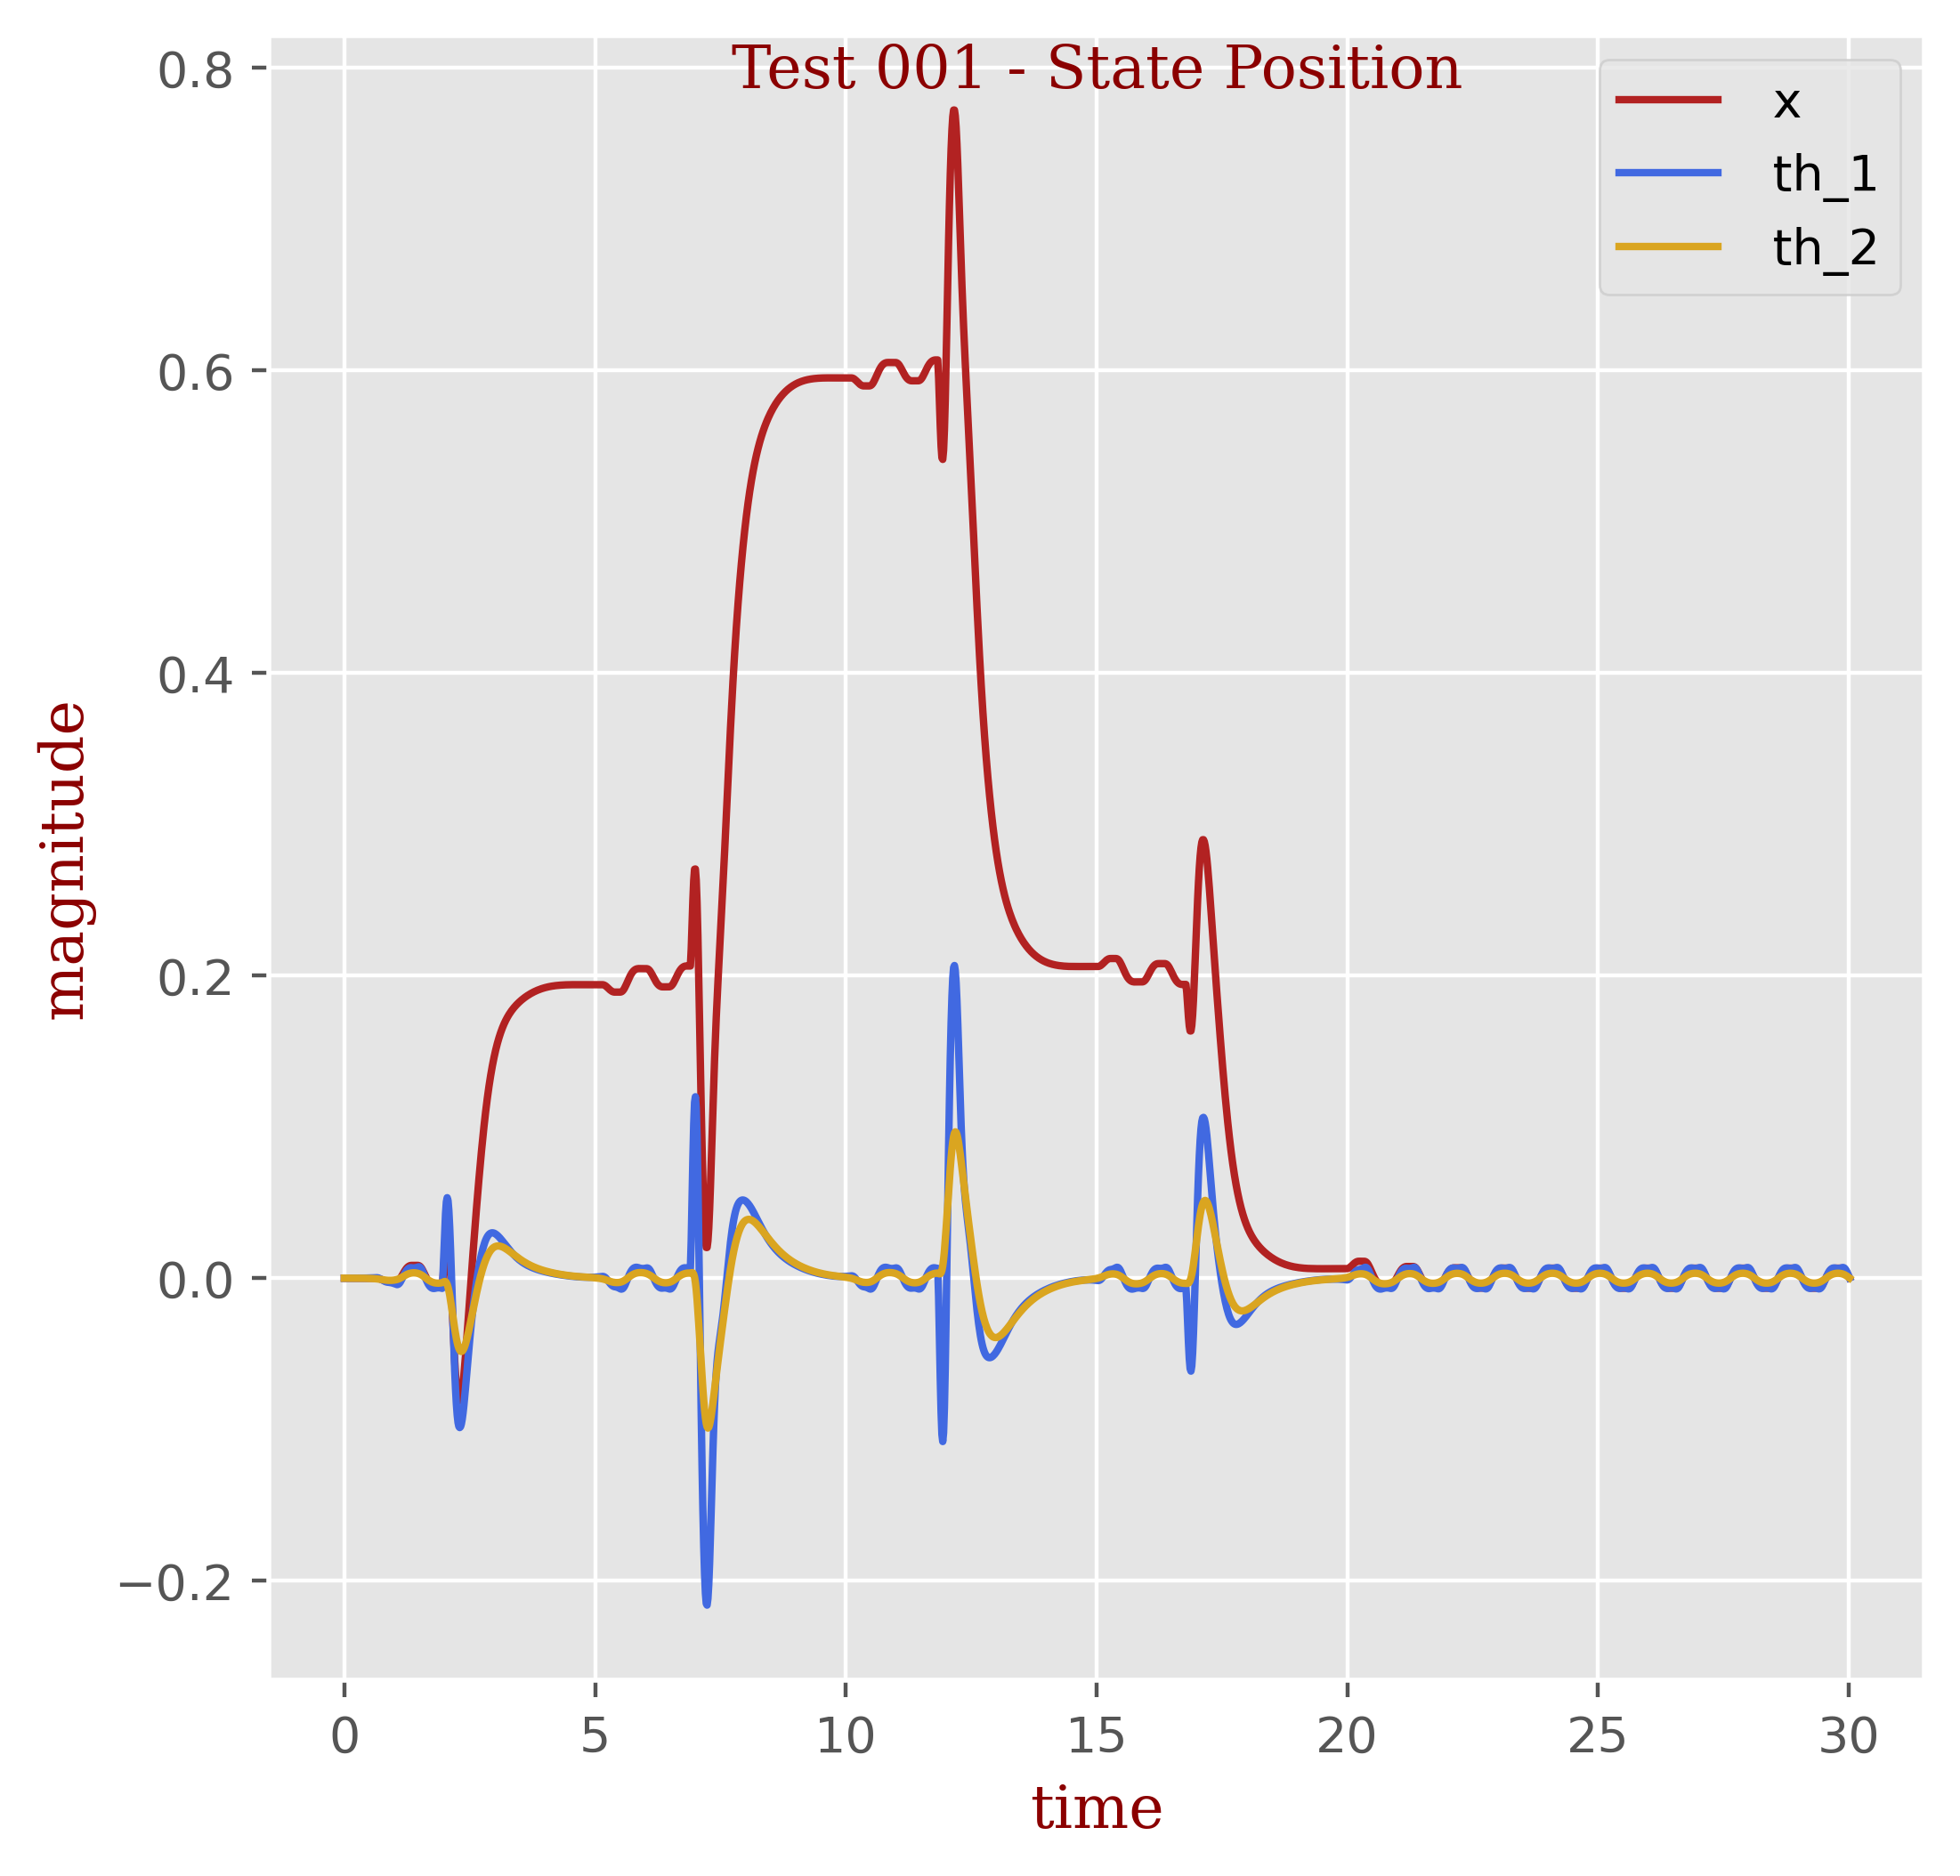
\includegraphics[width=27mm]{Test 001_State_Position.png}}
    \subfigure[\(\dot{q}(t)\)]{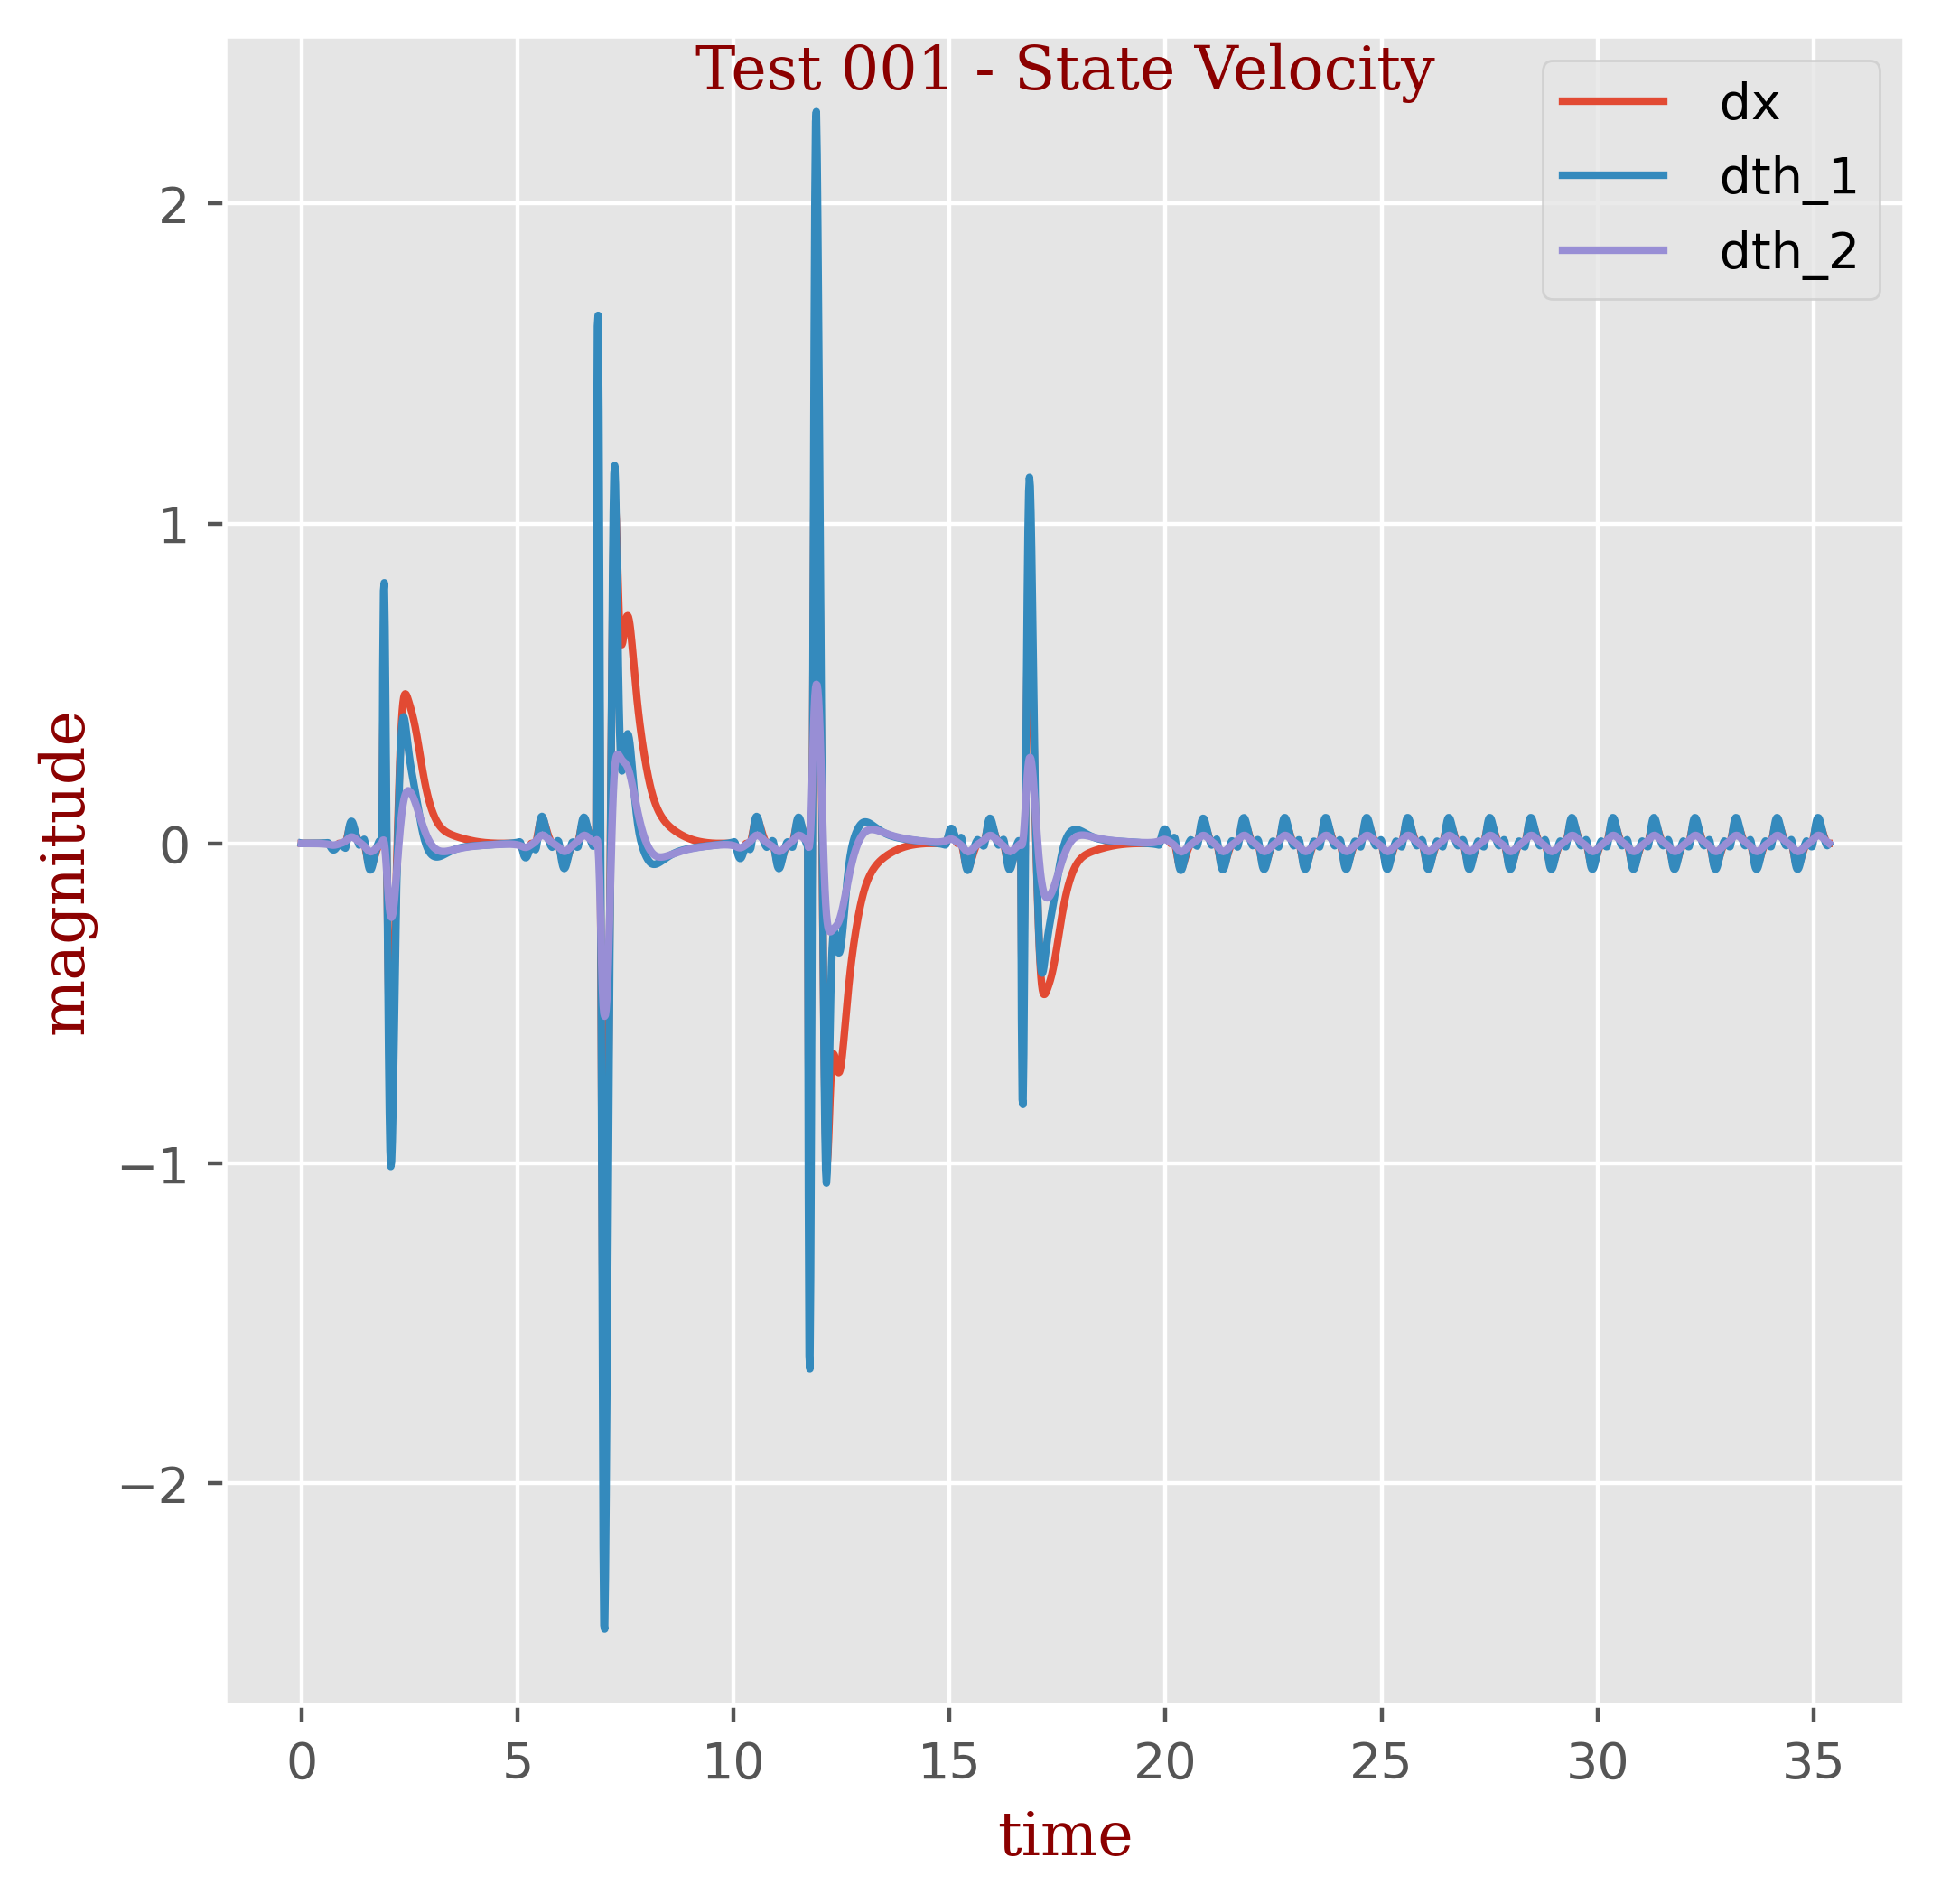
\includegraphics[width=27mm]{Test 001_State_Velocity.png}}
    \subfigure[\(J(t)\)]{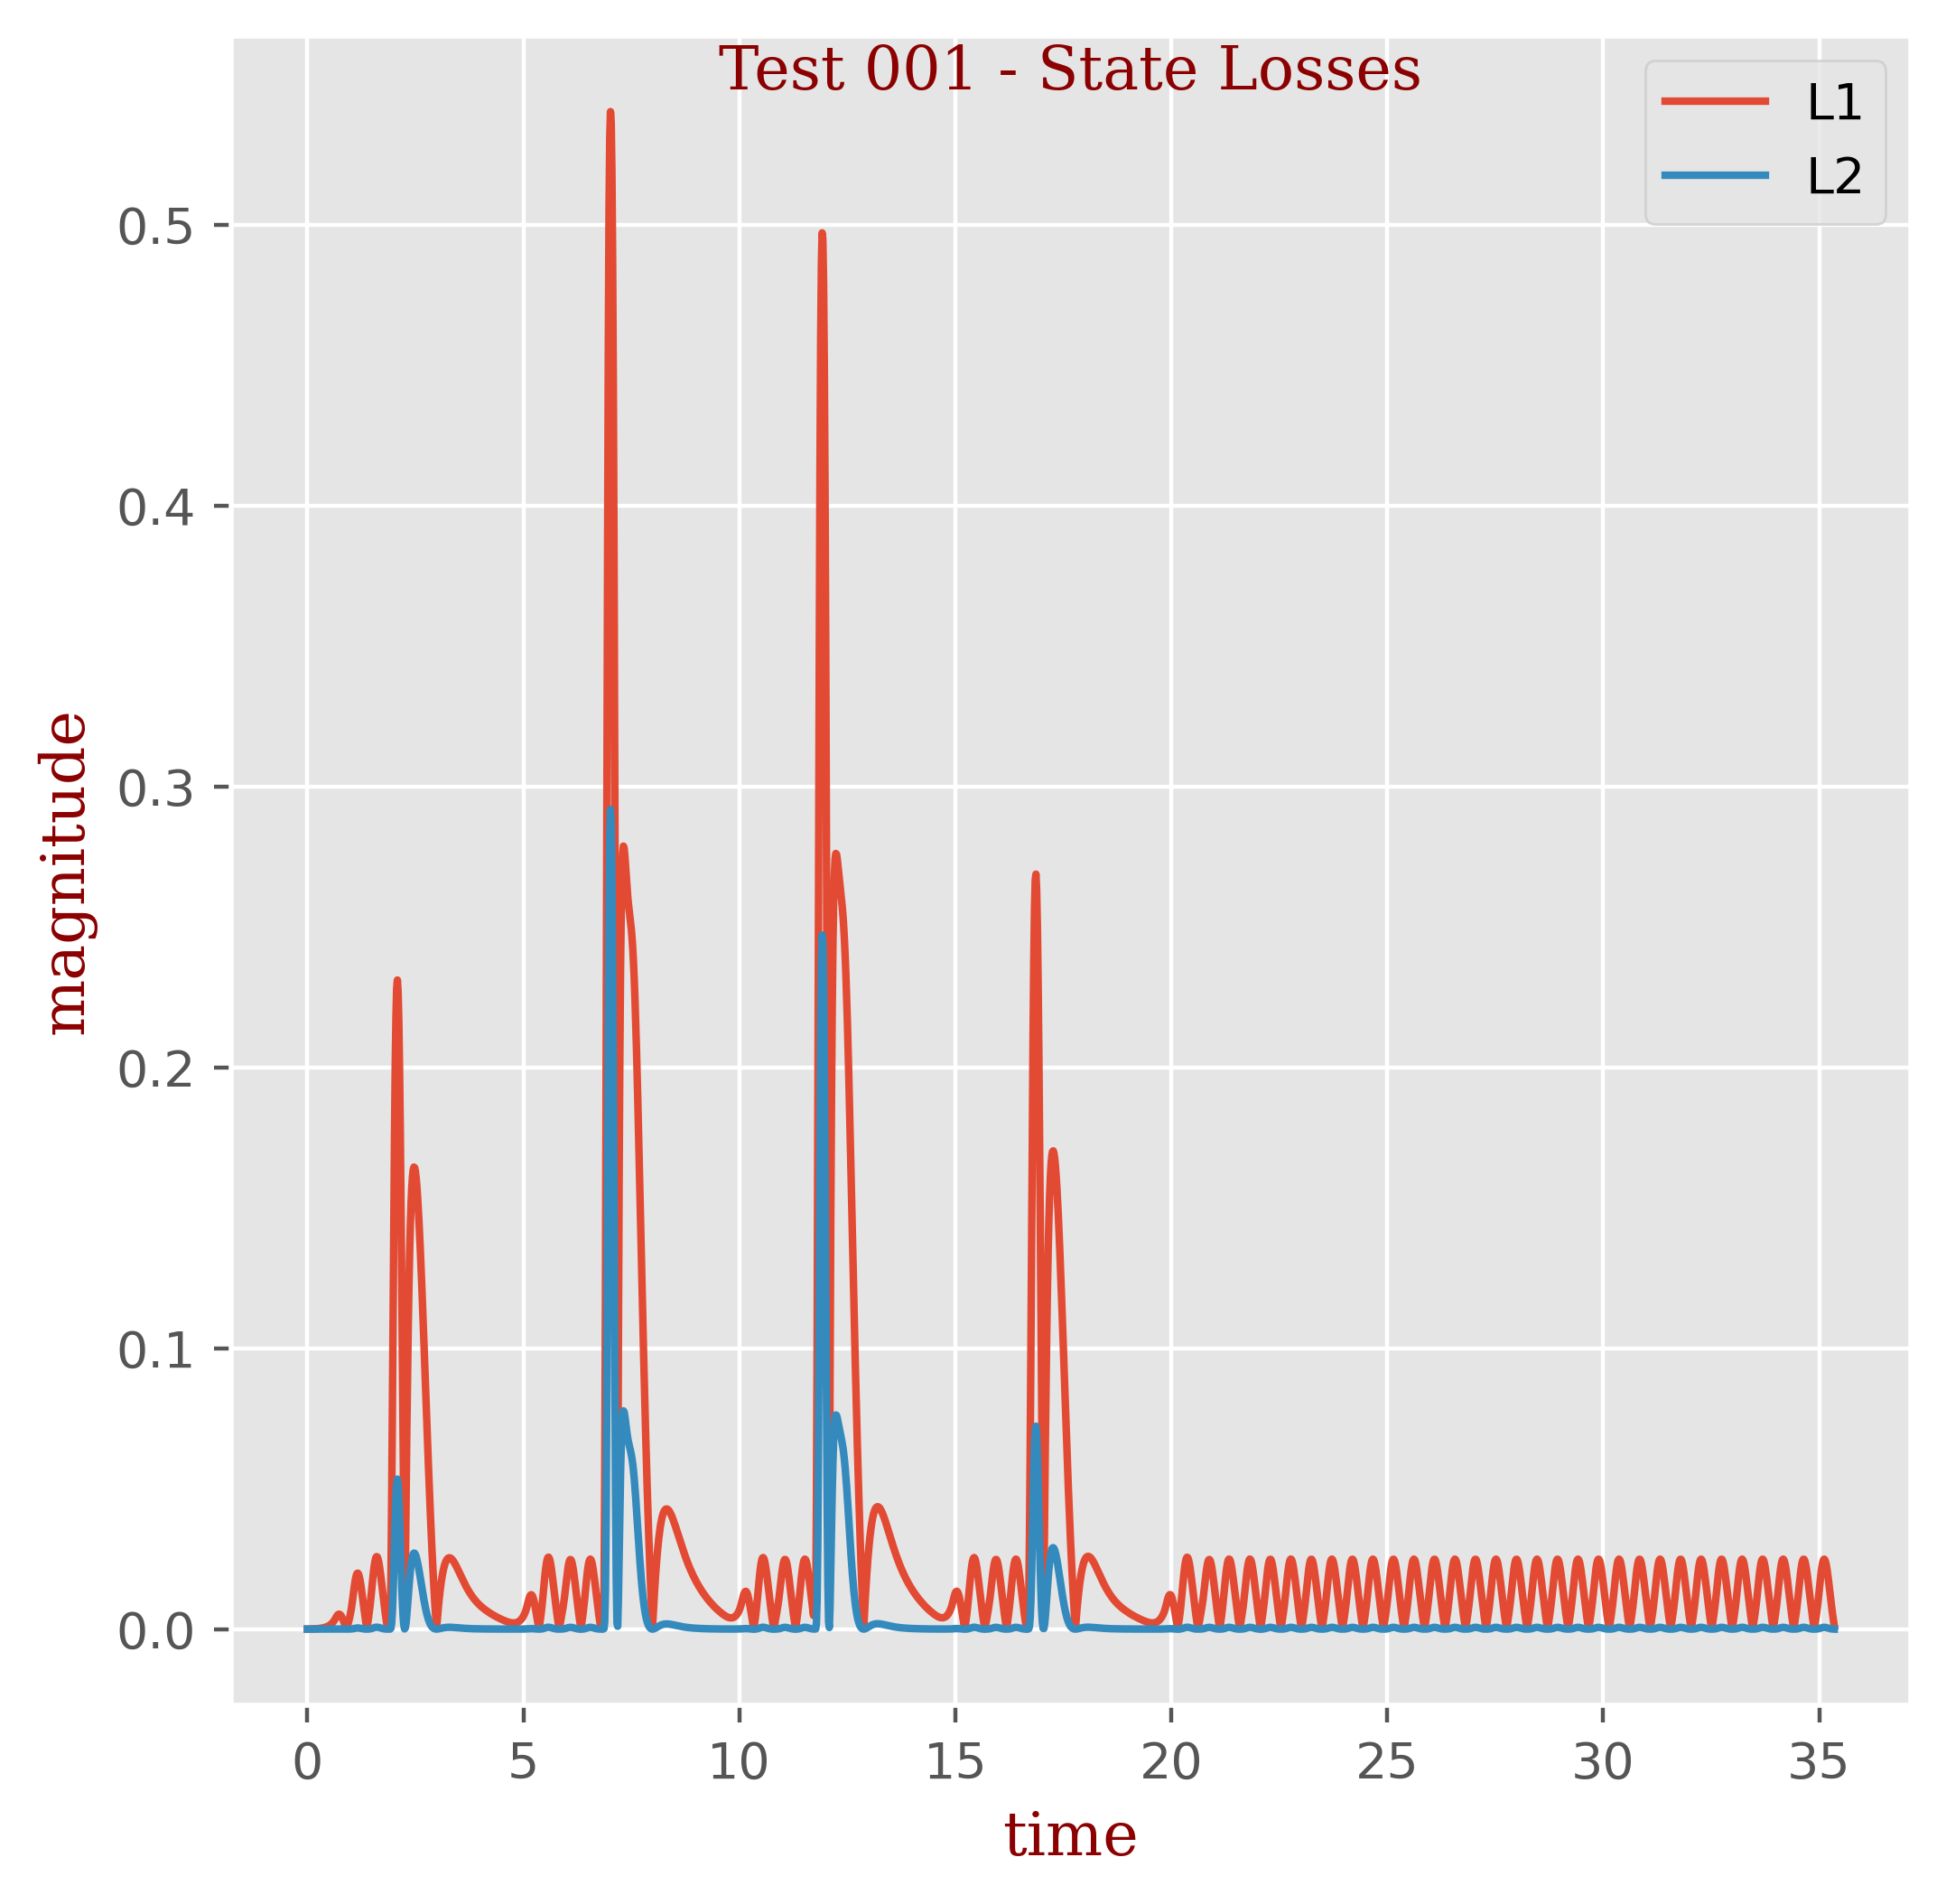
\includegraphics[width=27mm]{Test 001_State_Losses.png}}
    \caption{Test 001}
    \label{fig:t001}
    \end{figure}

\begin{figure}
\centering
\subfigure[\(q(t)\)]{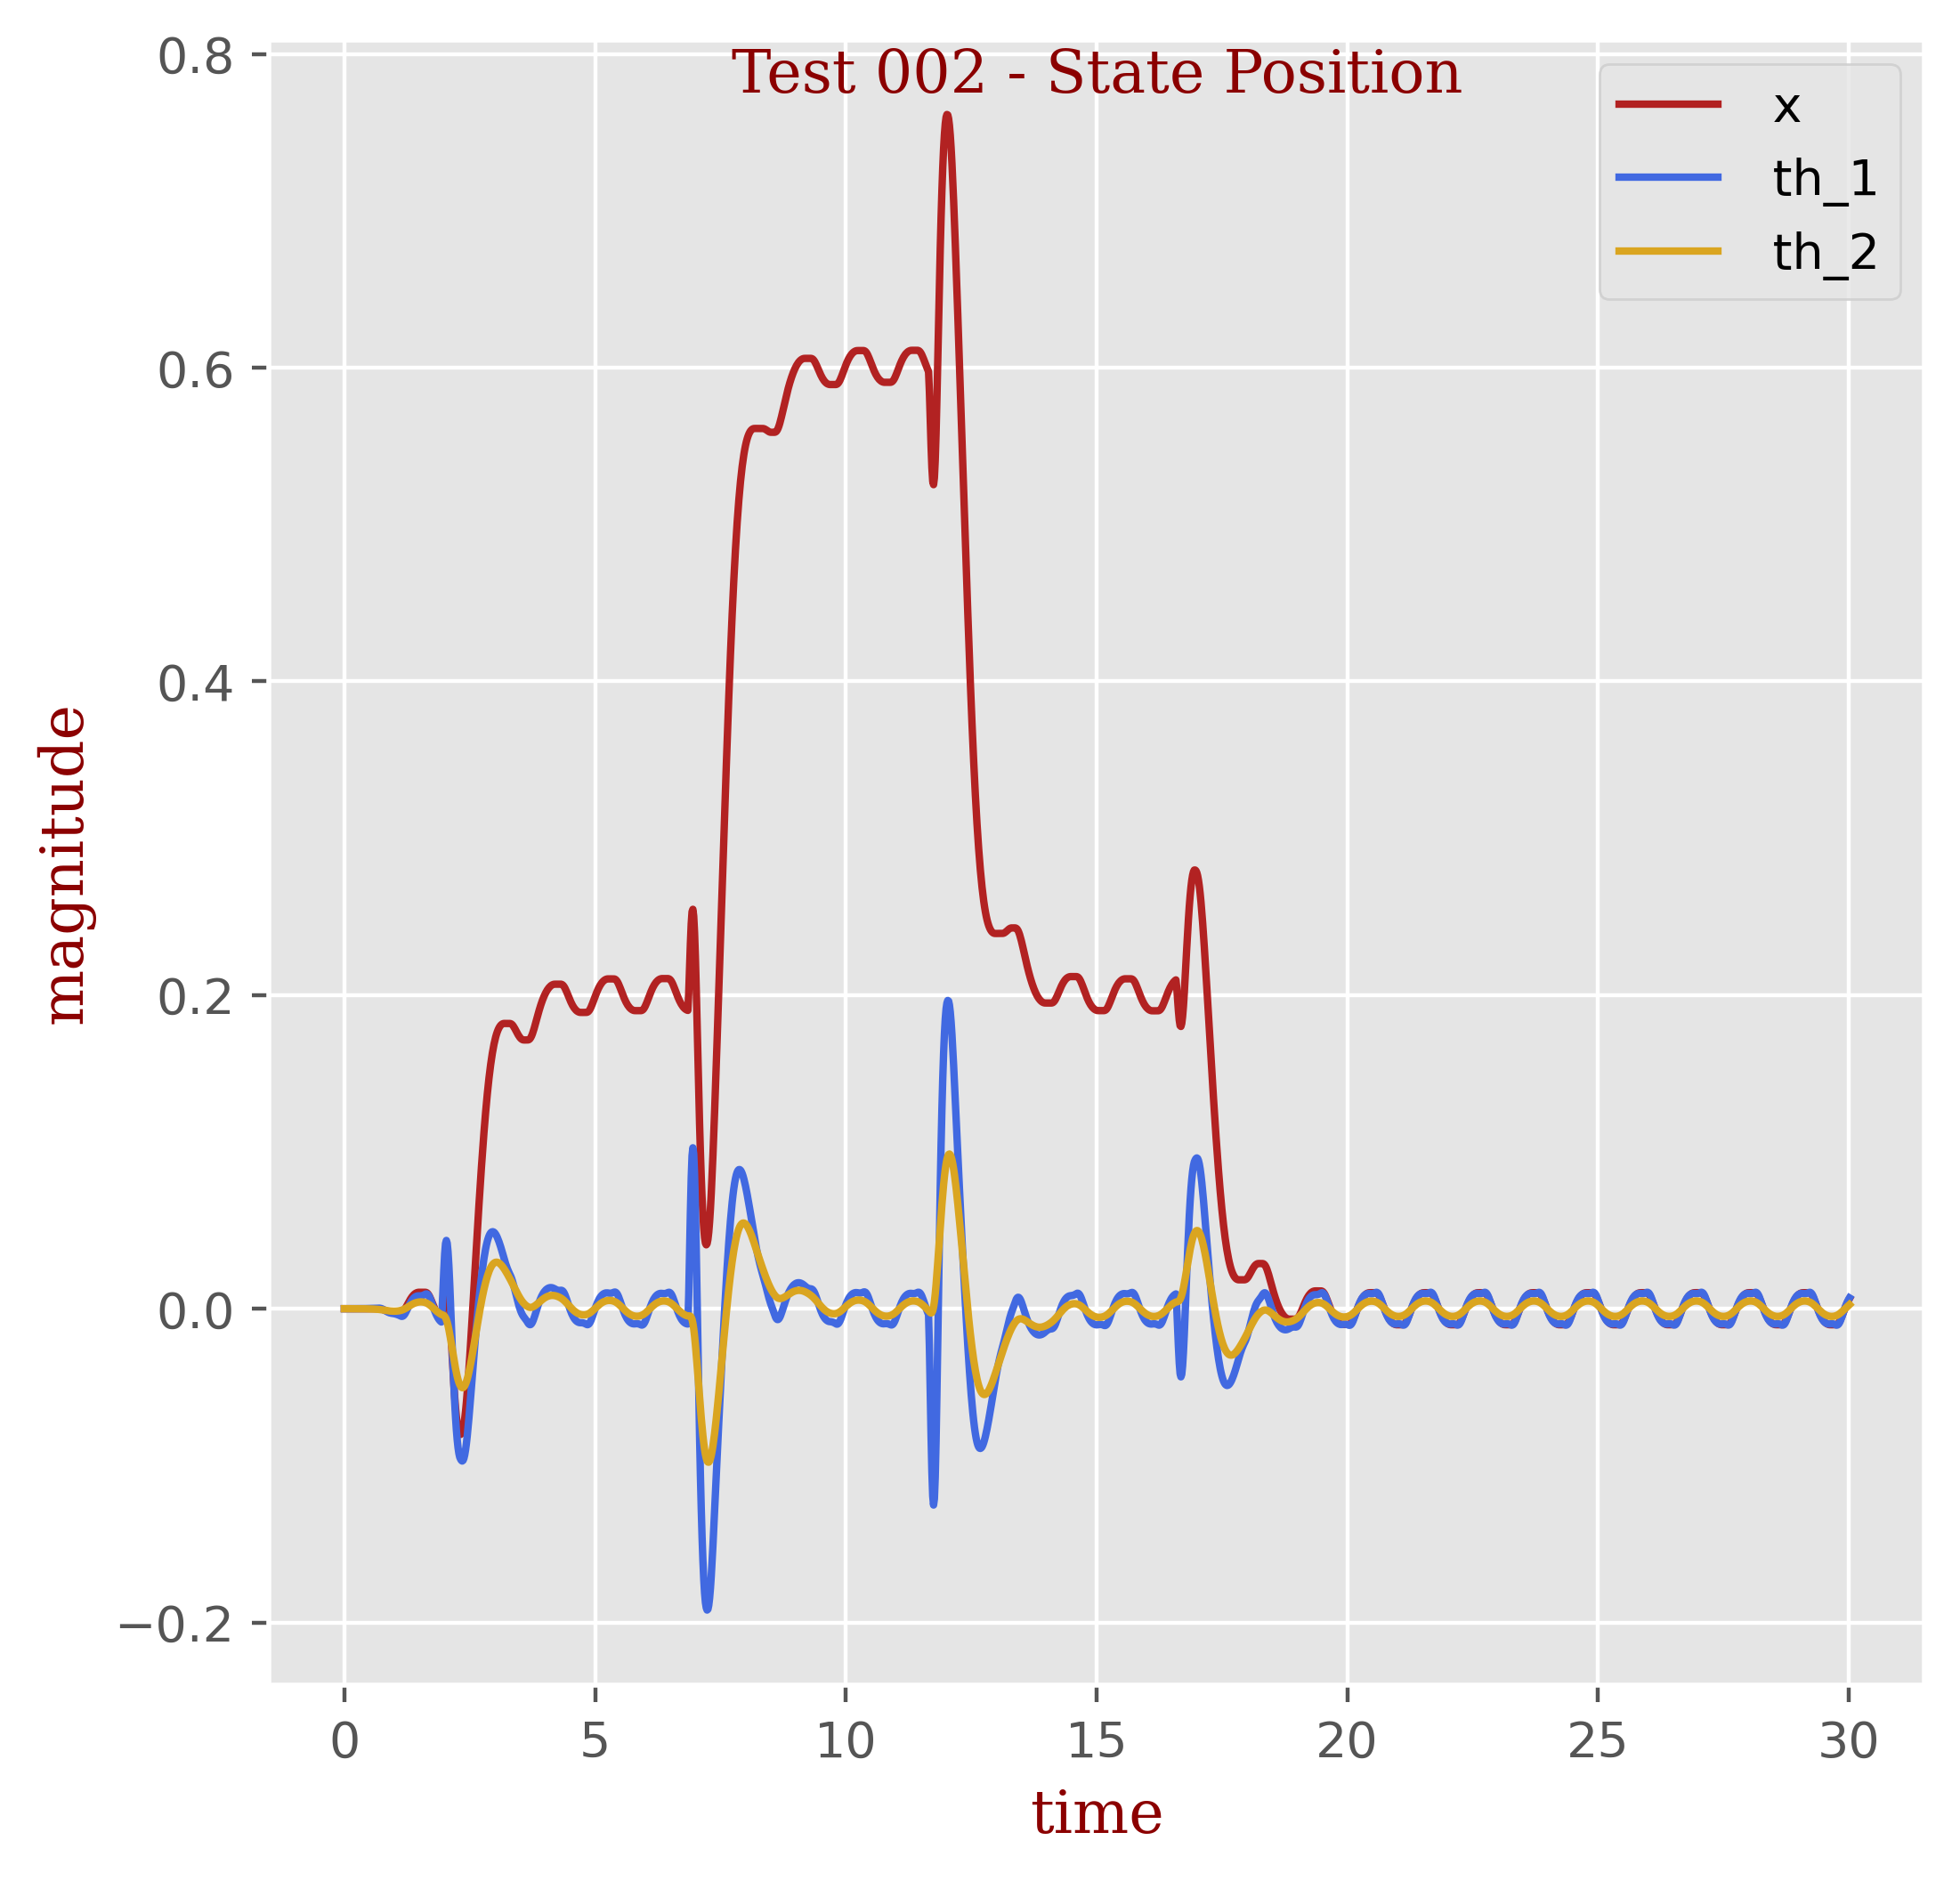
\includegraphics[width=27mm]{Test 002_State_Position.png}}
\subfigure[\(\dot{q}(t)\)]{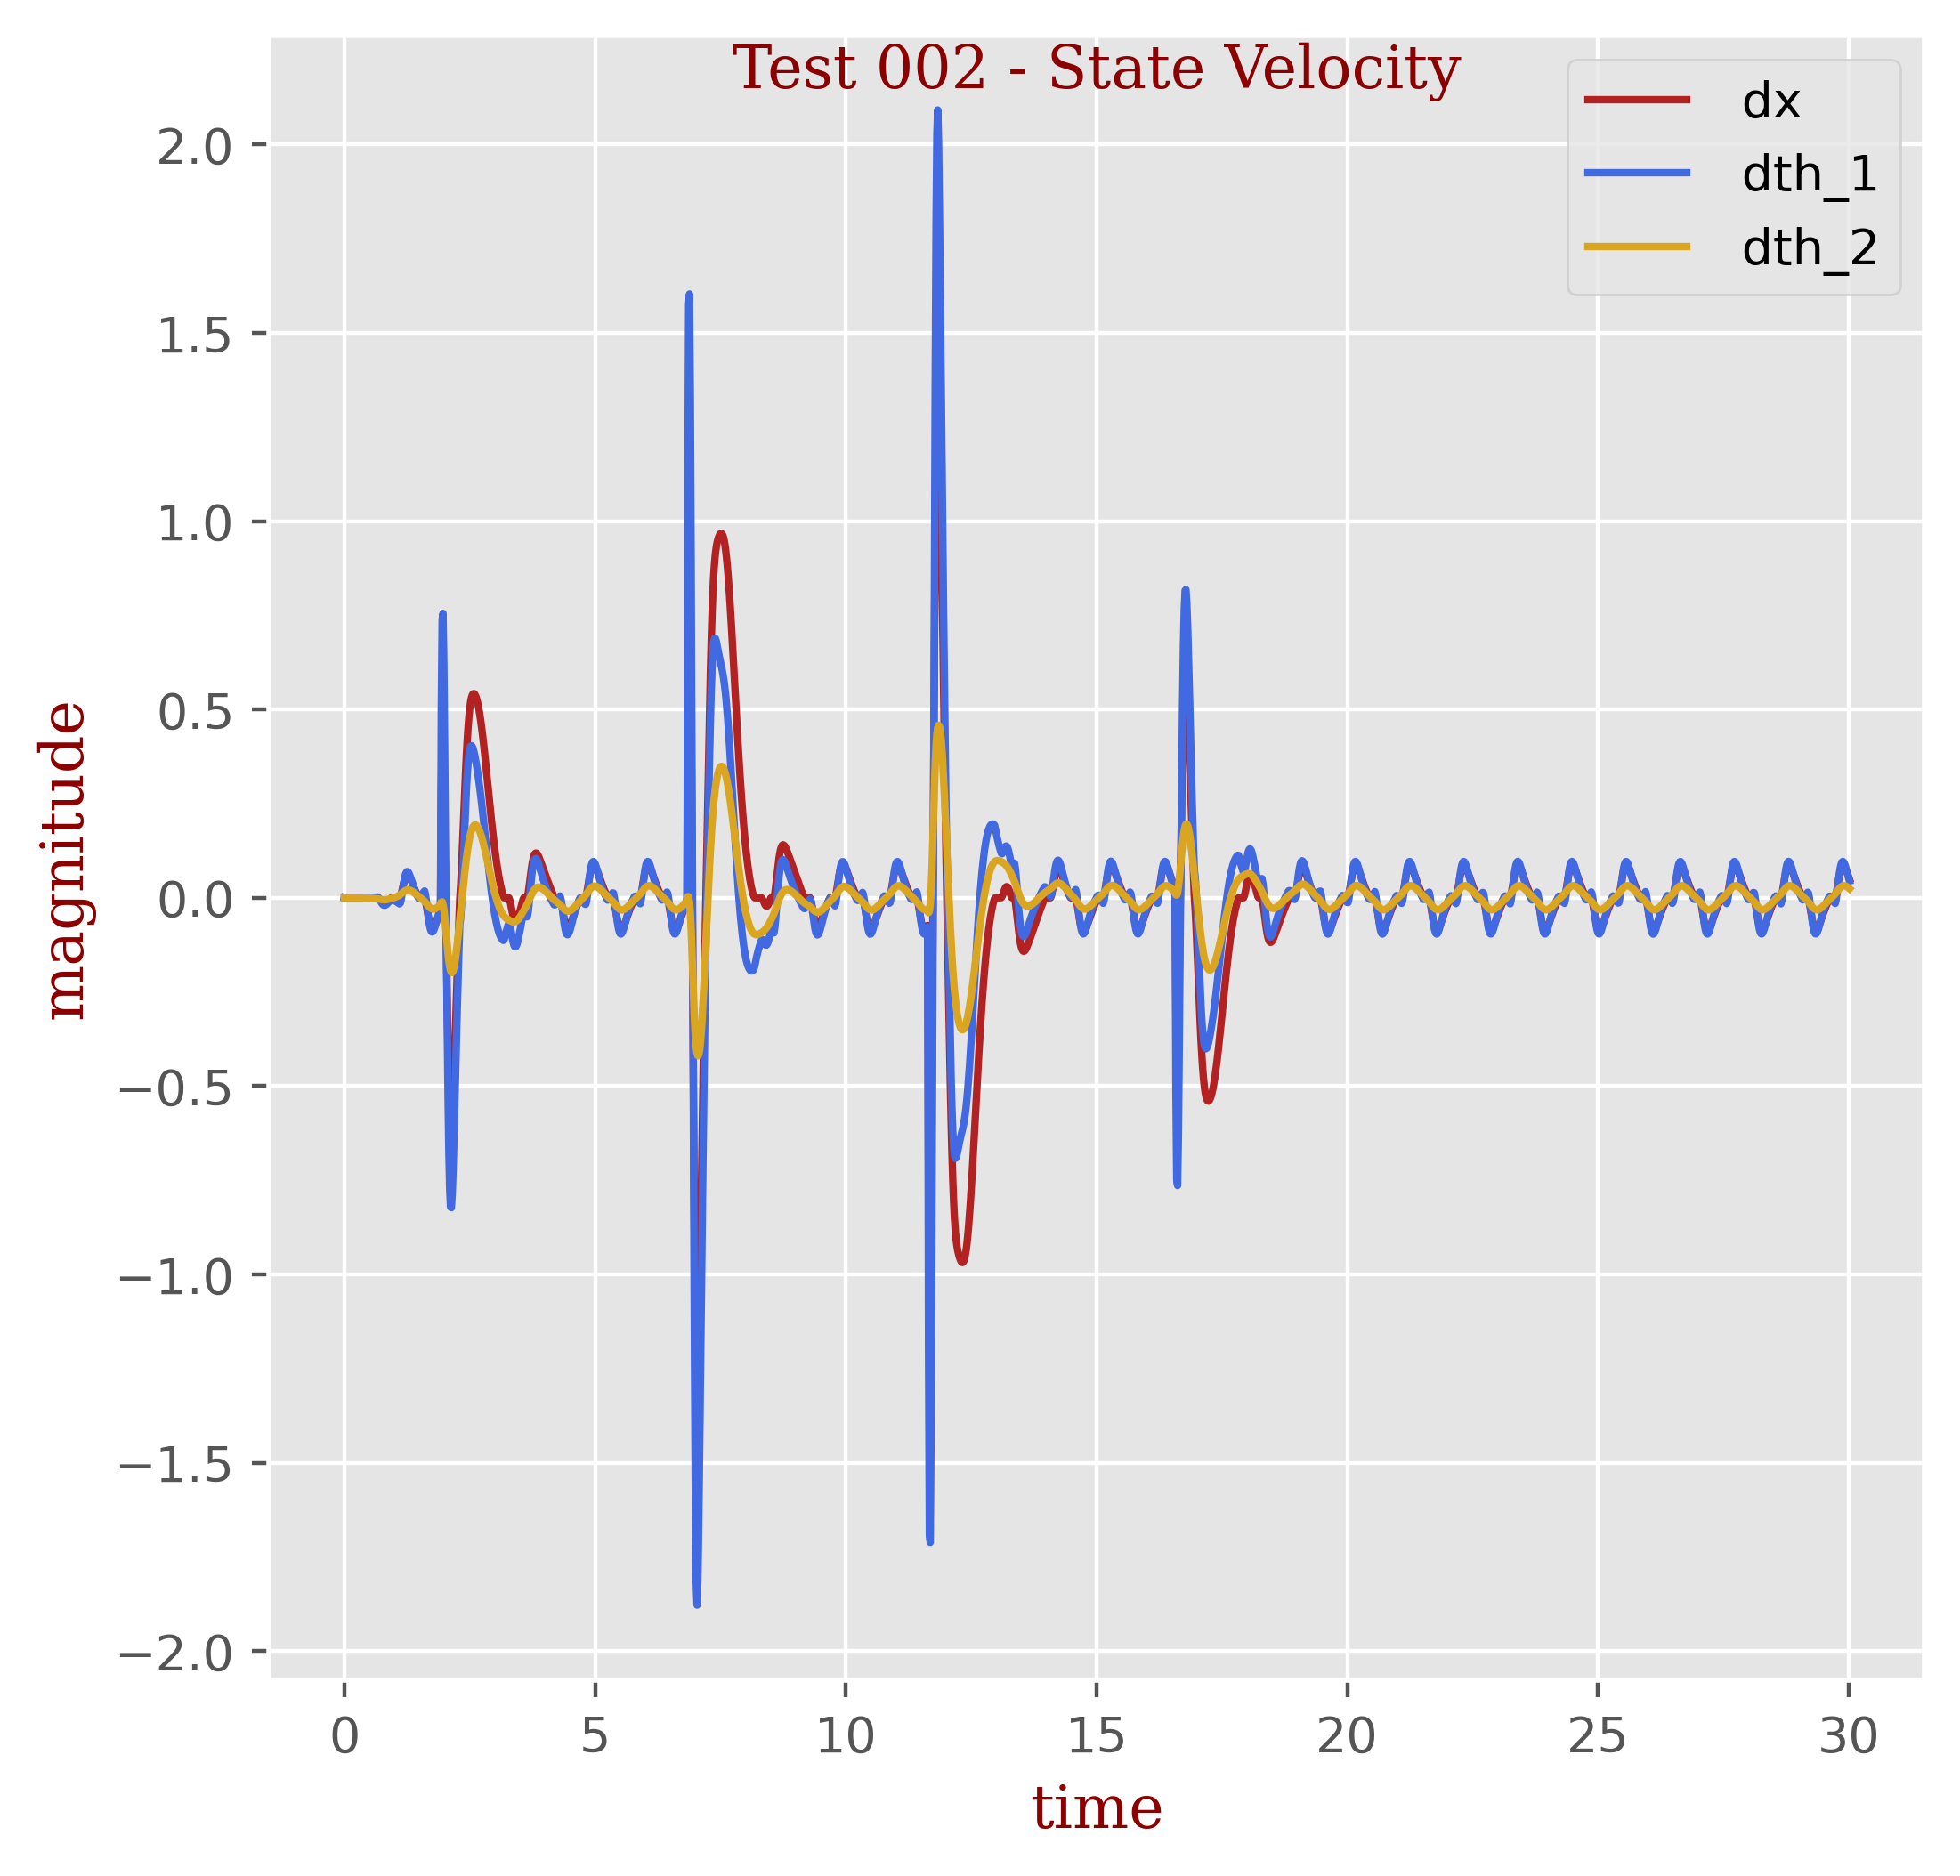
\includegraphics[width=27mm]{Test 002_State_Velocity.png}}
\subfigure[\(J(t)\)]{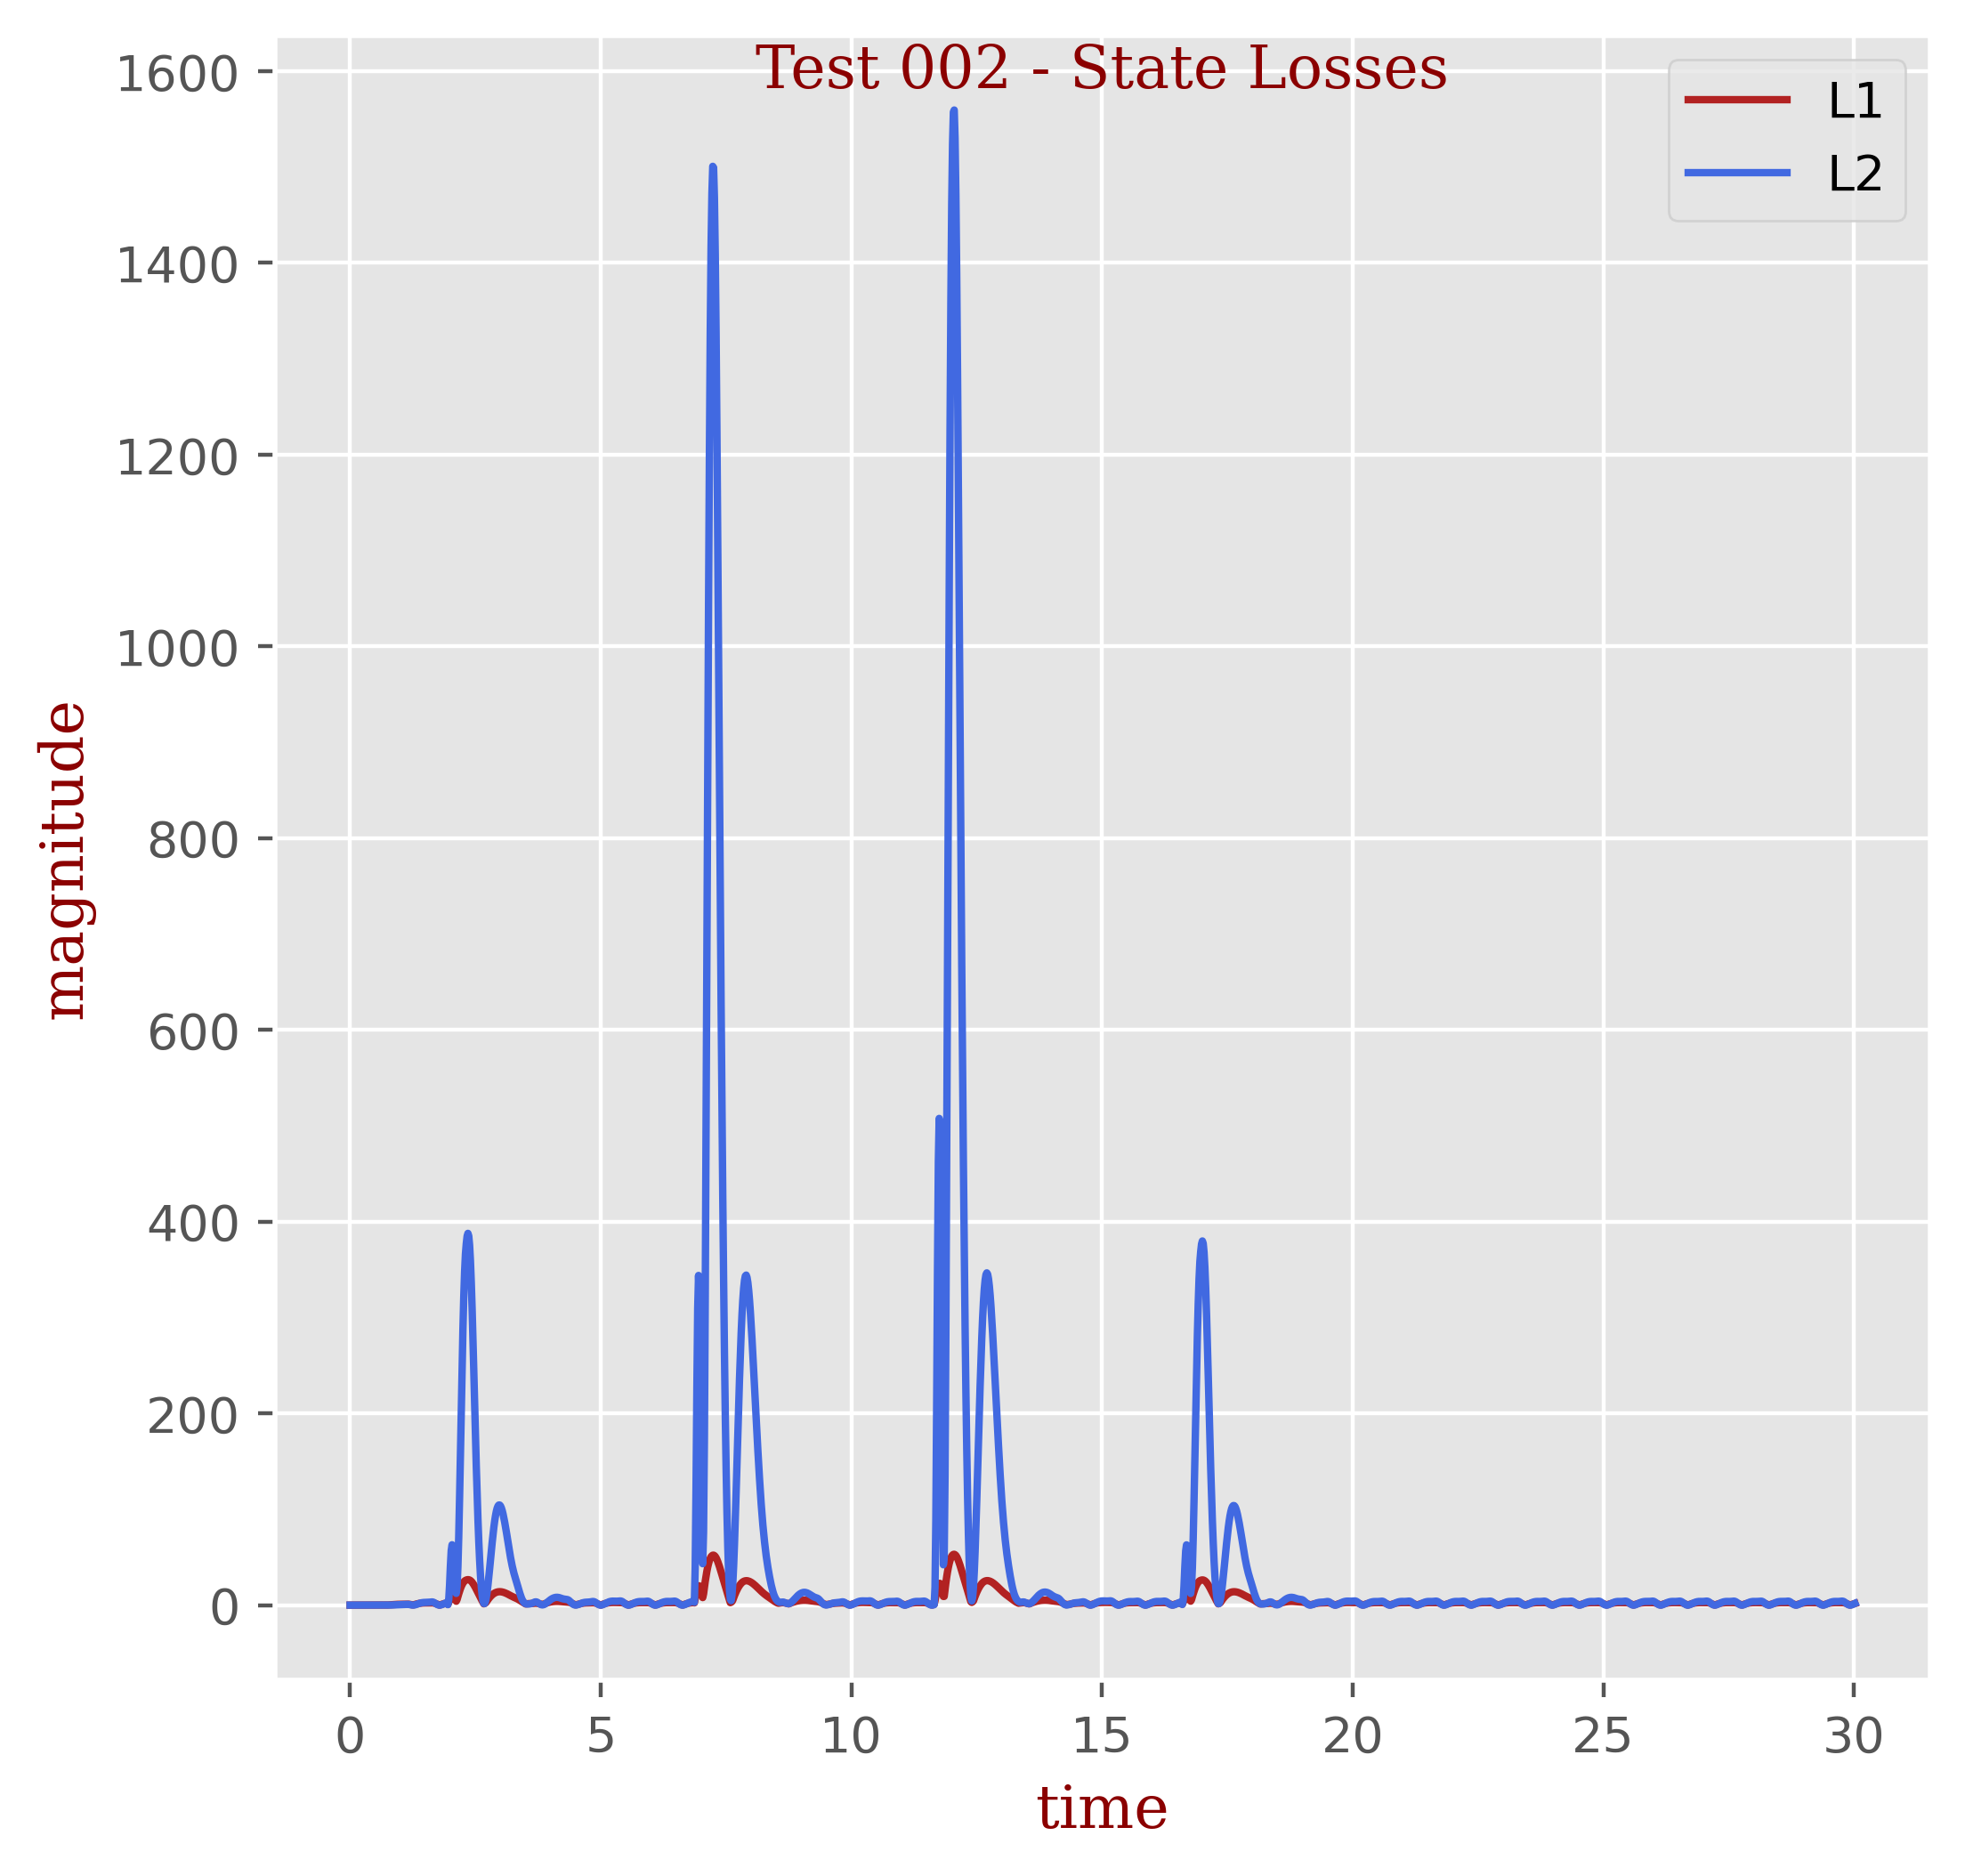
\includegraphics[width=27mm]{Test 002_State_Losses.png}}
\caption{Test 002}
\label{fig:t002}
\end{figure}

\begin{figure}
\centering
      \subfigure[\(q(t)\)]{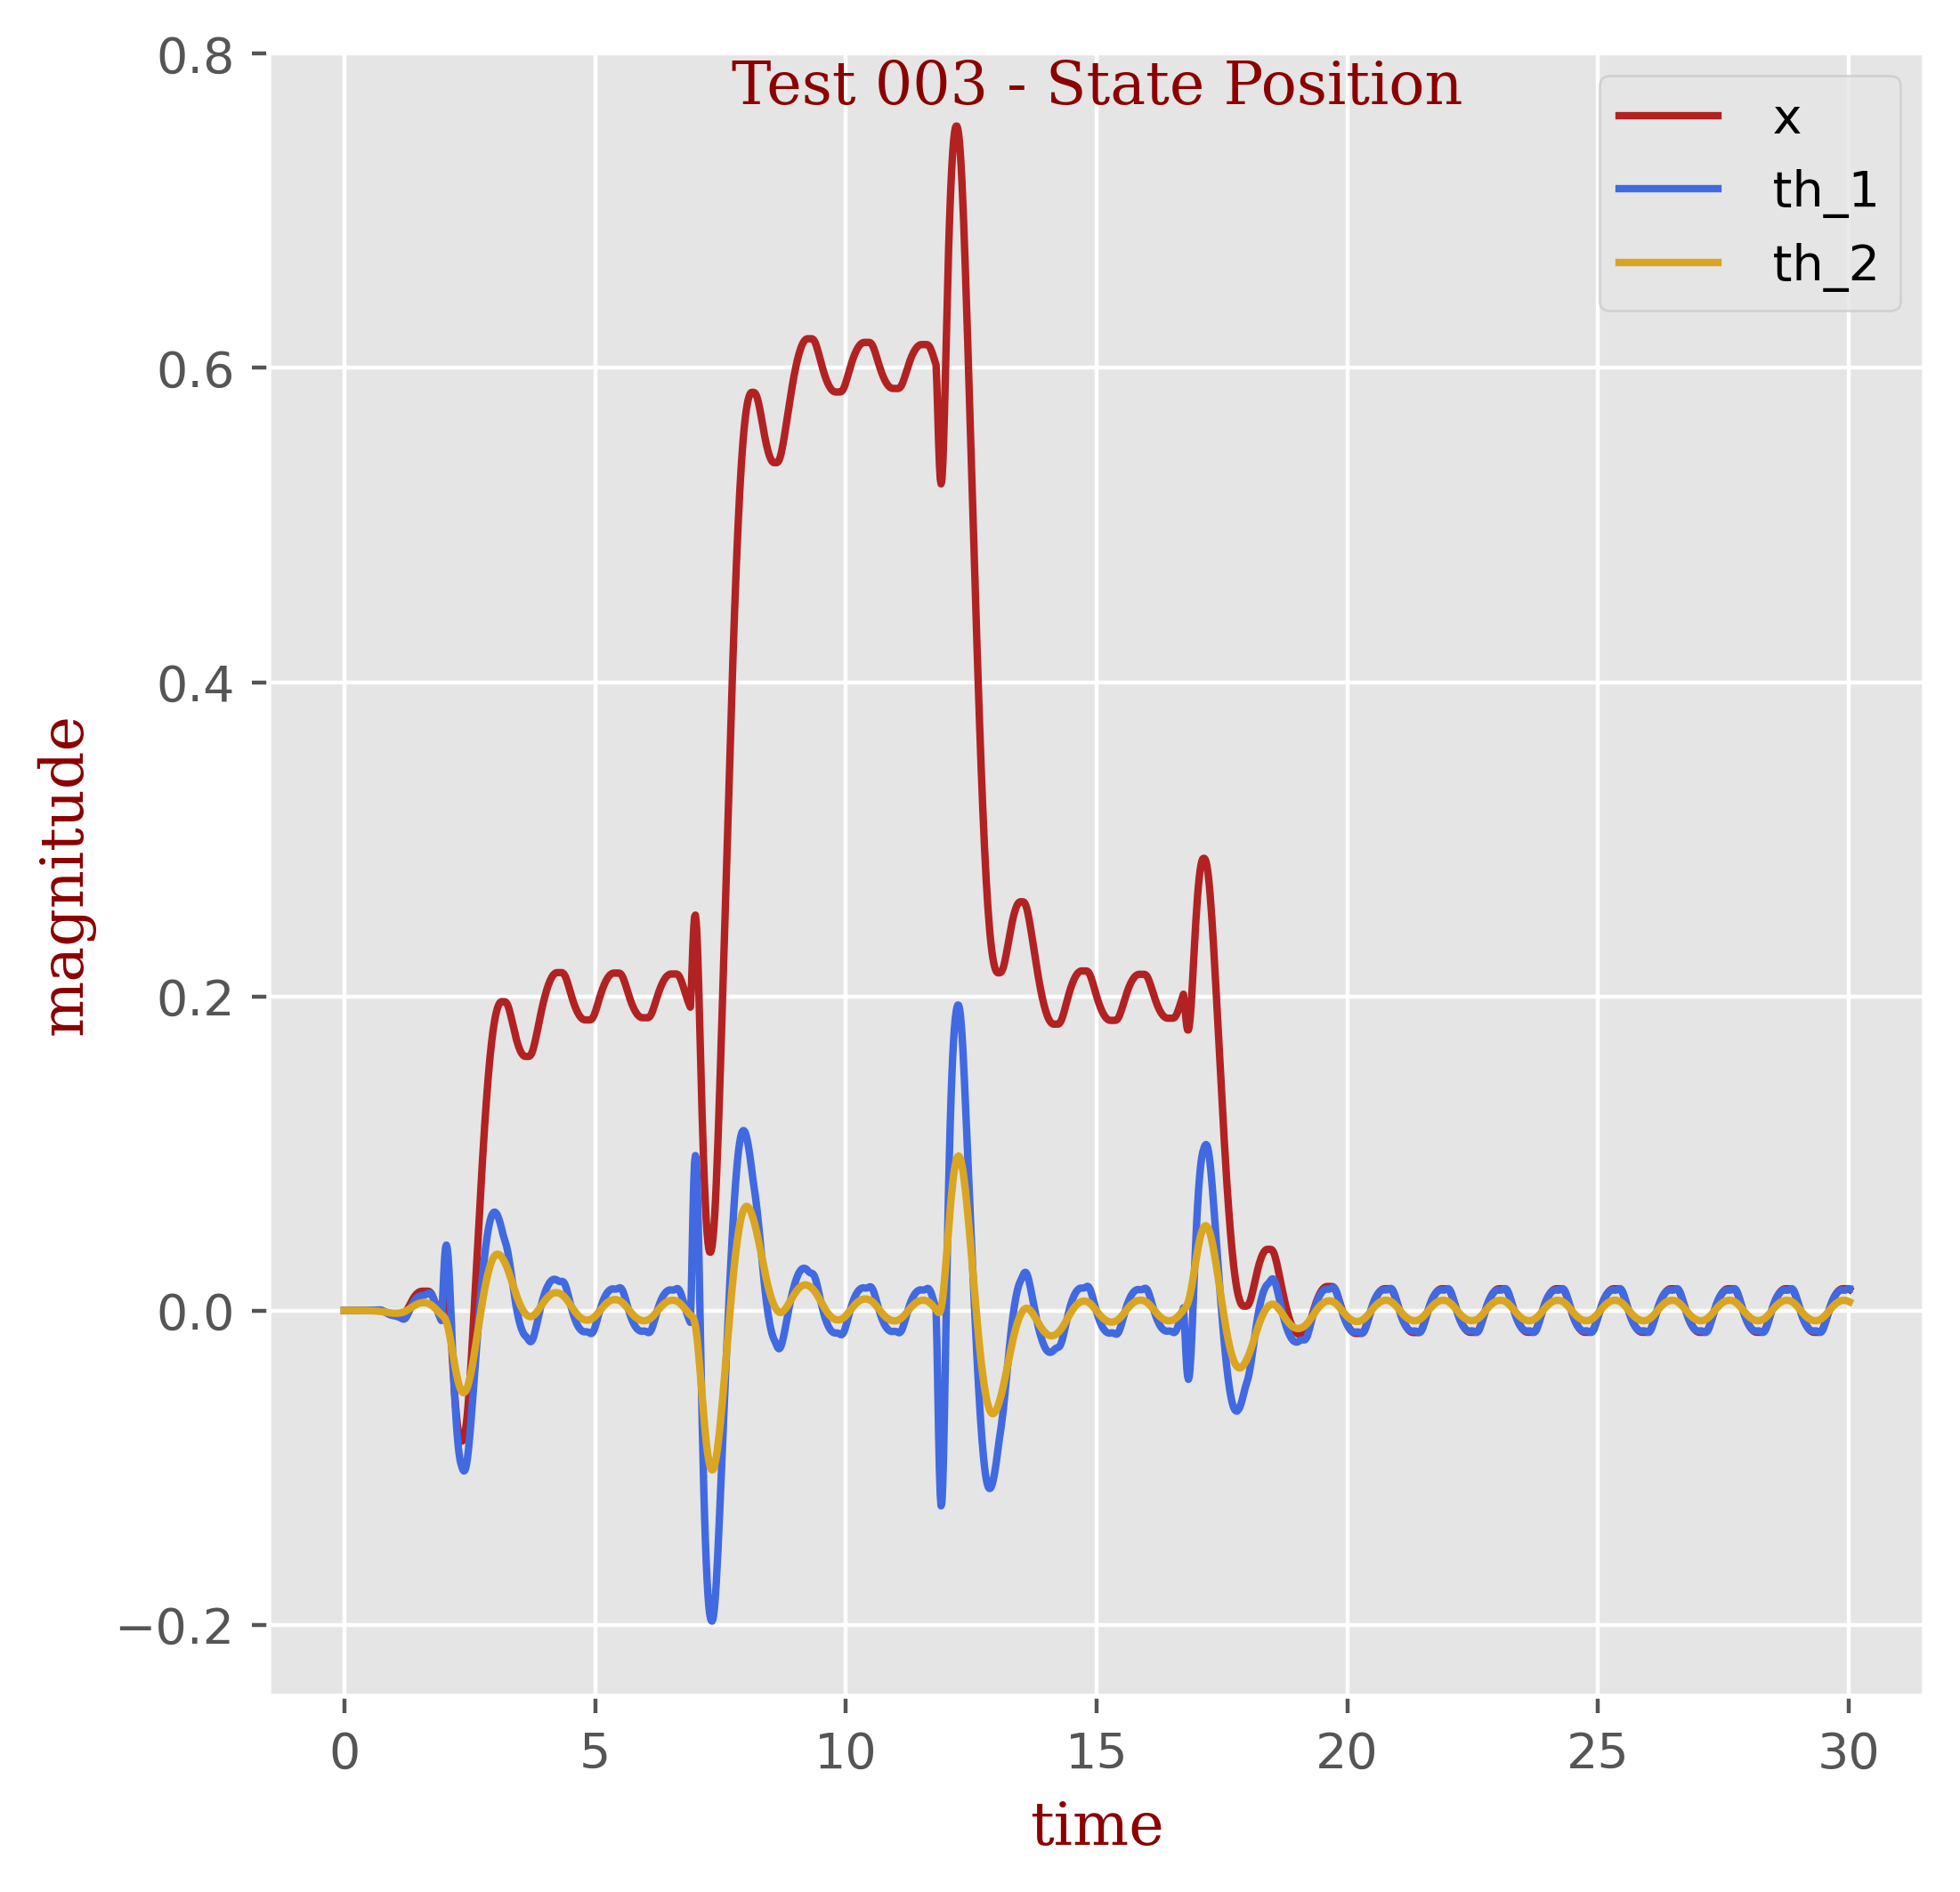
\includegraphics[width=27mm]{Test 003_State_Position.png}}
\subfigure[\(\dot{q}(t)\)]{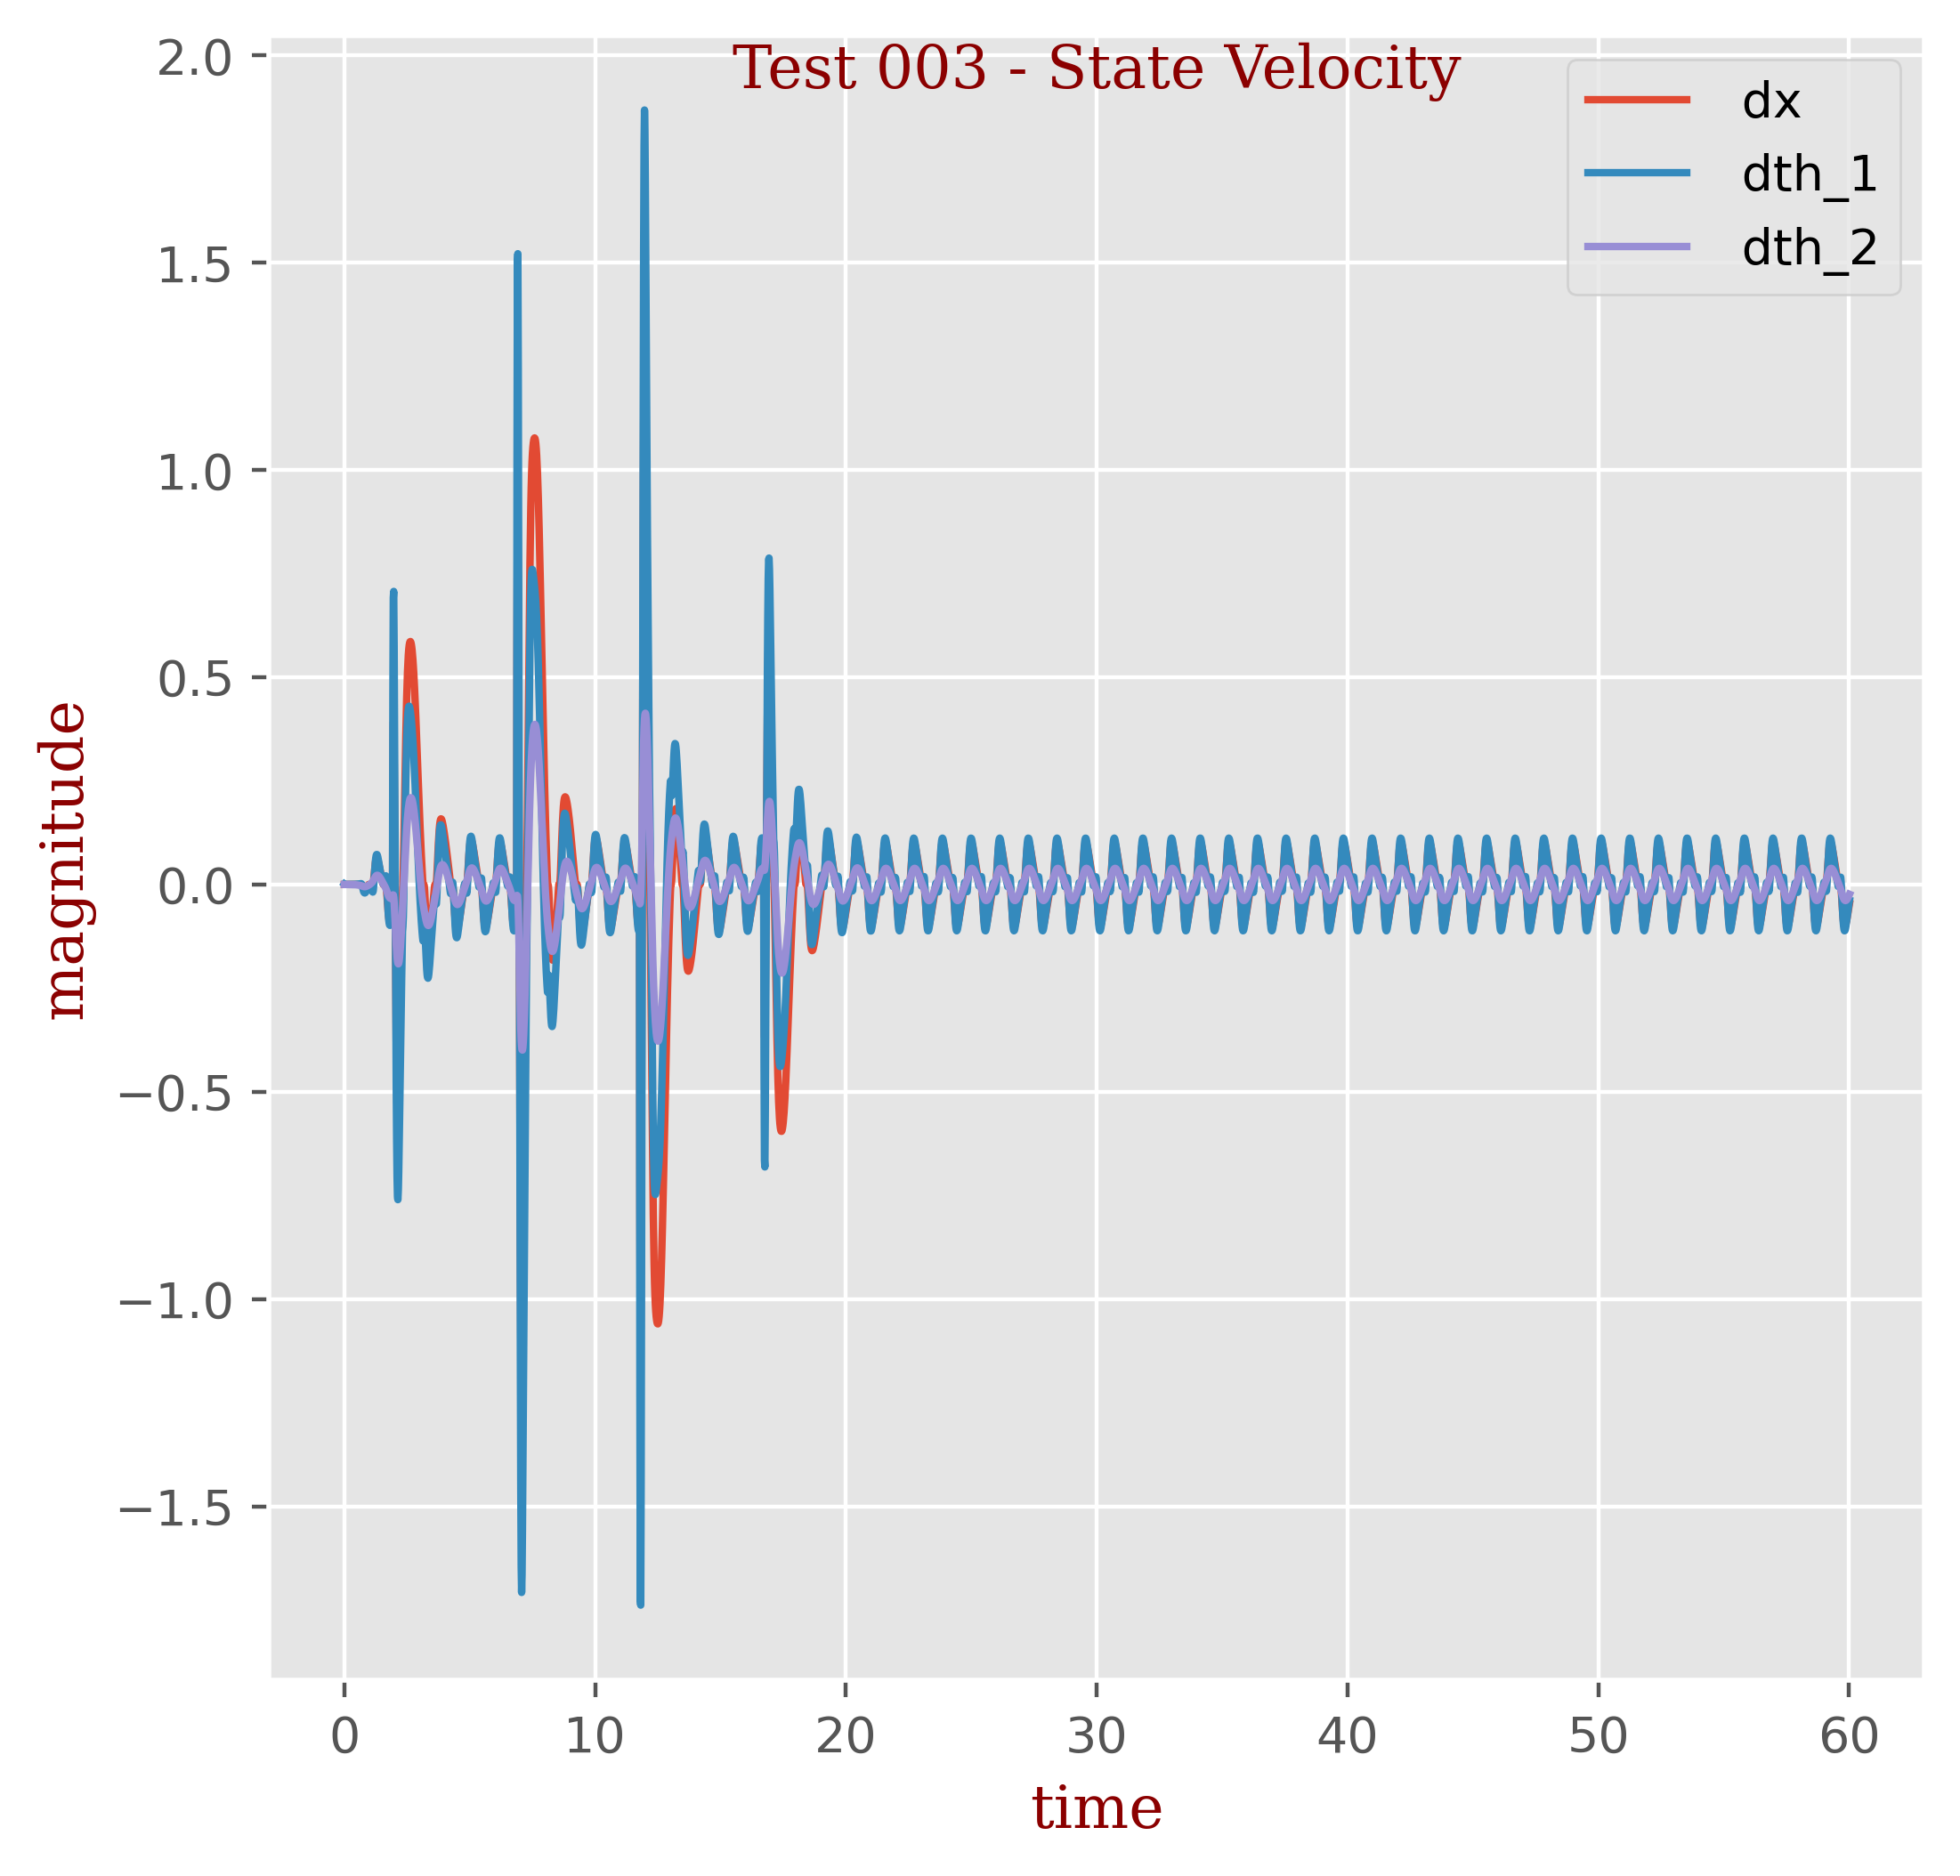
\includegraphics[width=27mm]{Test 003_State_Velocity.png}}
      \subfigure[\(J(t)\)]{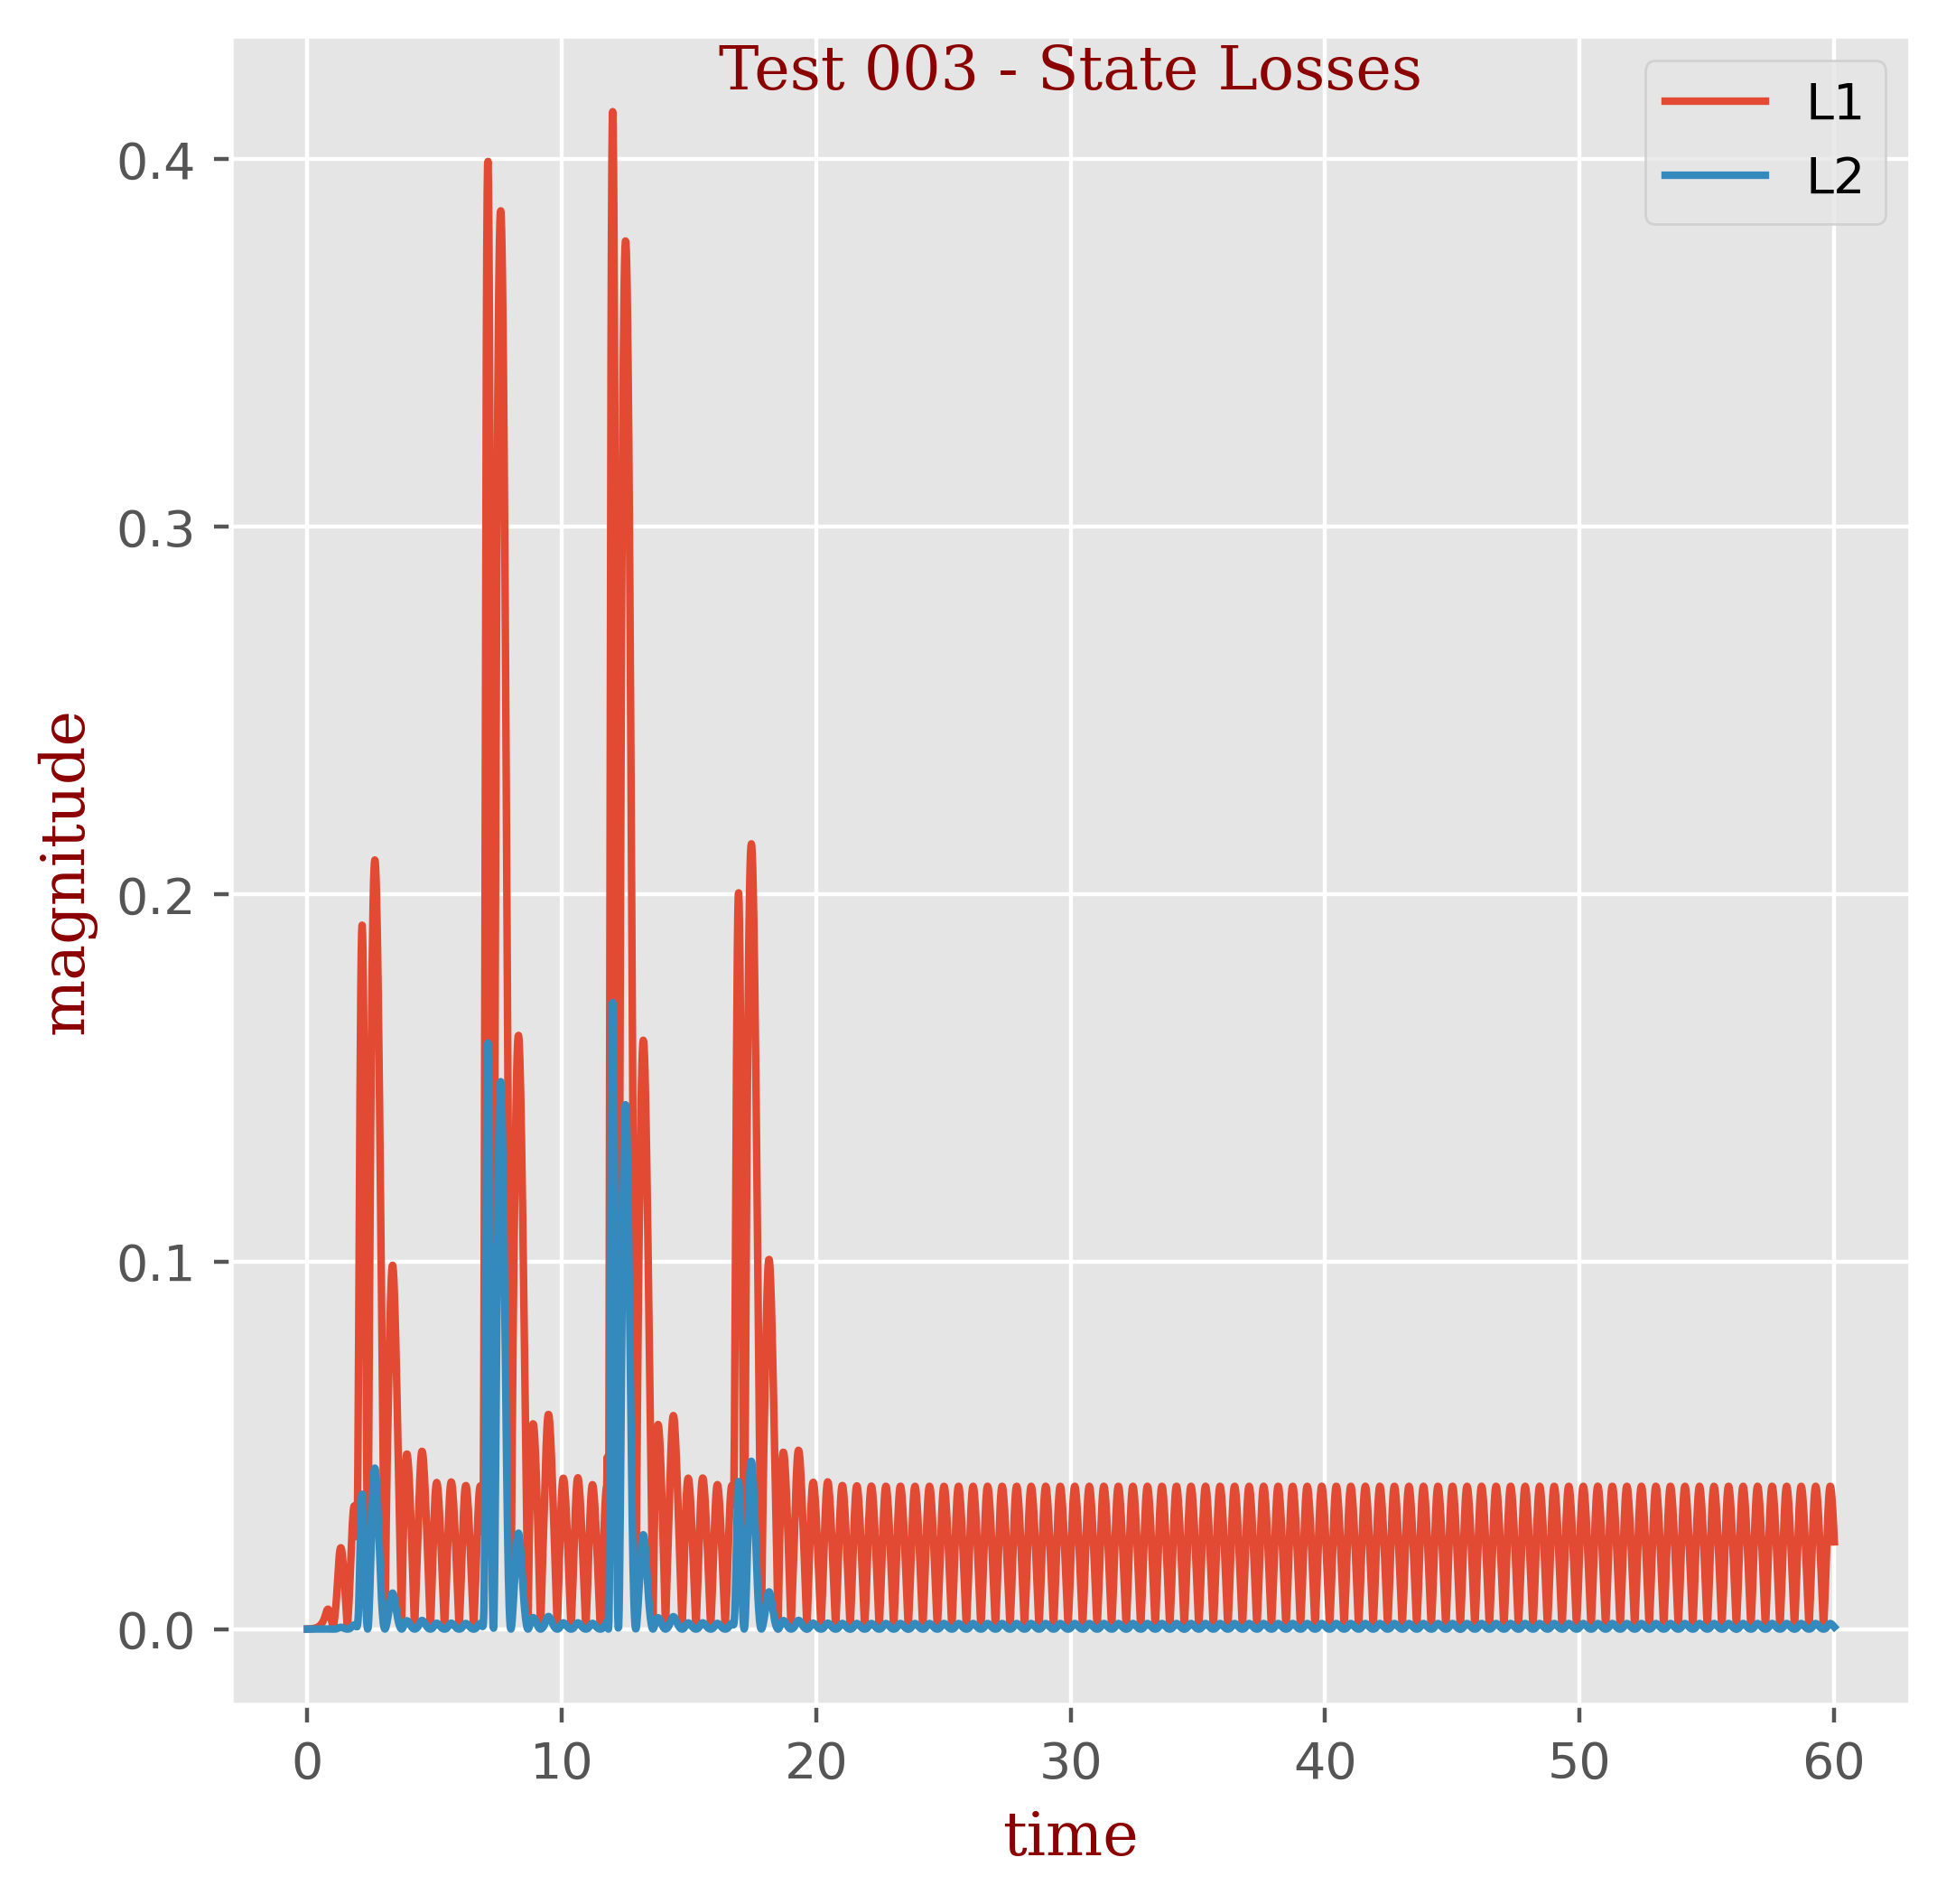
\includegraphics[width=27mm]{Test 003_State_Losses.png}}
\caption{Test 003}
\label{fig:t003}
\end{figure}

\begin{figure}
\centering
      \subfigure[\(q(t)\)]{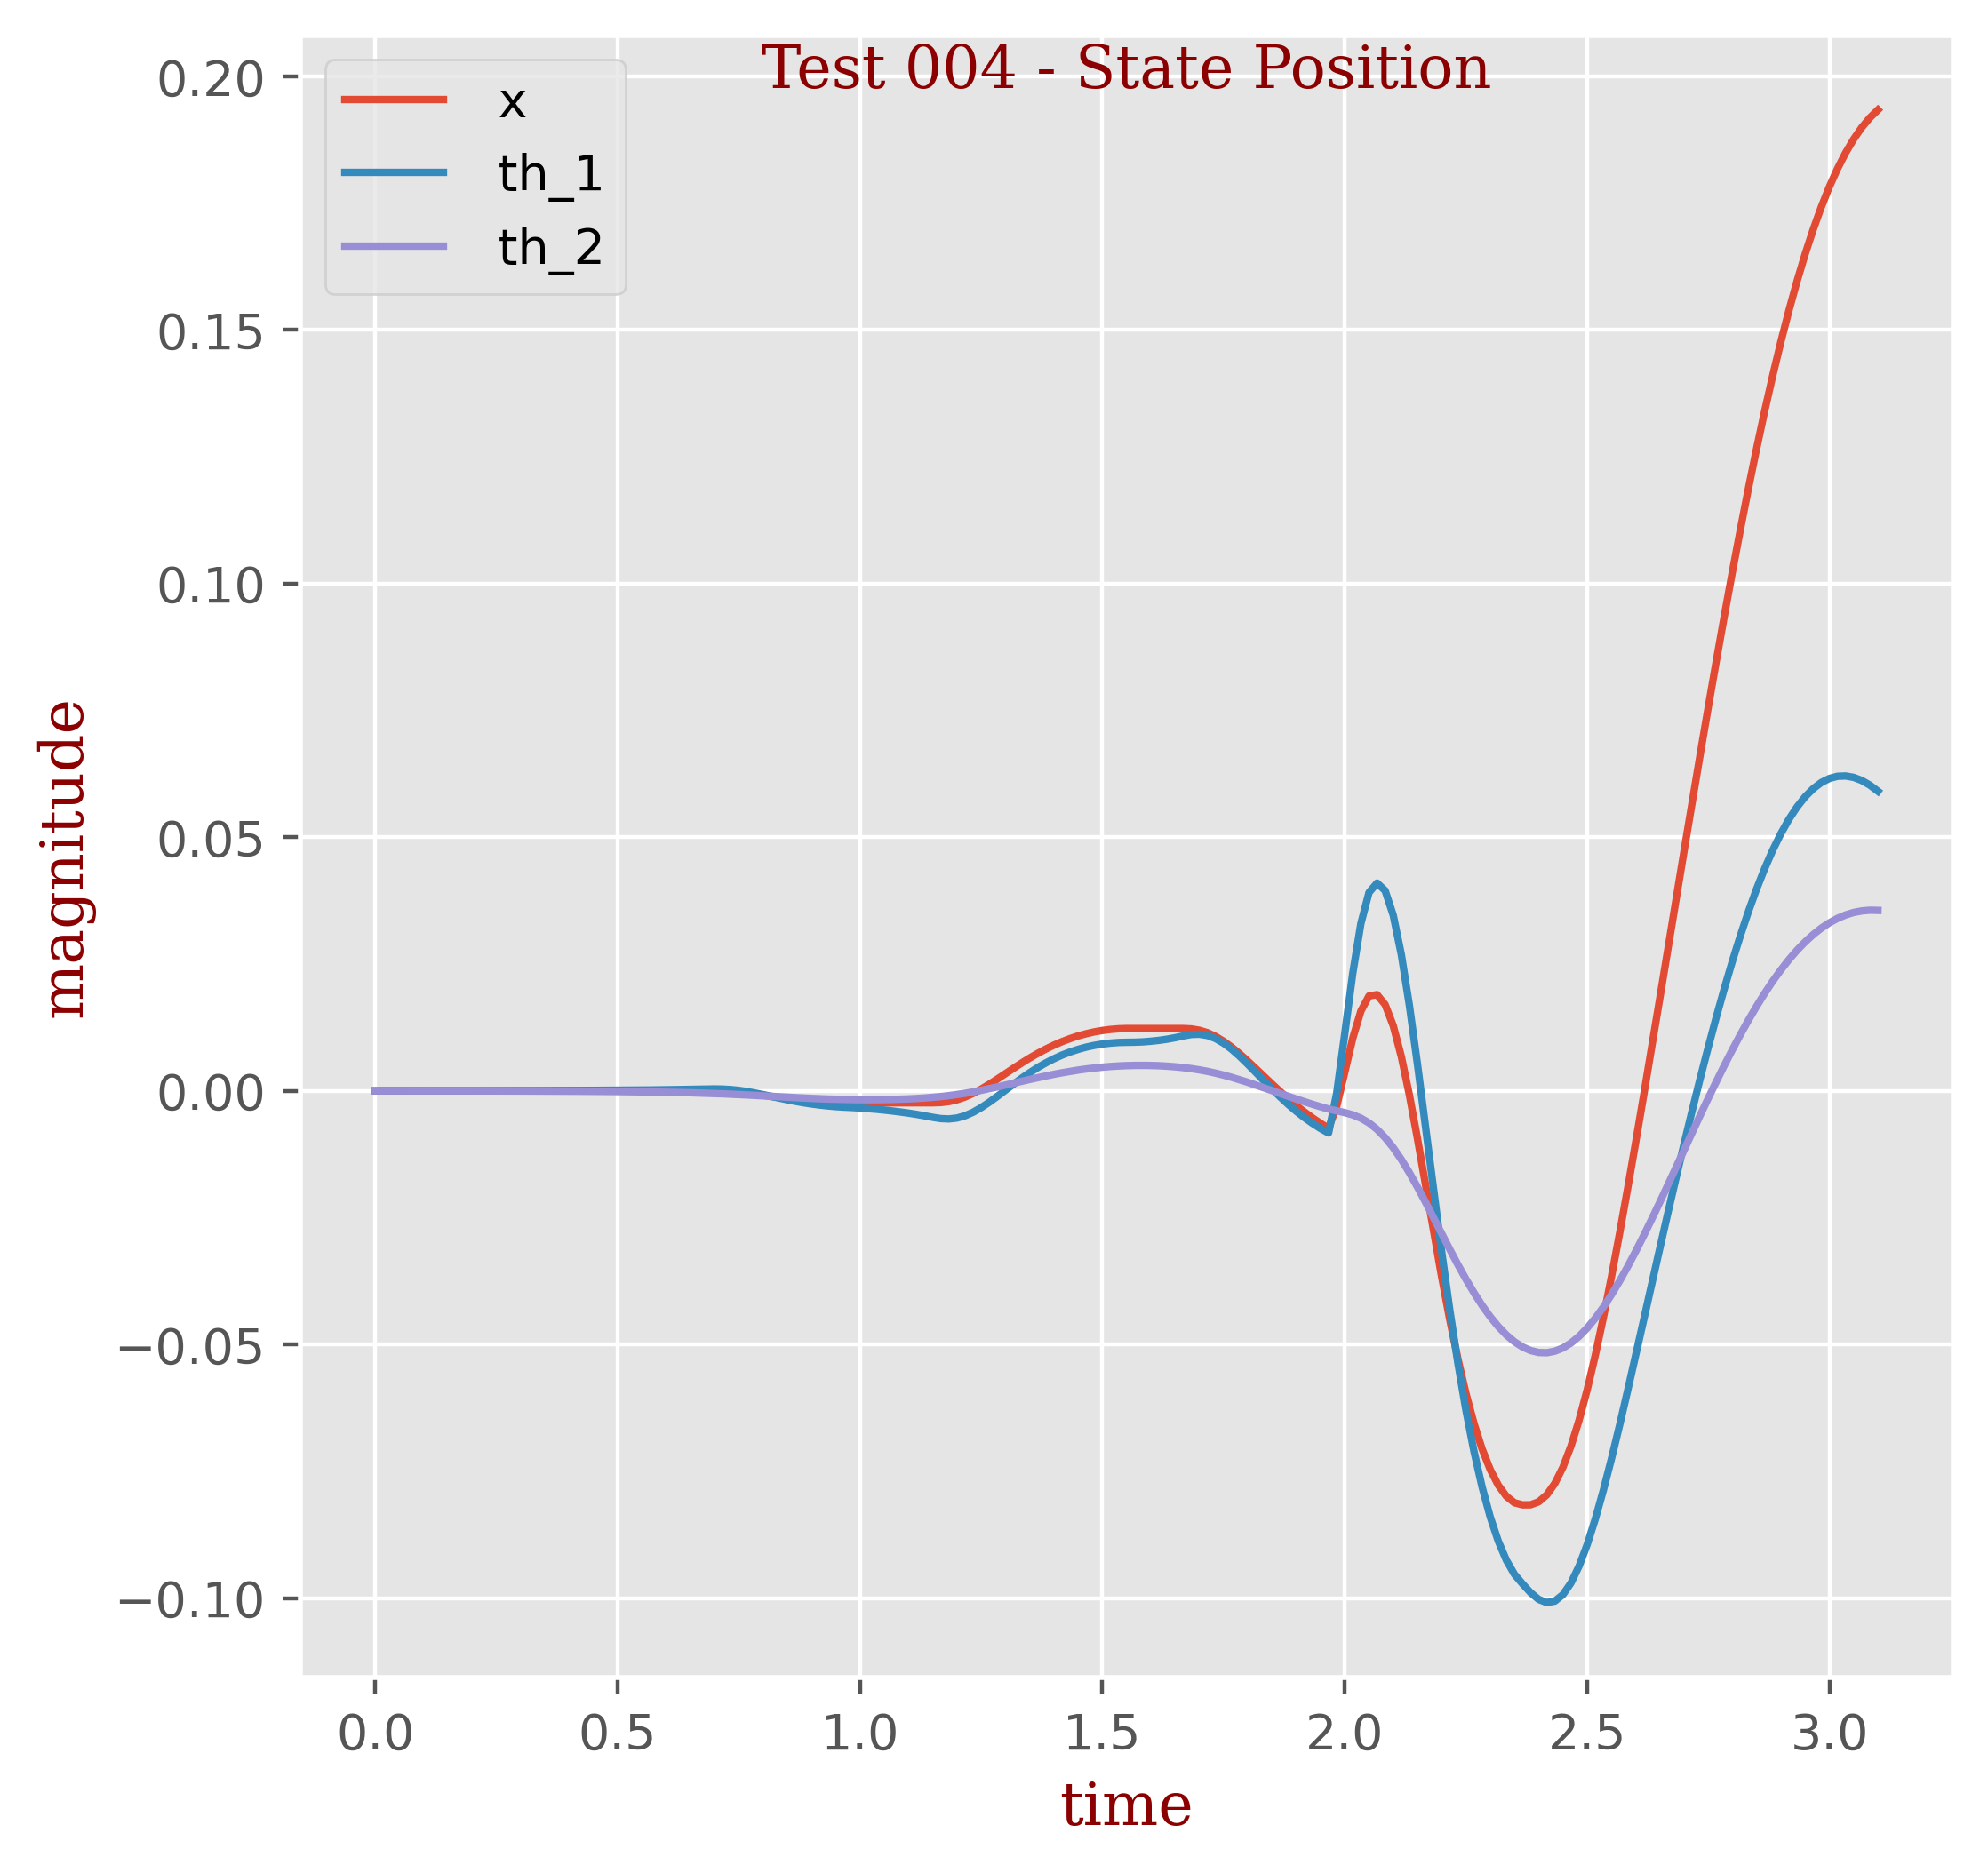
\includegraphics[width=27mm]{Test 004_State_Position.png}}
\subfigure[\(\dot{q}(t)\)]{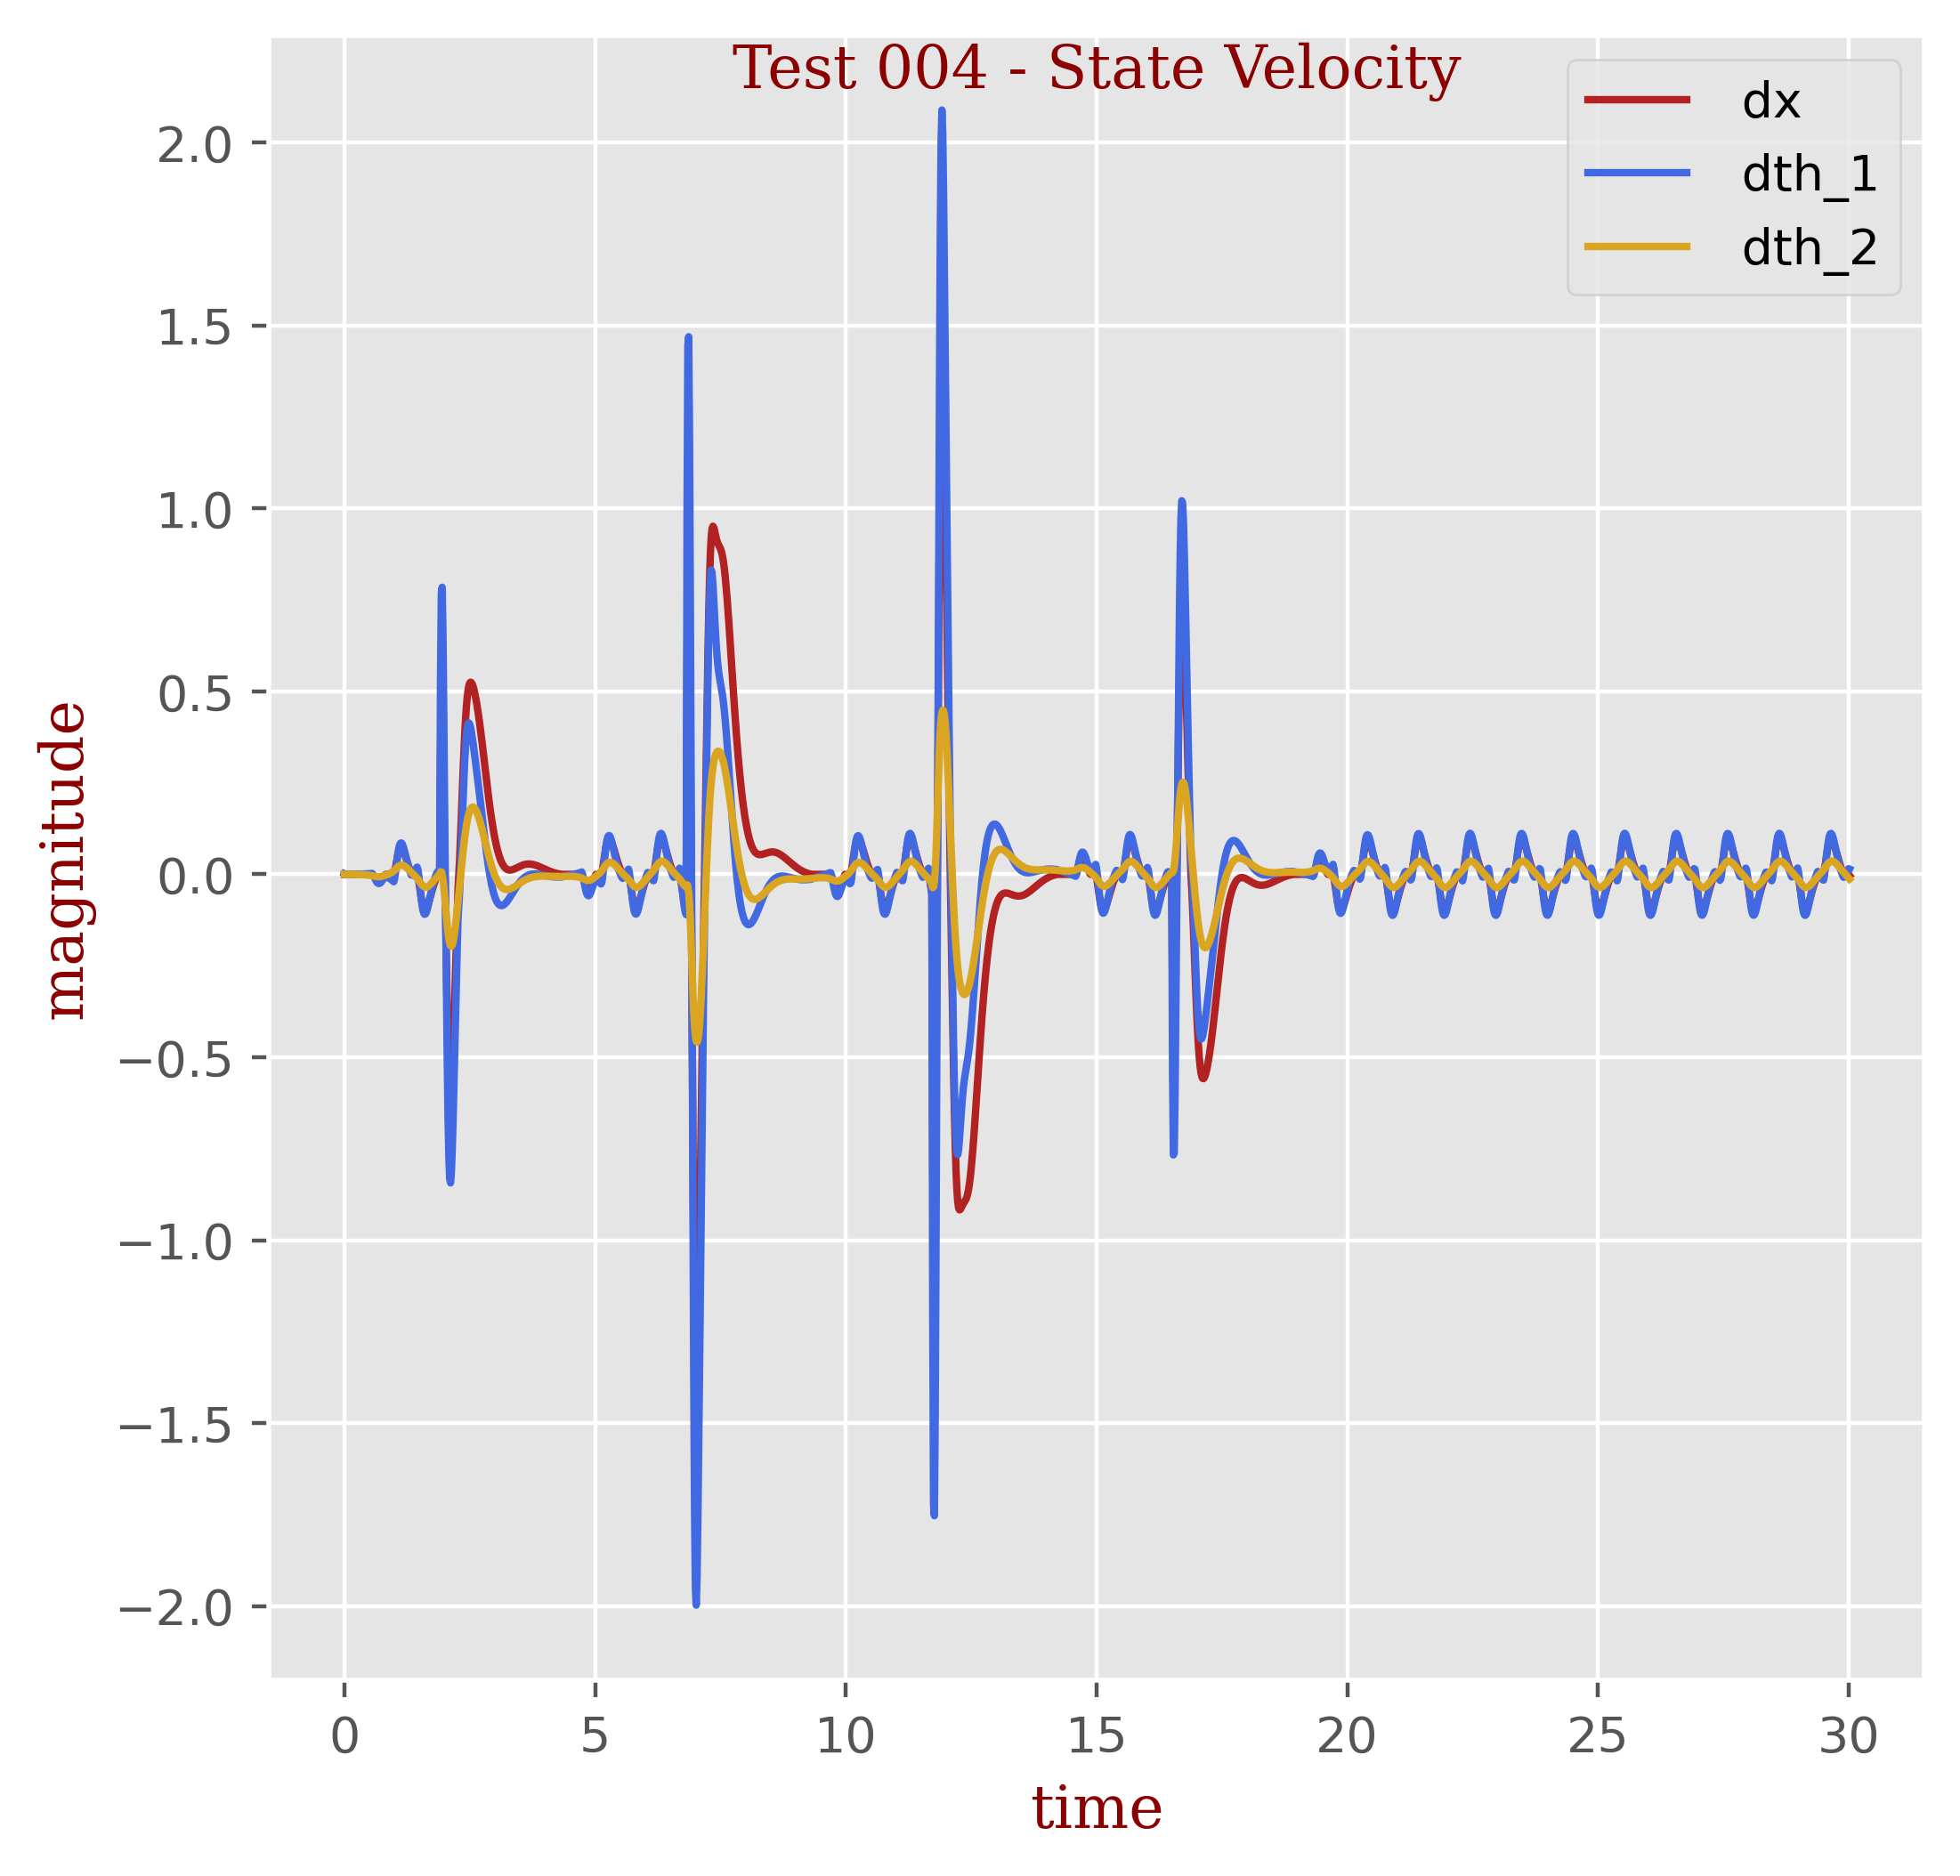
\includegraphics[width=27mm]{Test 004_State_Velocity.png}}
      \subfigure[\(J(t)\)]{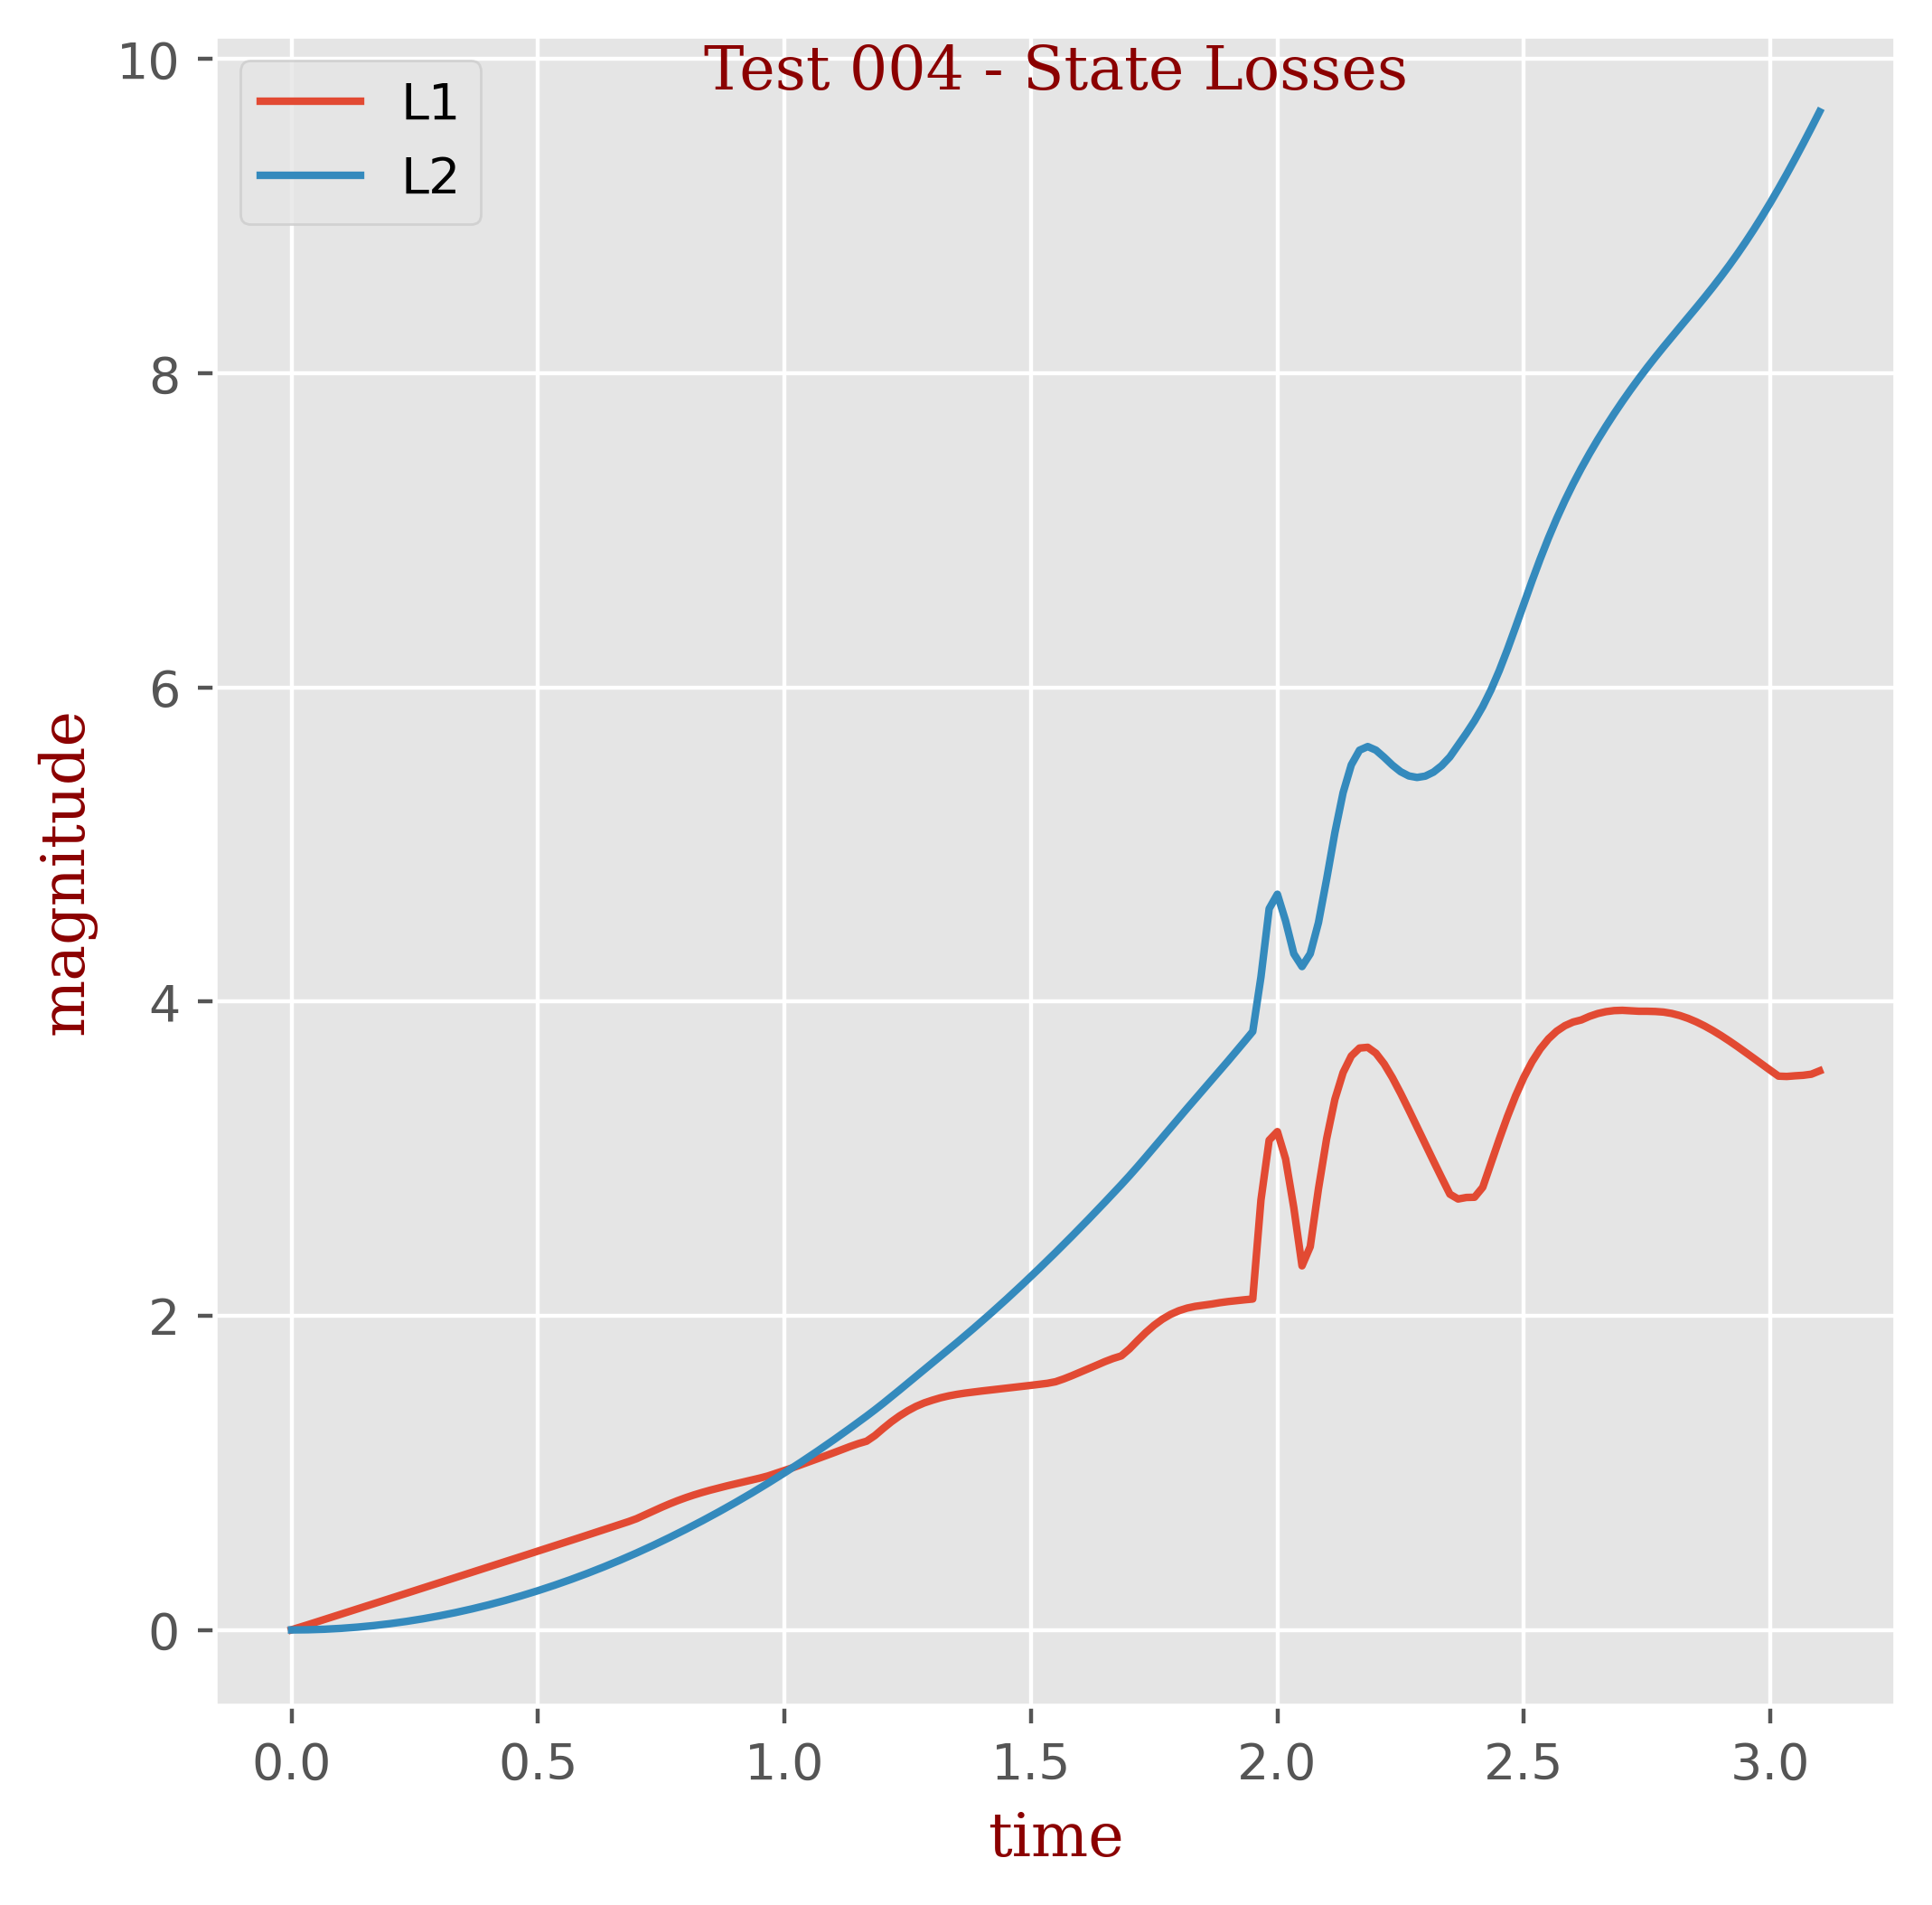
\includegraphics[width=27mm]{Test 004_State_Losses.png}}
\caption{Test 004}
\label{fig:t004}
\end{figure}

\begin{figure}
\centering
      \subfigure[\(q(t)\)]{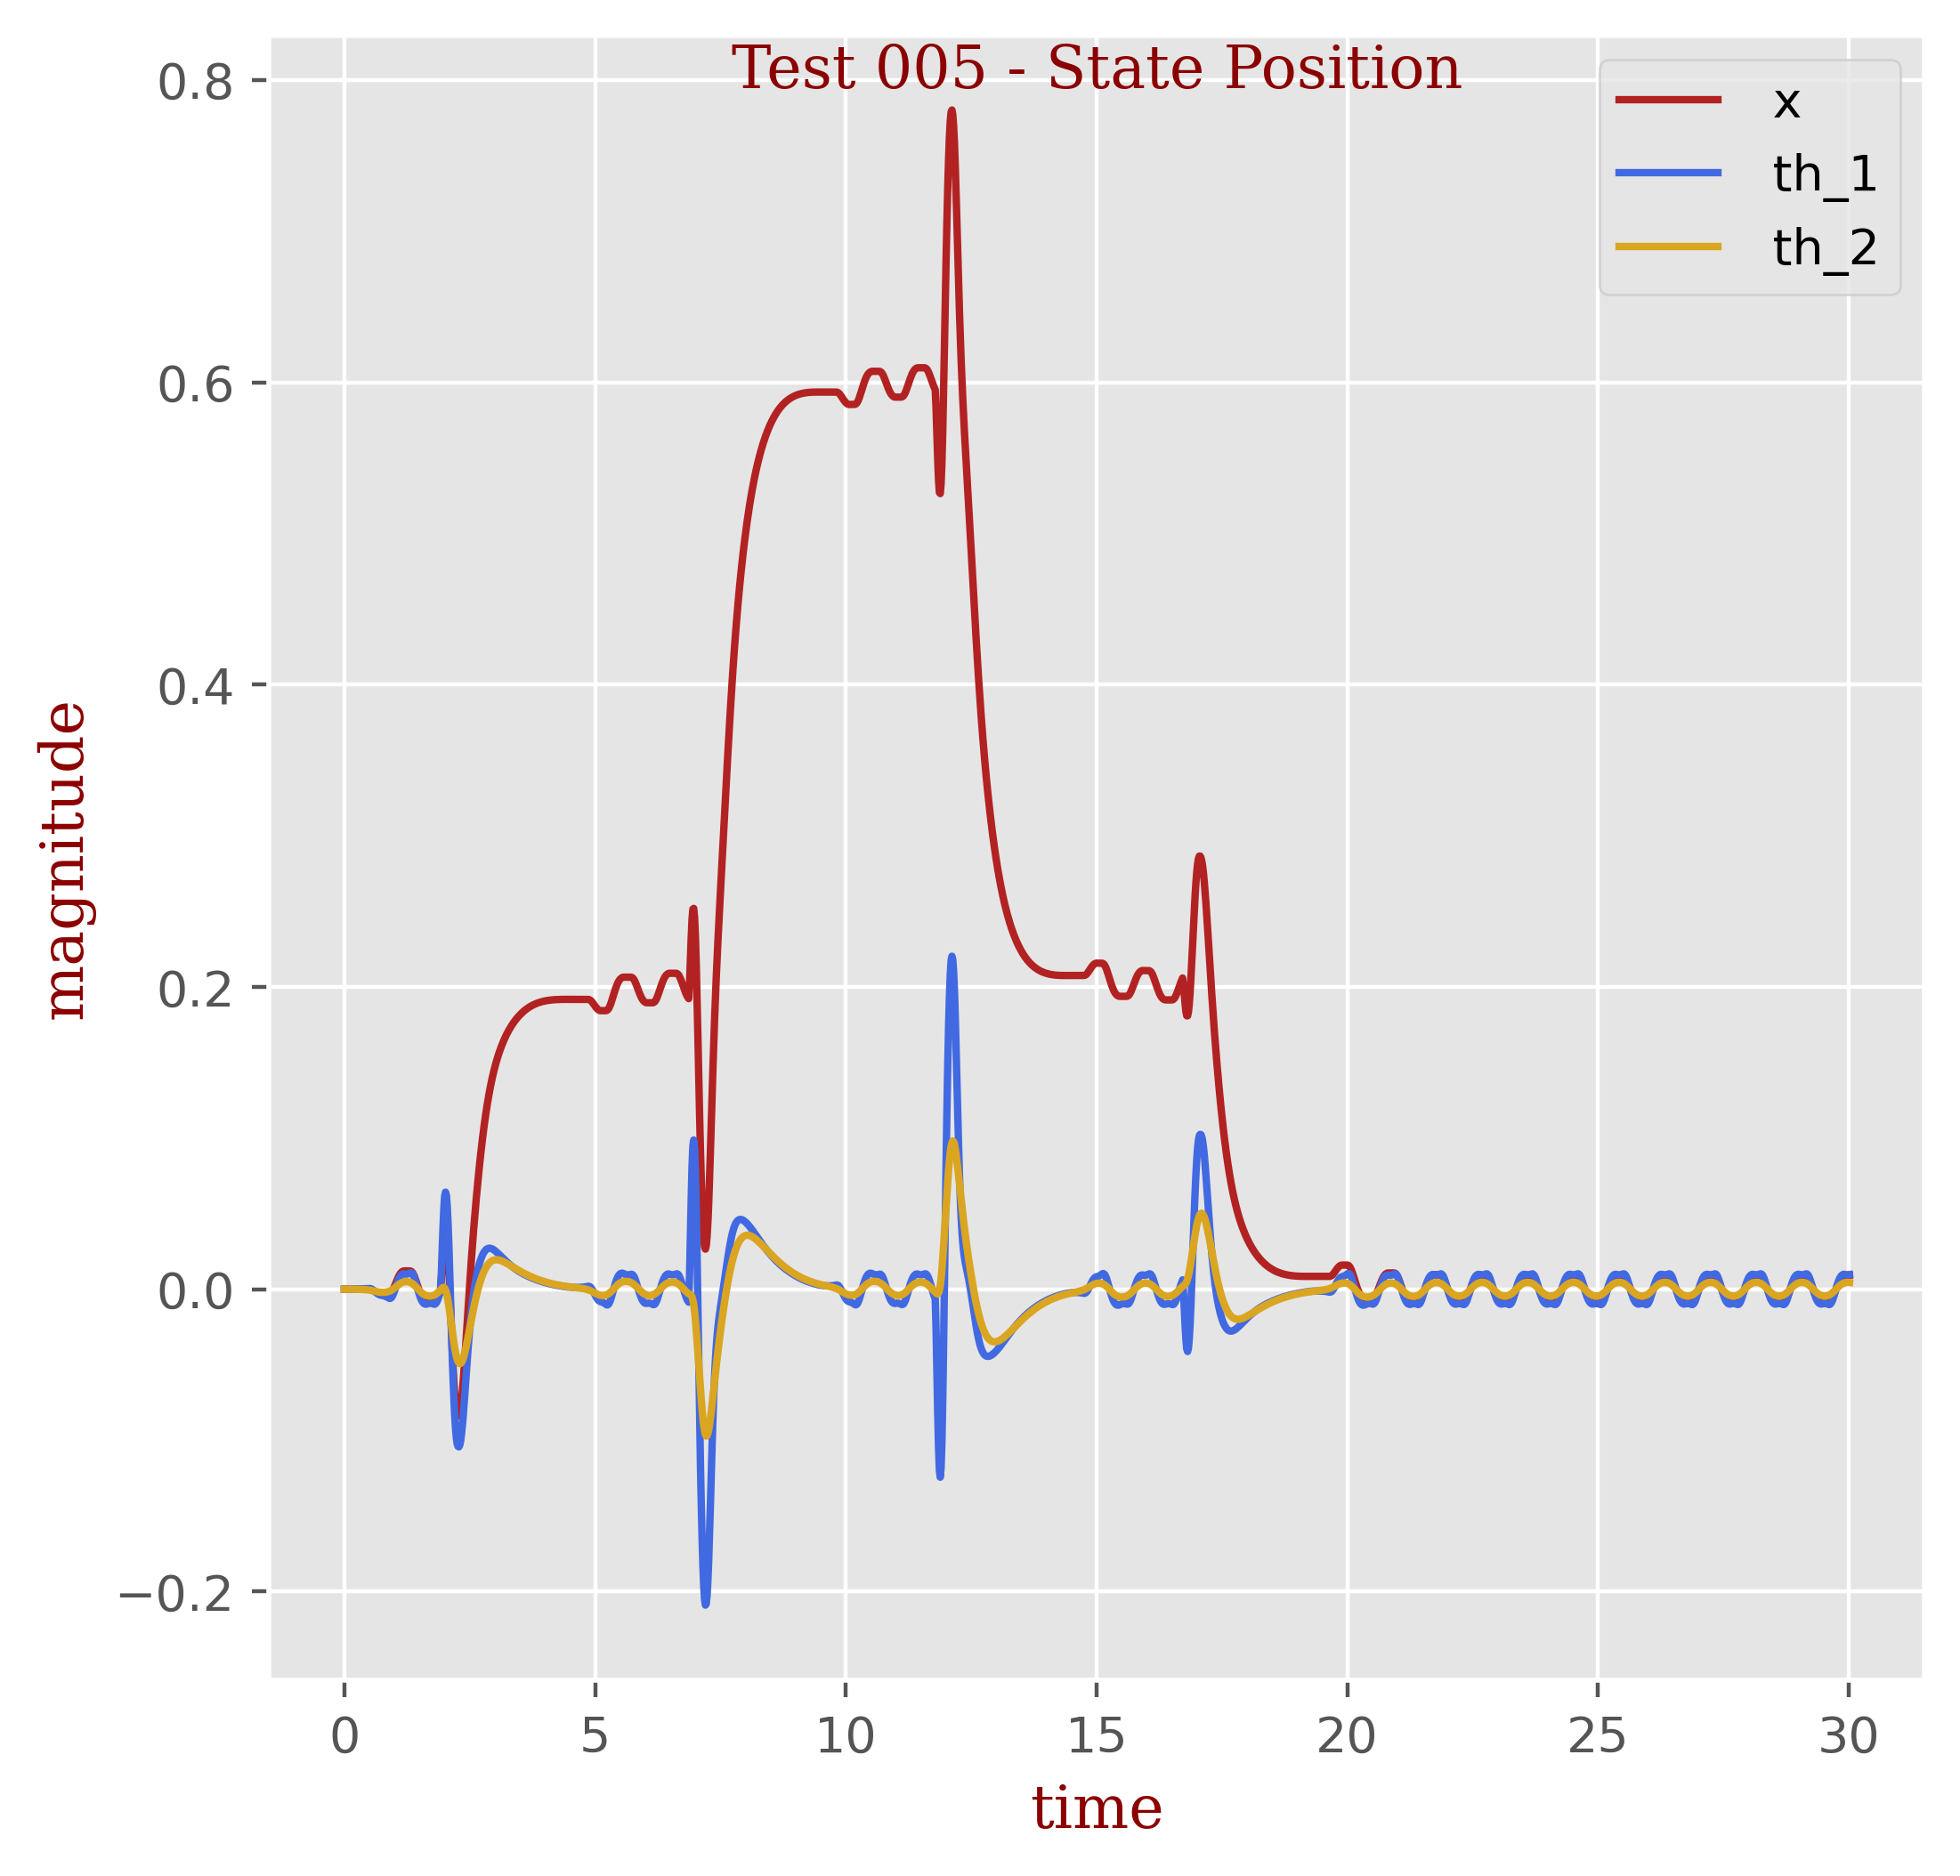
\includegraphics[width=27mm]{Test 005_State_Position.png}}
\subfigure[\(\dot{q}(t)\)]{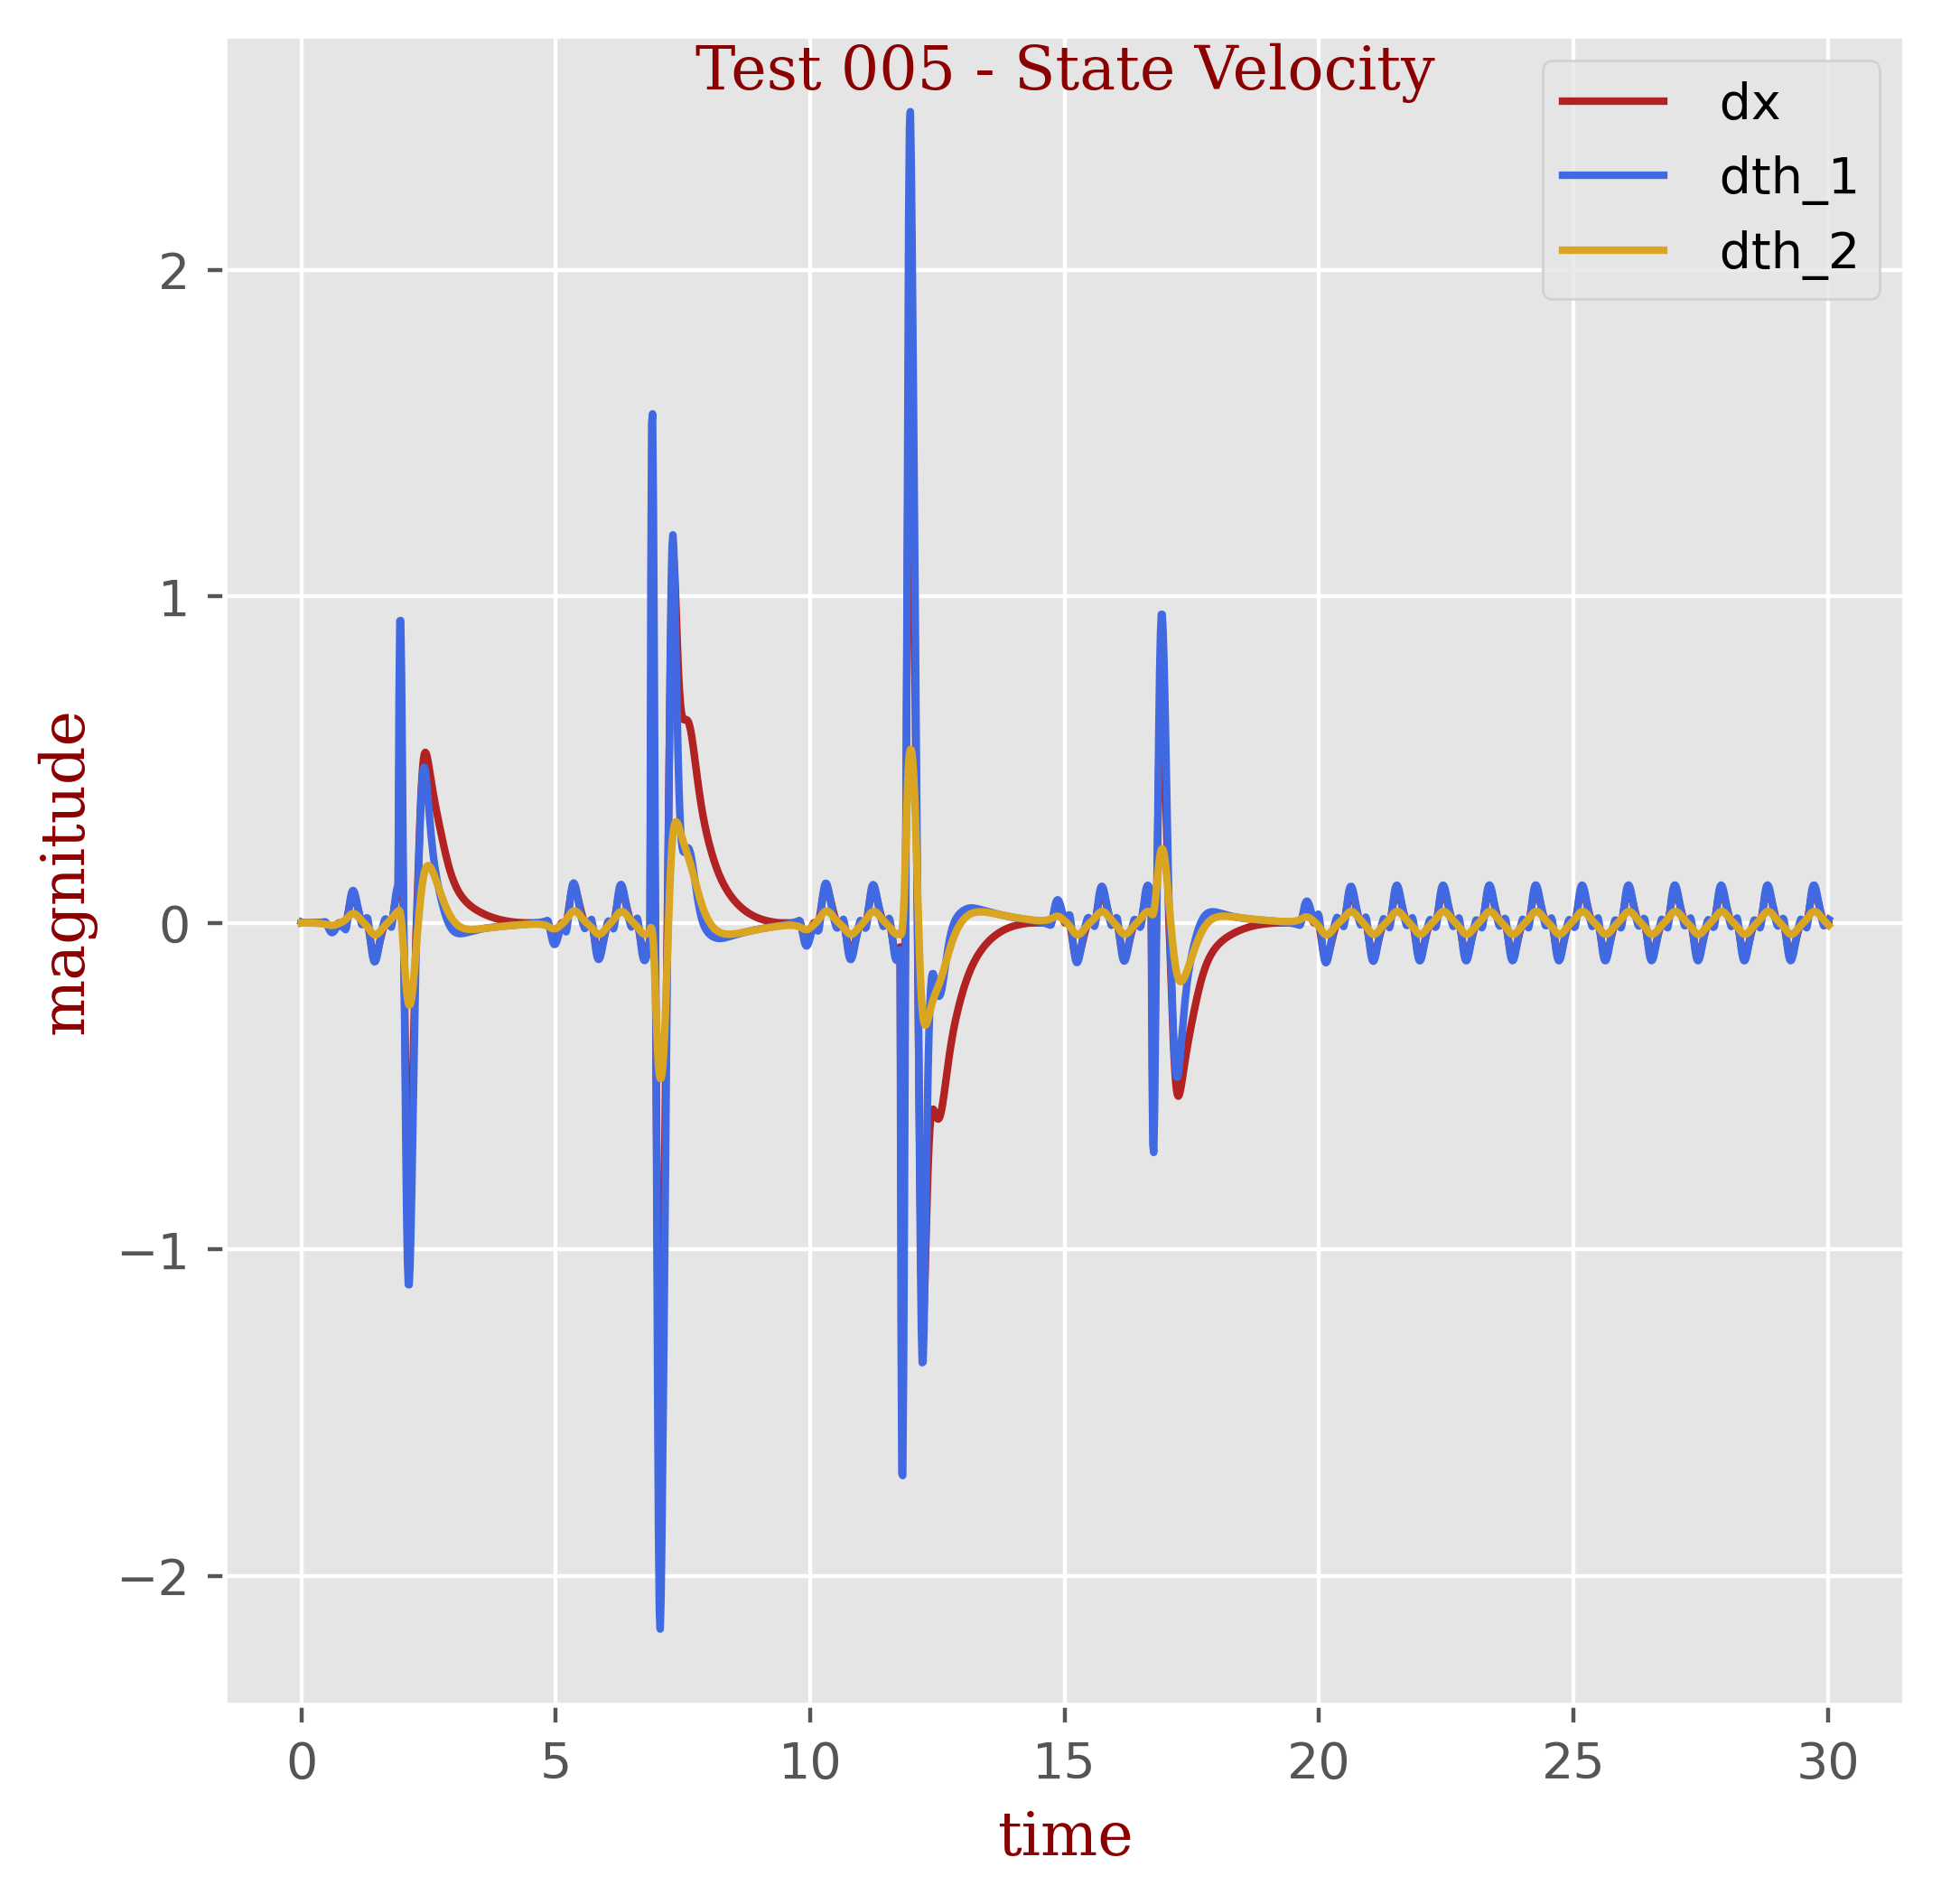
\includegraphics[width=27mm]{Test 005_State_Velocity.png}}
      \subfigure[\(J(t)\)]{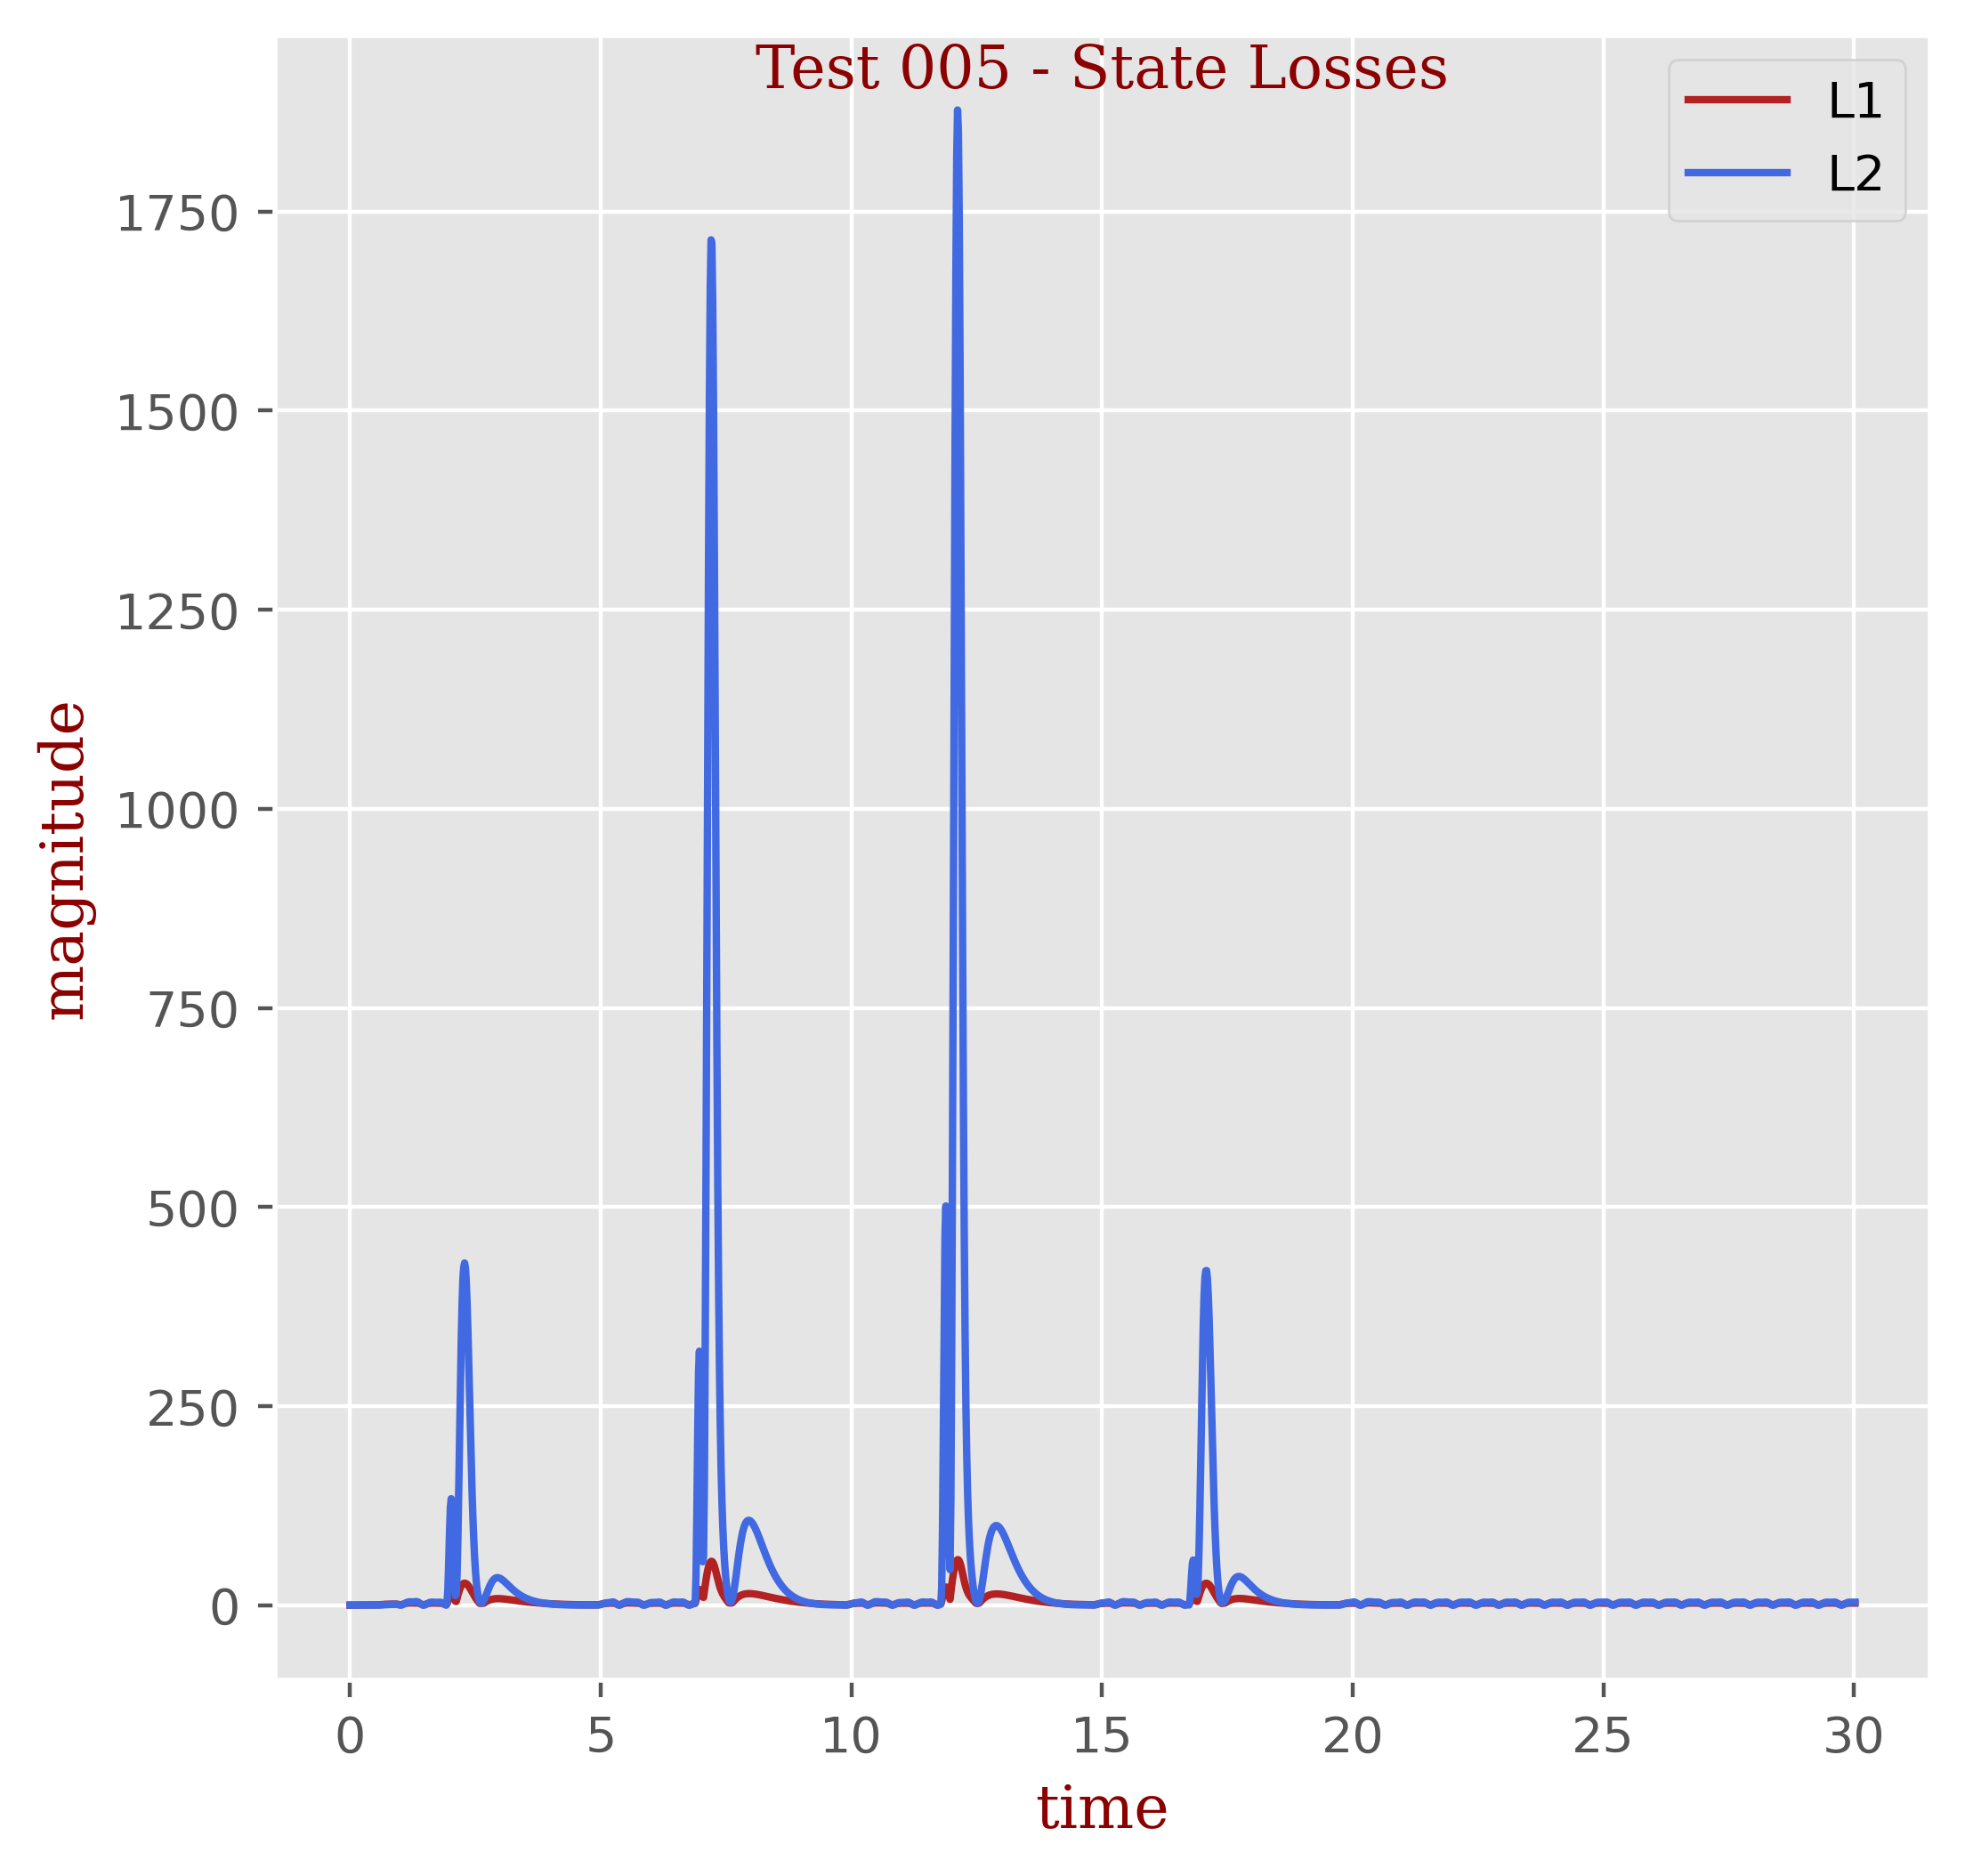
\includegraphics[width=27mm]{Test 005_State_Losses.png}}
\caption{Test 005}
\label{fig:t005}
\end{figure}

\begin{figure}
\centering
      \subfigure[\(q(t)\)]{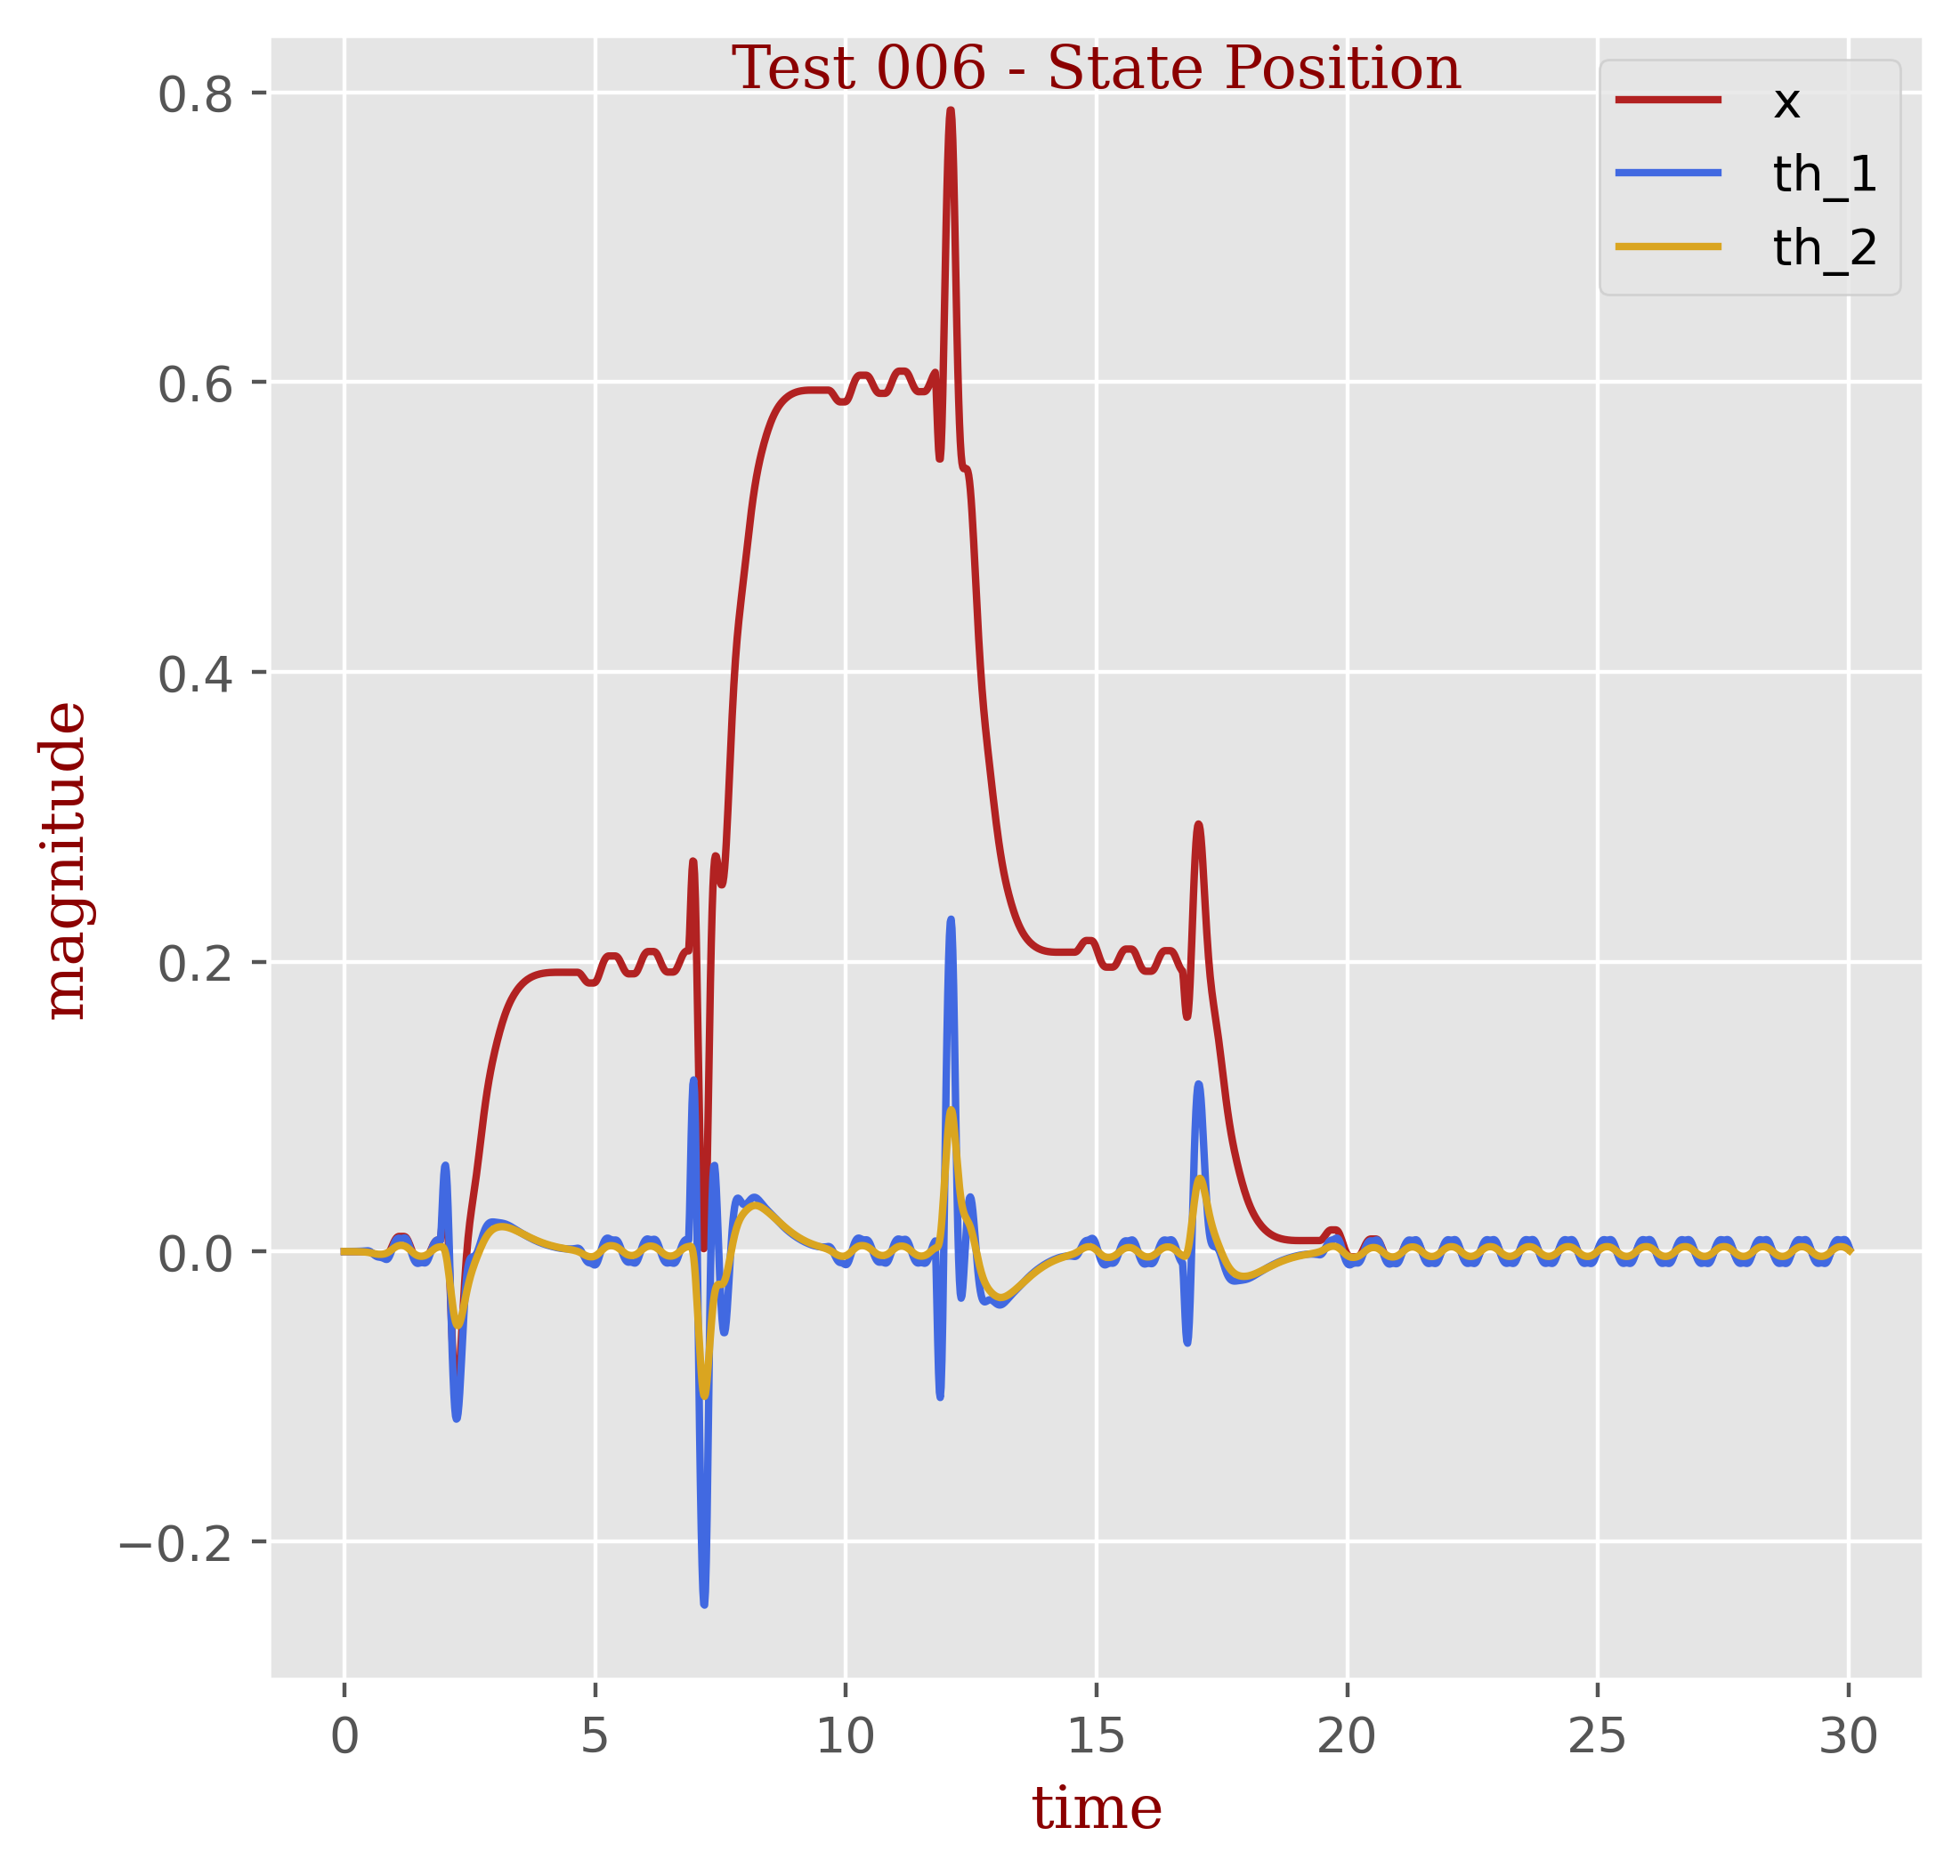
\includegraphics[width=27mm]{Test 006_State_Position.png}}
\subfigure[\(\dot{q}(t)\)]{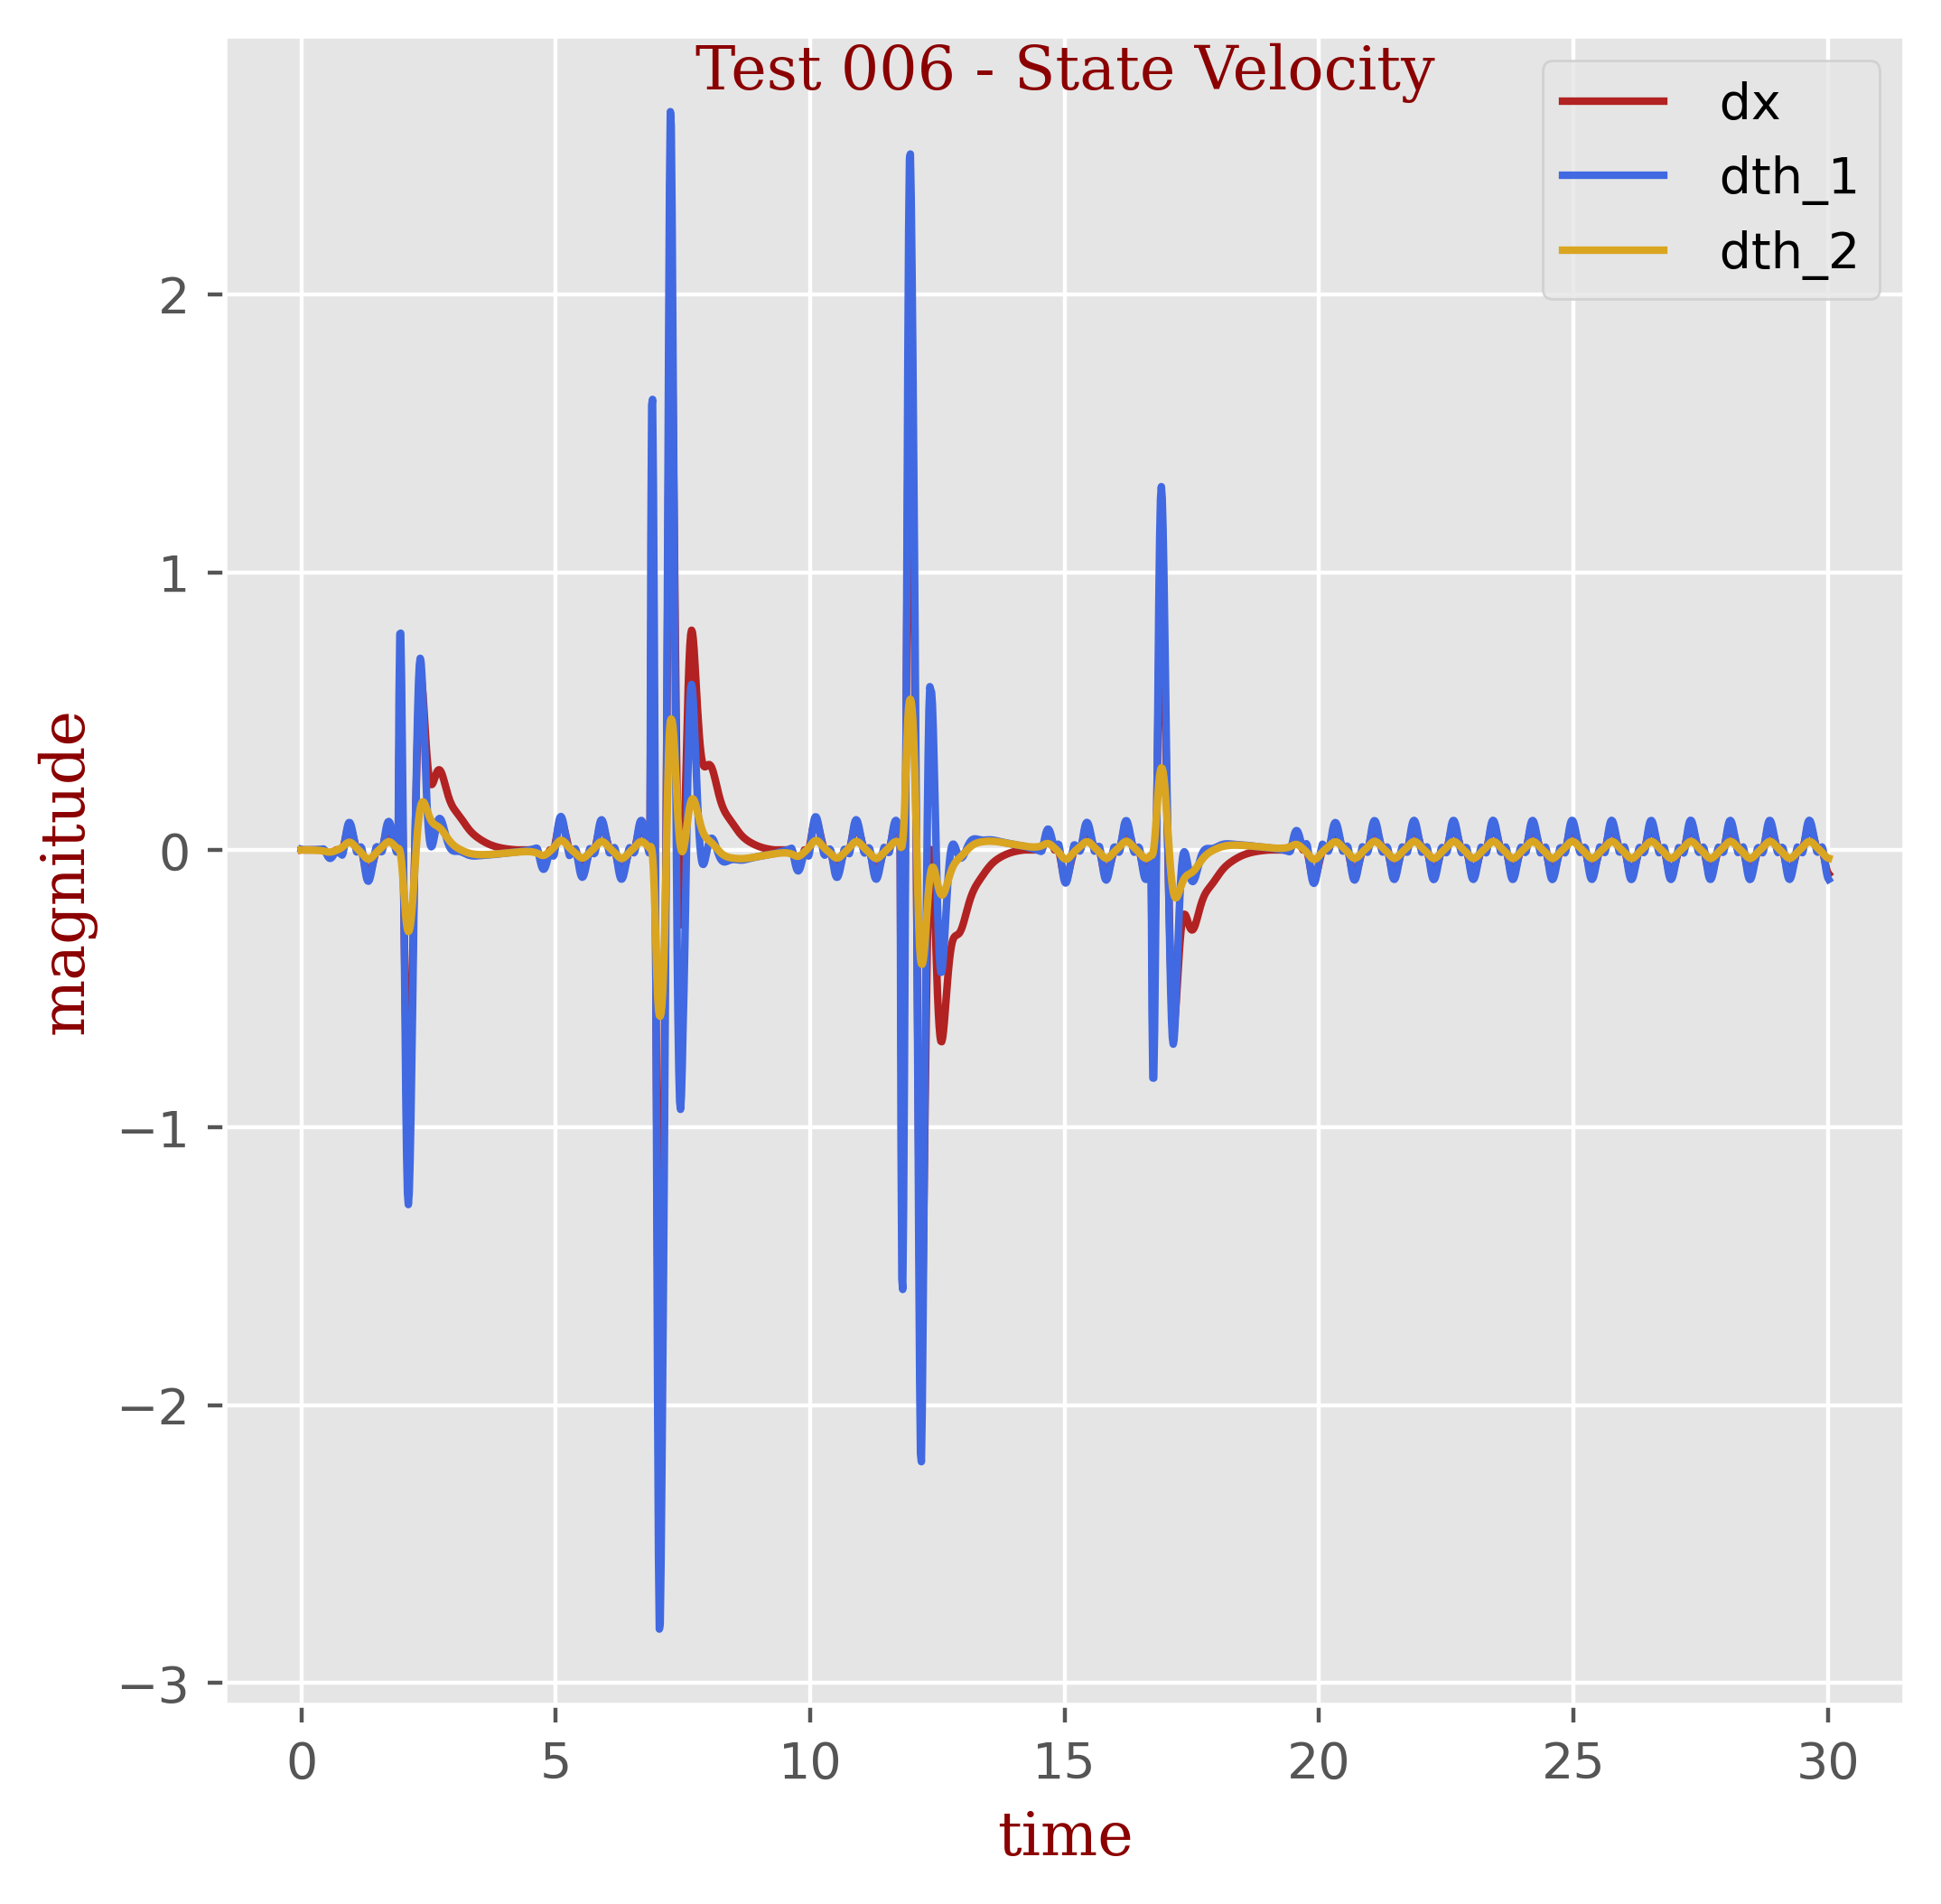
\includegraphics[width=27mm]{Test 006_State_Velocity.png}}
      \subfigure[\(J(t)\)]{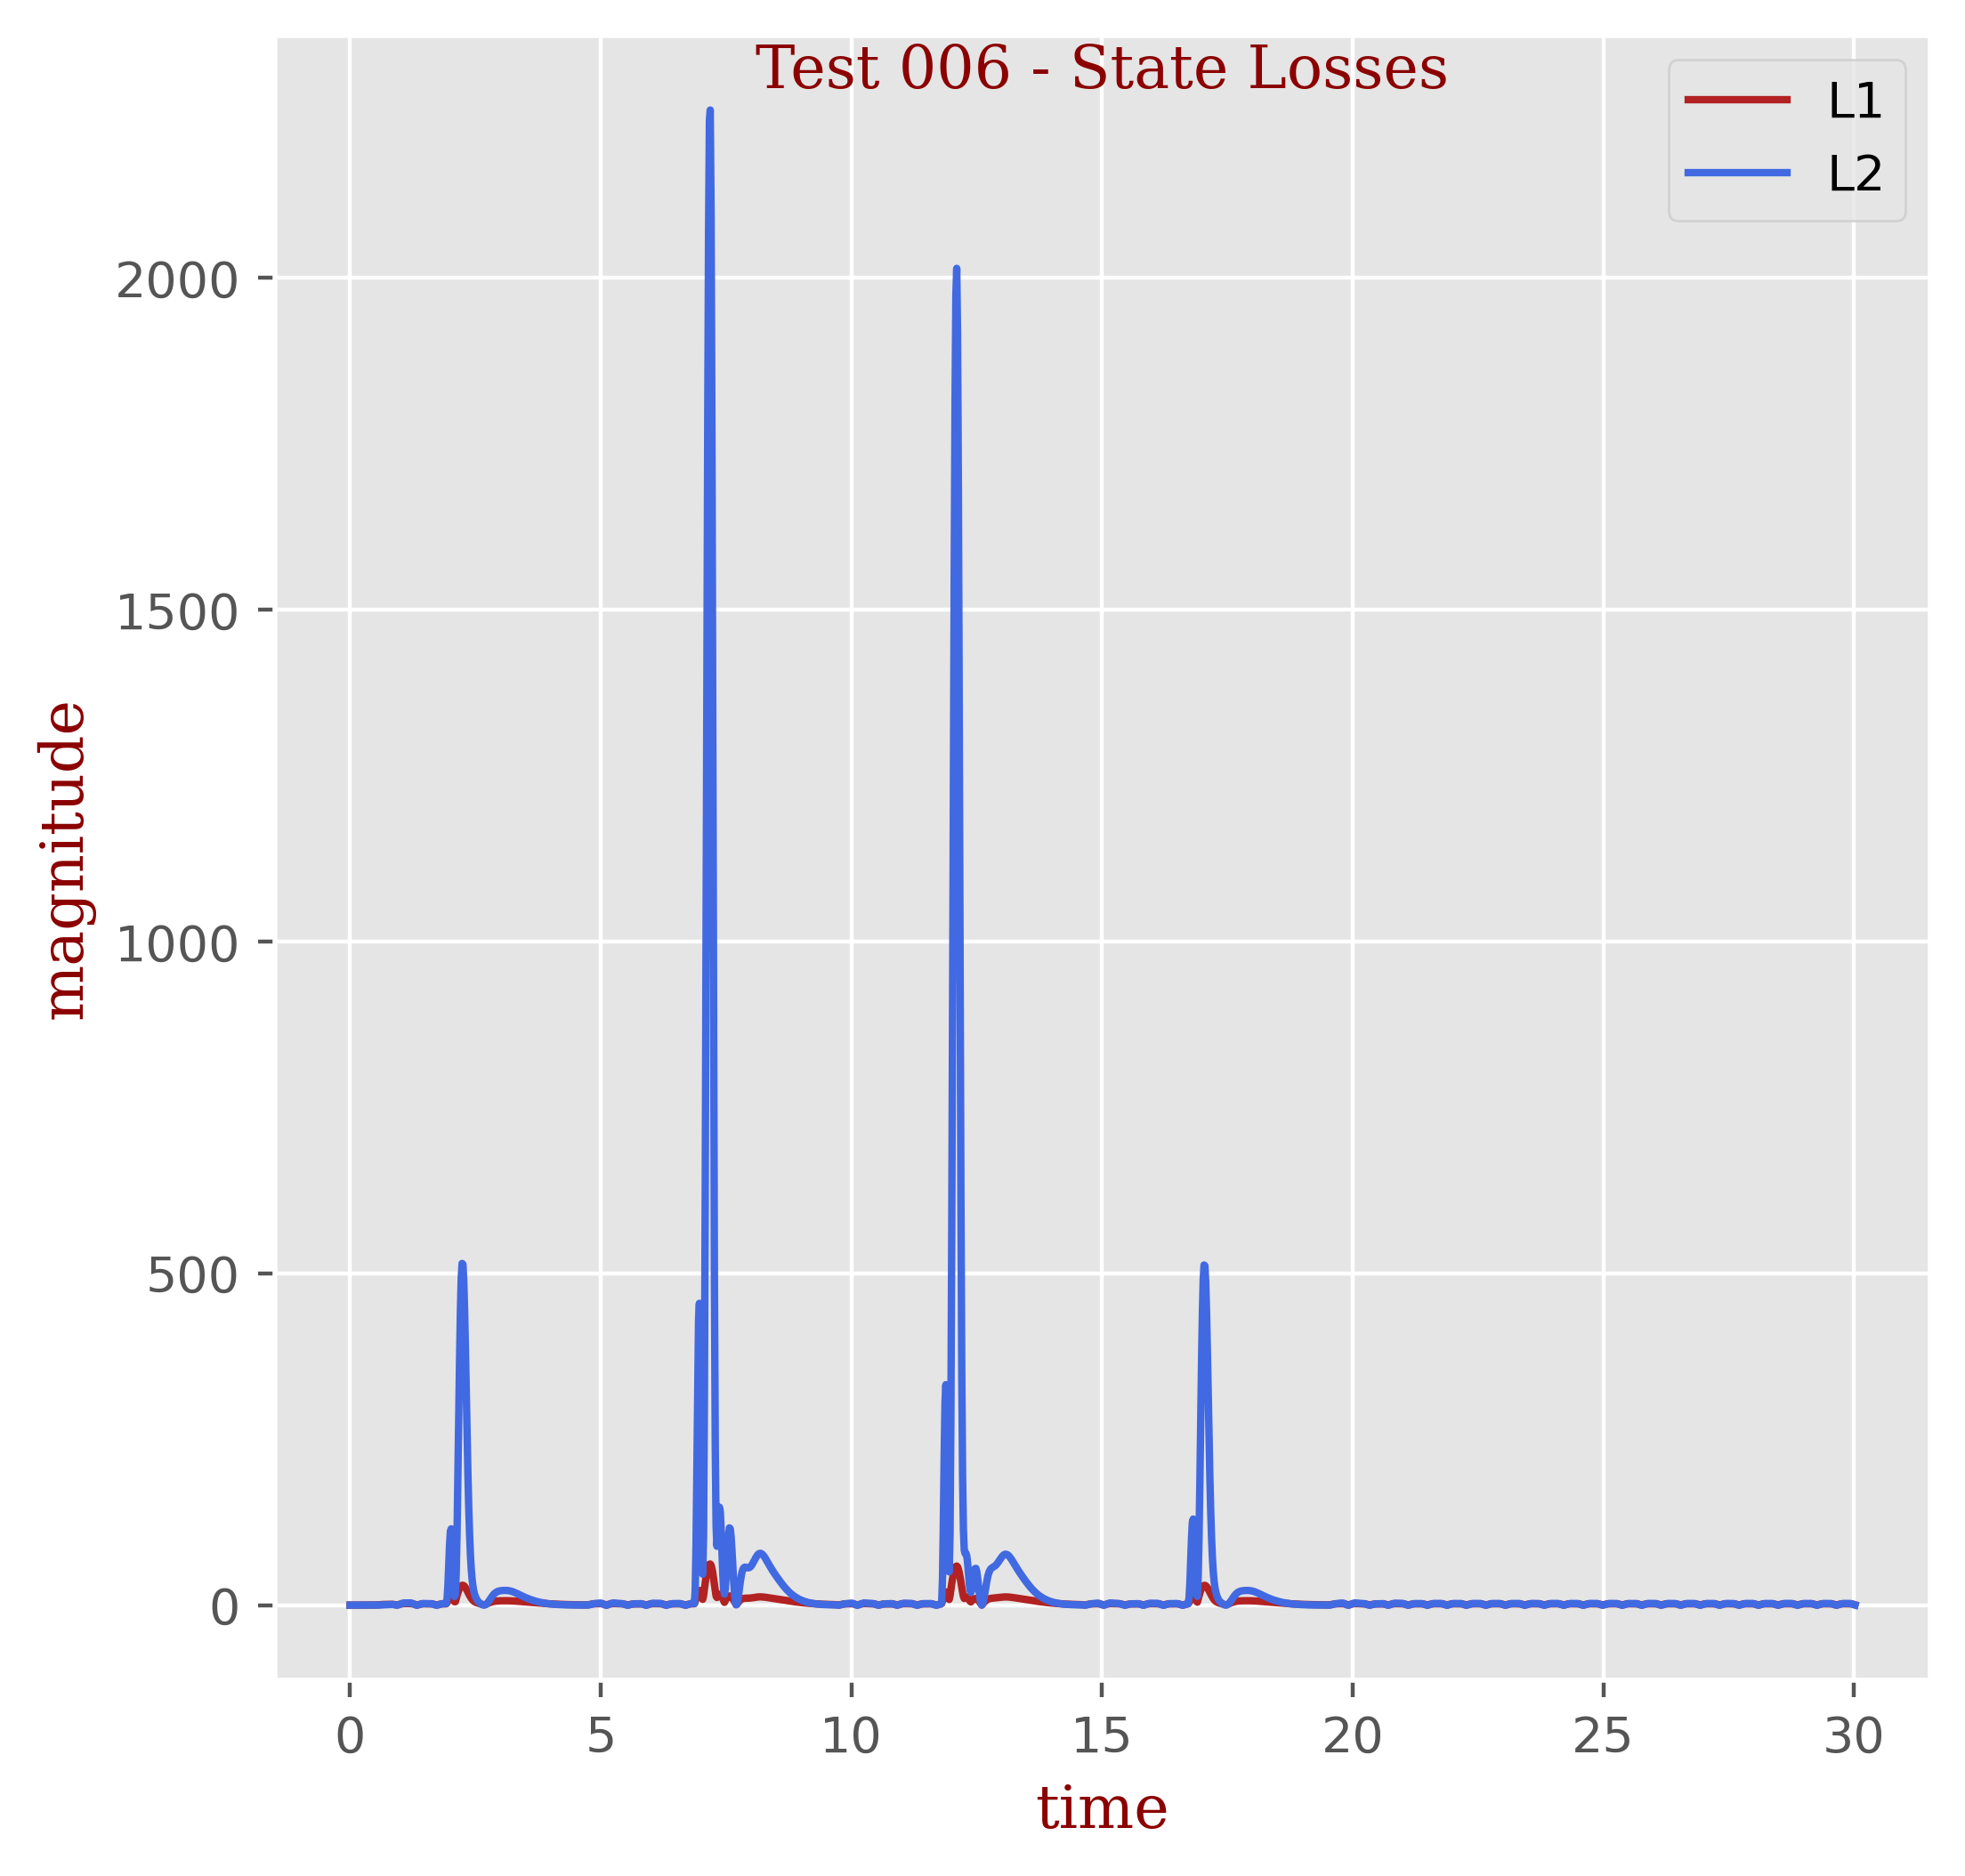
\includegraphics[width=27mm]{Test 006_State_Losses.png}}
\caption{Test 005}
\label{fig:t005}
\end{figure}


\begin{figure}
\centering
      \subfigure[\(q(t)\)]{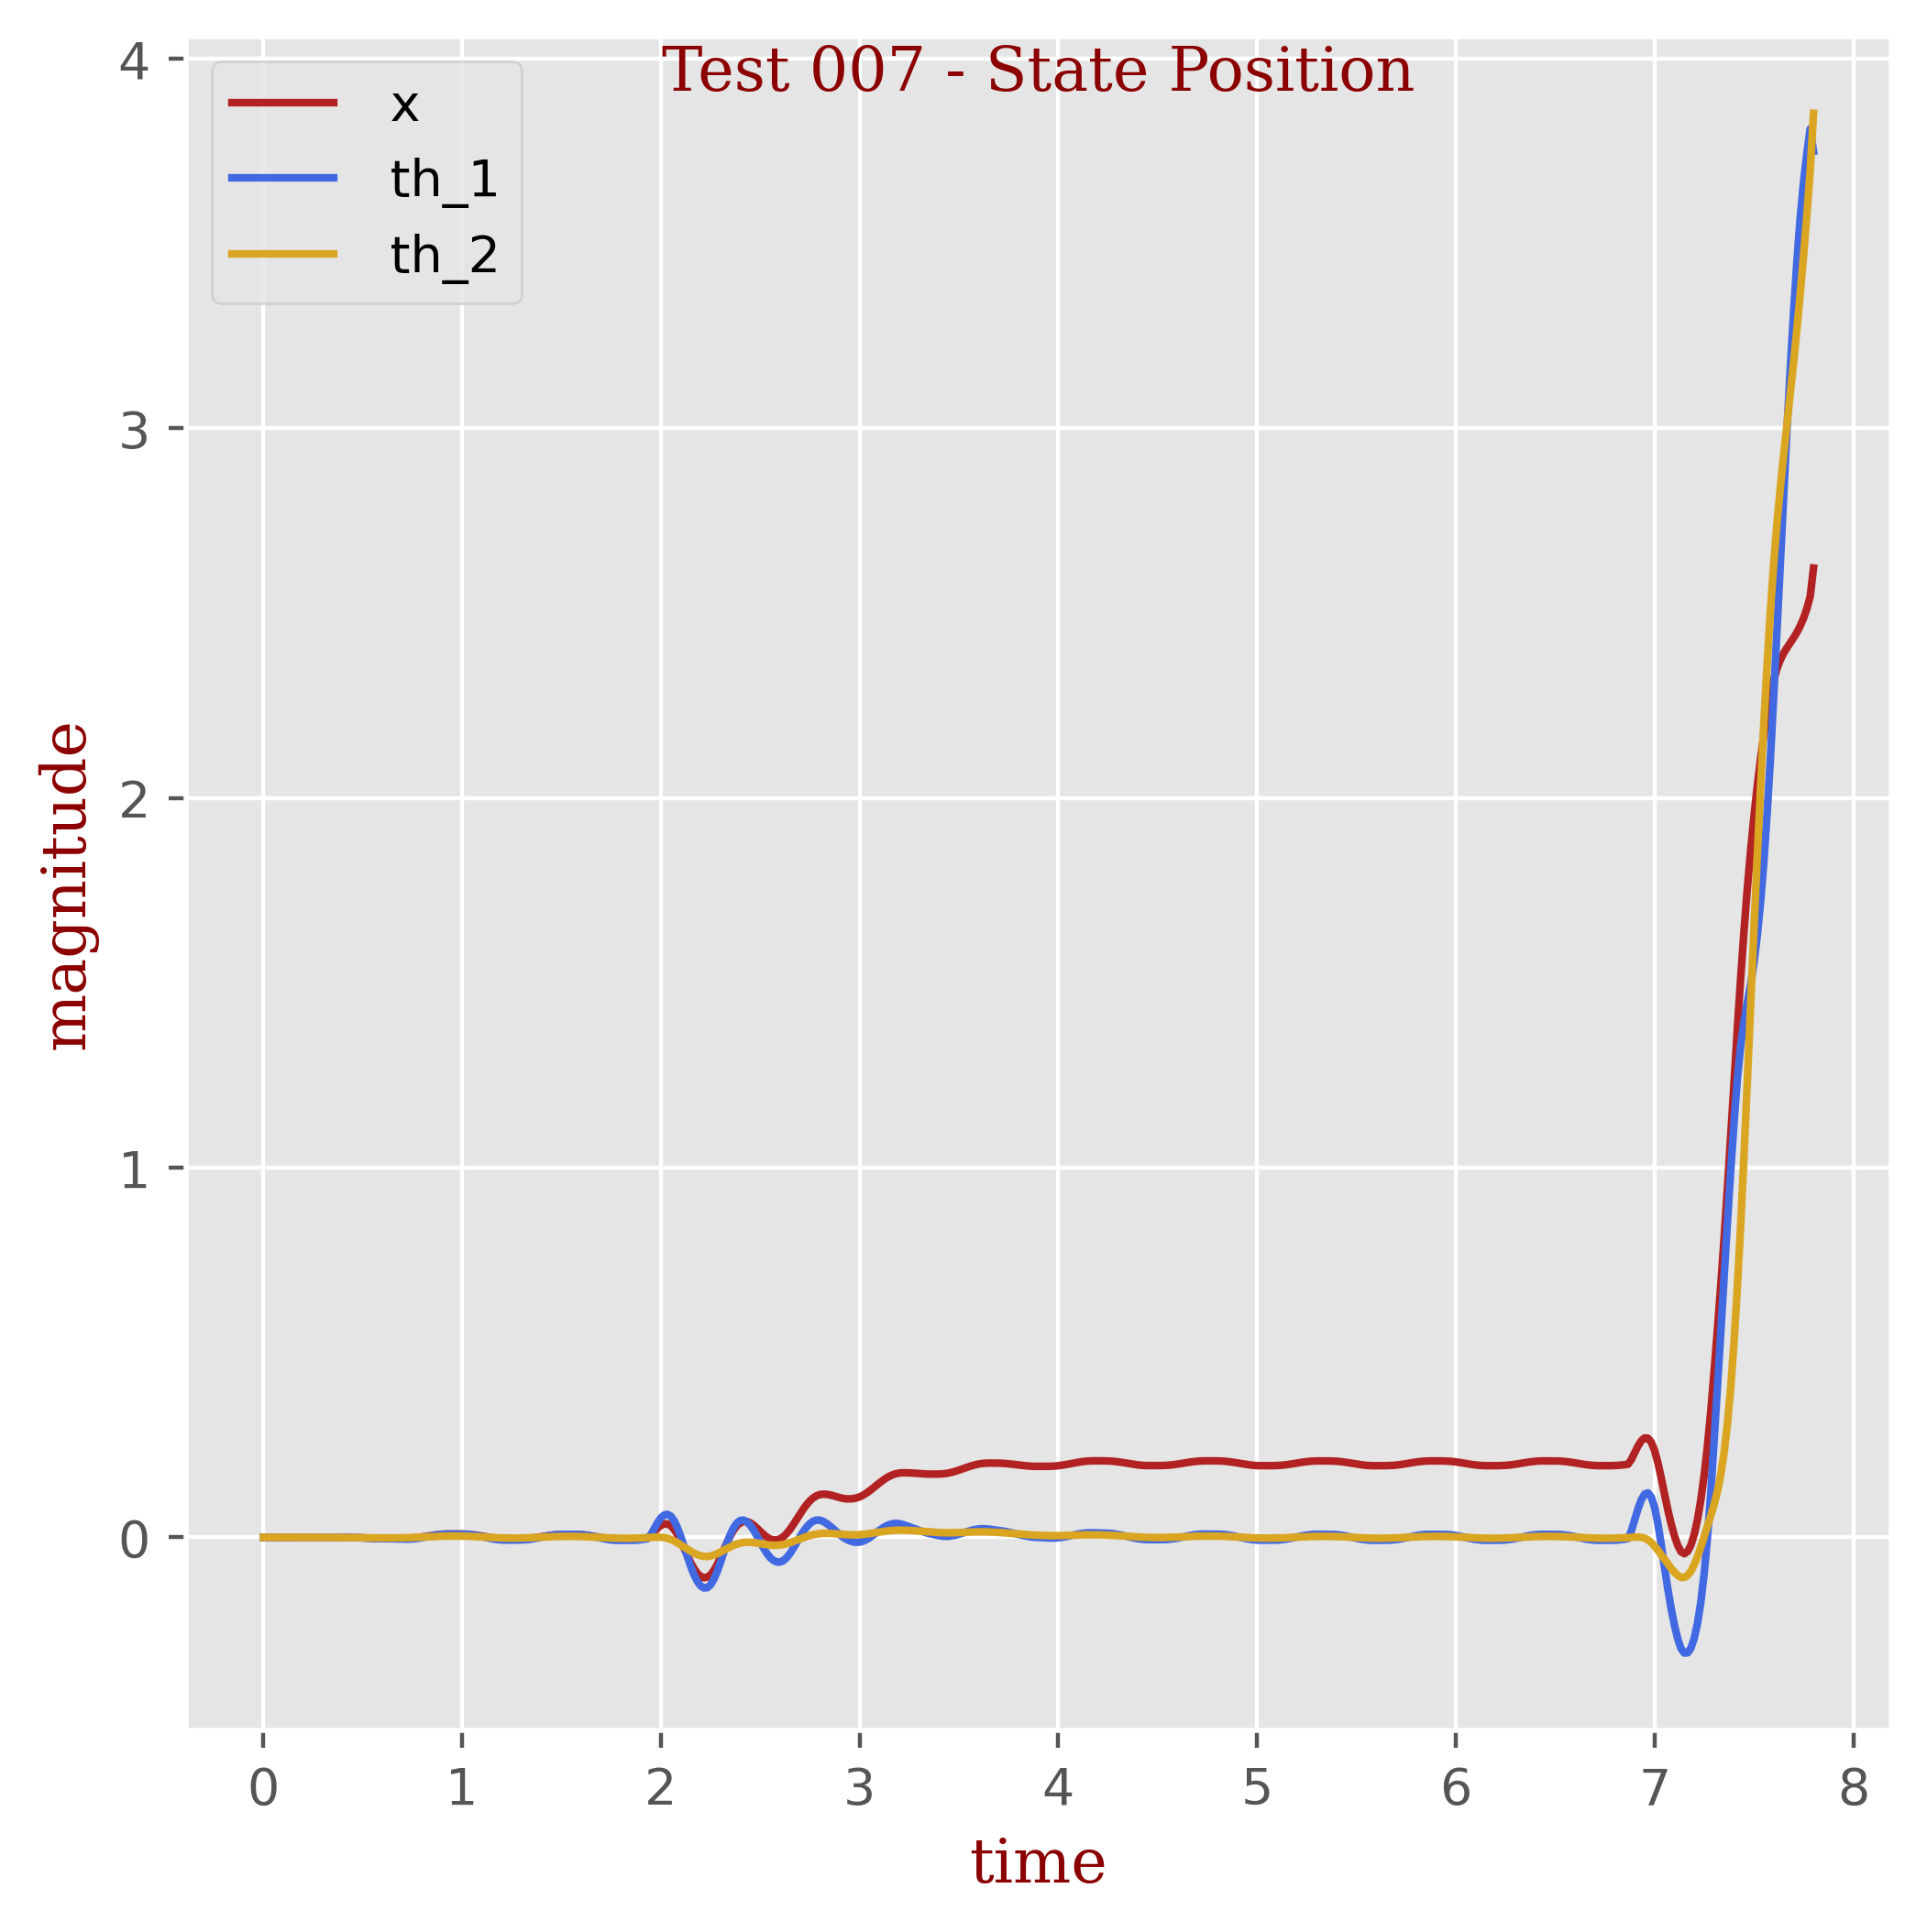
\includegraphics[width=27mm]{Test 007_State_Position.png}}
\subfigure[\(\dot{q}(t)\)]{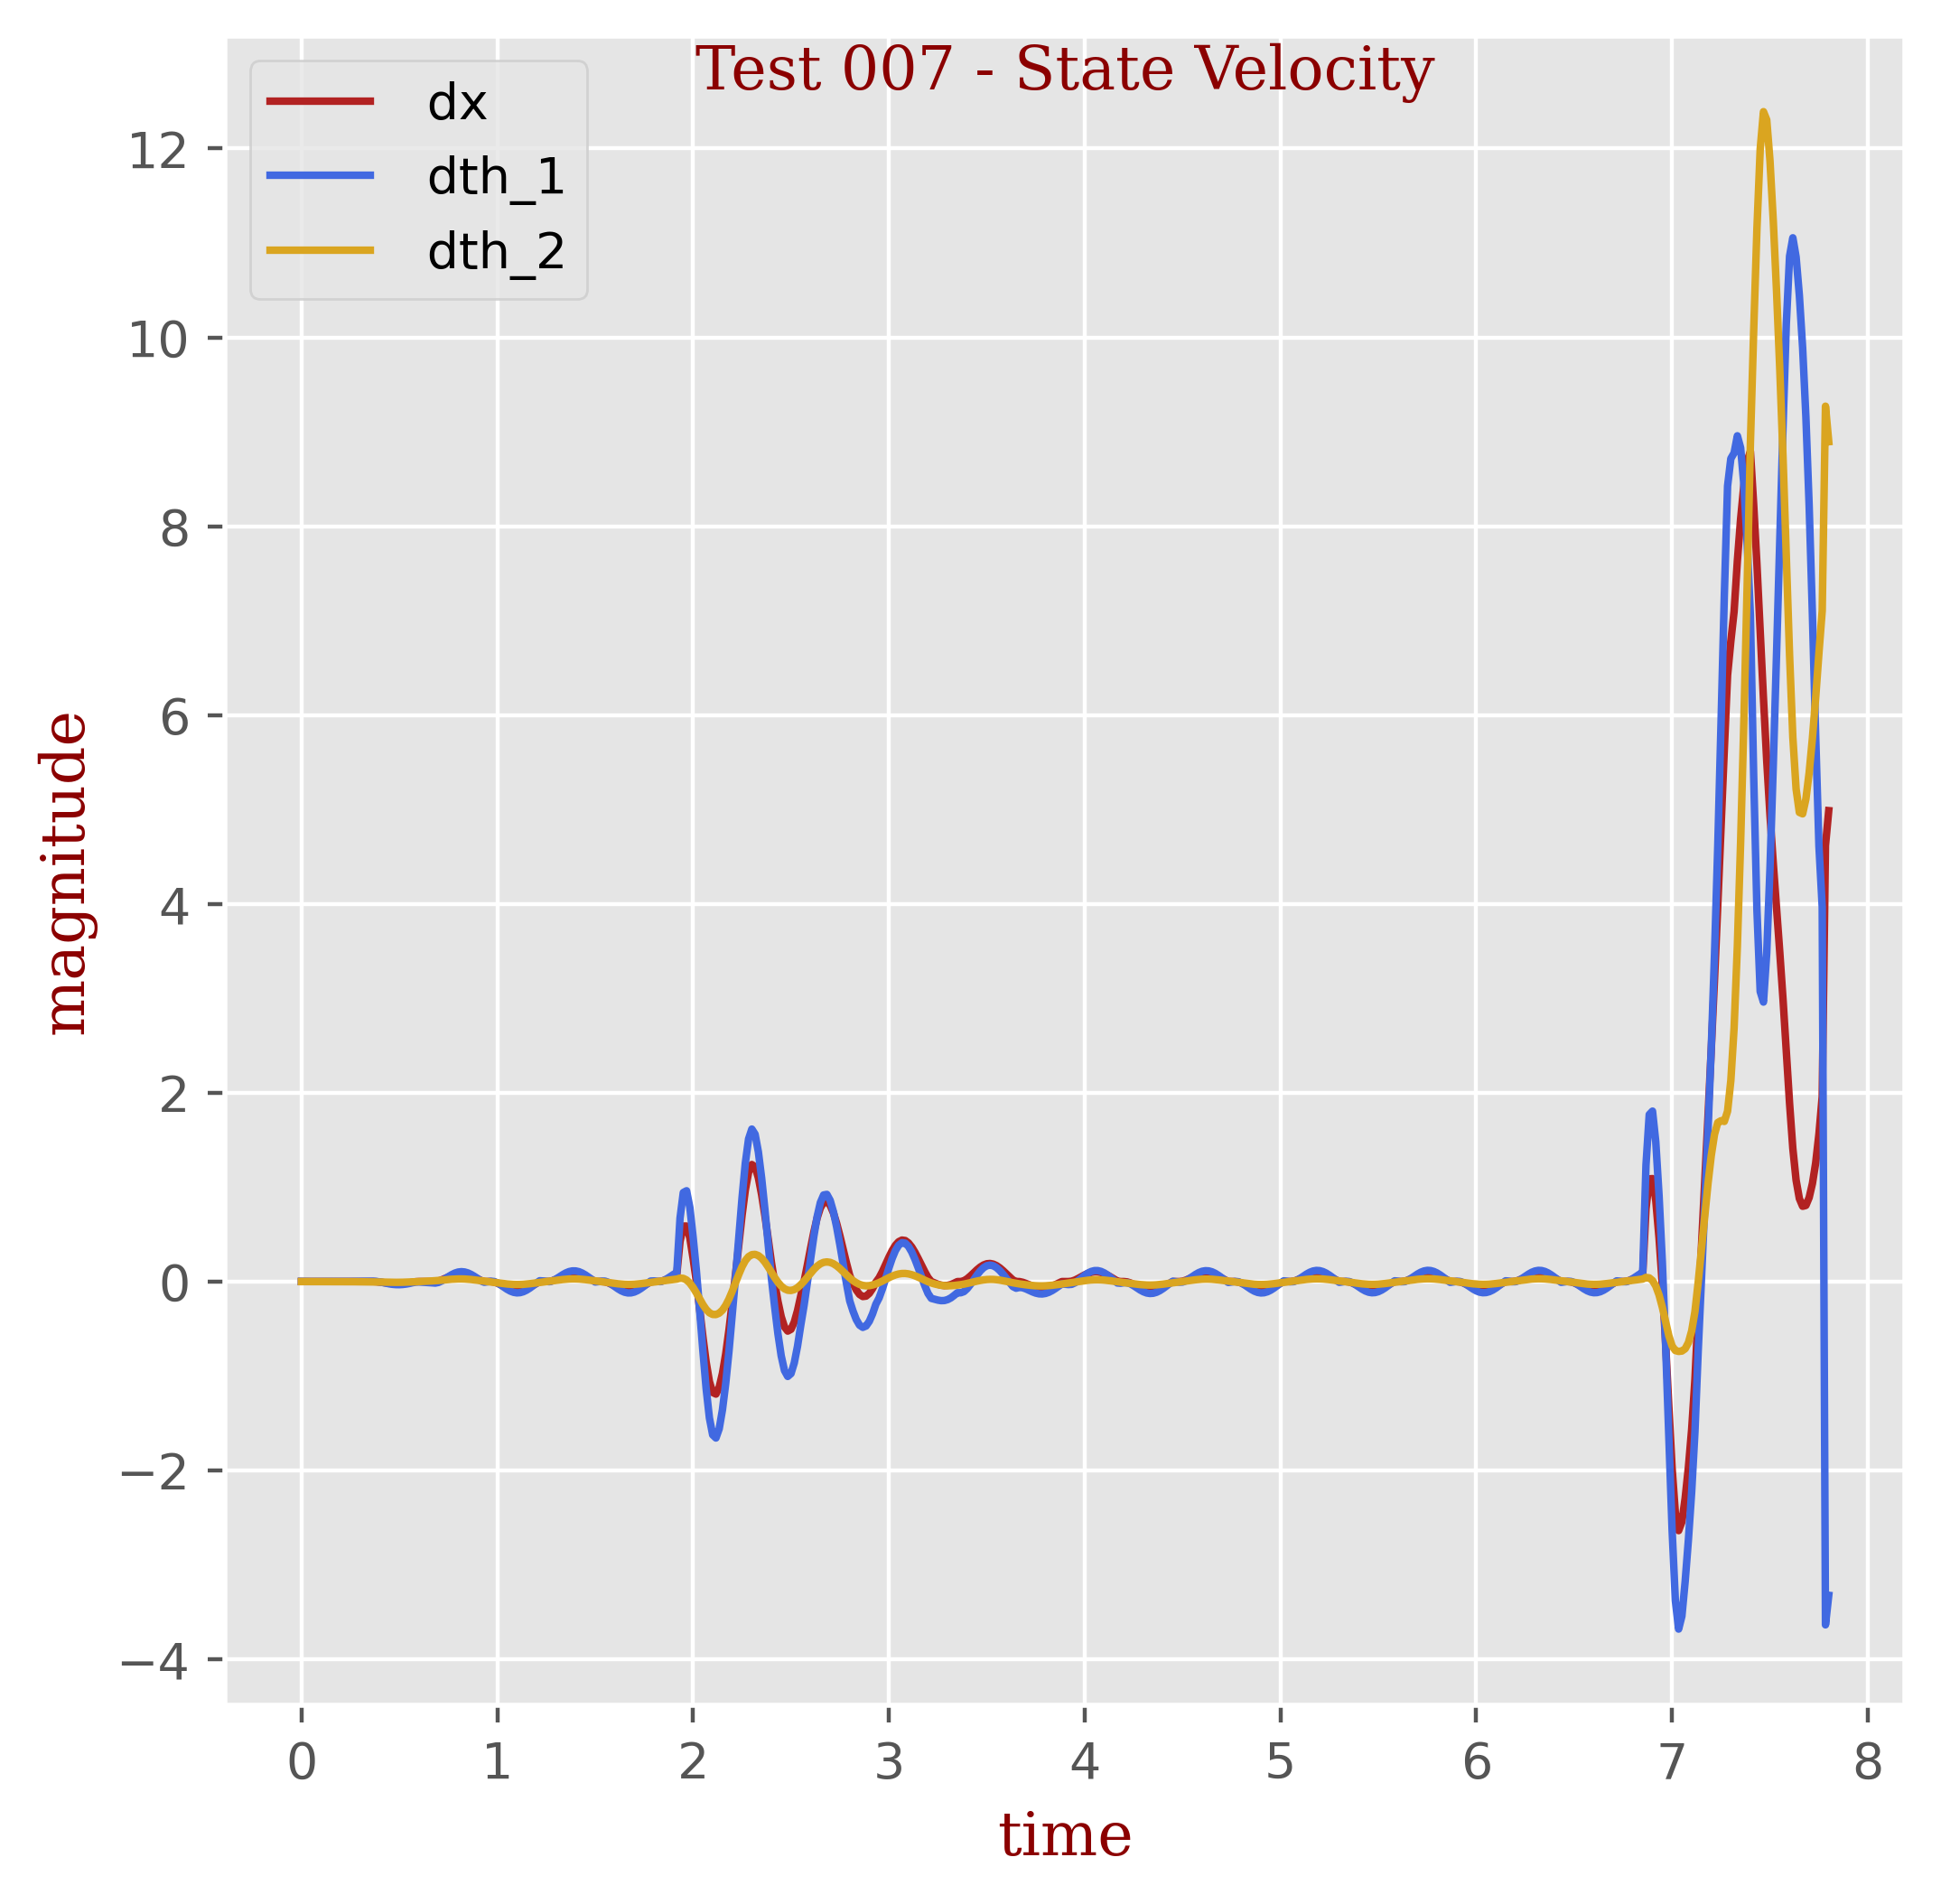
\includegraphics[width=27mm]{Test 007_State_Velocity.png}}
      \subfigure[\(J(t)\)]{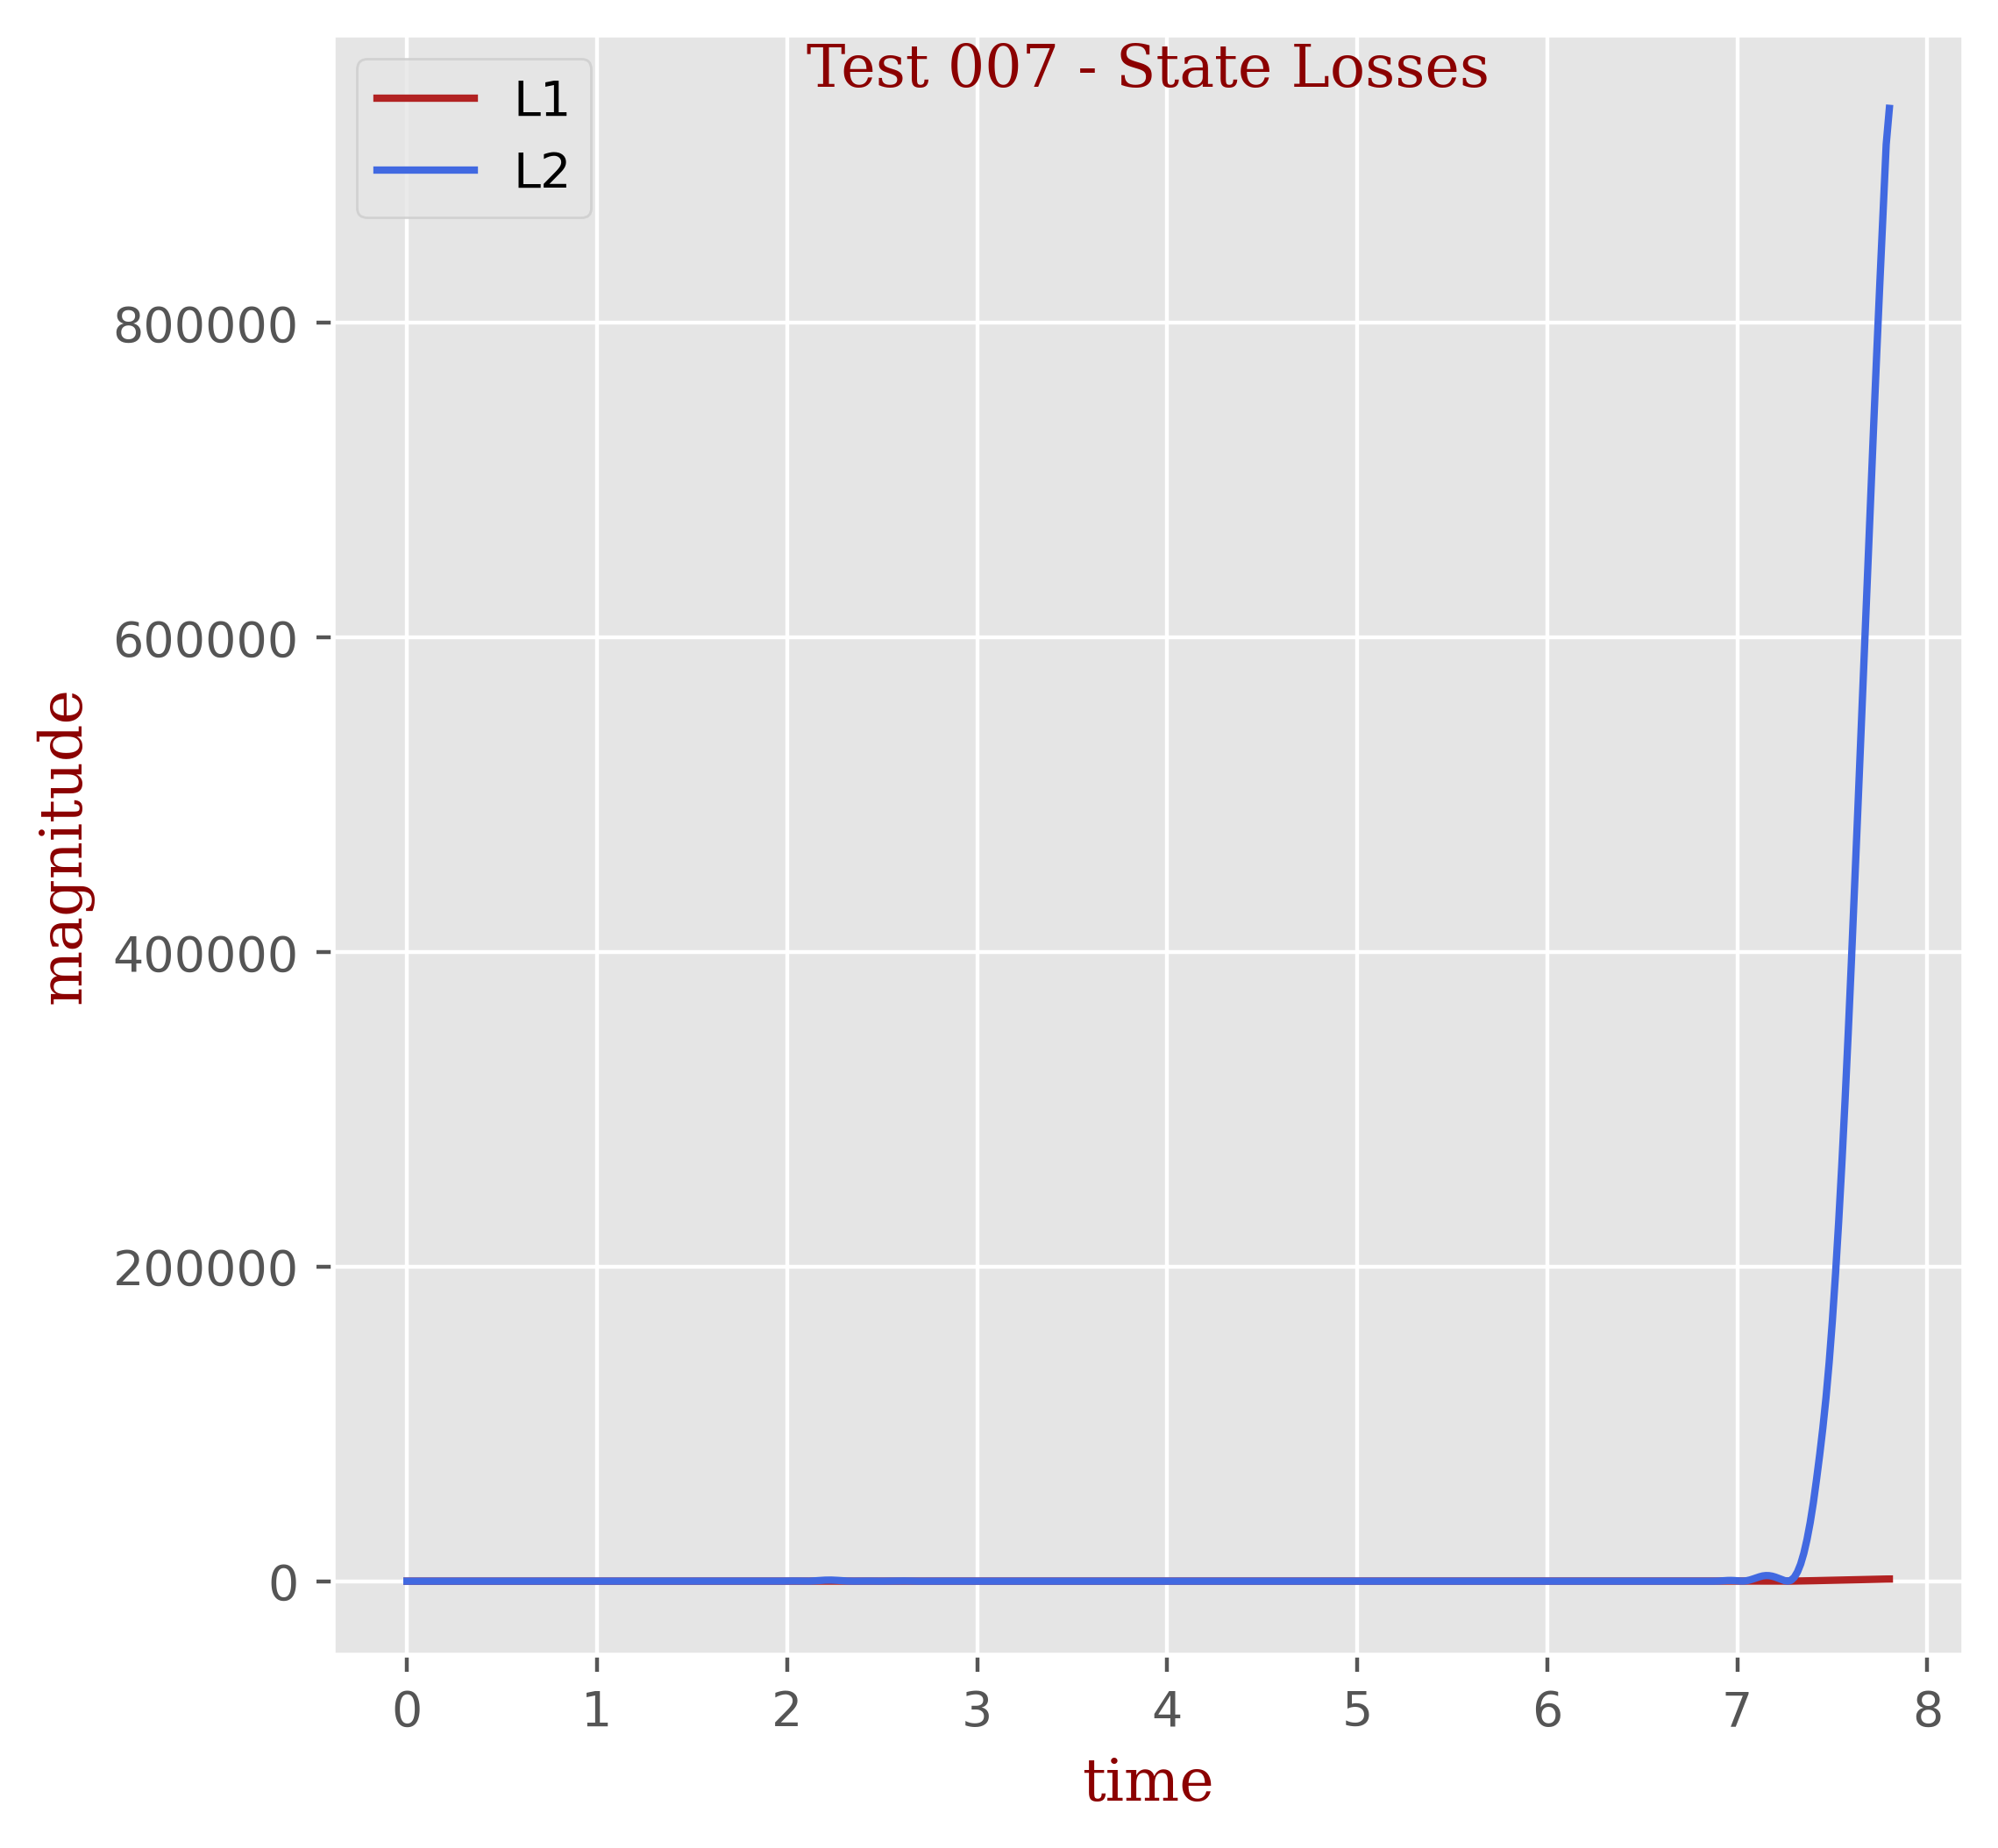
\includegraphics[width=27mm]{Test 007_State_Losses.png}}
\caption{Test 005}
\label{fig:t005}
\end{figure}


\begin{figure}
\centering
      \subfigure[\(q(t)\)]{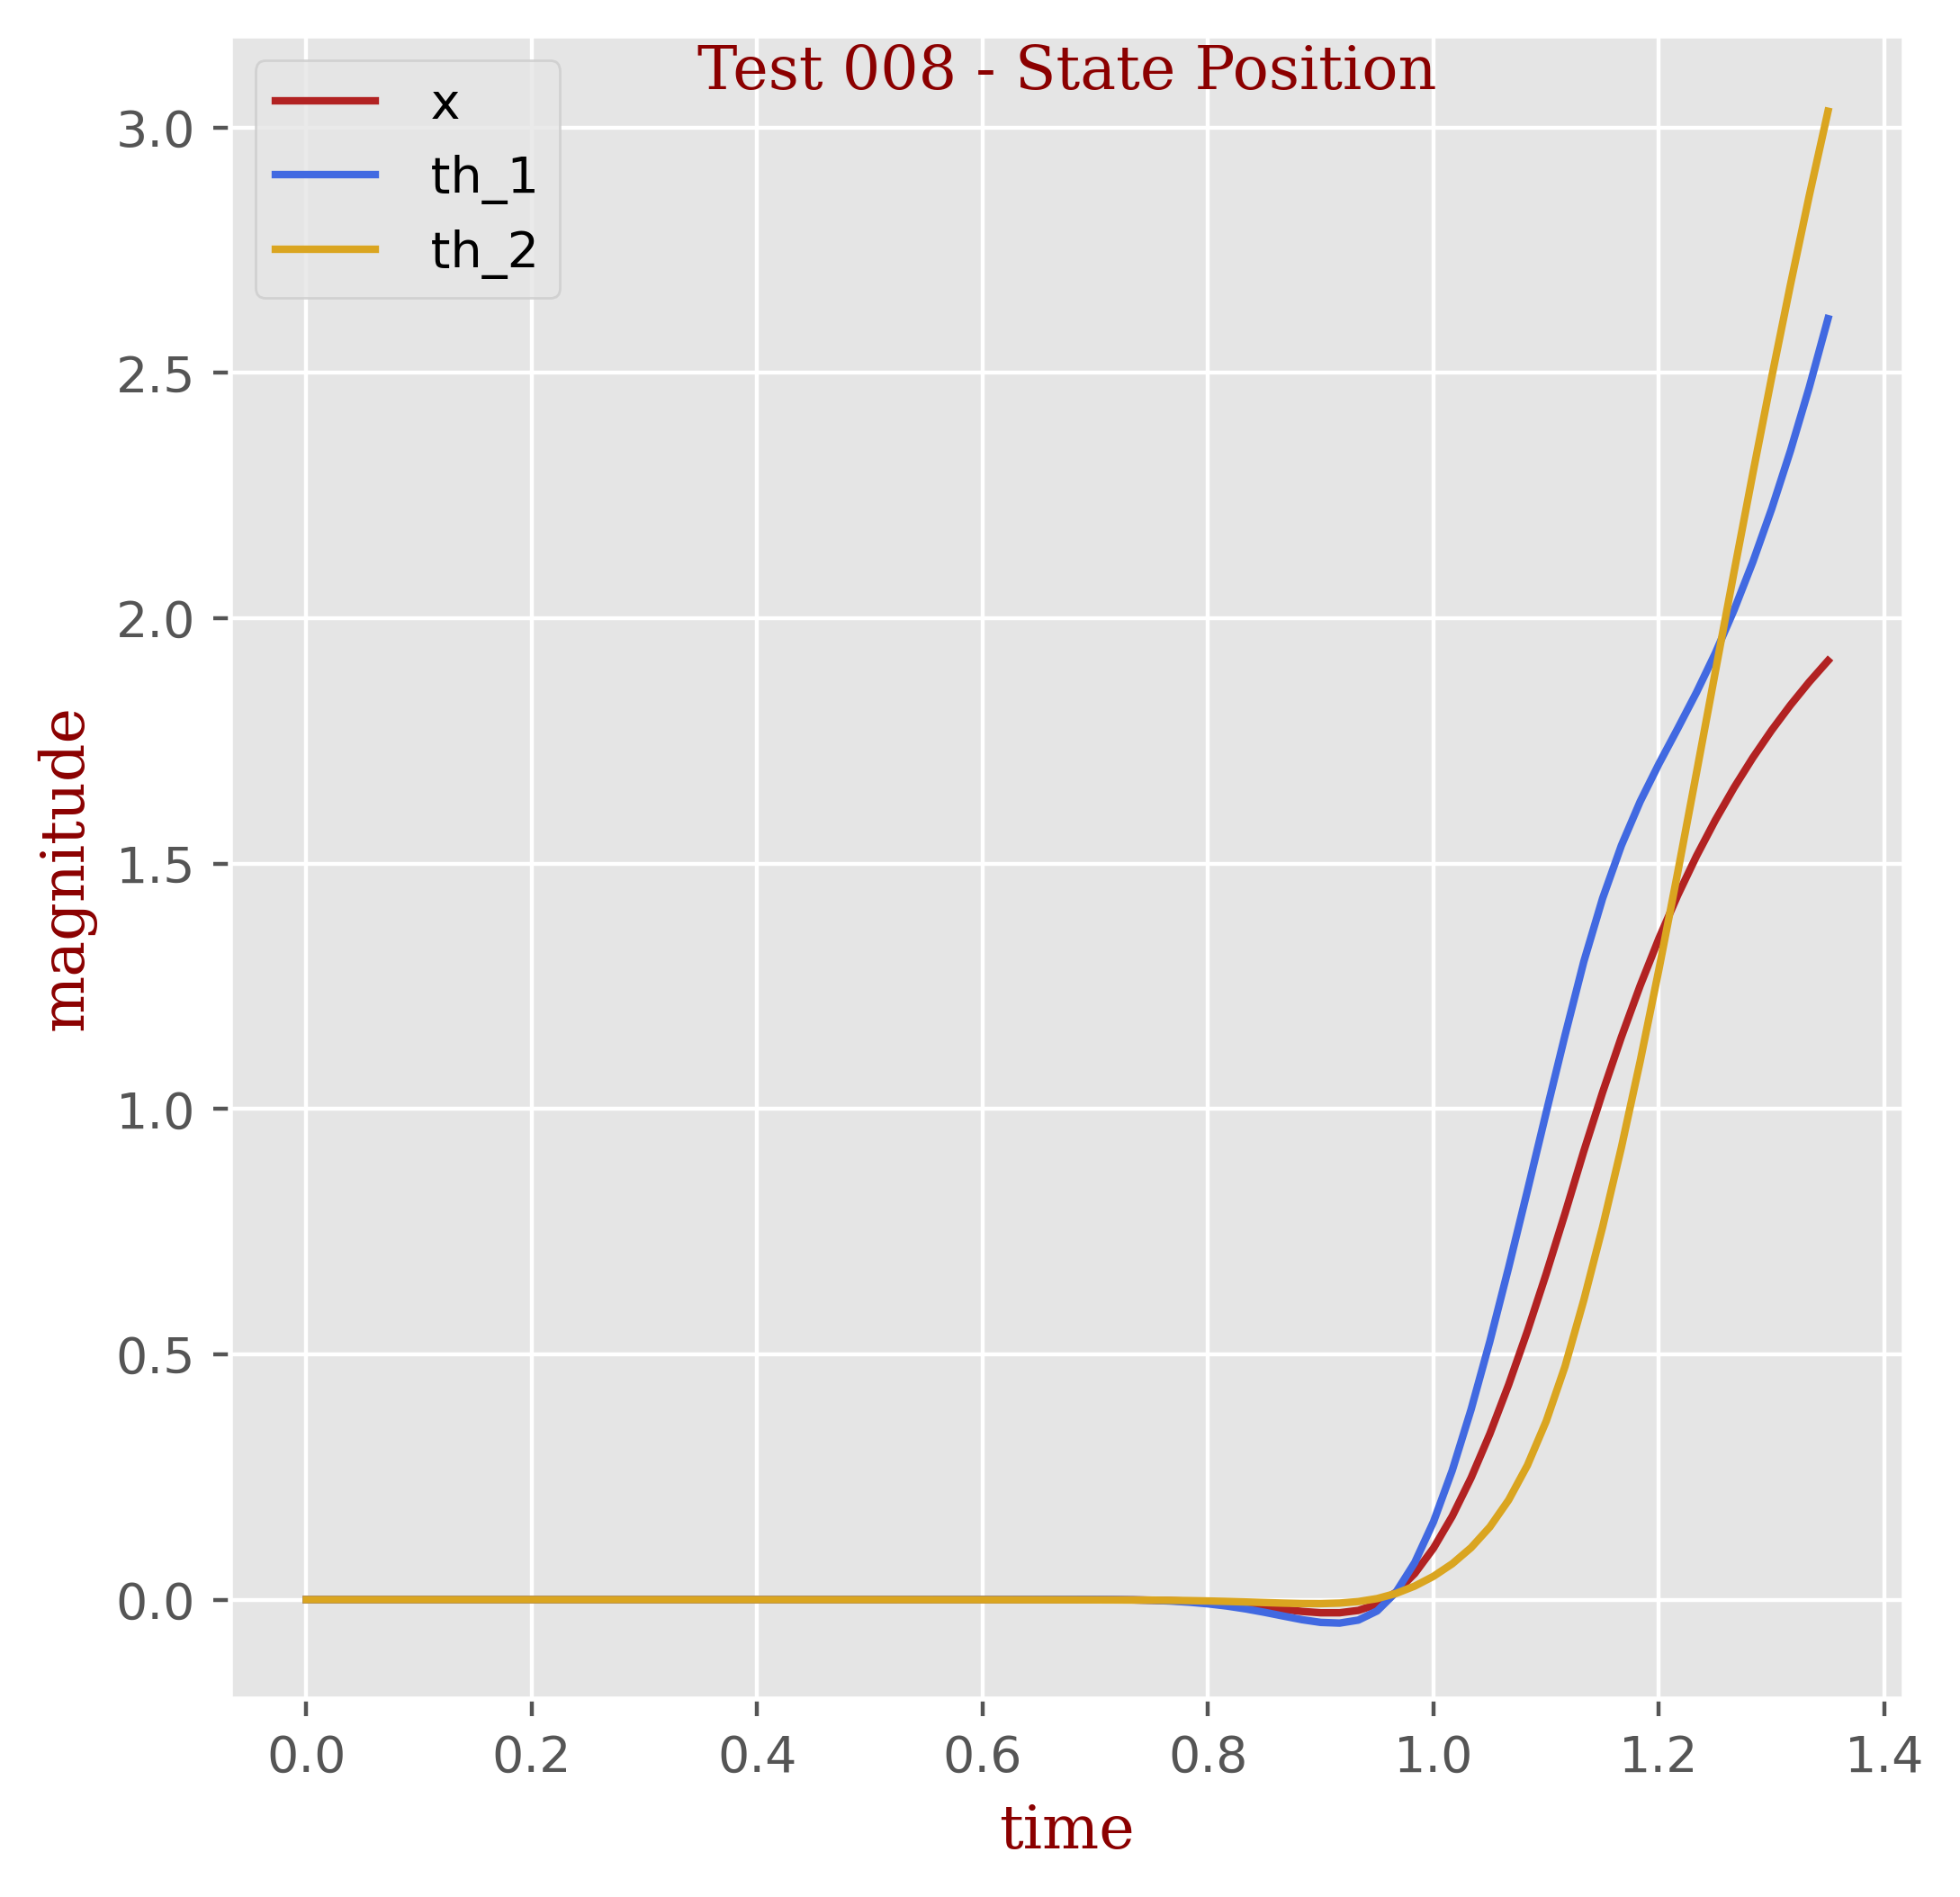
\includegraphics[width=27mm]{Test 008_State_Position.png}}
\subfigure[\(\dot{q}(t)\)]{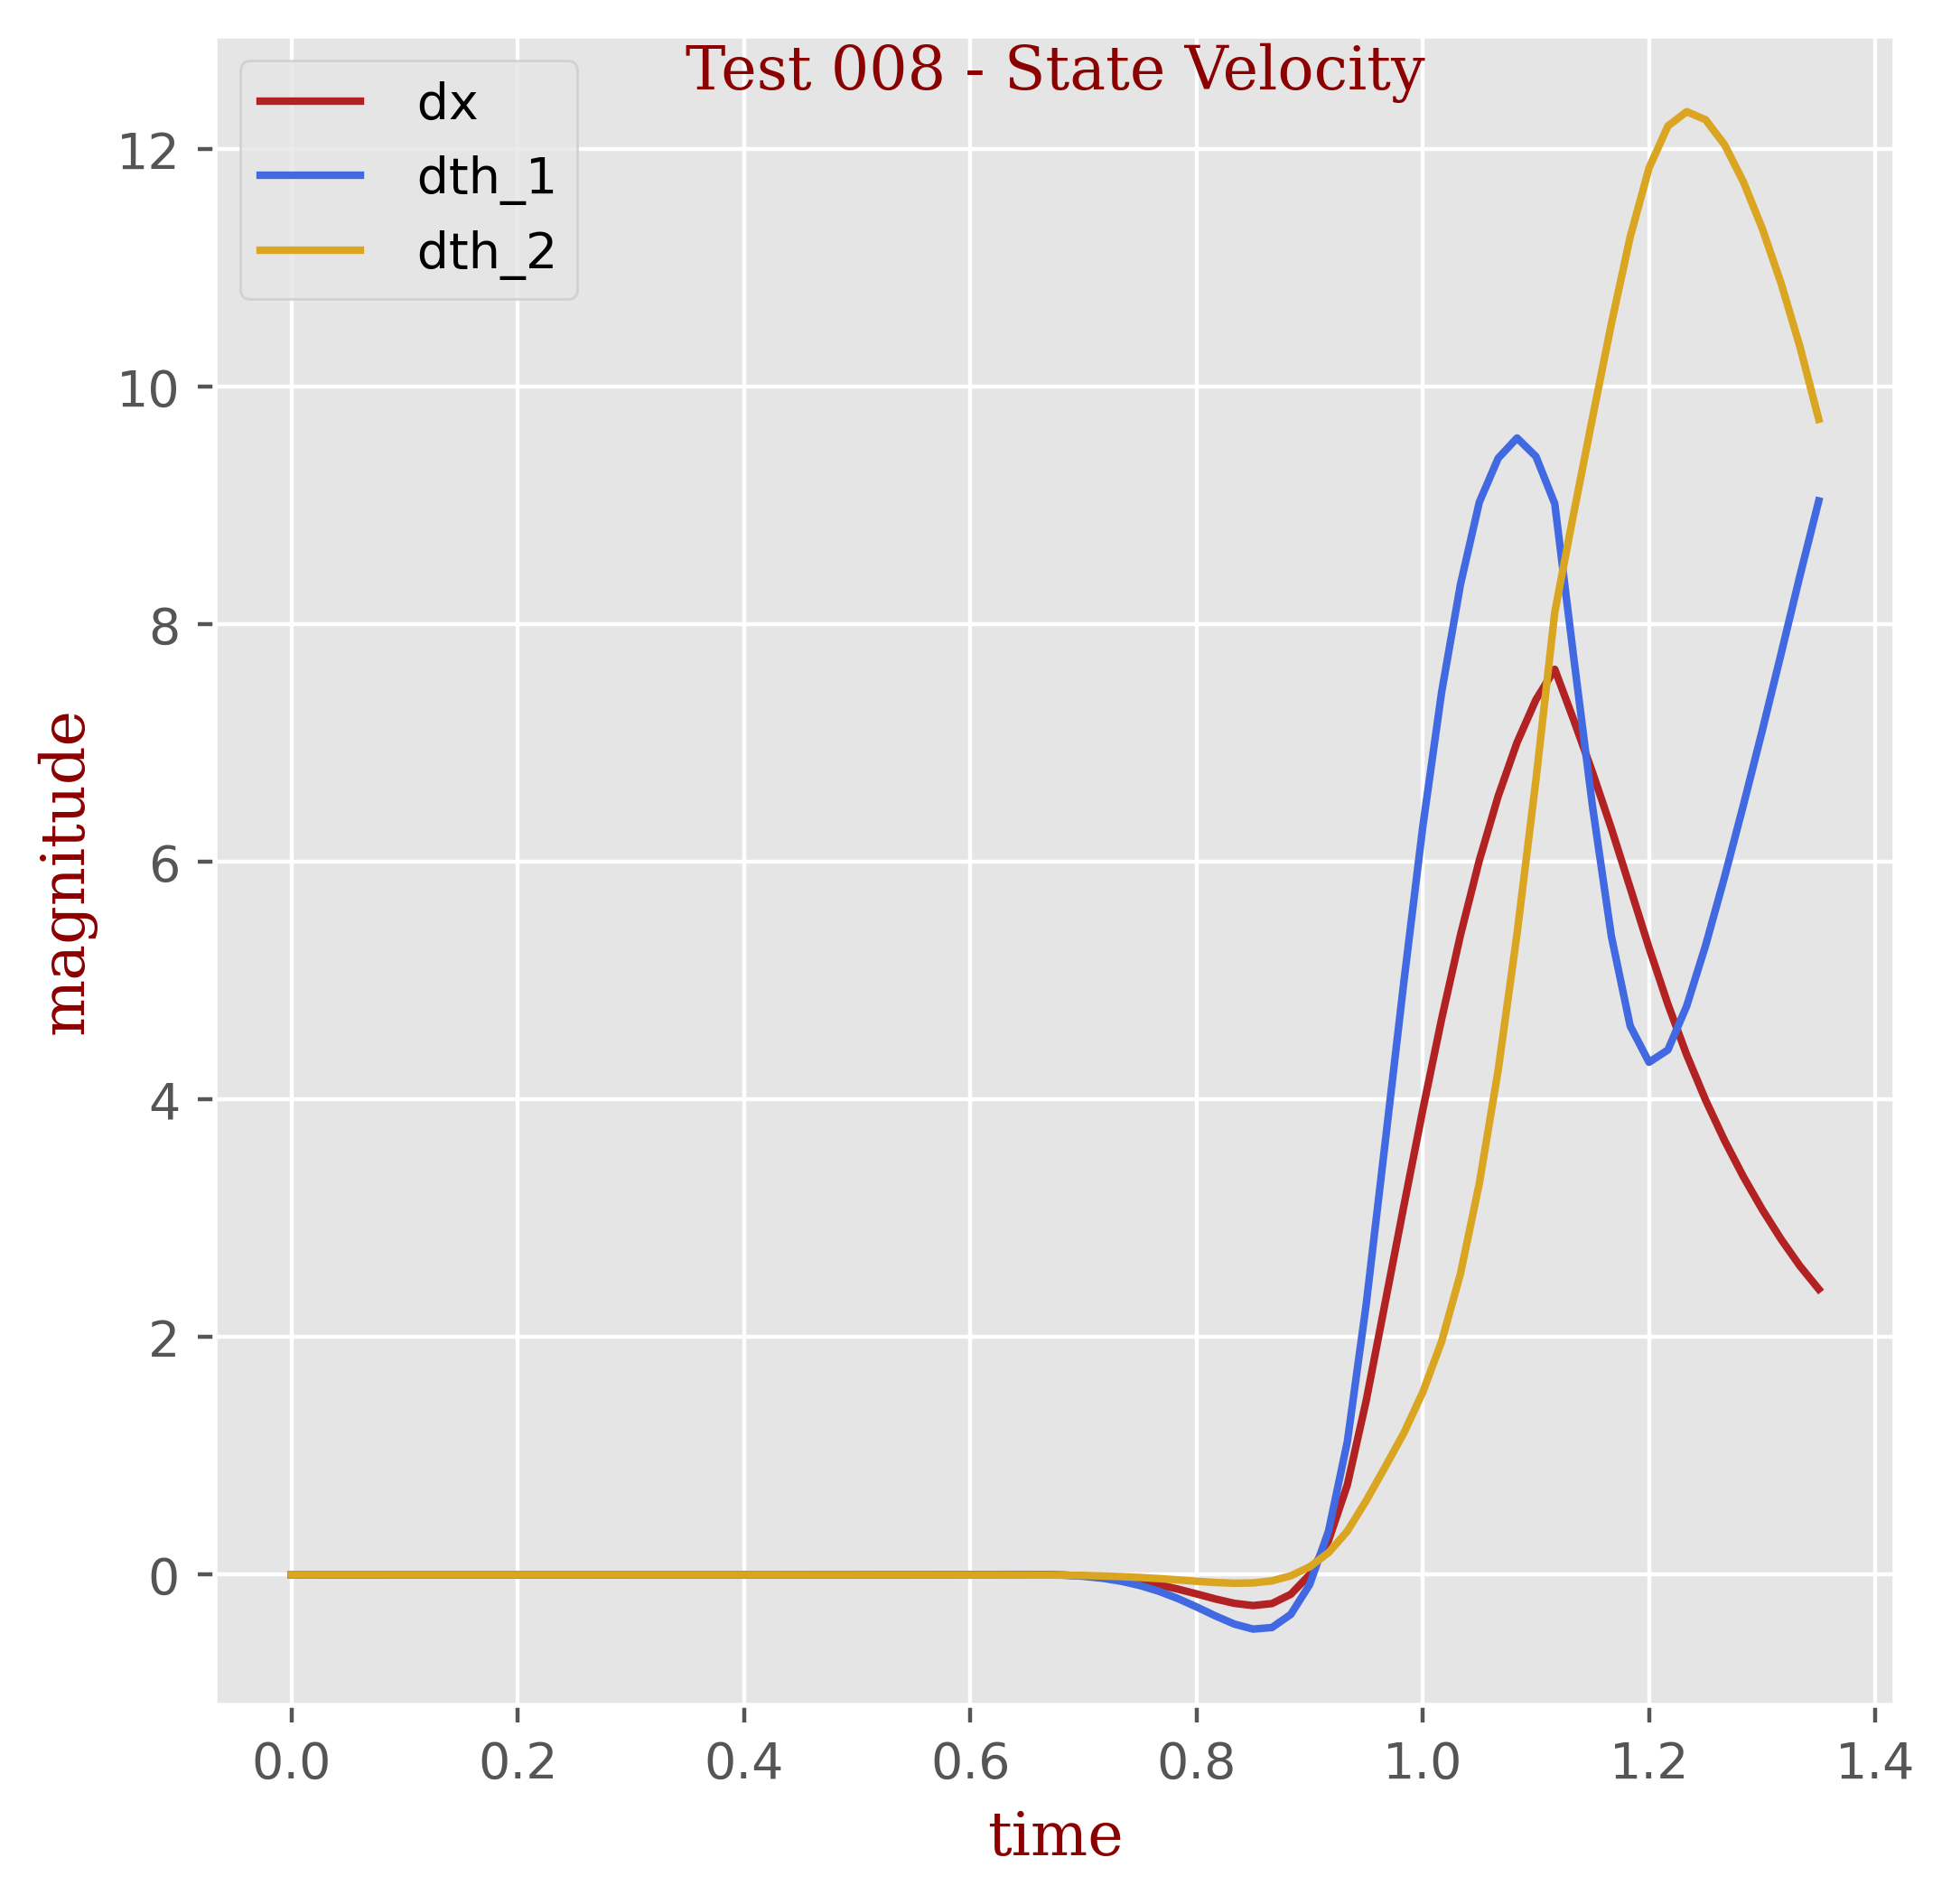
\includegraphics[width=27mm]{Test 008_State_Velocity.png}}
      \subfigure[\(J(t)\)]{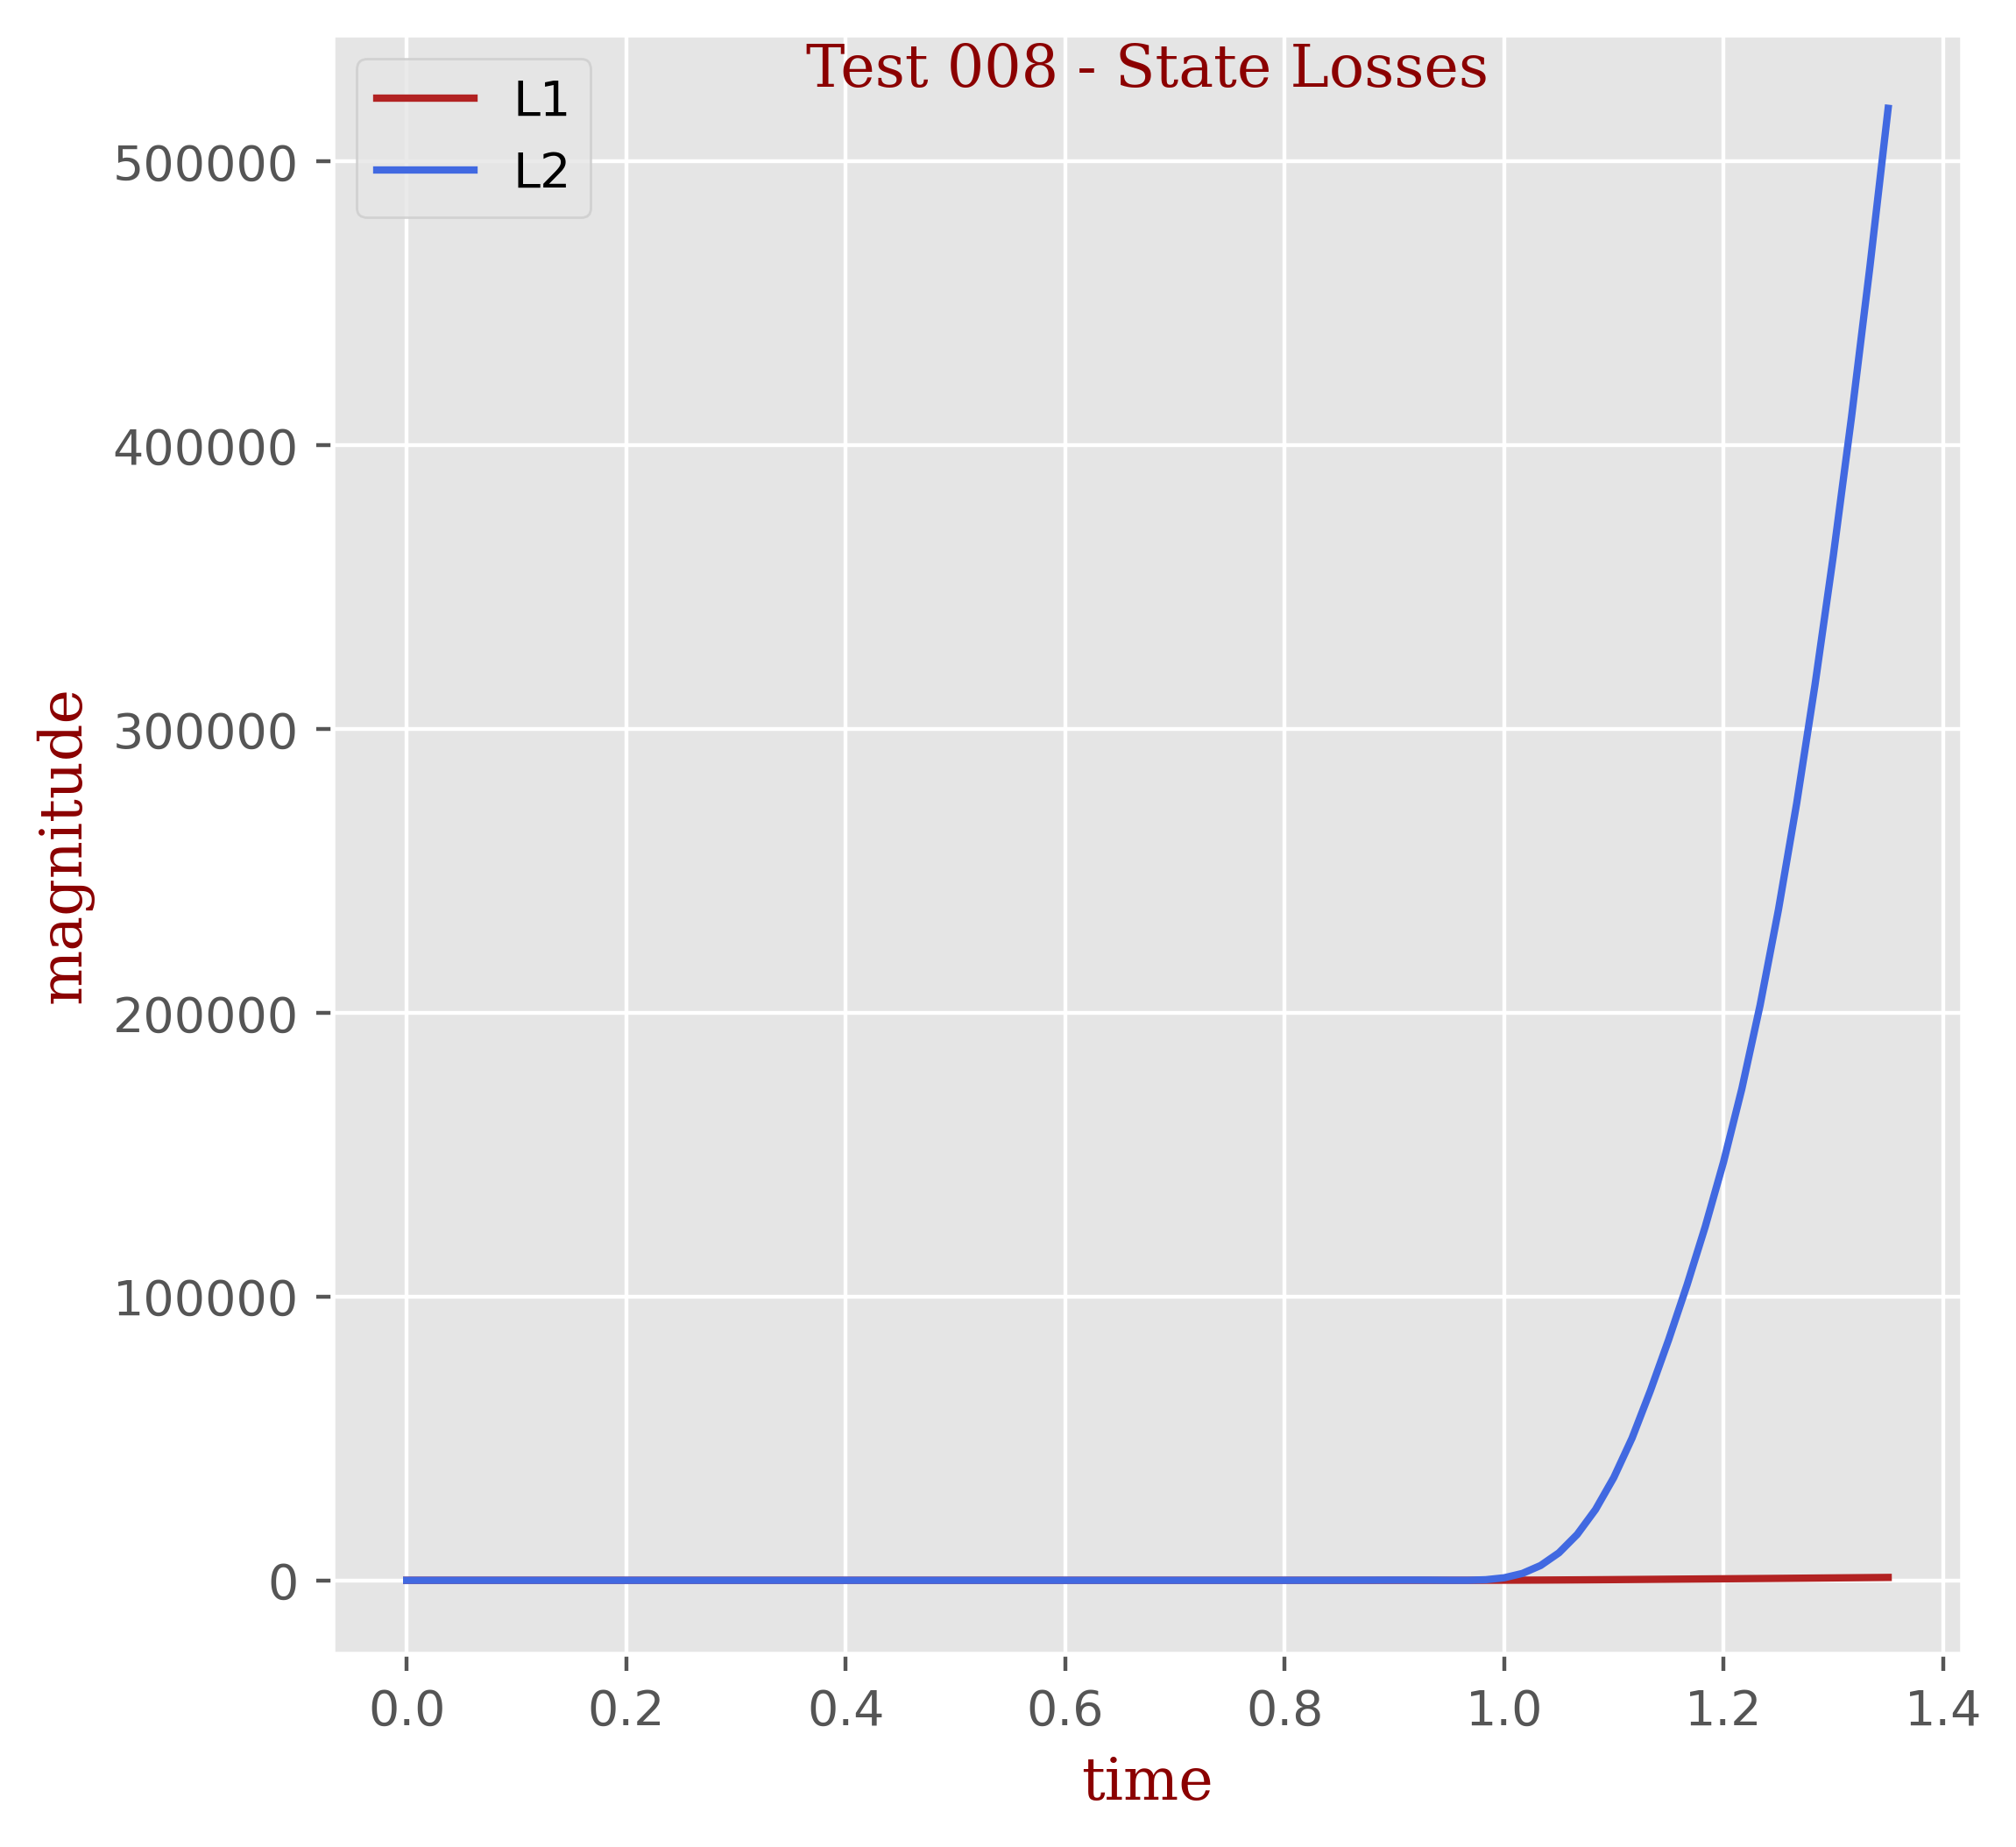
\includegraphics[width=27mm]{Test 008_State_Losses.png}}
                                               \caption{Test 008}
                                                 \label{fig:t008}
\end{figure}


\begin{figure}
\centering
       \subfigure[\(q(t)\)]{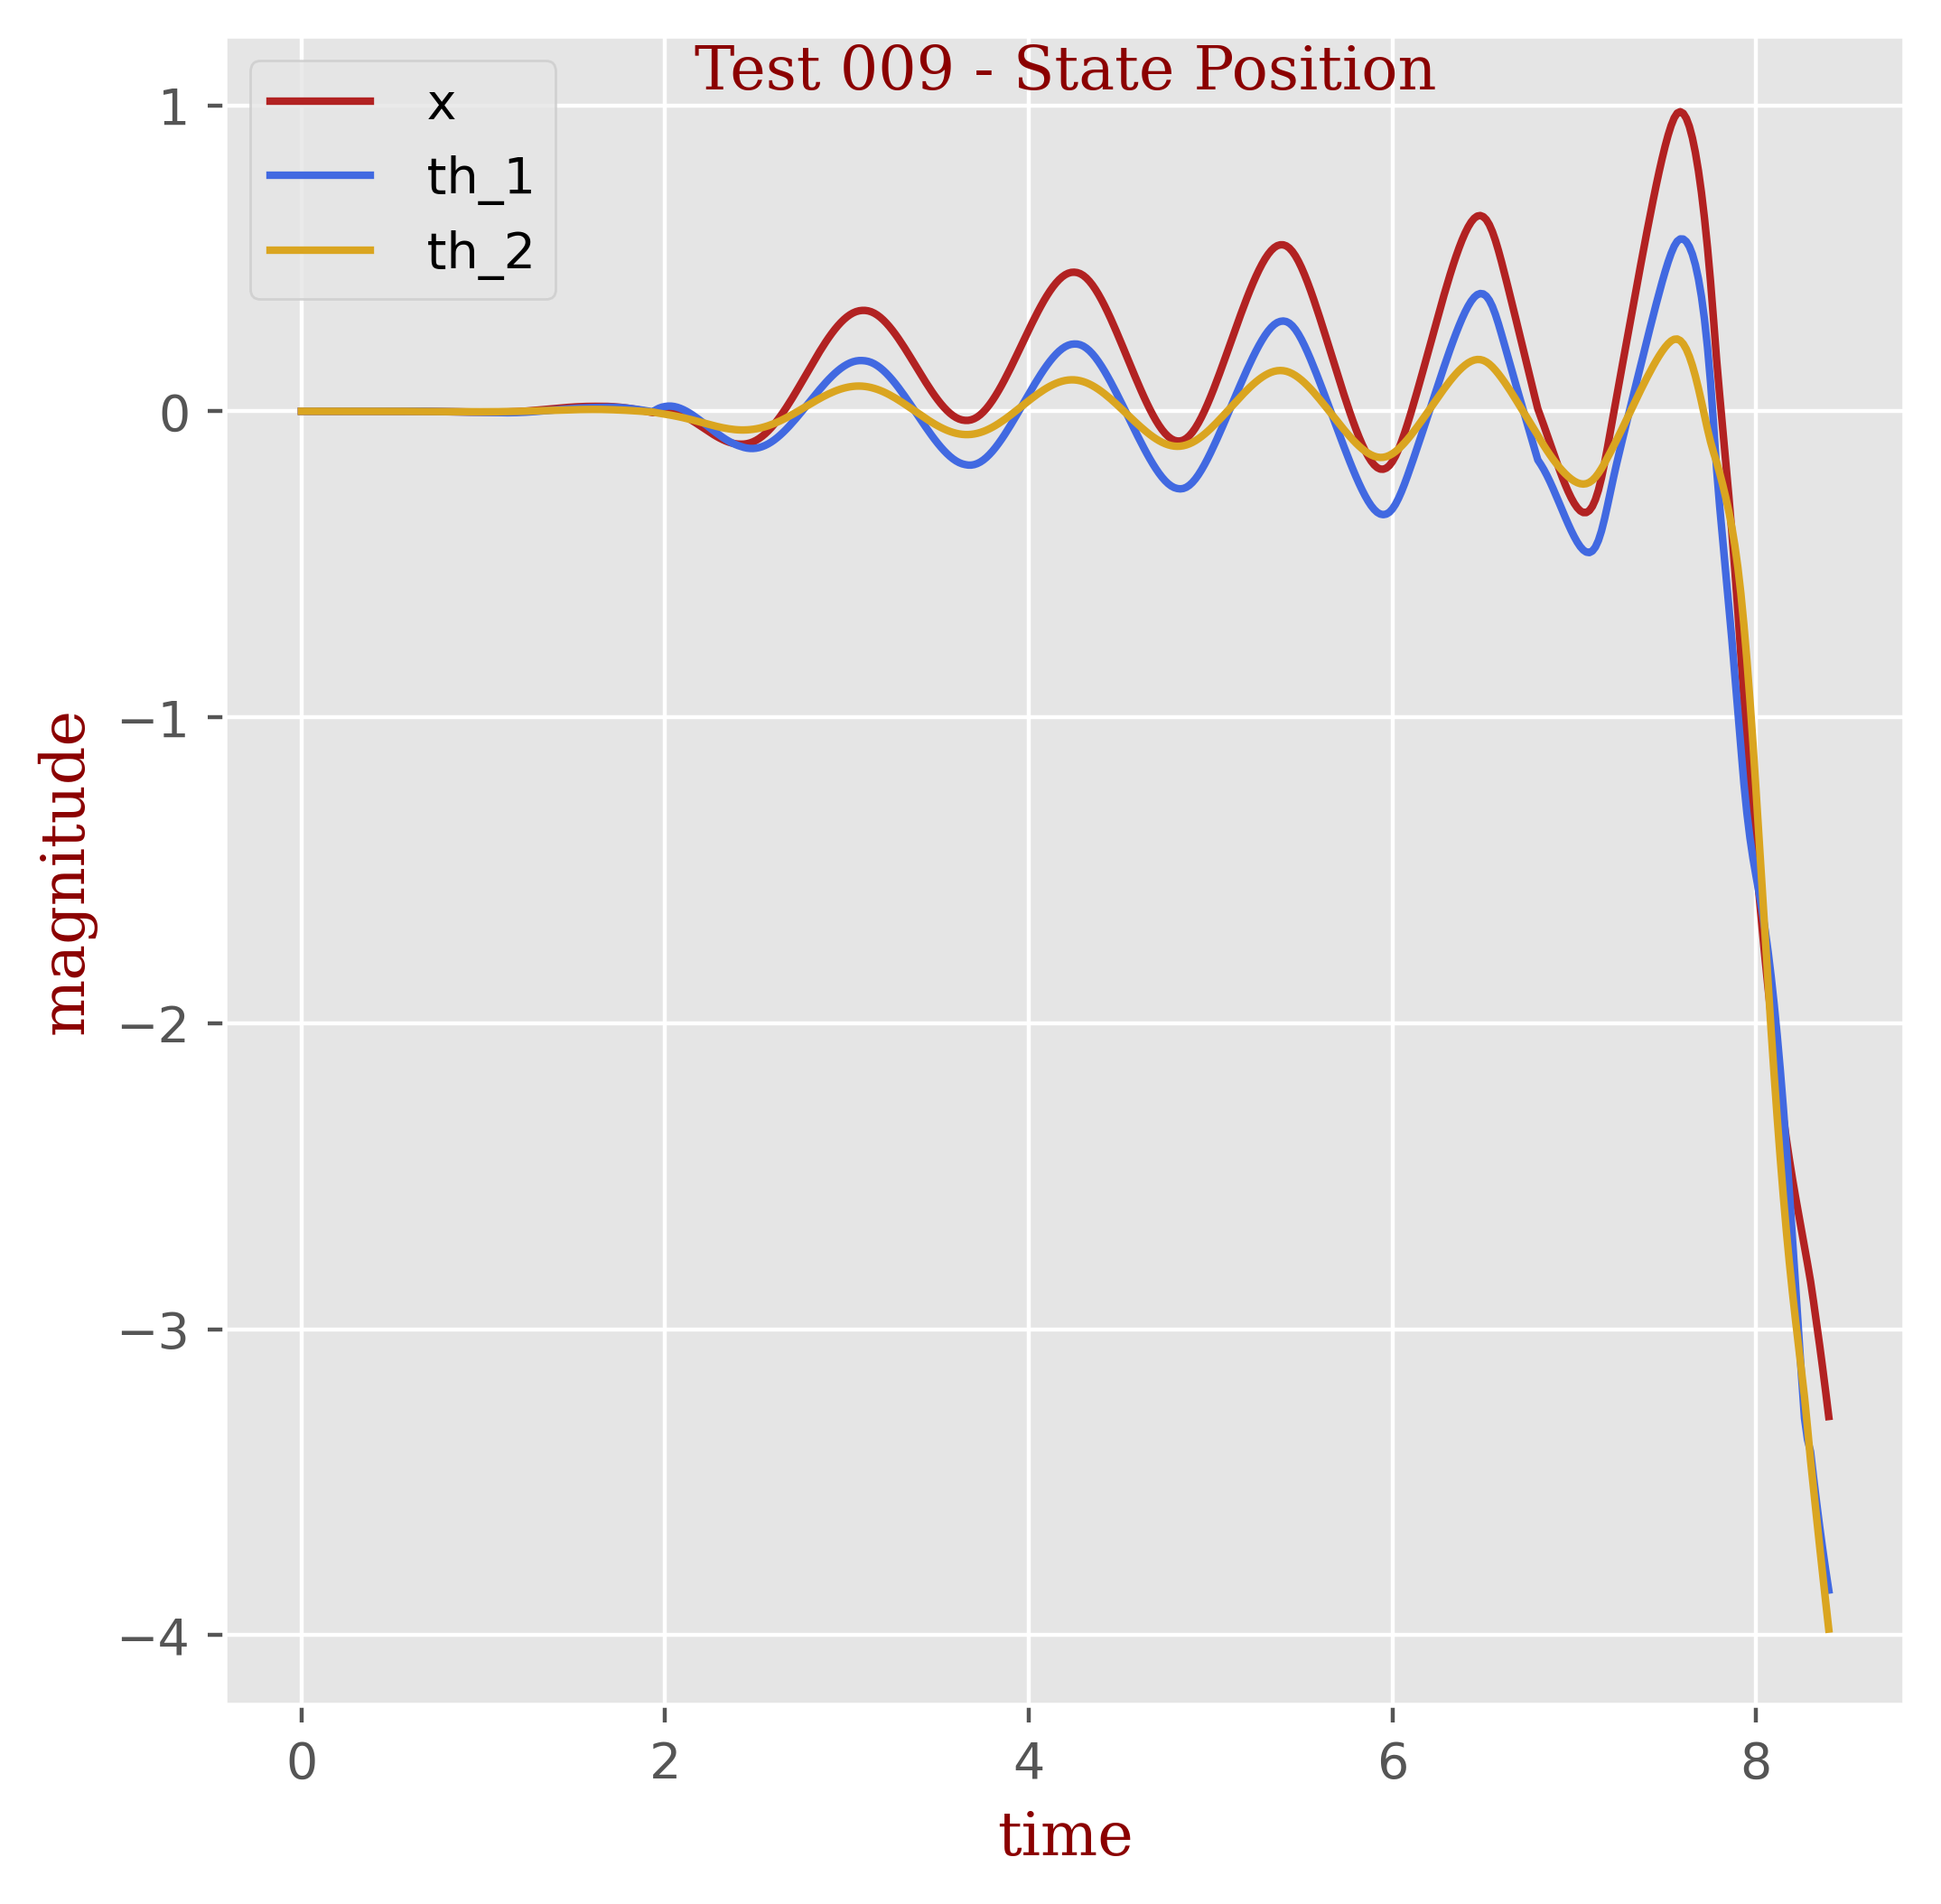
\includegraphics[width=27mm]{Test 009_State_Position.png}}
 \subfigure[\(\dot{q}(t)\)]{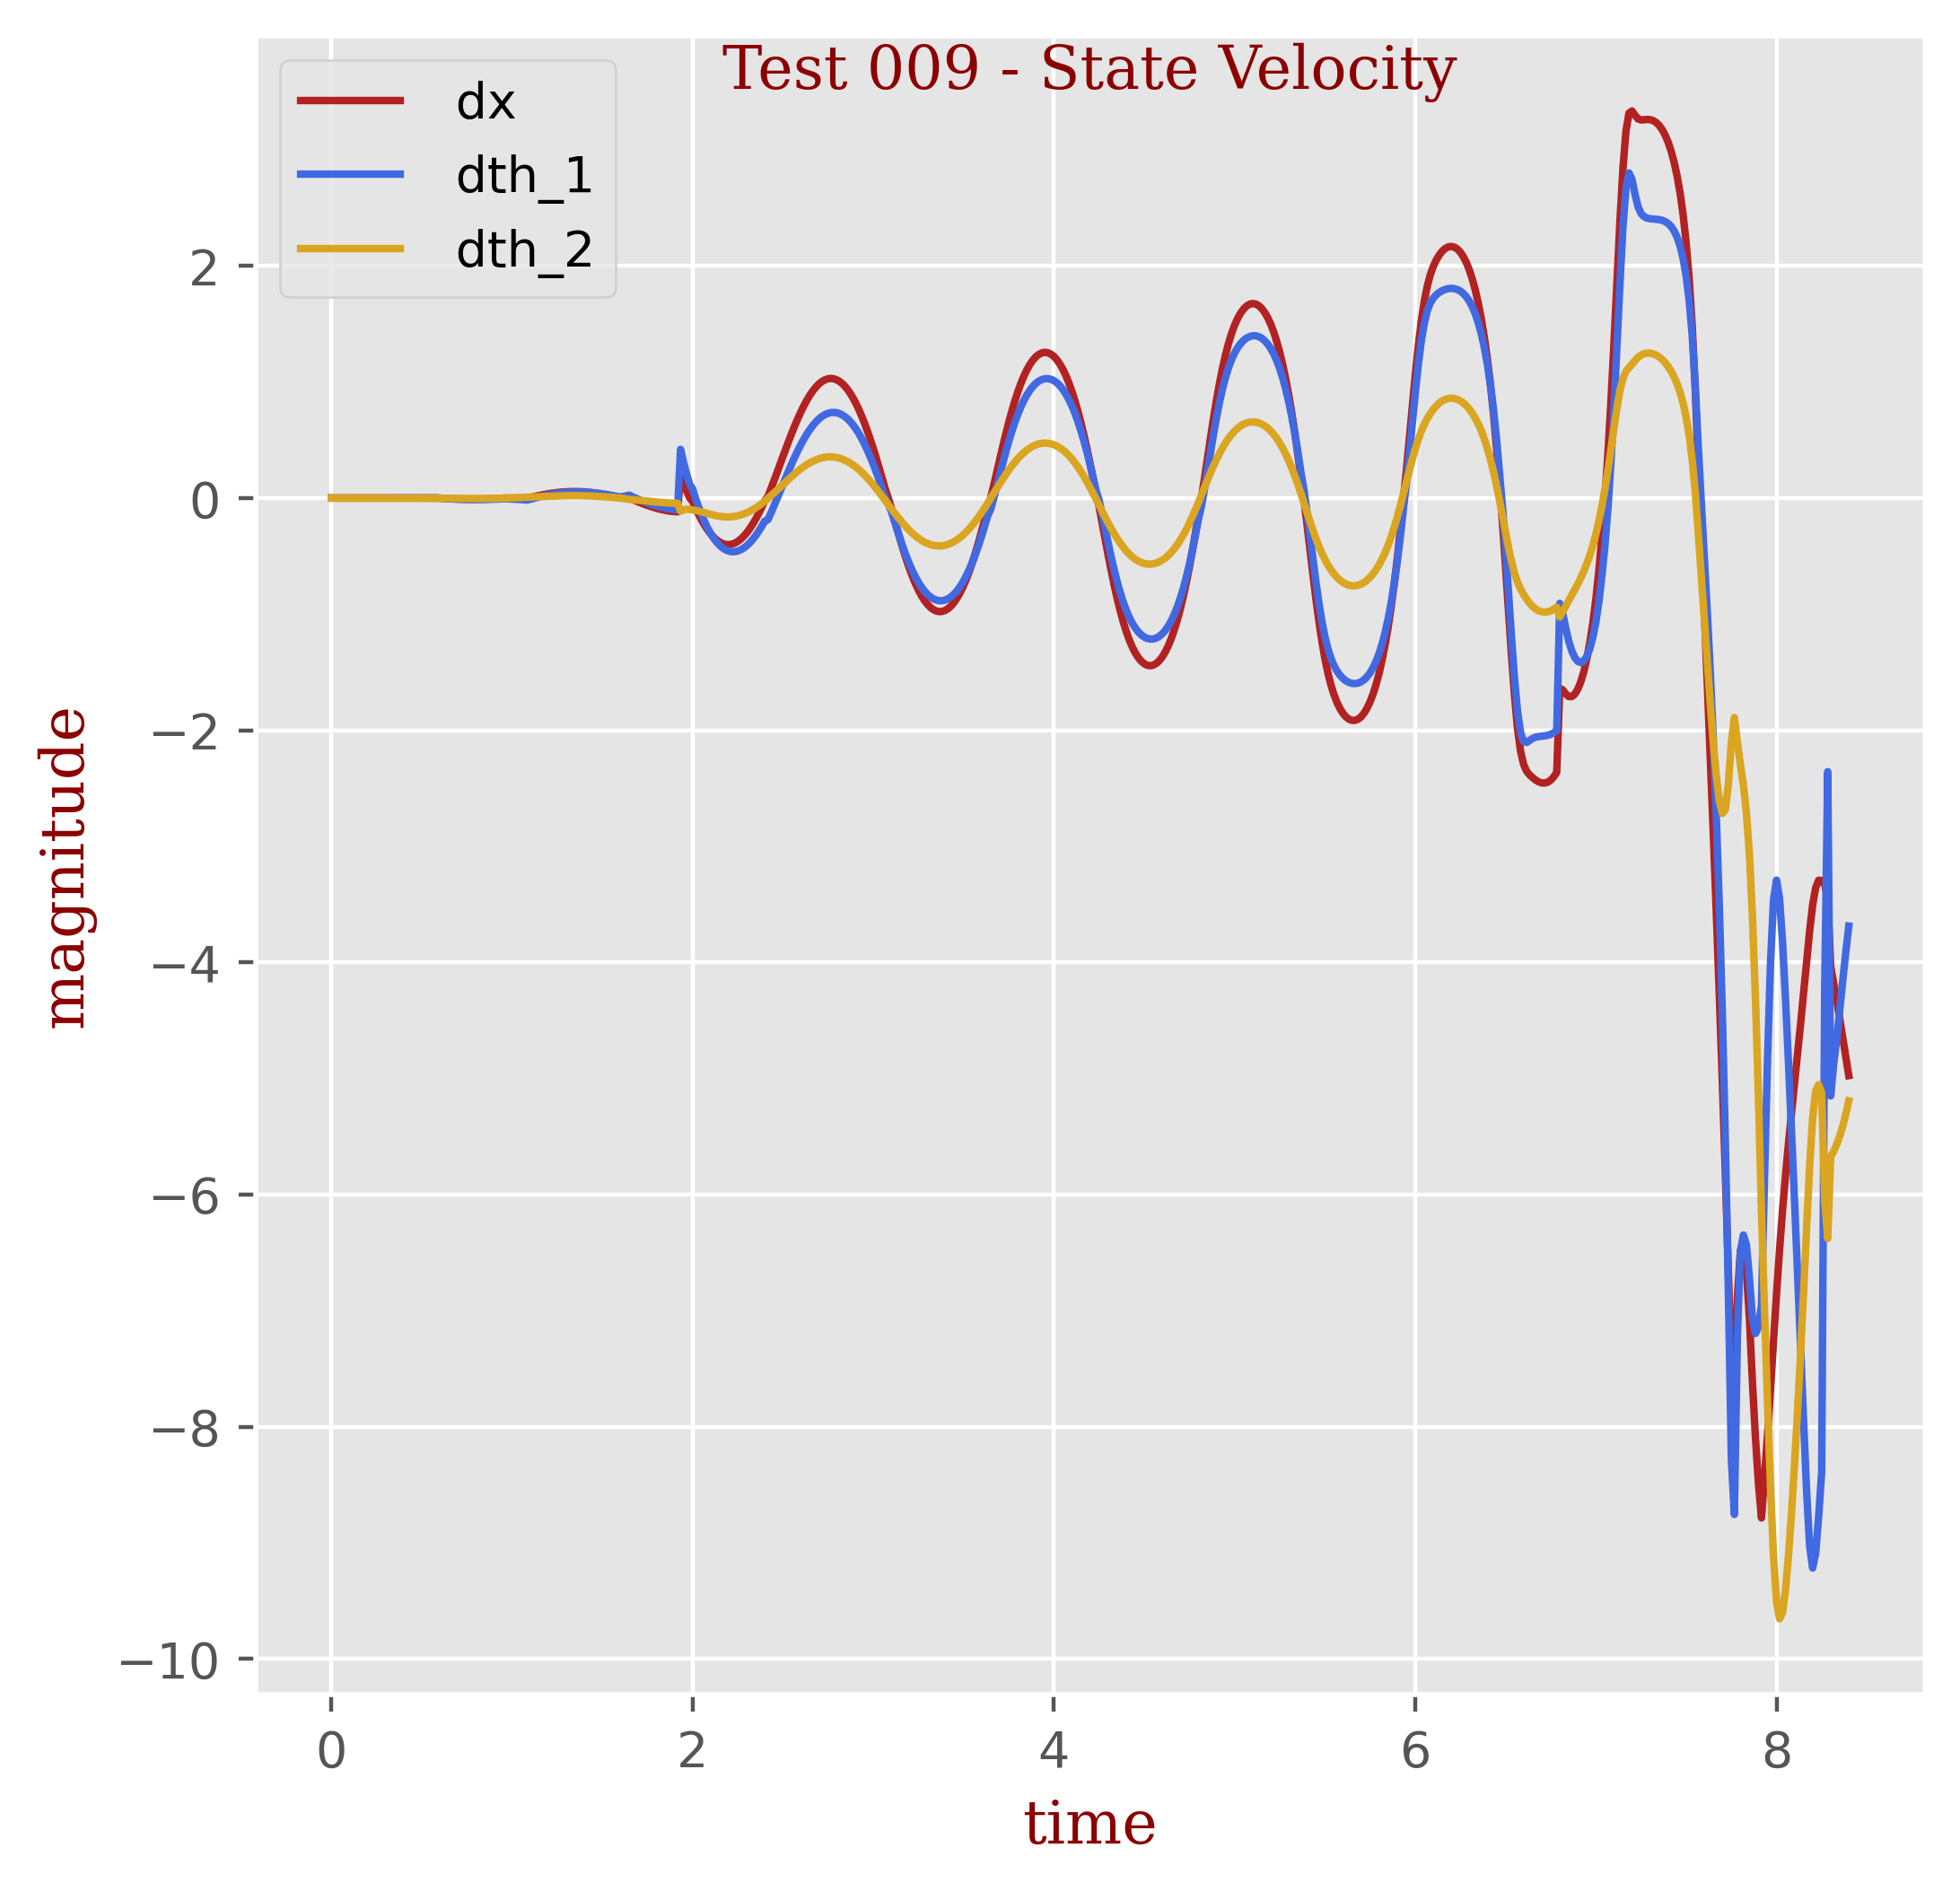
\includegraphics[width=27mm]{Test 009_State_Velocity.png}}
       \subfigure[\(J(t)\)]{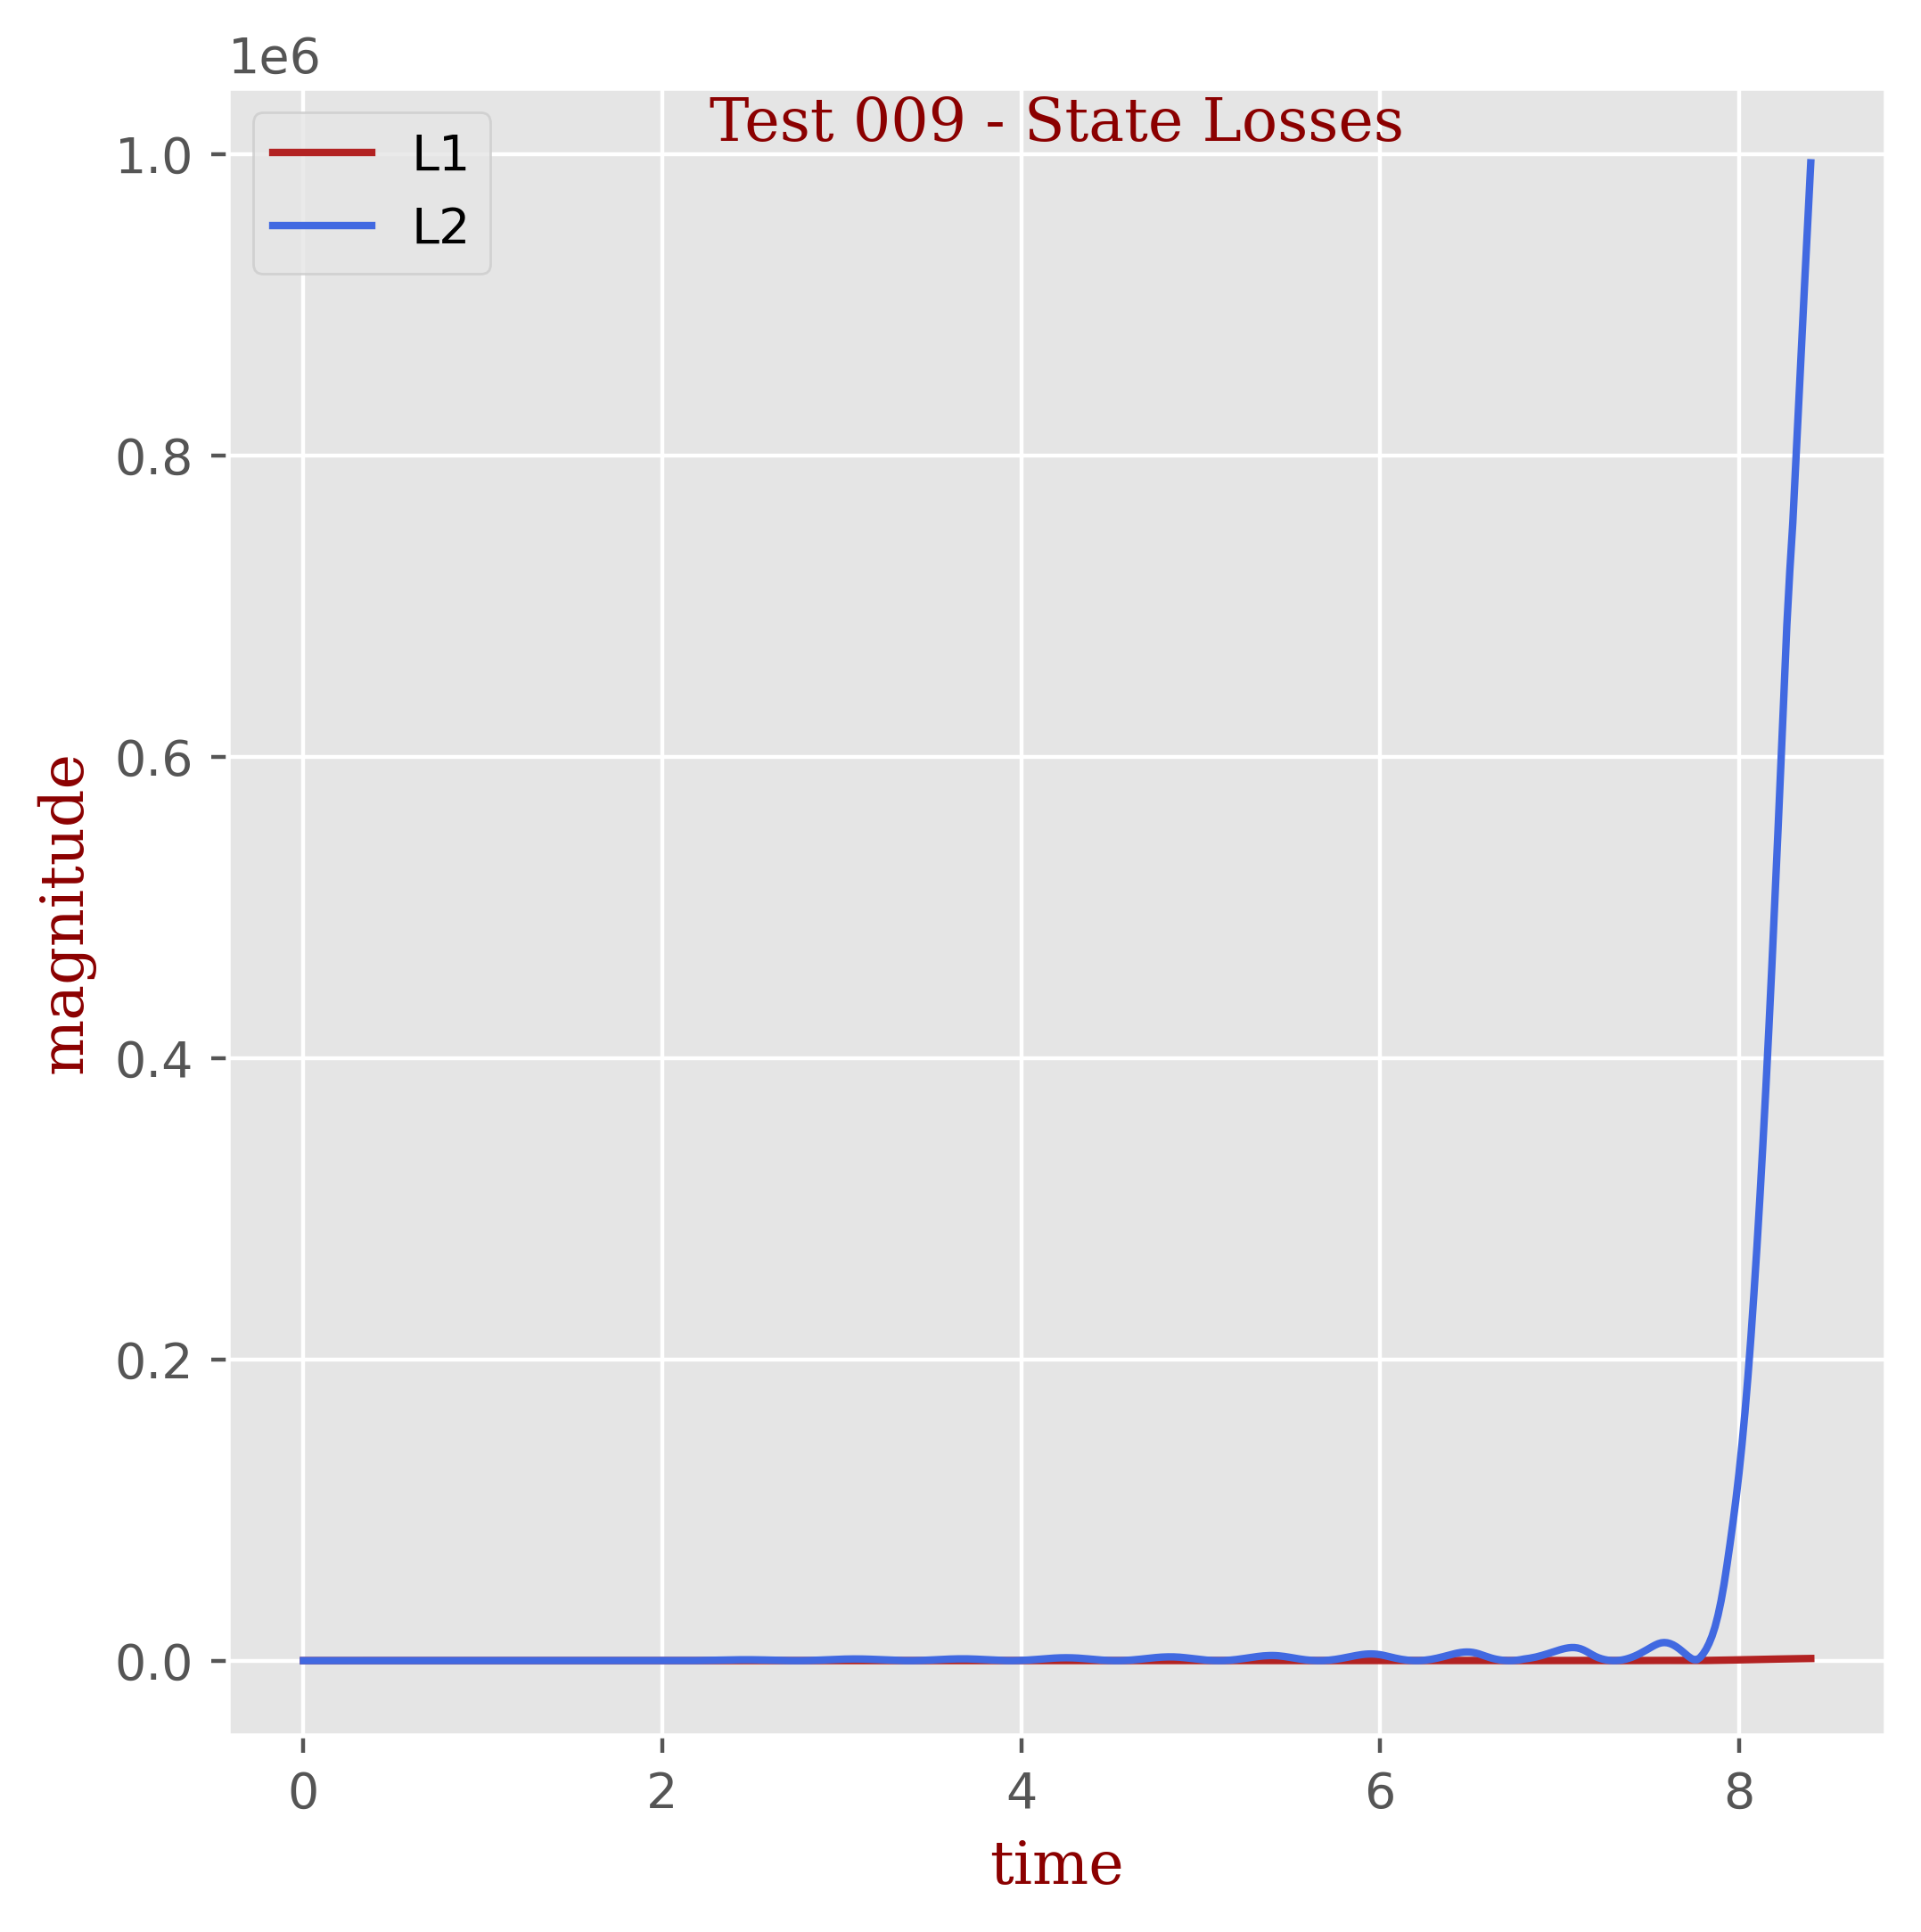
\includegraphics[width=27mm]{Test 009_State_Losses.png}}
                                                \caption{Test 009}
                                                  \label{fig:t009}
\end{figure}


\begin{figure}
    \centering
           \subfigure[\(q(t)\)]{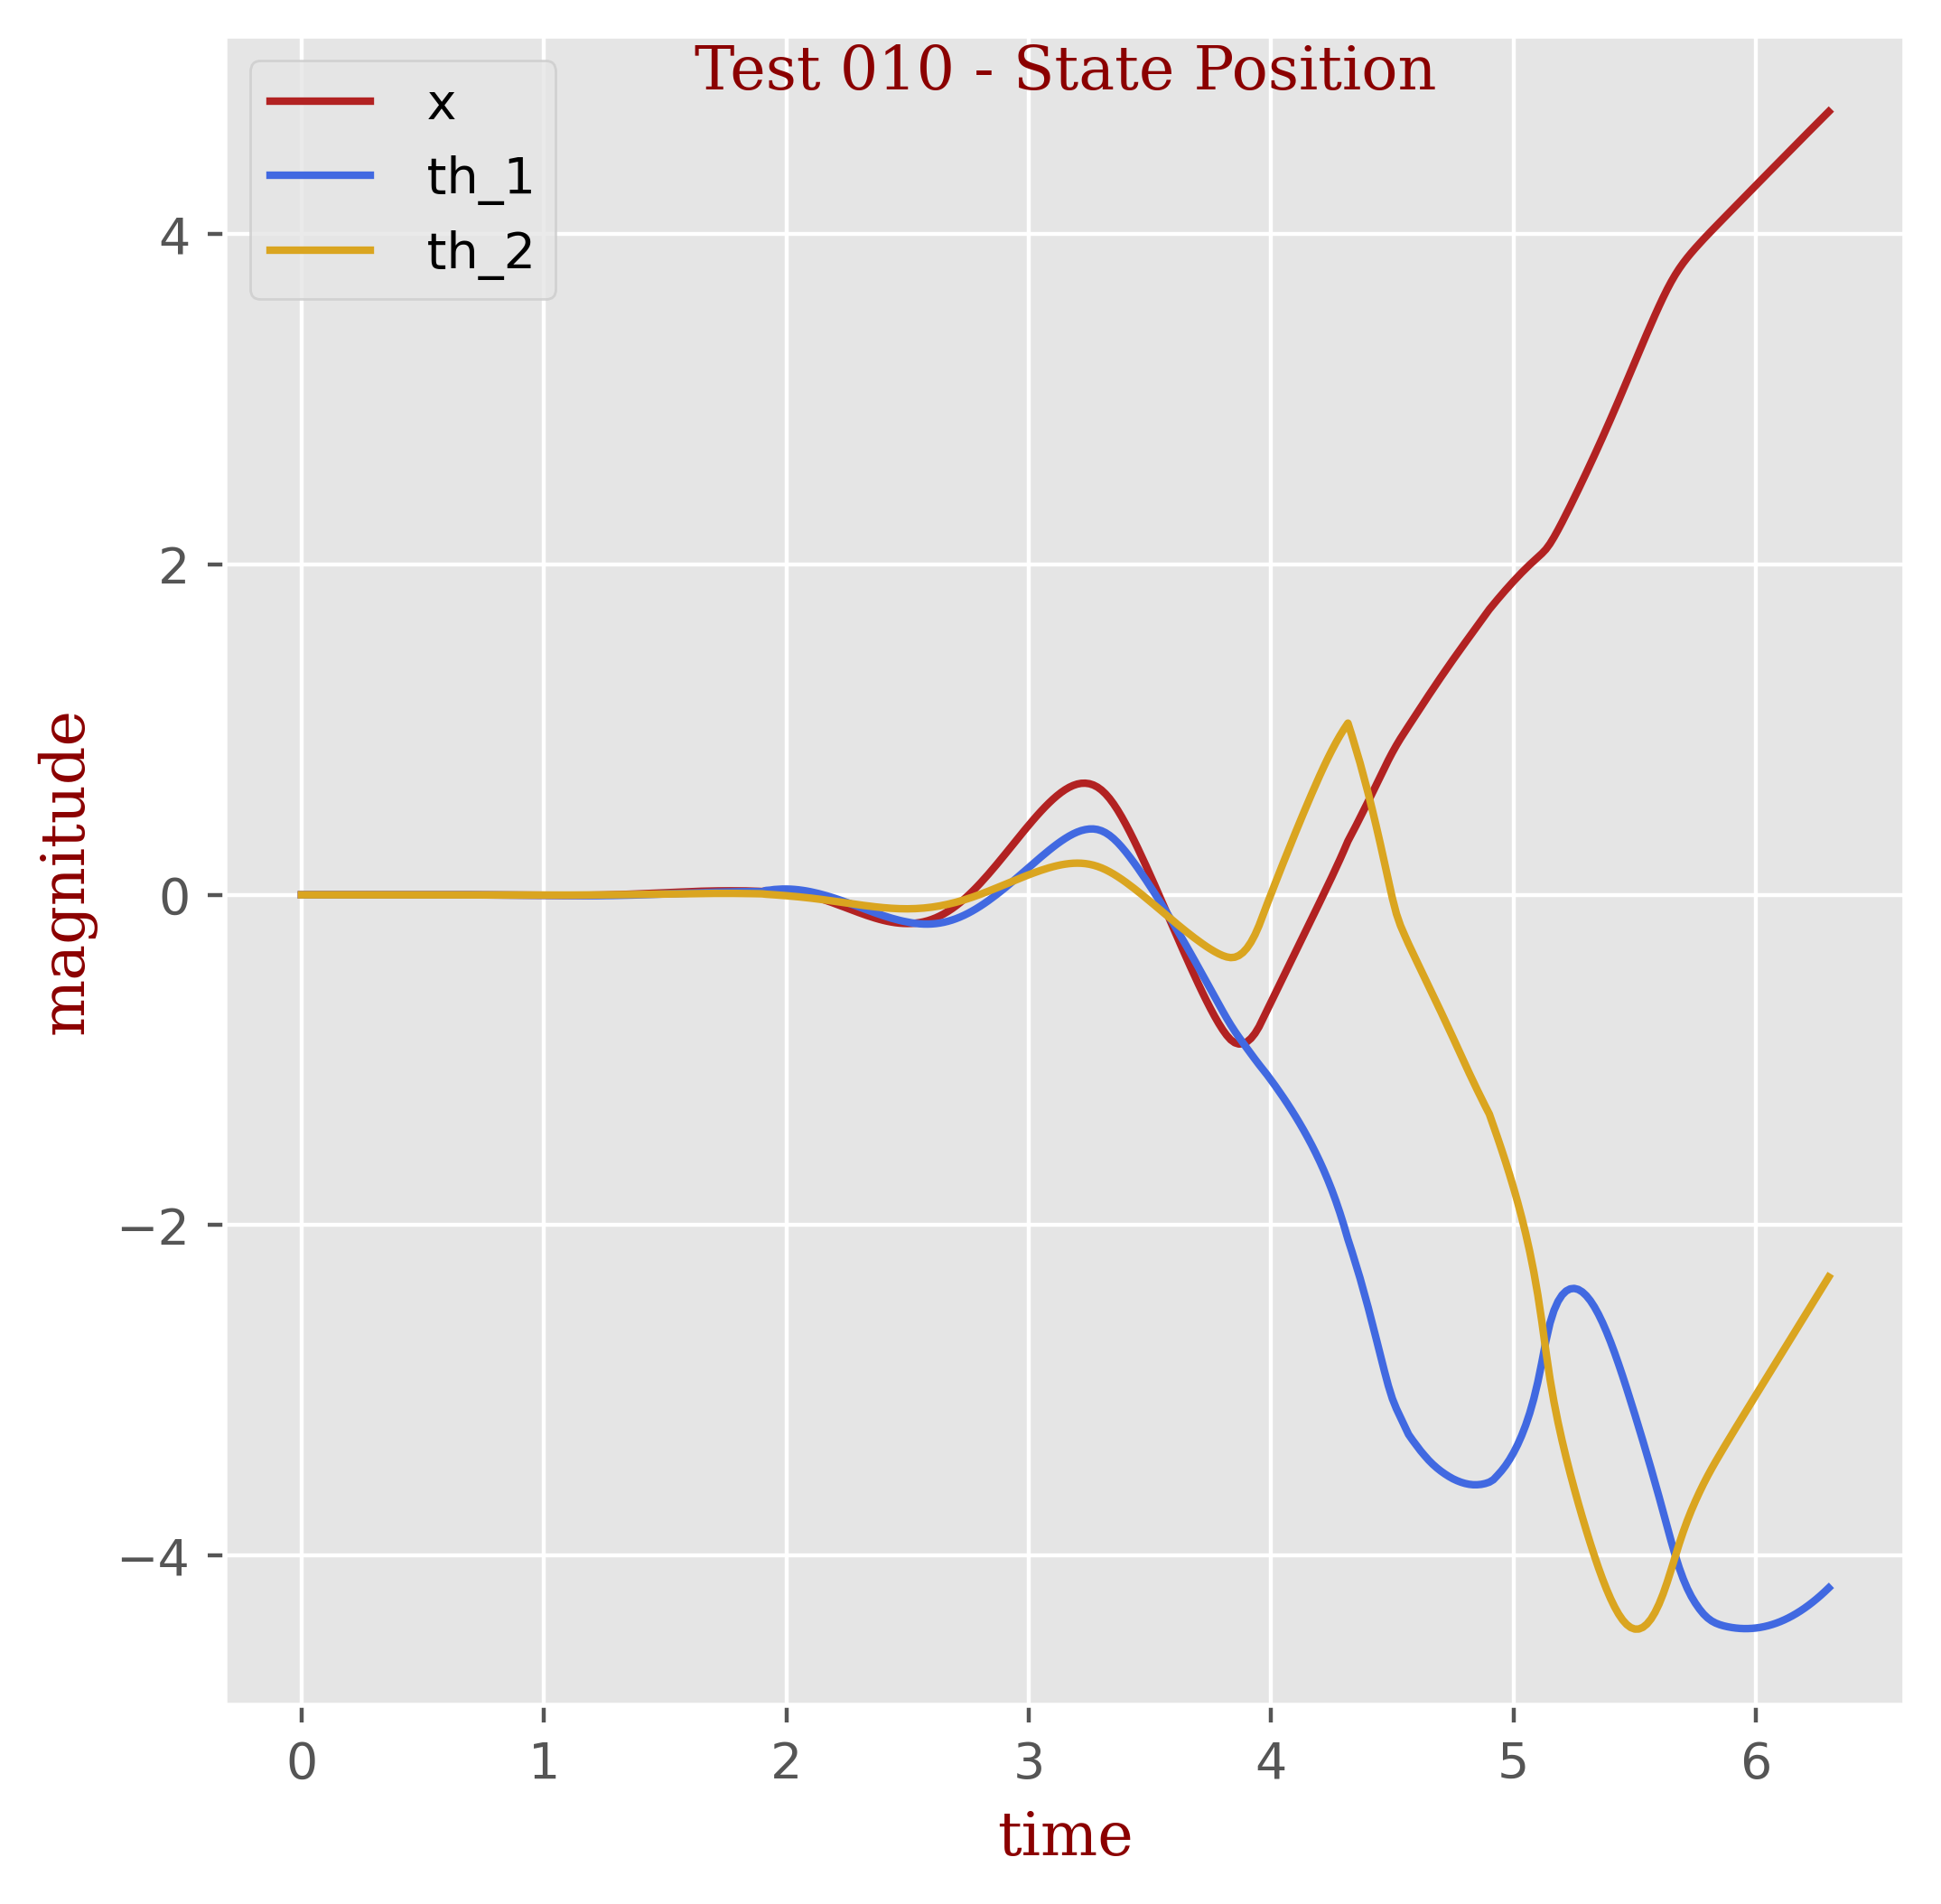
\includegraphics[width=27mm]{Test 010_State_Position.png}}
     \subfigure[\(\dot{q}(t)\)]{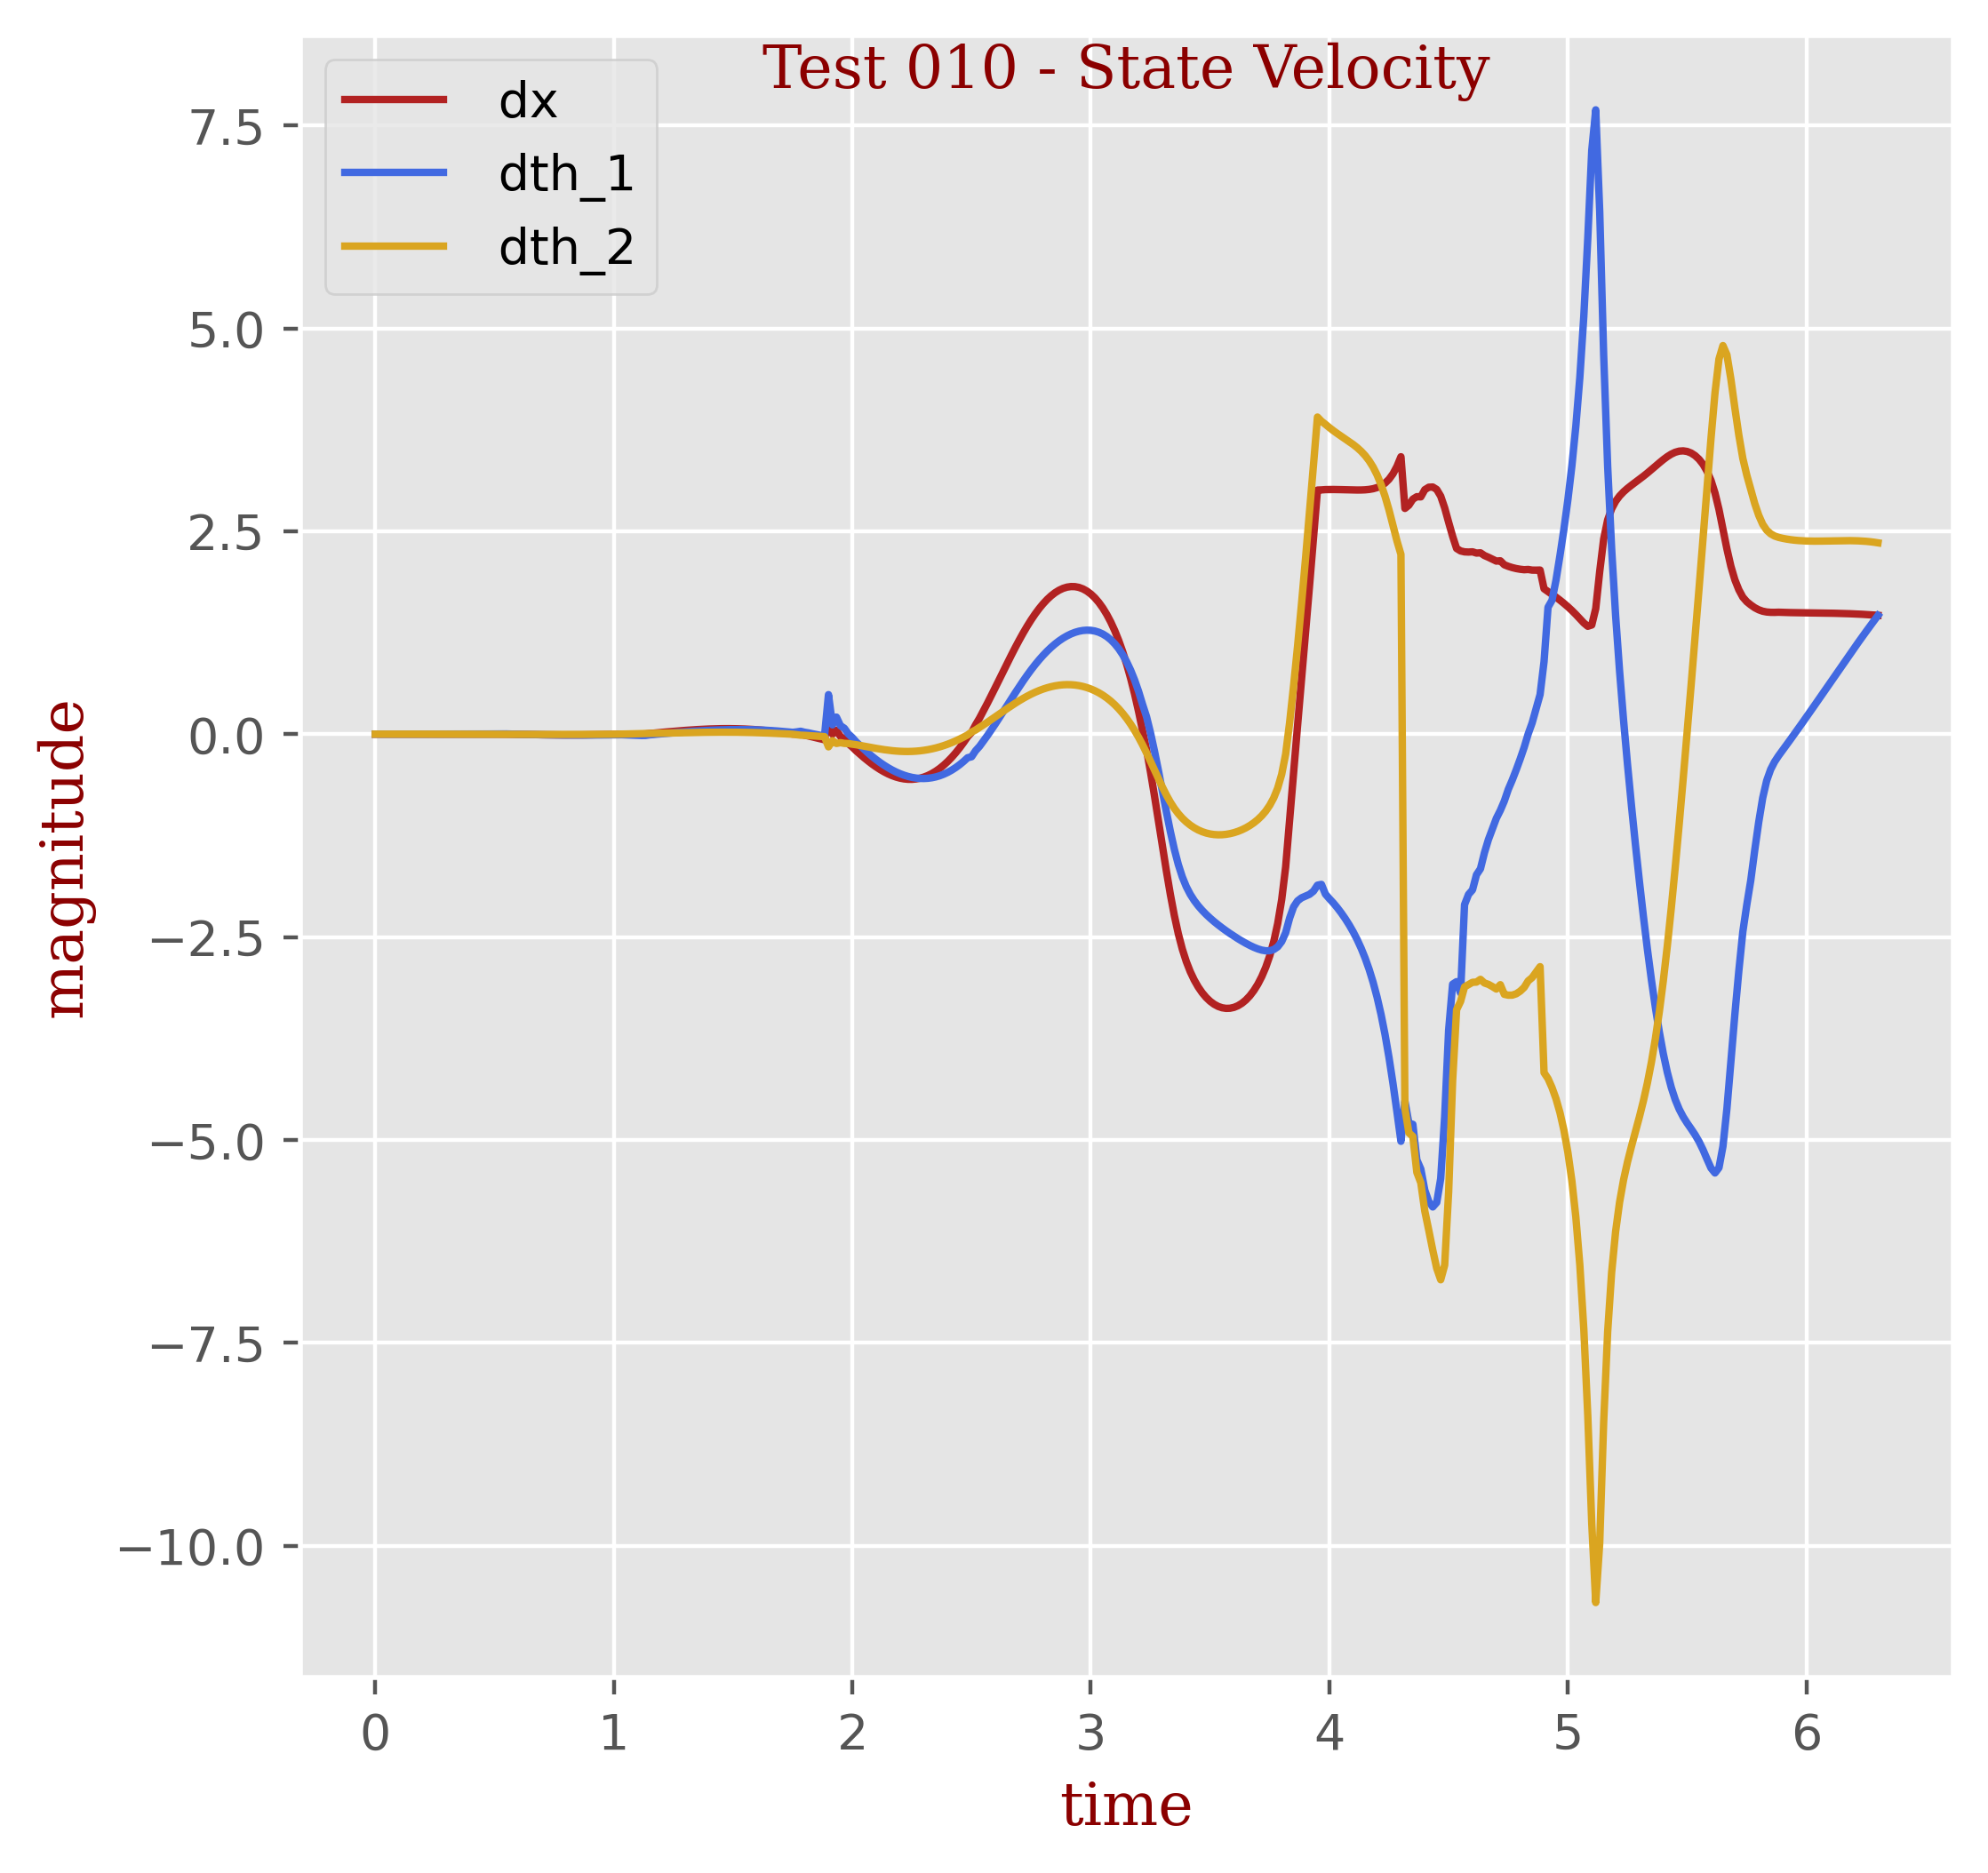
\includegraphics[width=27mm]{Test 010_State_Velocity.png}}
           \subfigure[\(J(t)\)]{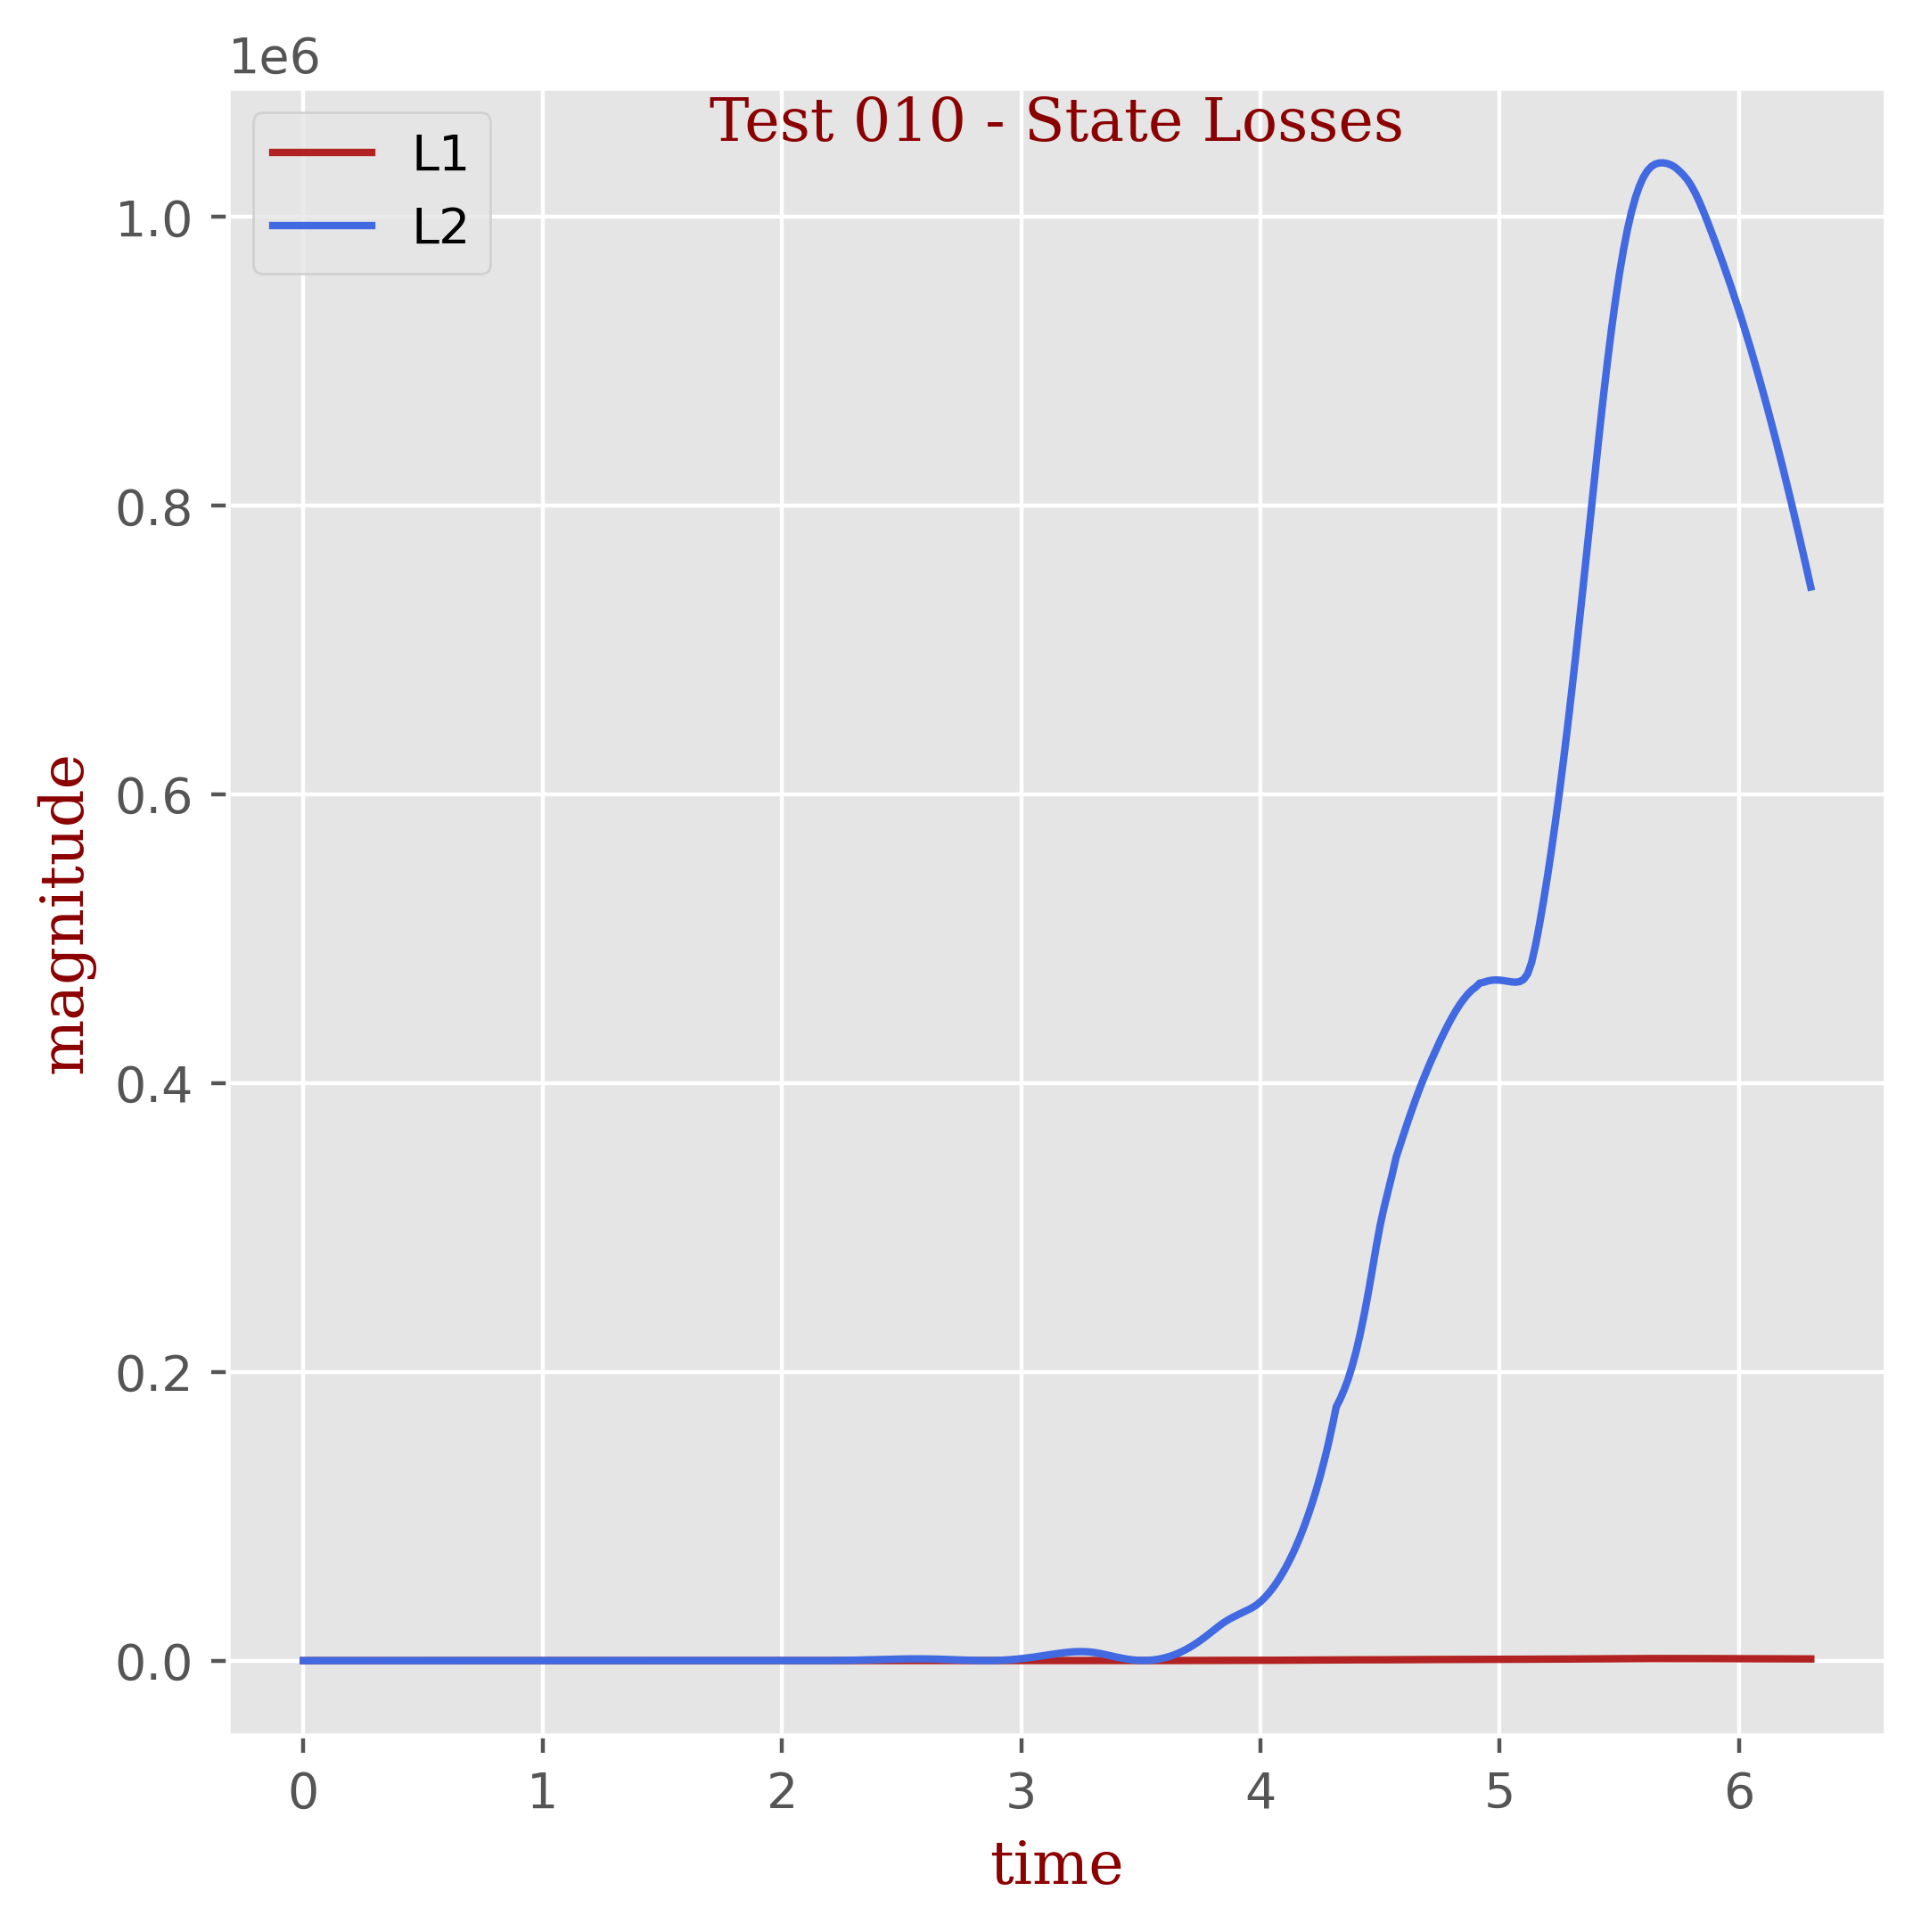
\includegraphics[width=27mm]{Test 010_State_Losses.png}}
                                                    \caption{Test 010}
                                                      \label{fig:t010}
    \end{figure}



    \begin{figure}
        \centering
               \subfigure[\(q(t)\)]{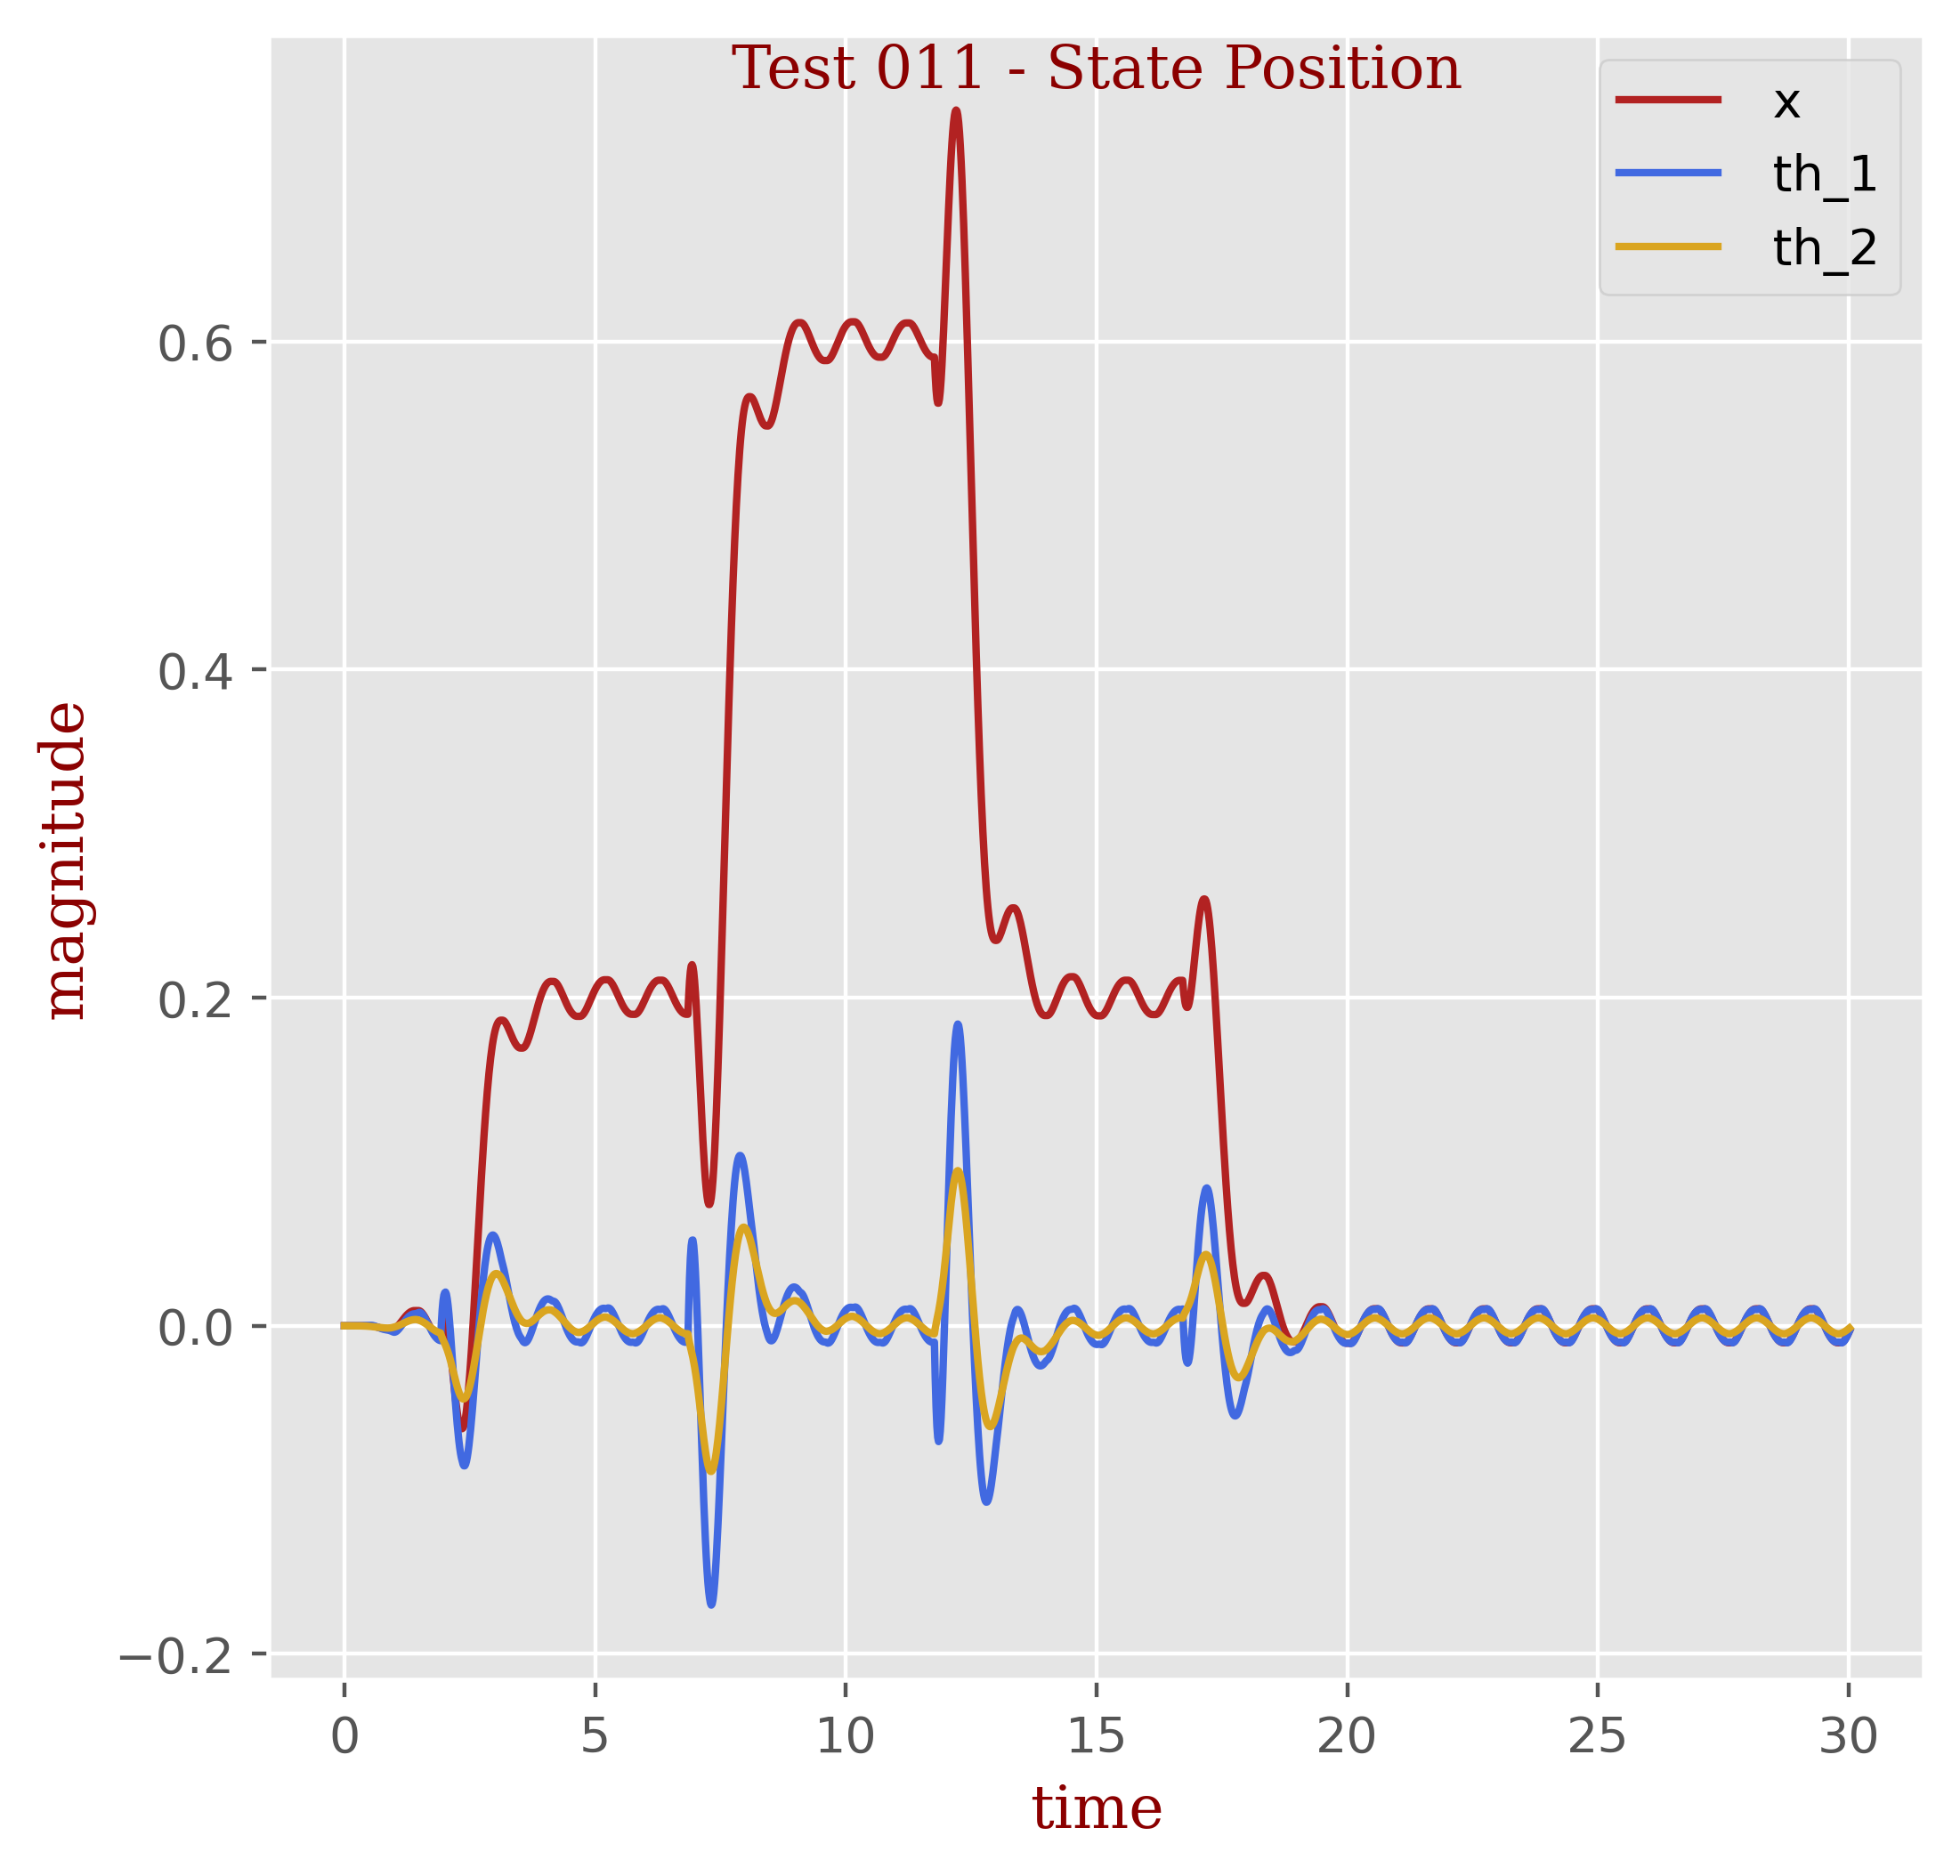
\includegraphics[width=27mm]{Test 011_State_Position.png}}
         \subfigure[\(\dot{q}(t)\)]{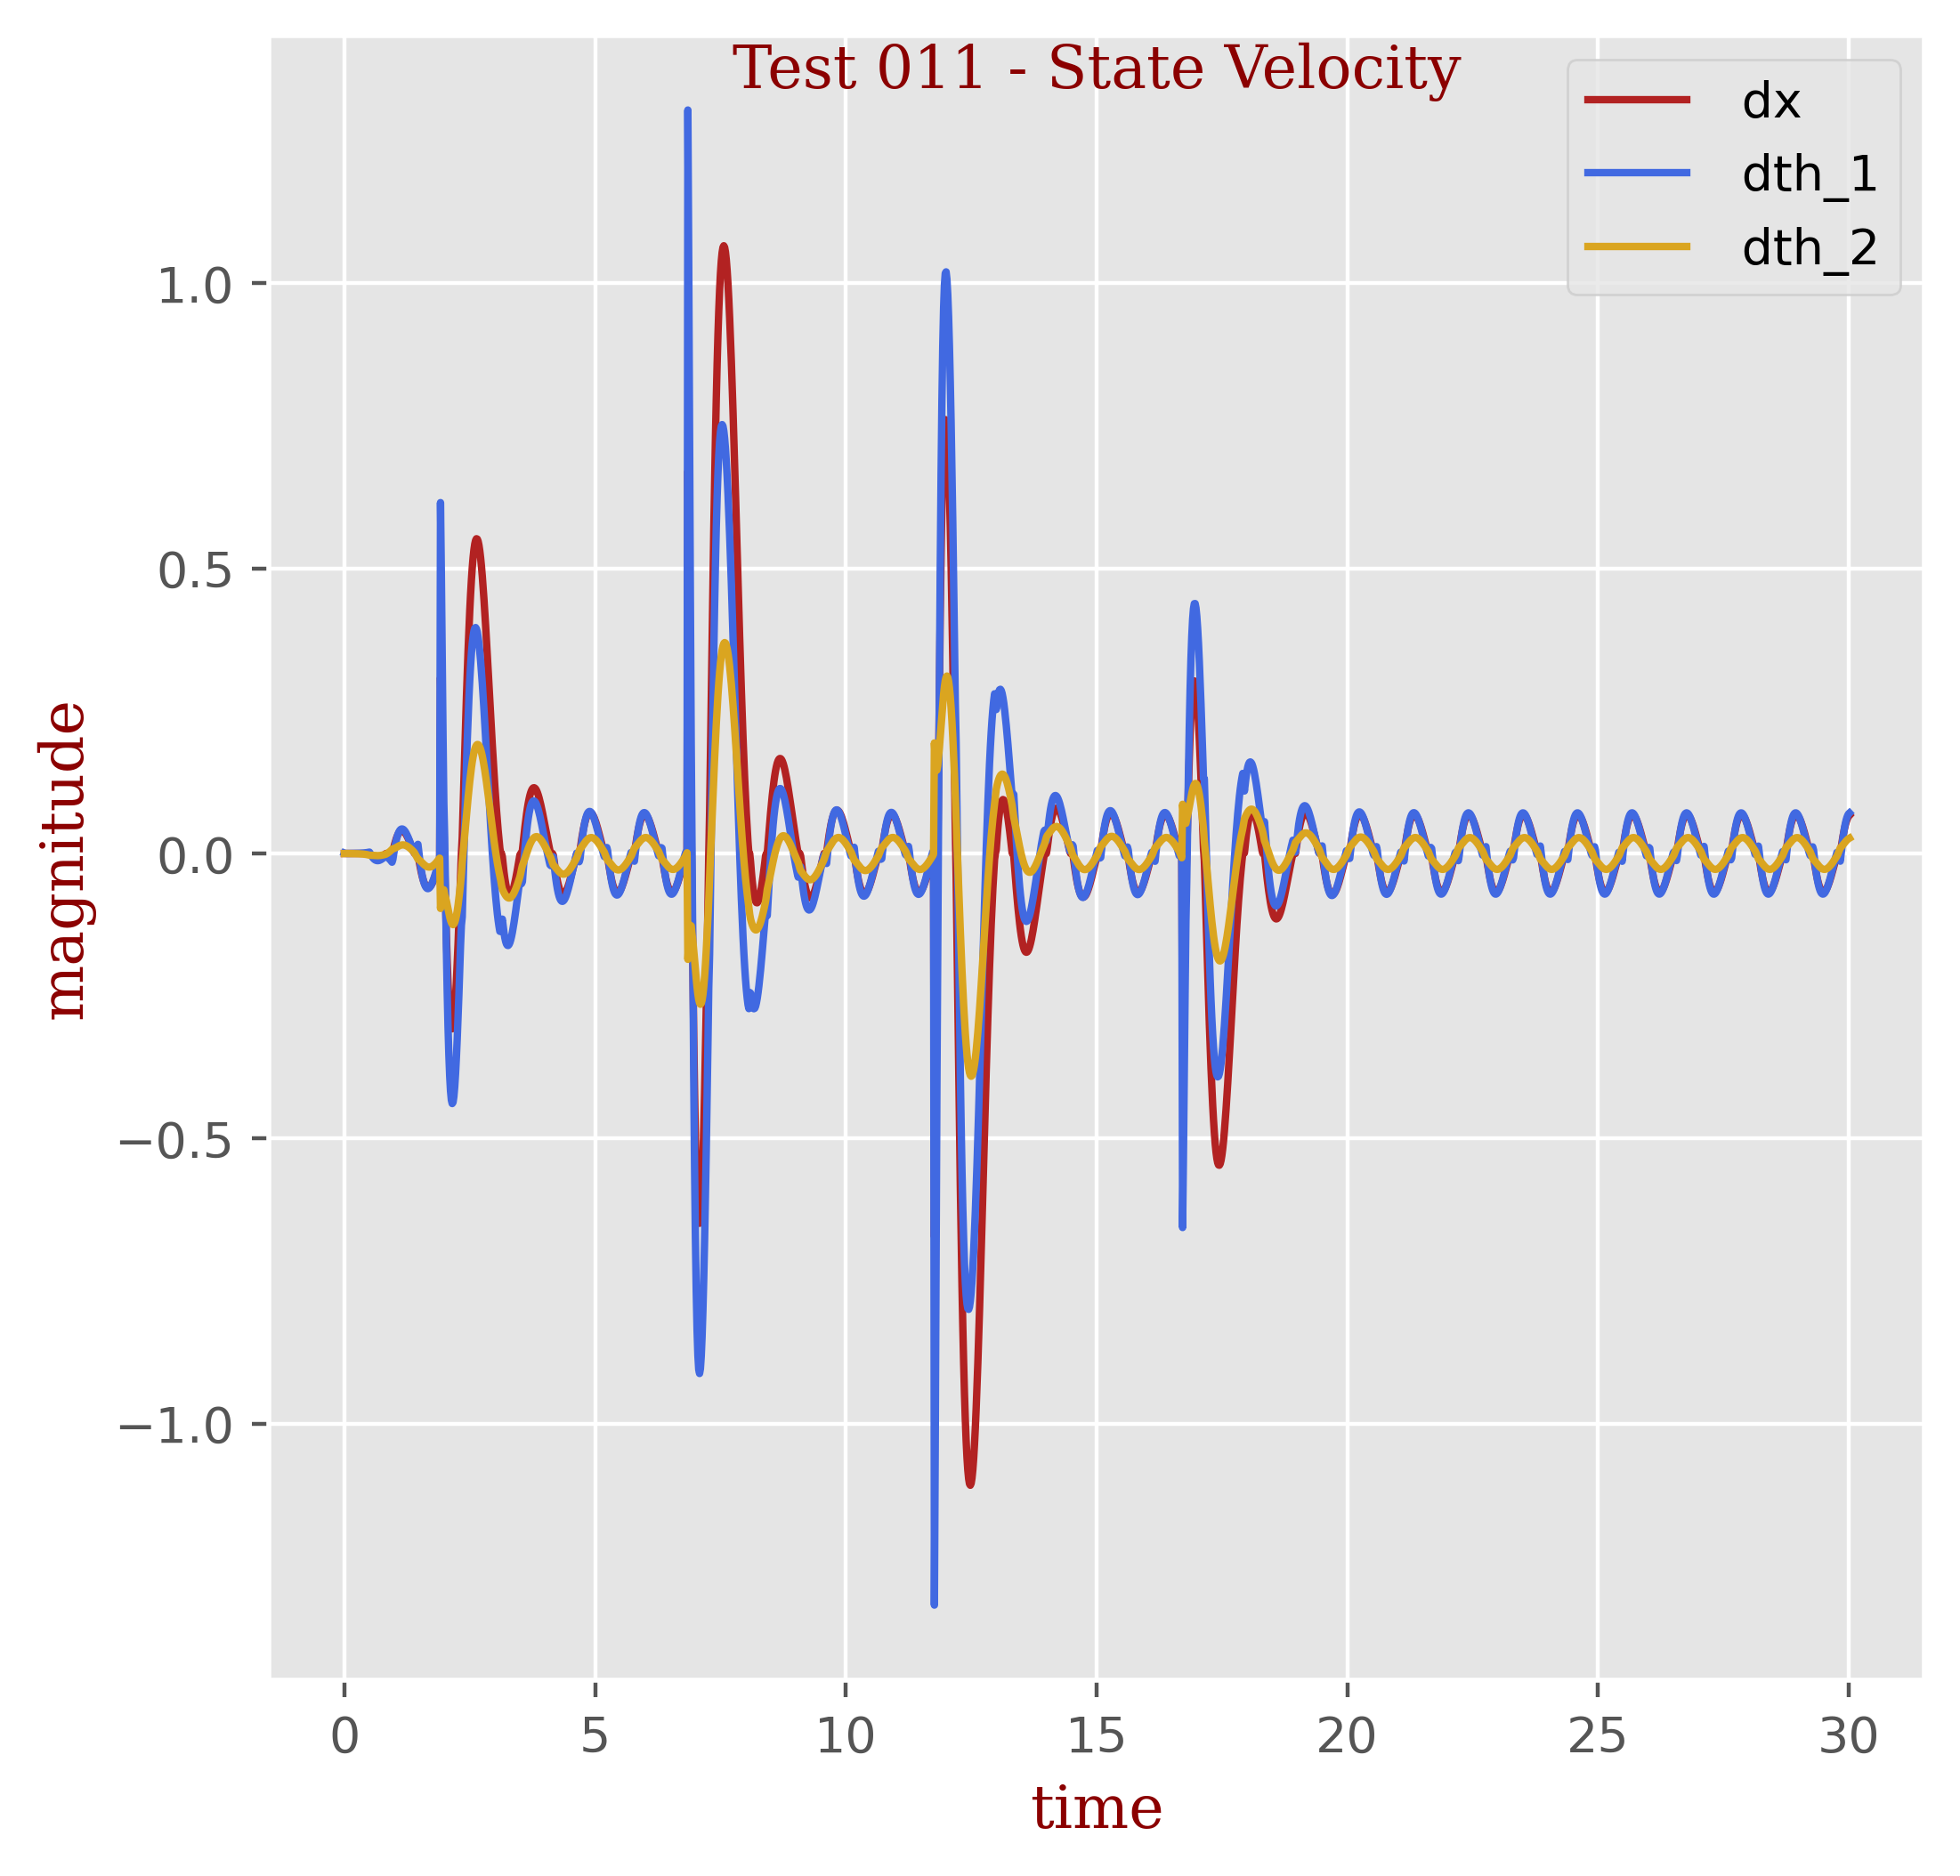
\includegraphics[width=27mm]{Test 011_State_Velocity.png}}
               \subfigure[\(J(t)\)]{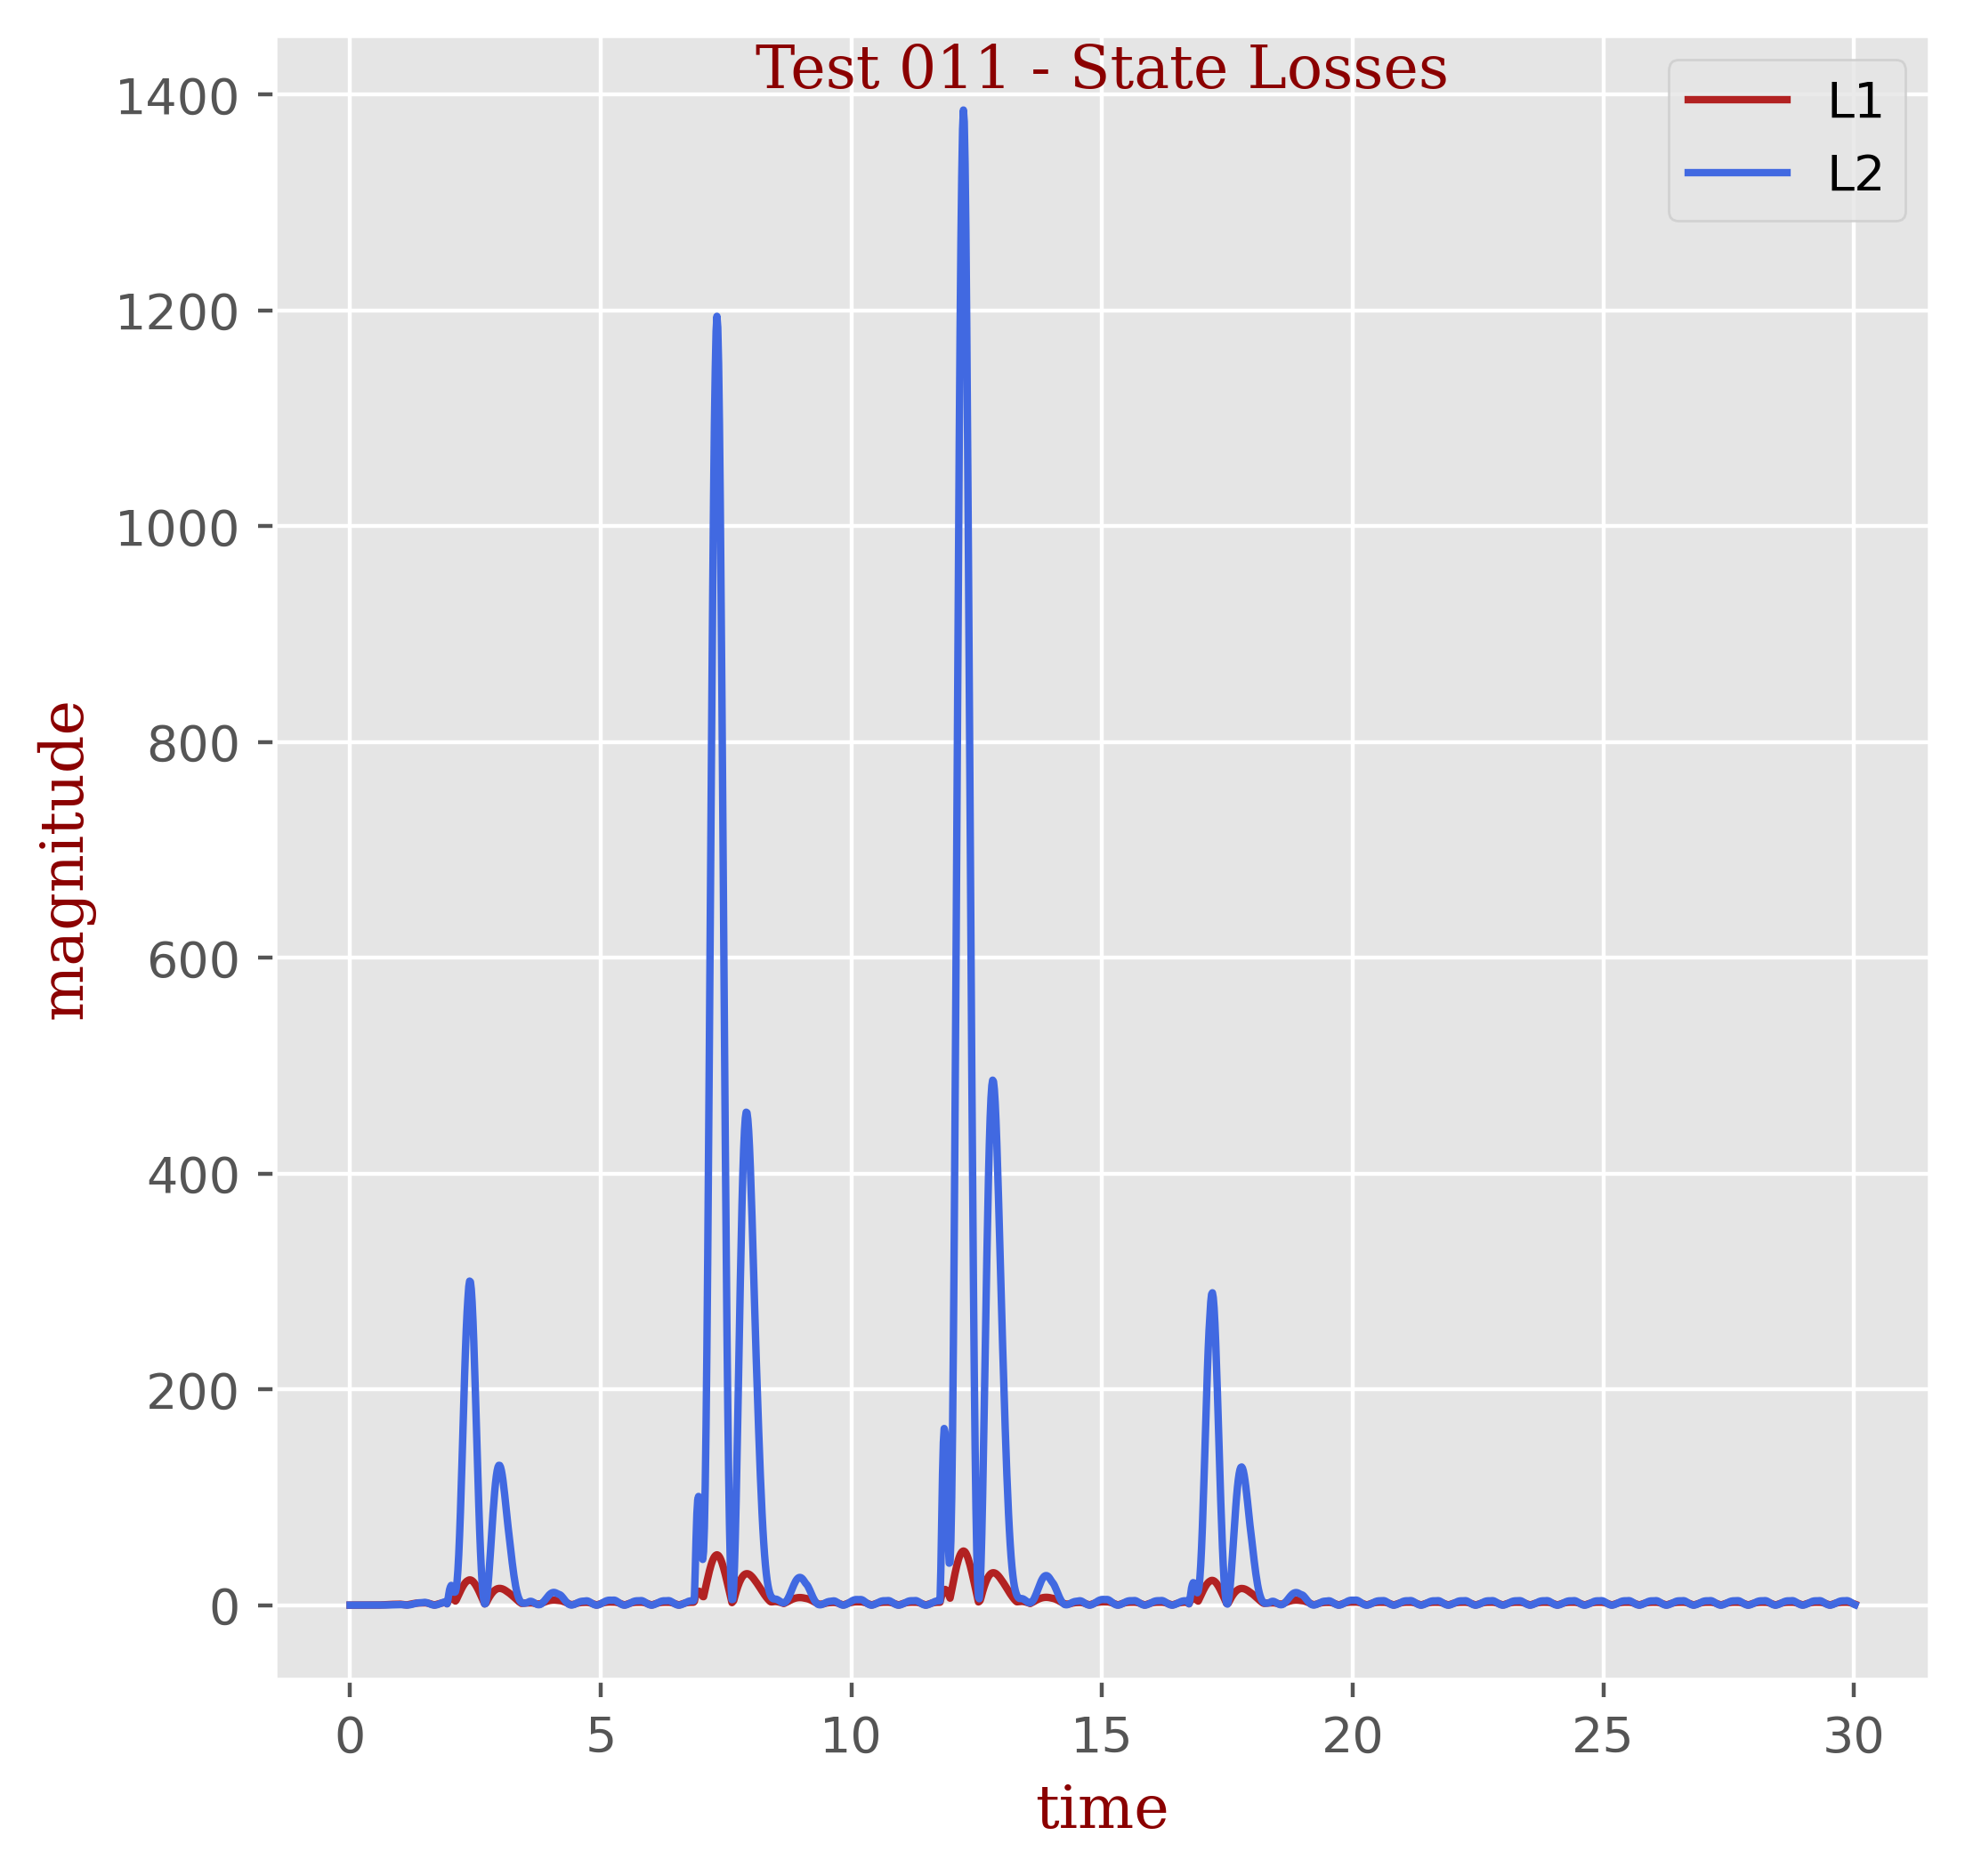
\includegraphics[width=27mm]{Test 011_State_Losses.png}}
                                                        \caption{Test 011}
                                                          \label{fig:t011}
        \end{figure}



\begin{figure}
    \centering
          \subfigure[\(q(t)\)]{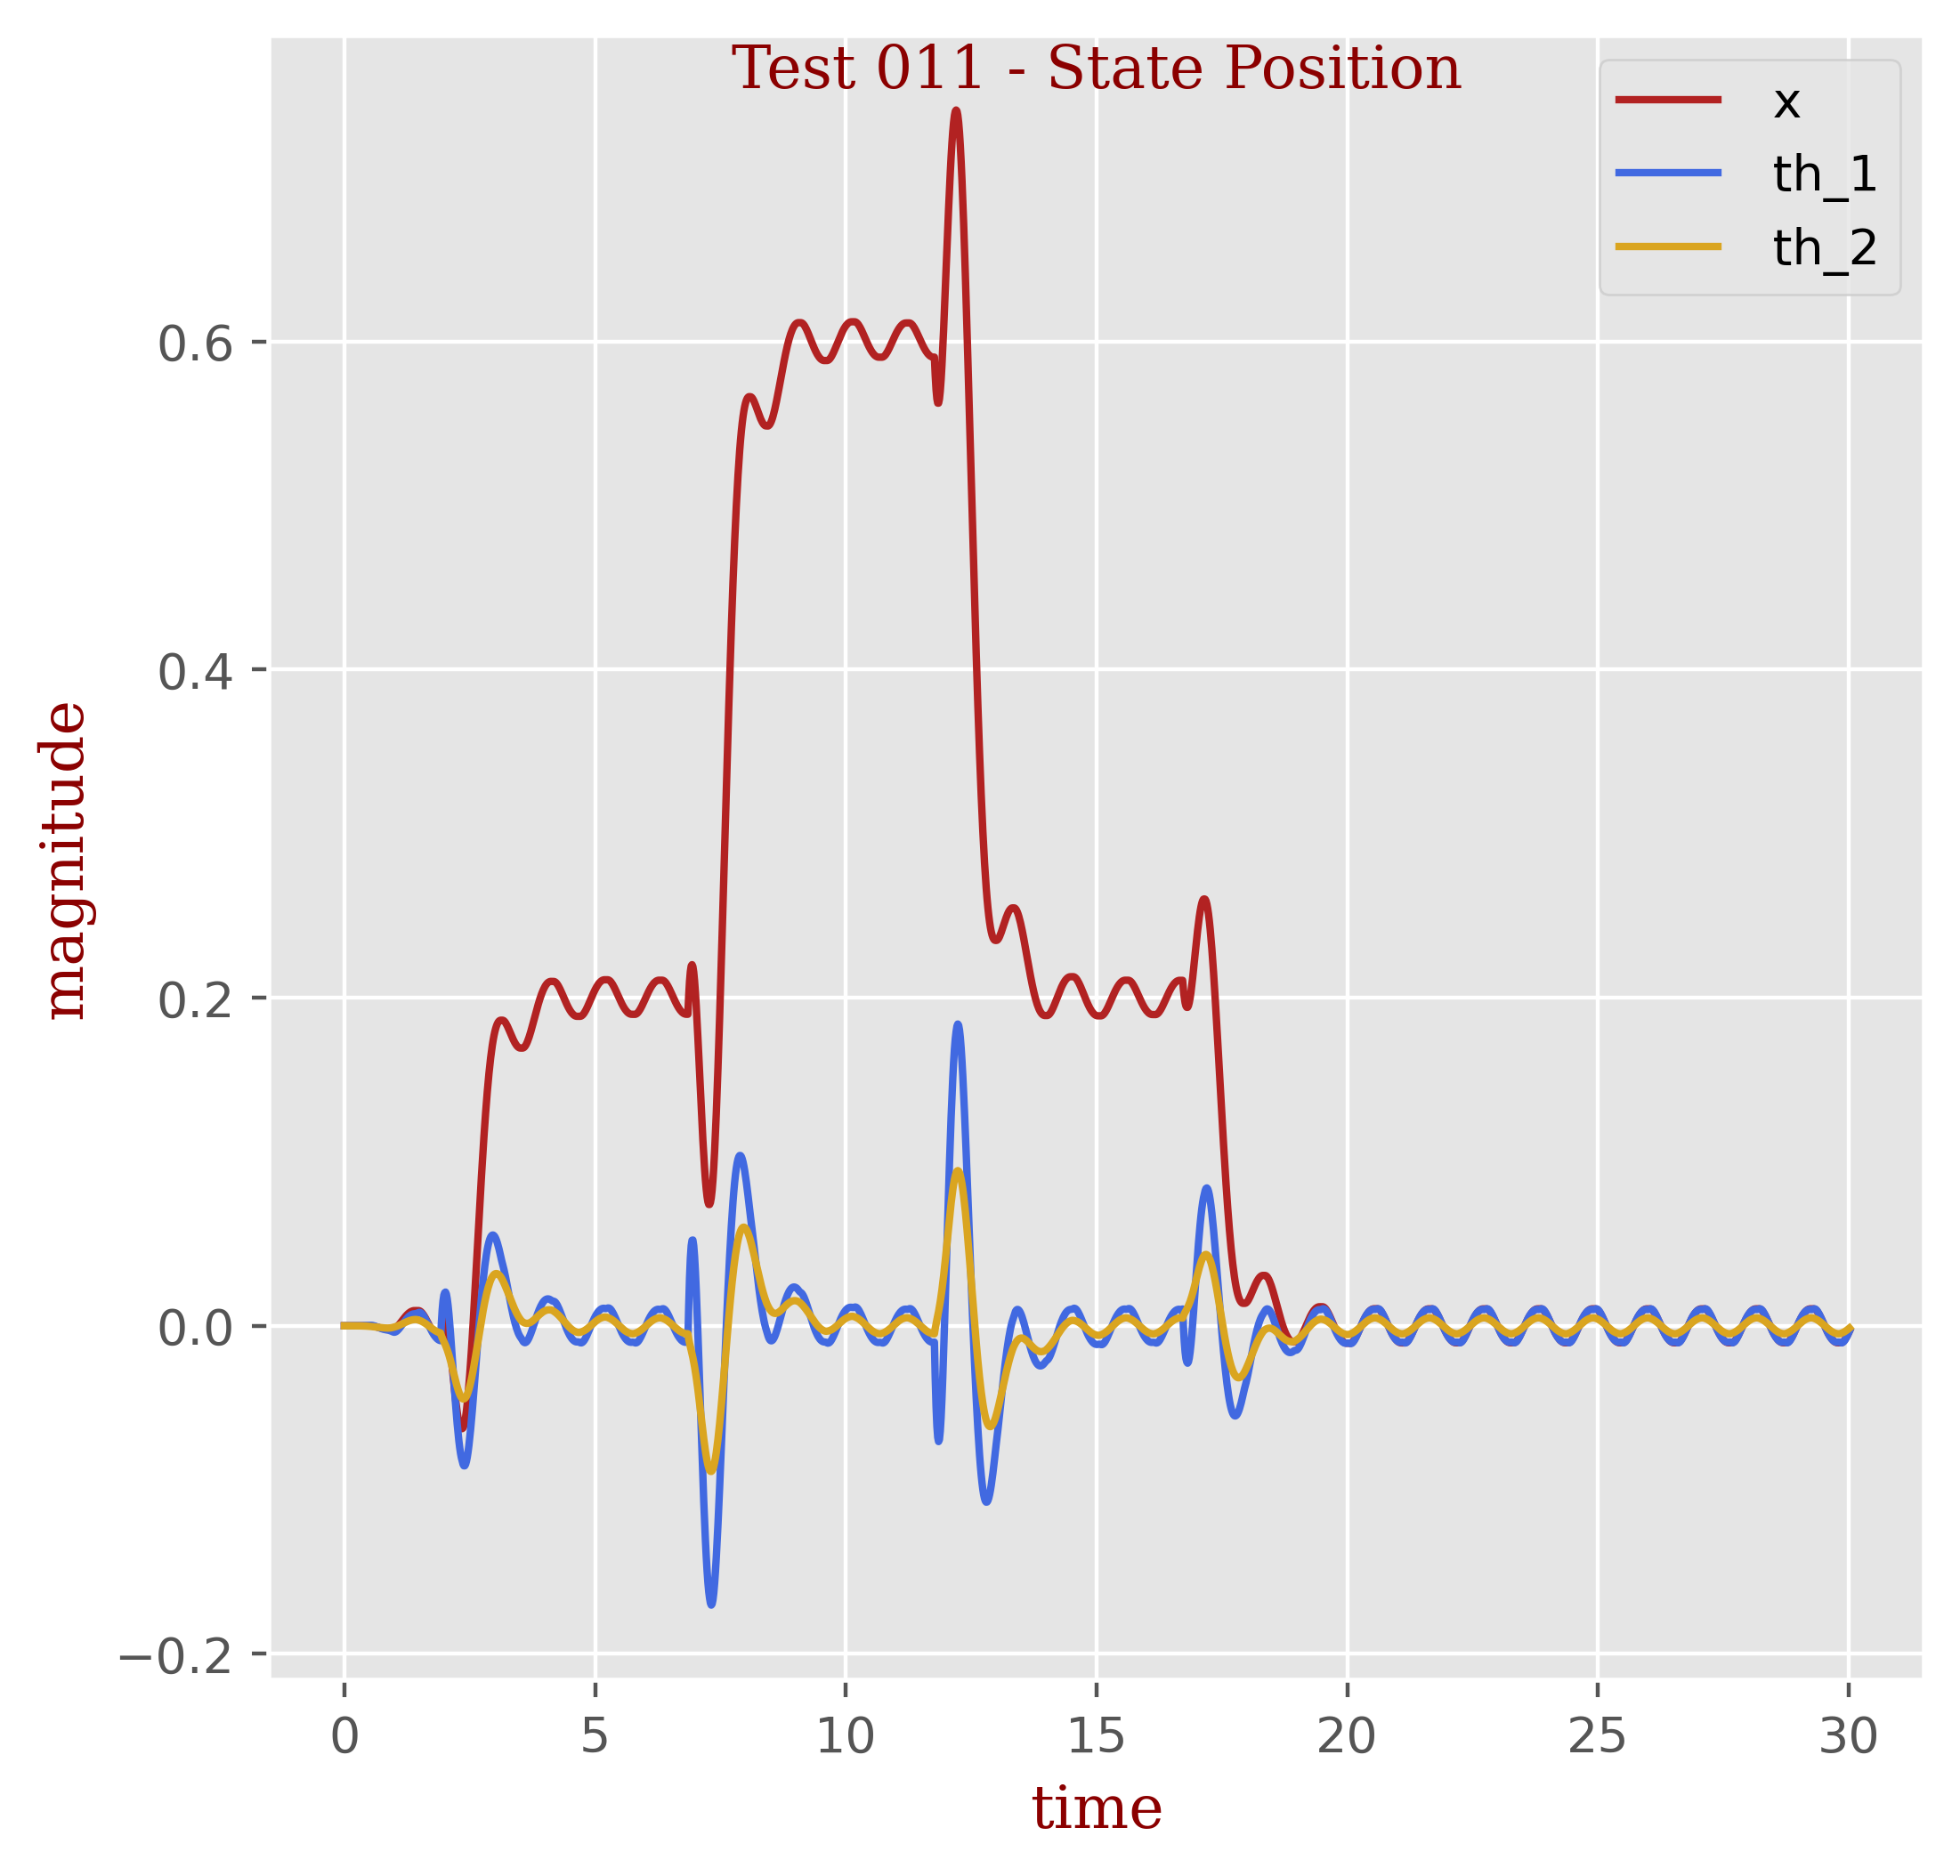
\includegraphics[width=27mm]{Test 011_State_Position.png}}
    \subfigure[\(\dot{q}(t)\)]{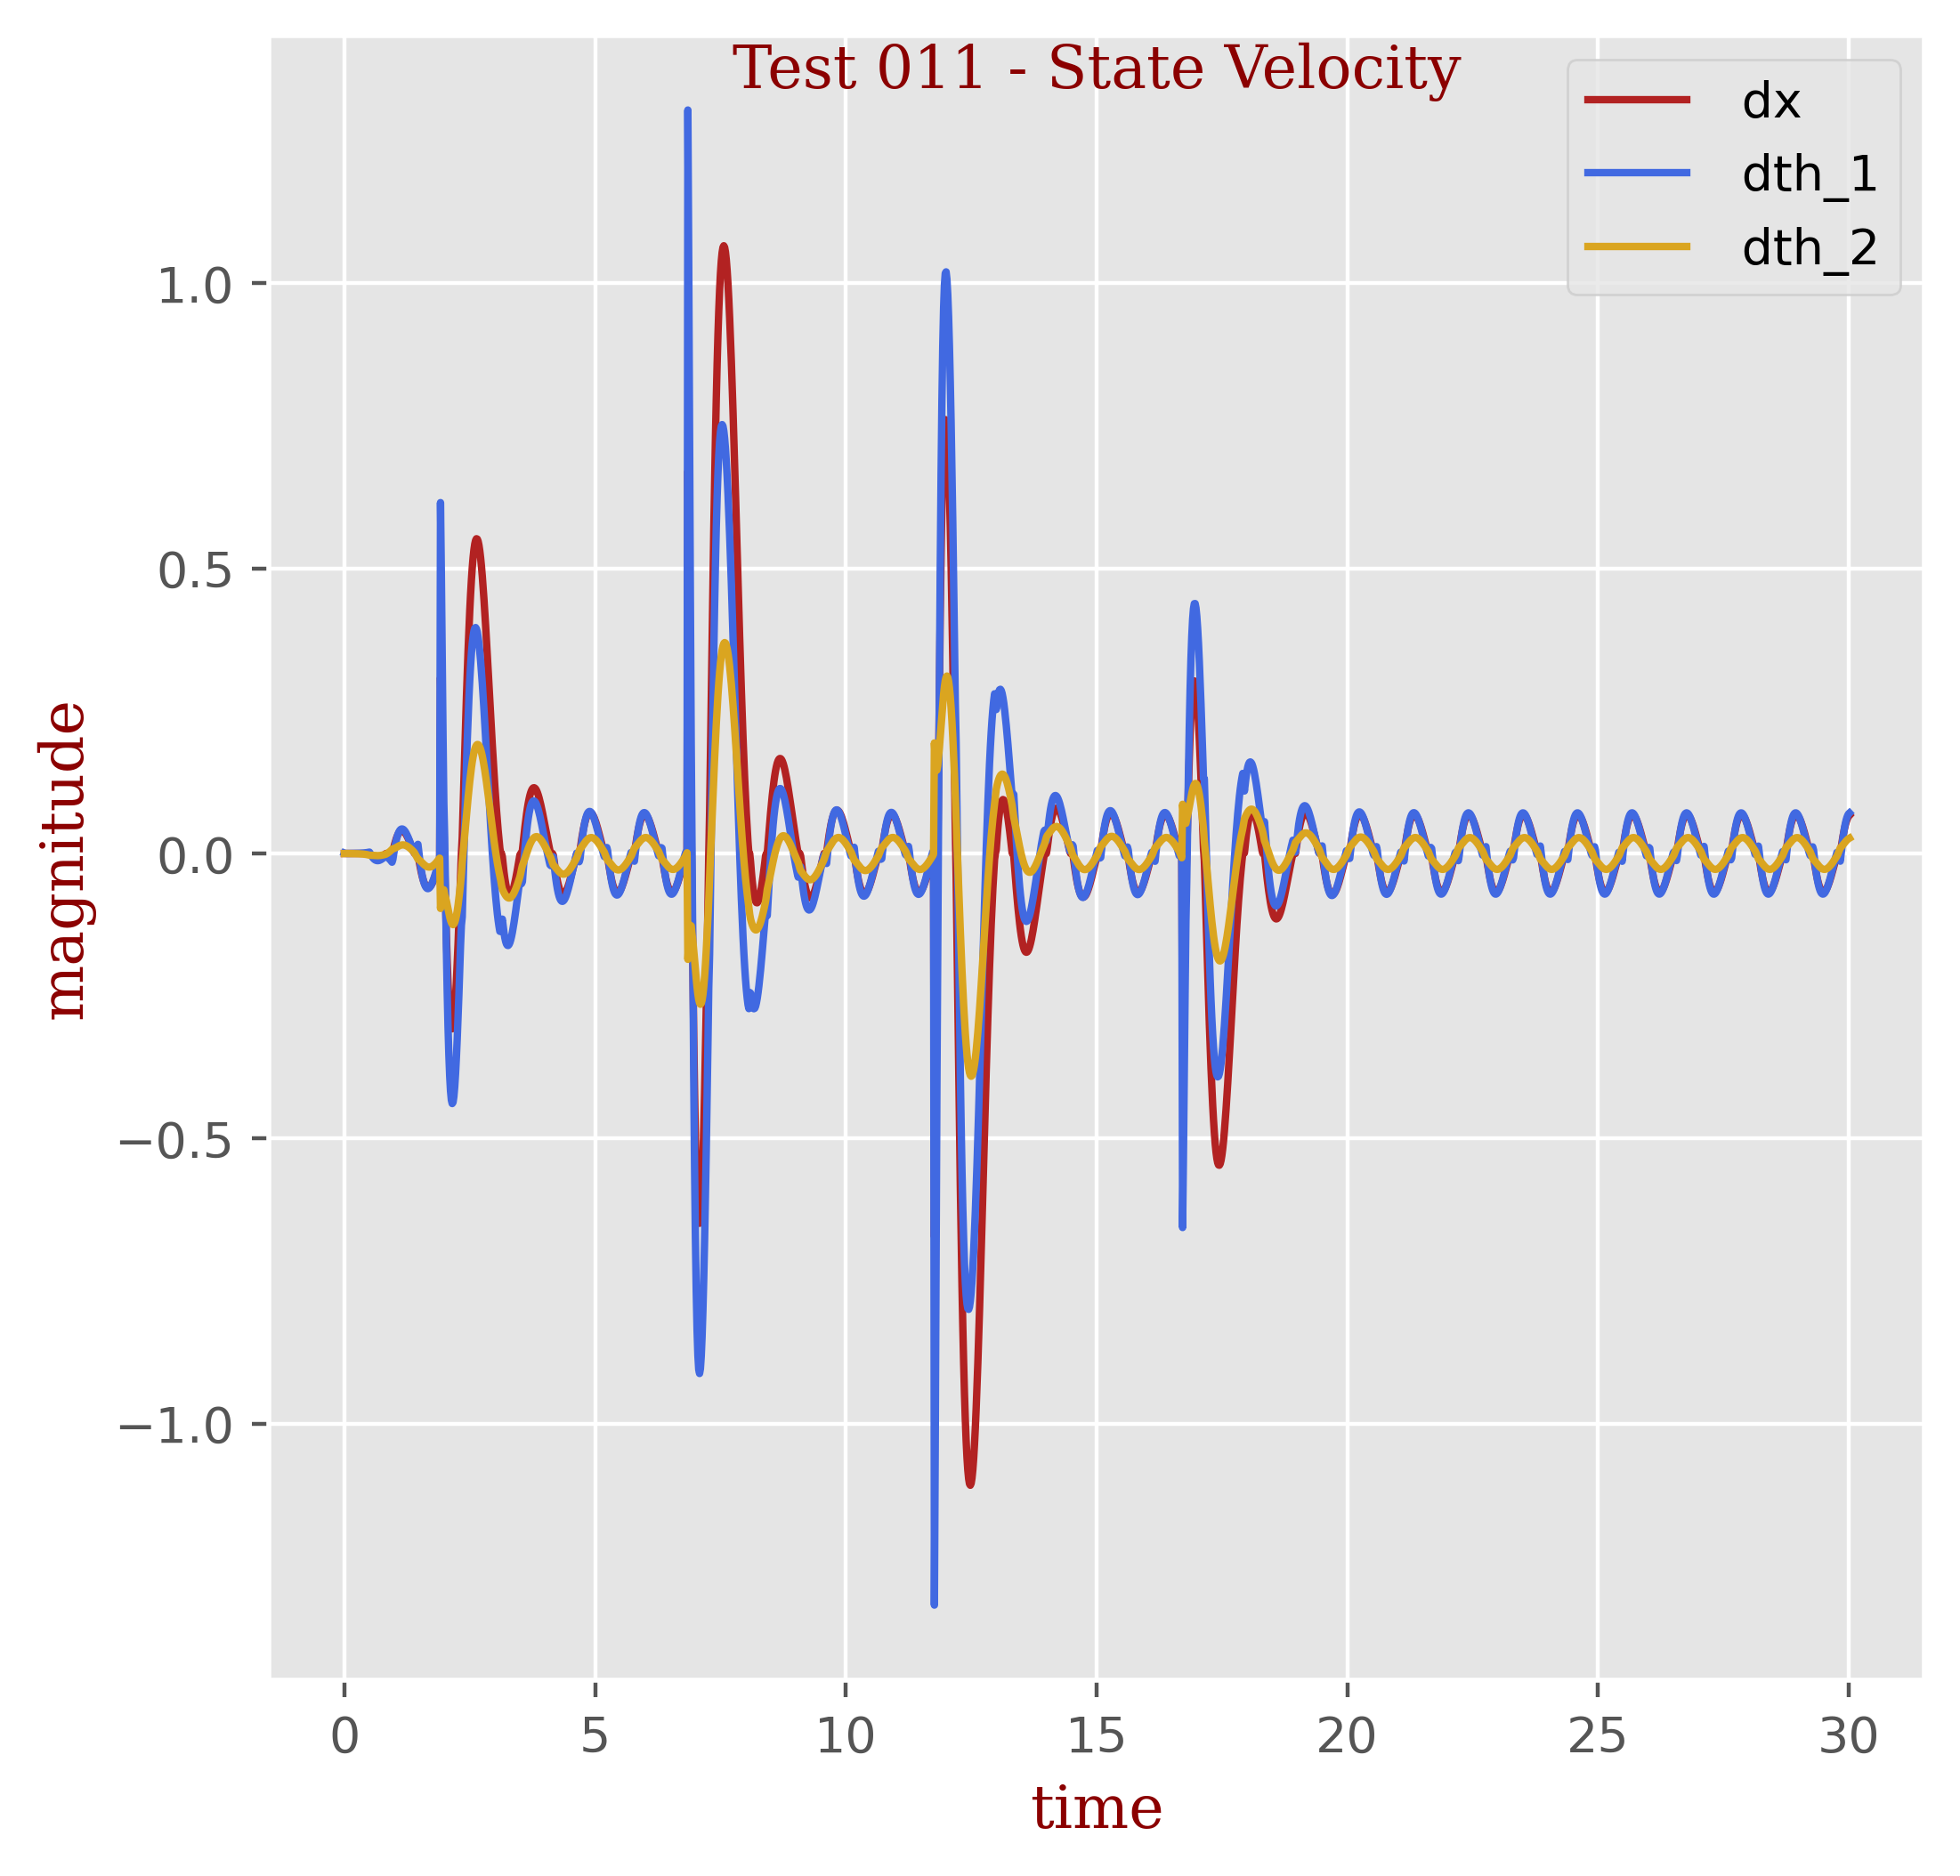
\includegraphics[width=27mm]{Test 011_State_Velocity.png}}
          \subfigure[\(J(t)\)]{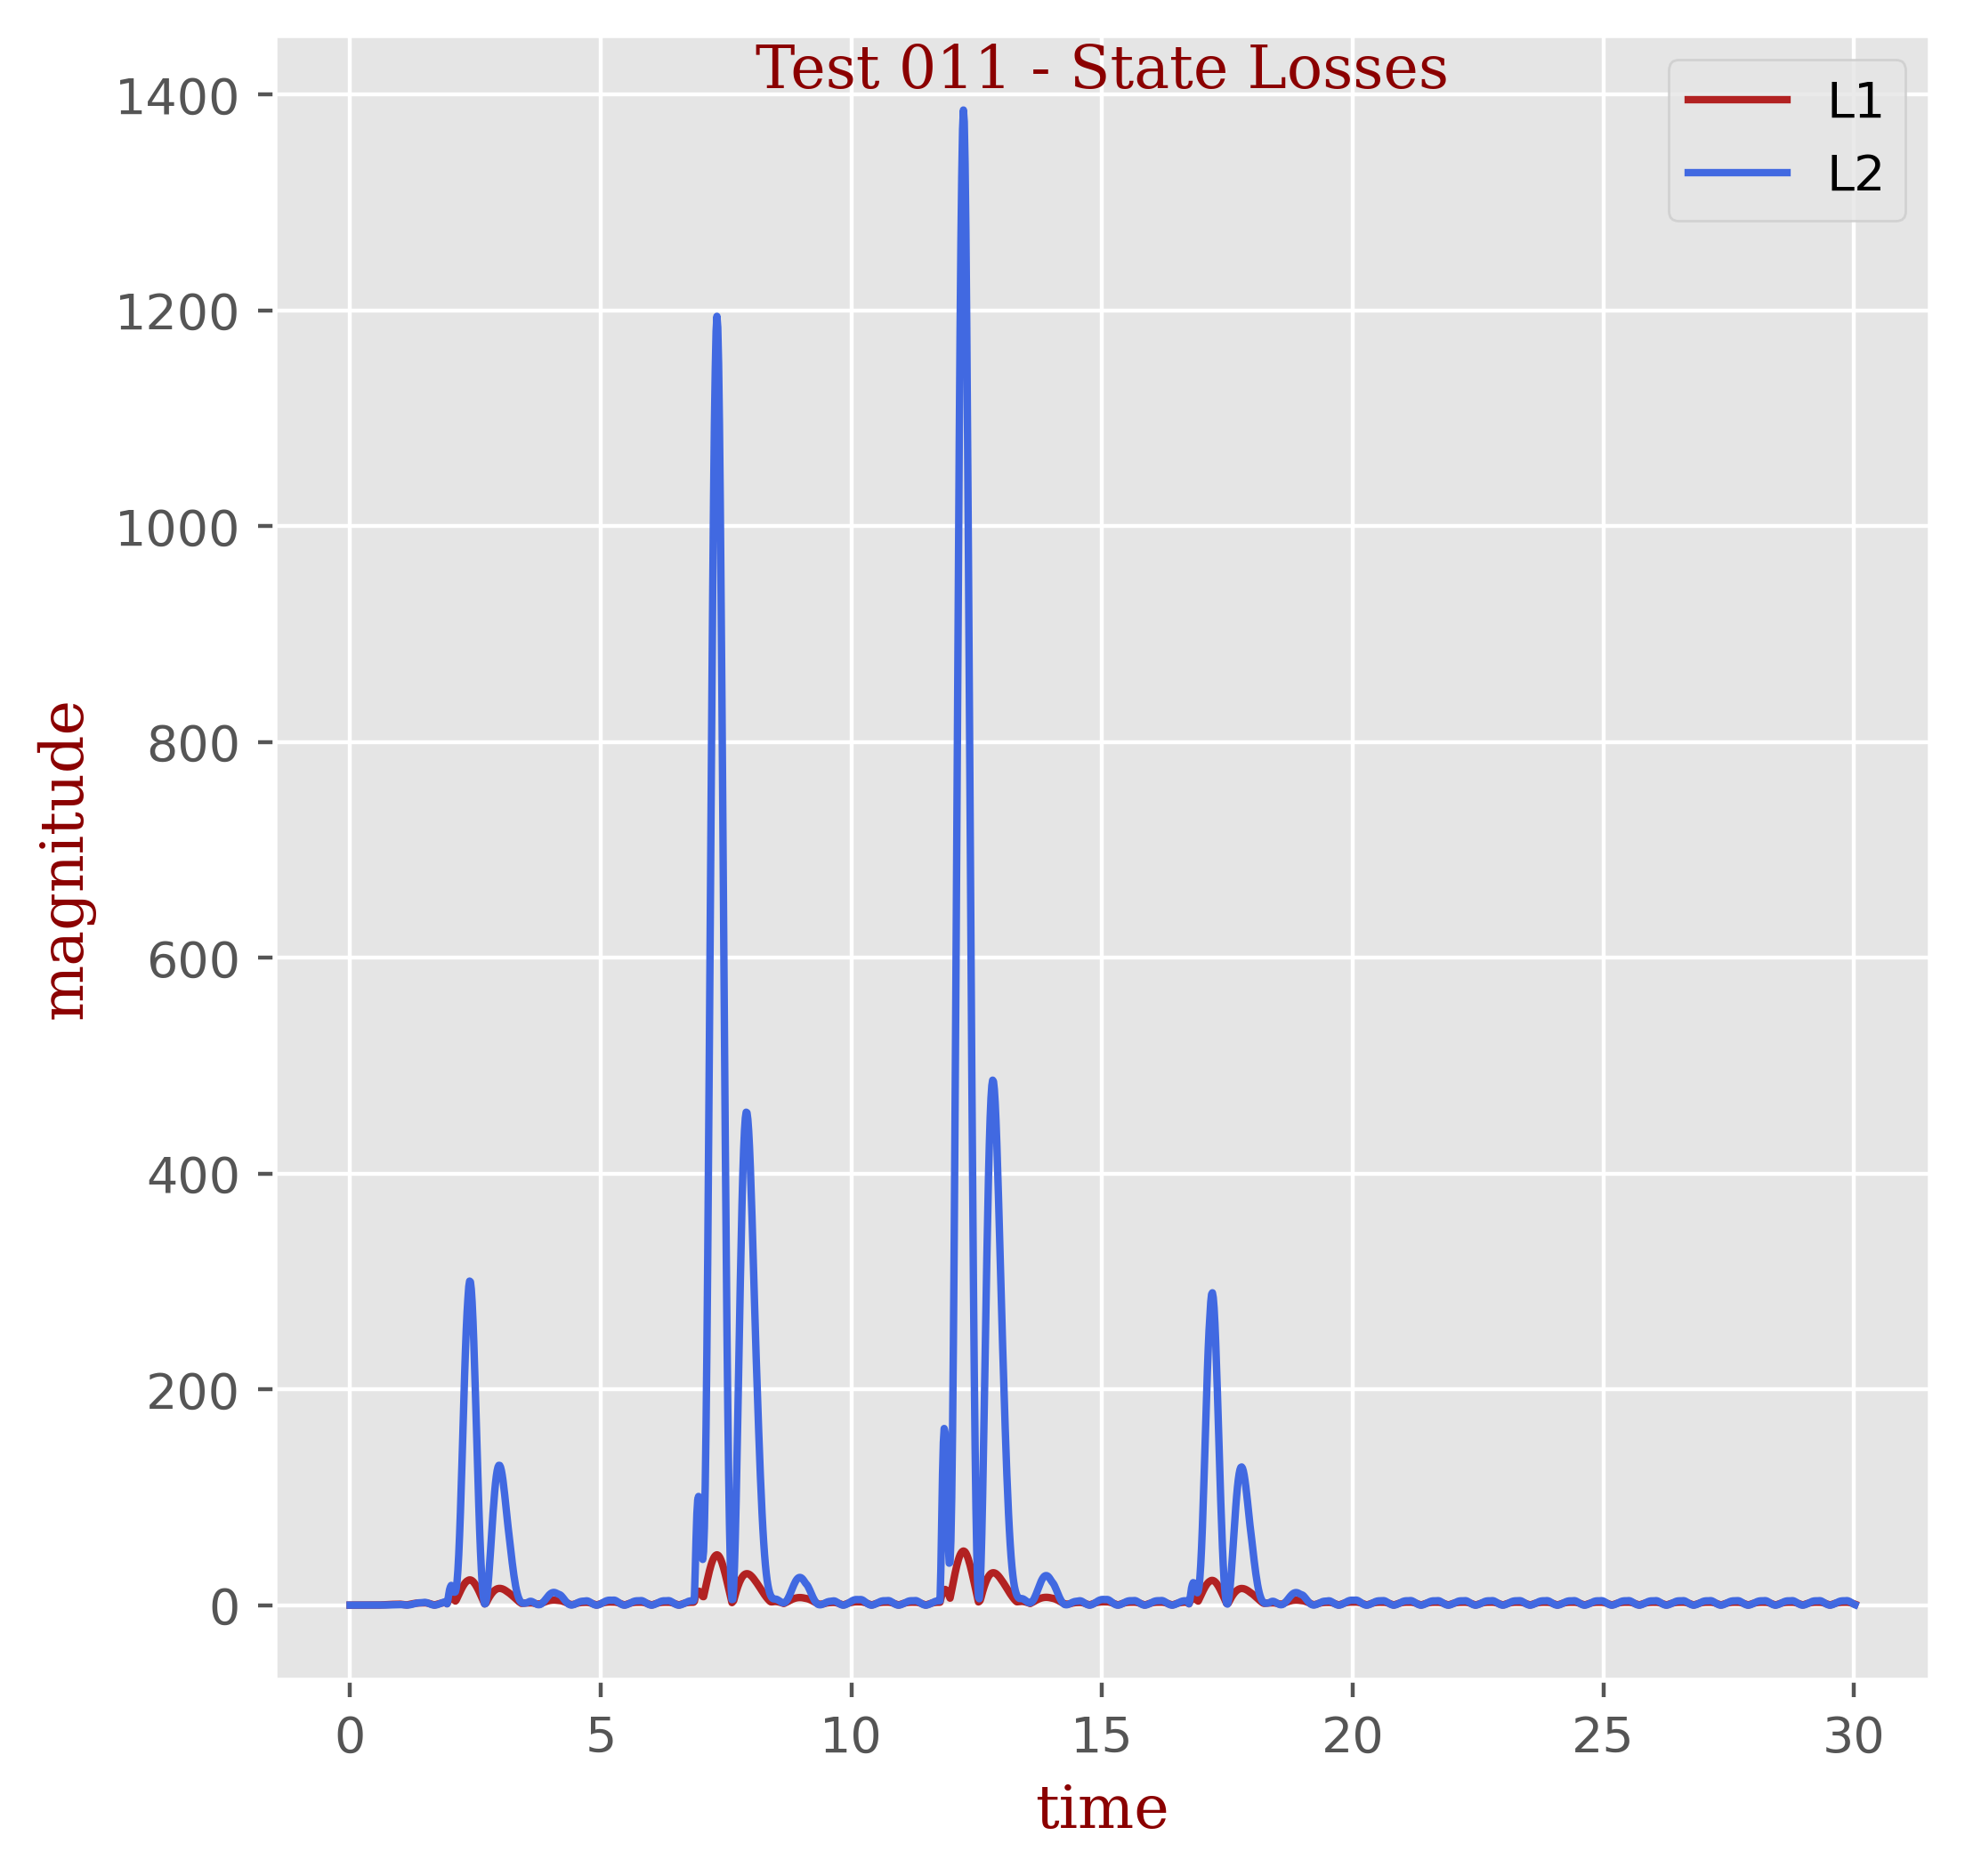
\includegraphics[width=27mm]{Test 011_State_Losses.png}}
                                                   \caption{Test 011}
                                                     \label{fig:t011}
    \end{figure}


    \begin{figure}
        \centering
              \subfigure[\(q(t)\)]{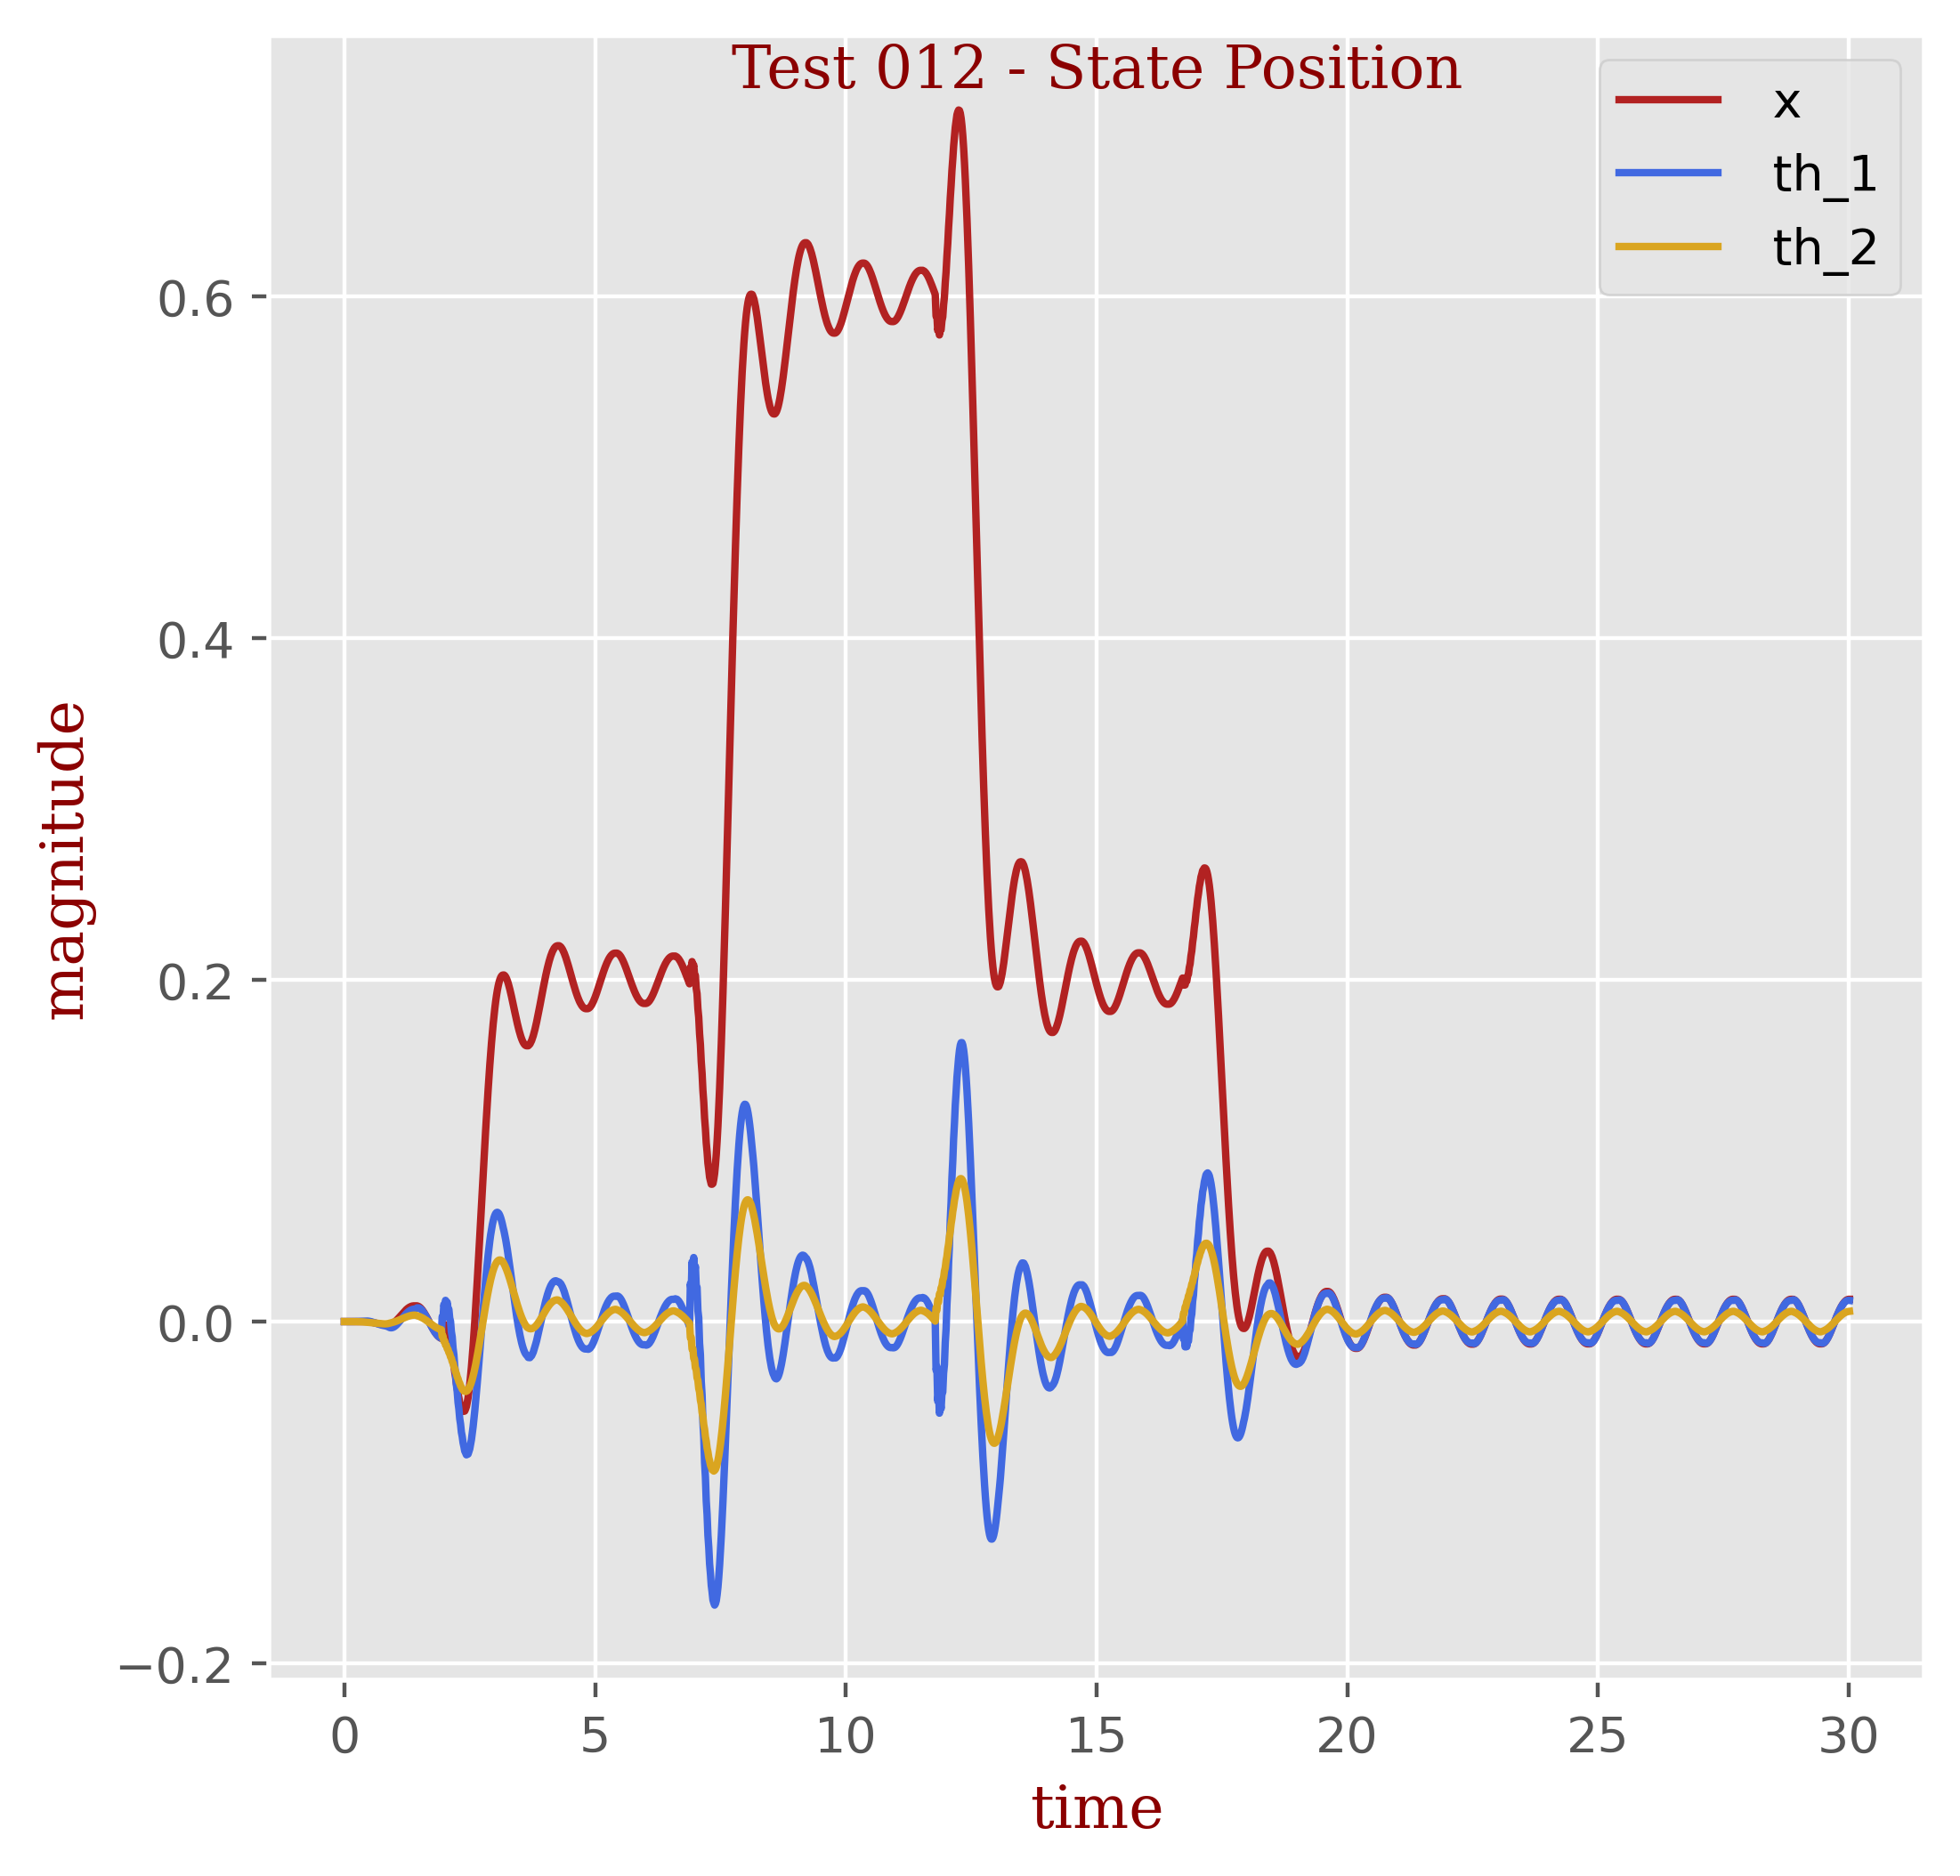
\includegraphics[width=27mm]{Test 012_State_Position.png}}
        \subfigure[\(\dot{q}(t)\)]{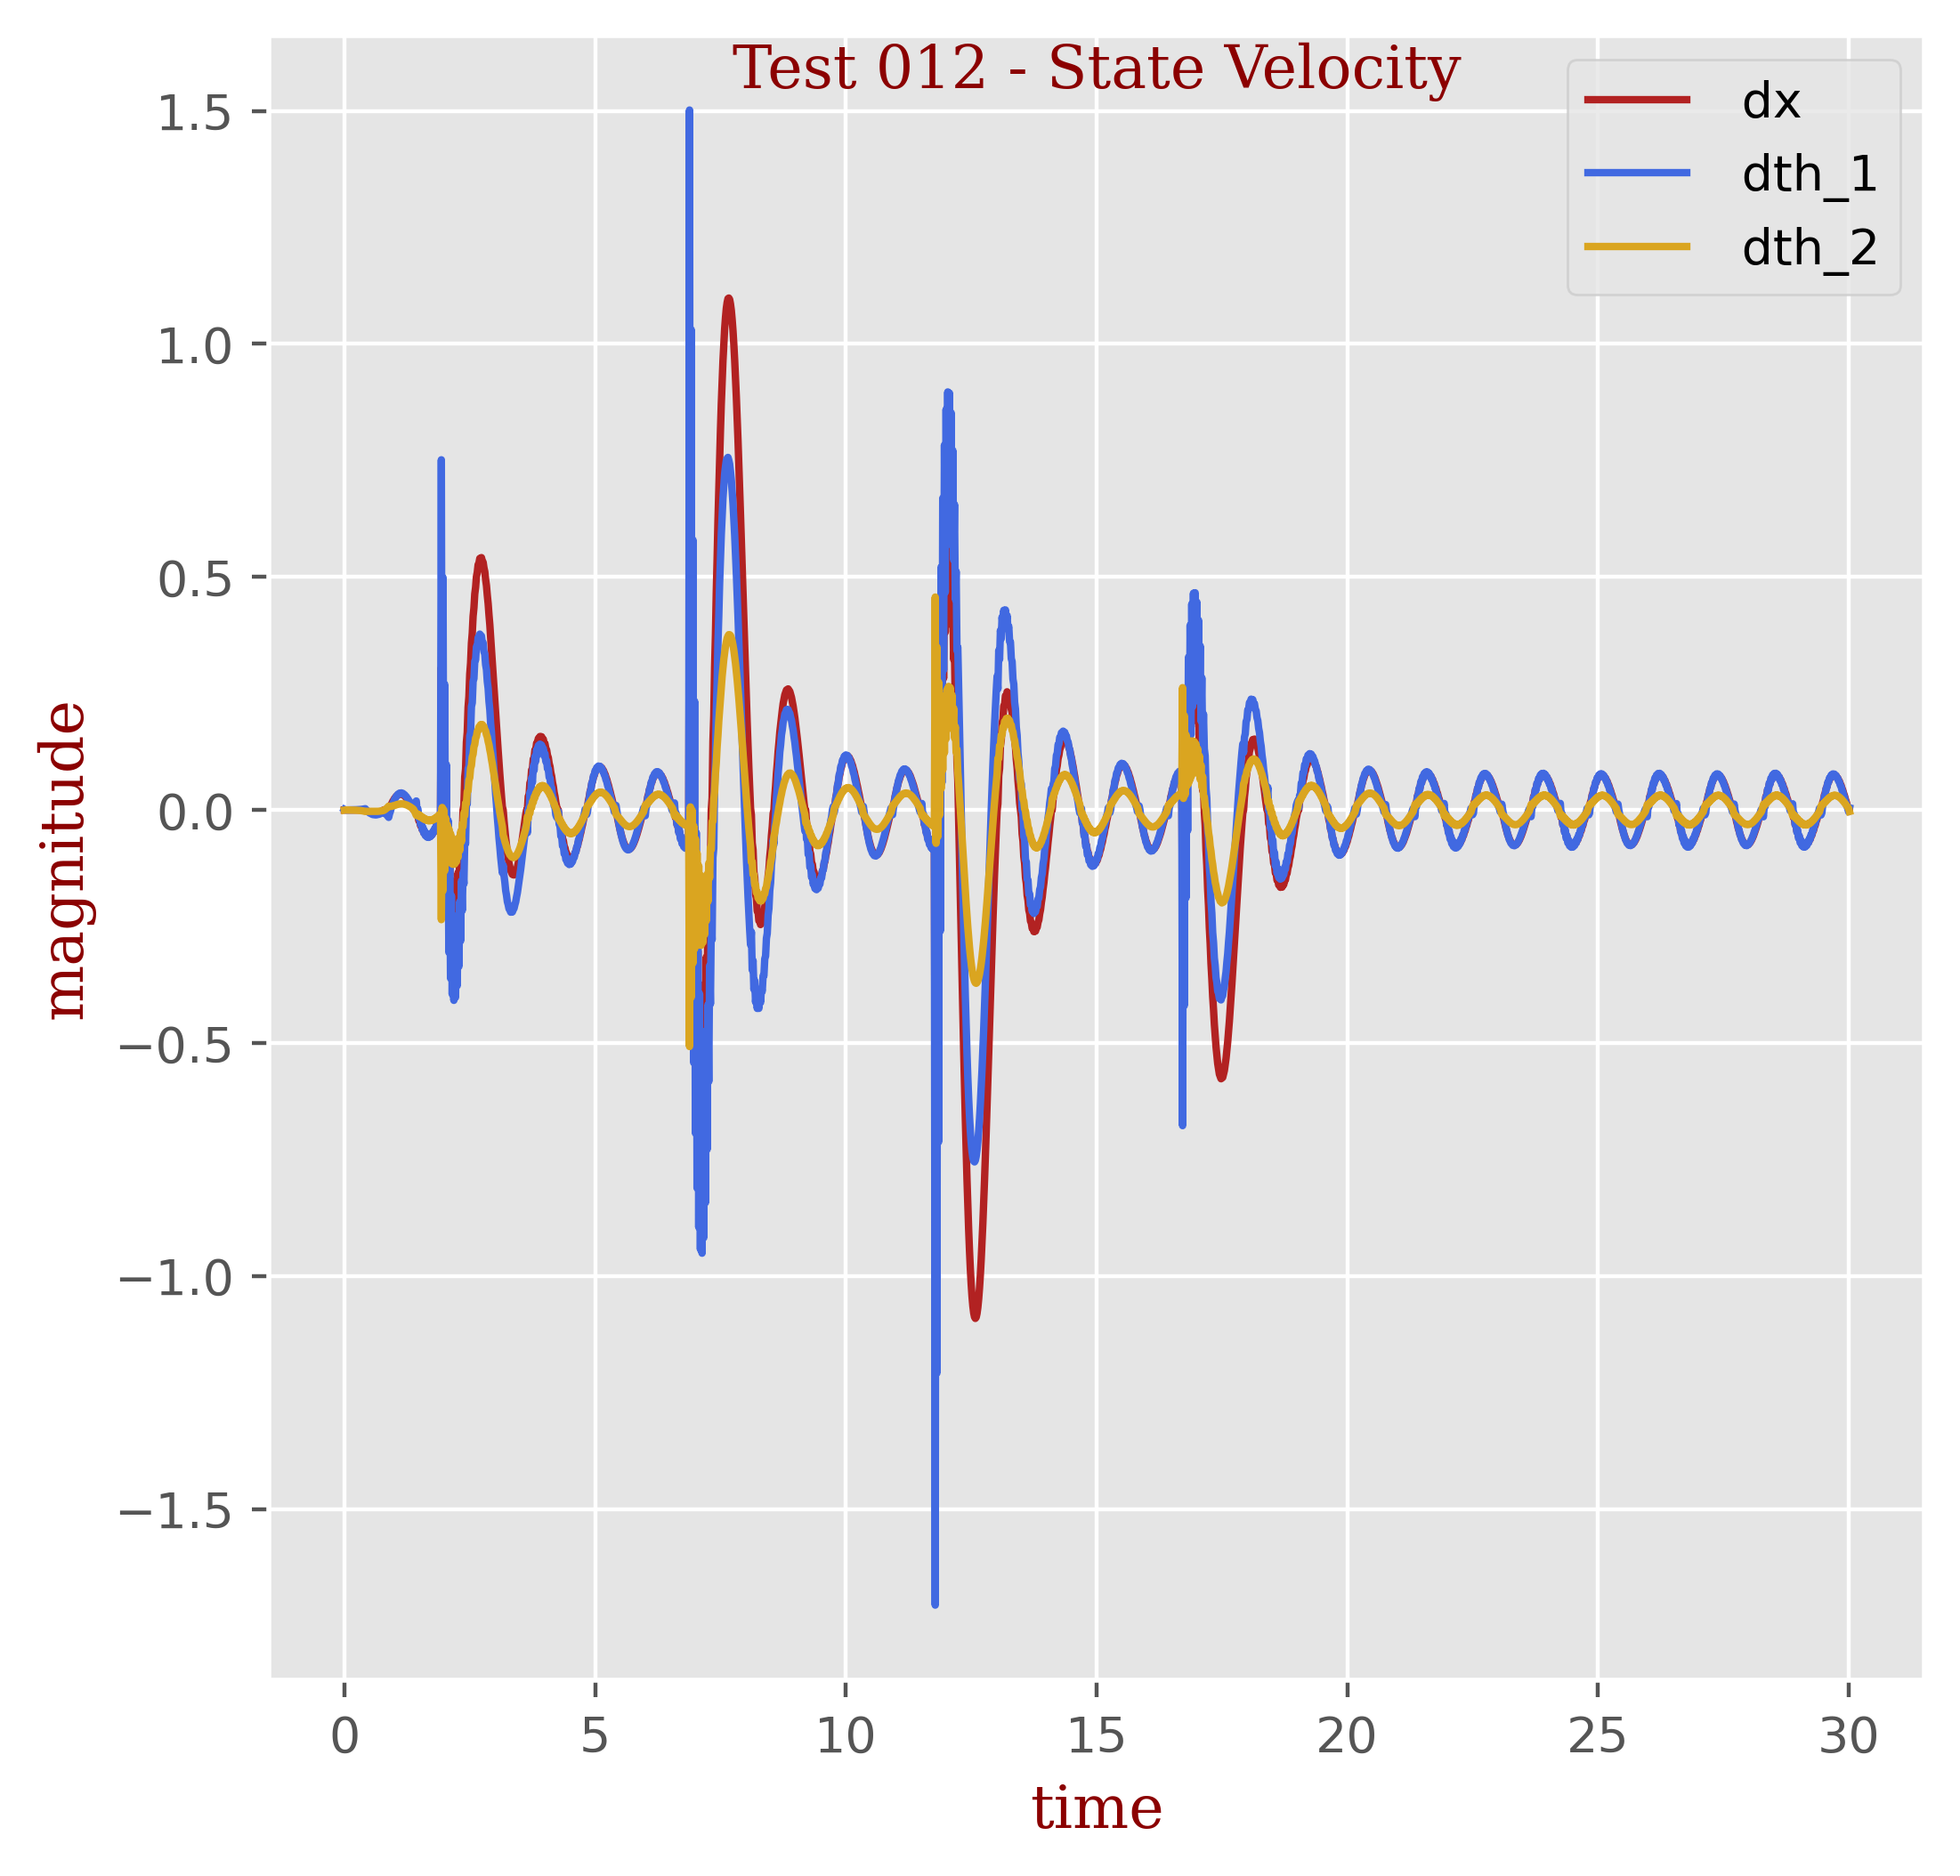
\includegraphics[width=27mm]{Test 012_State_Velocity.png}}
              \subfigure[\(J(t)\)]{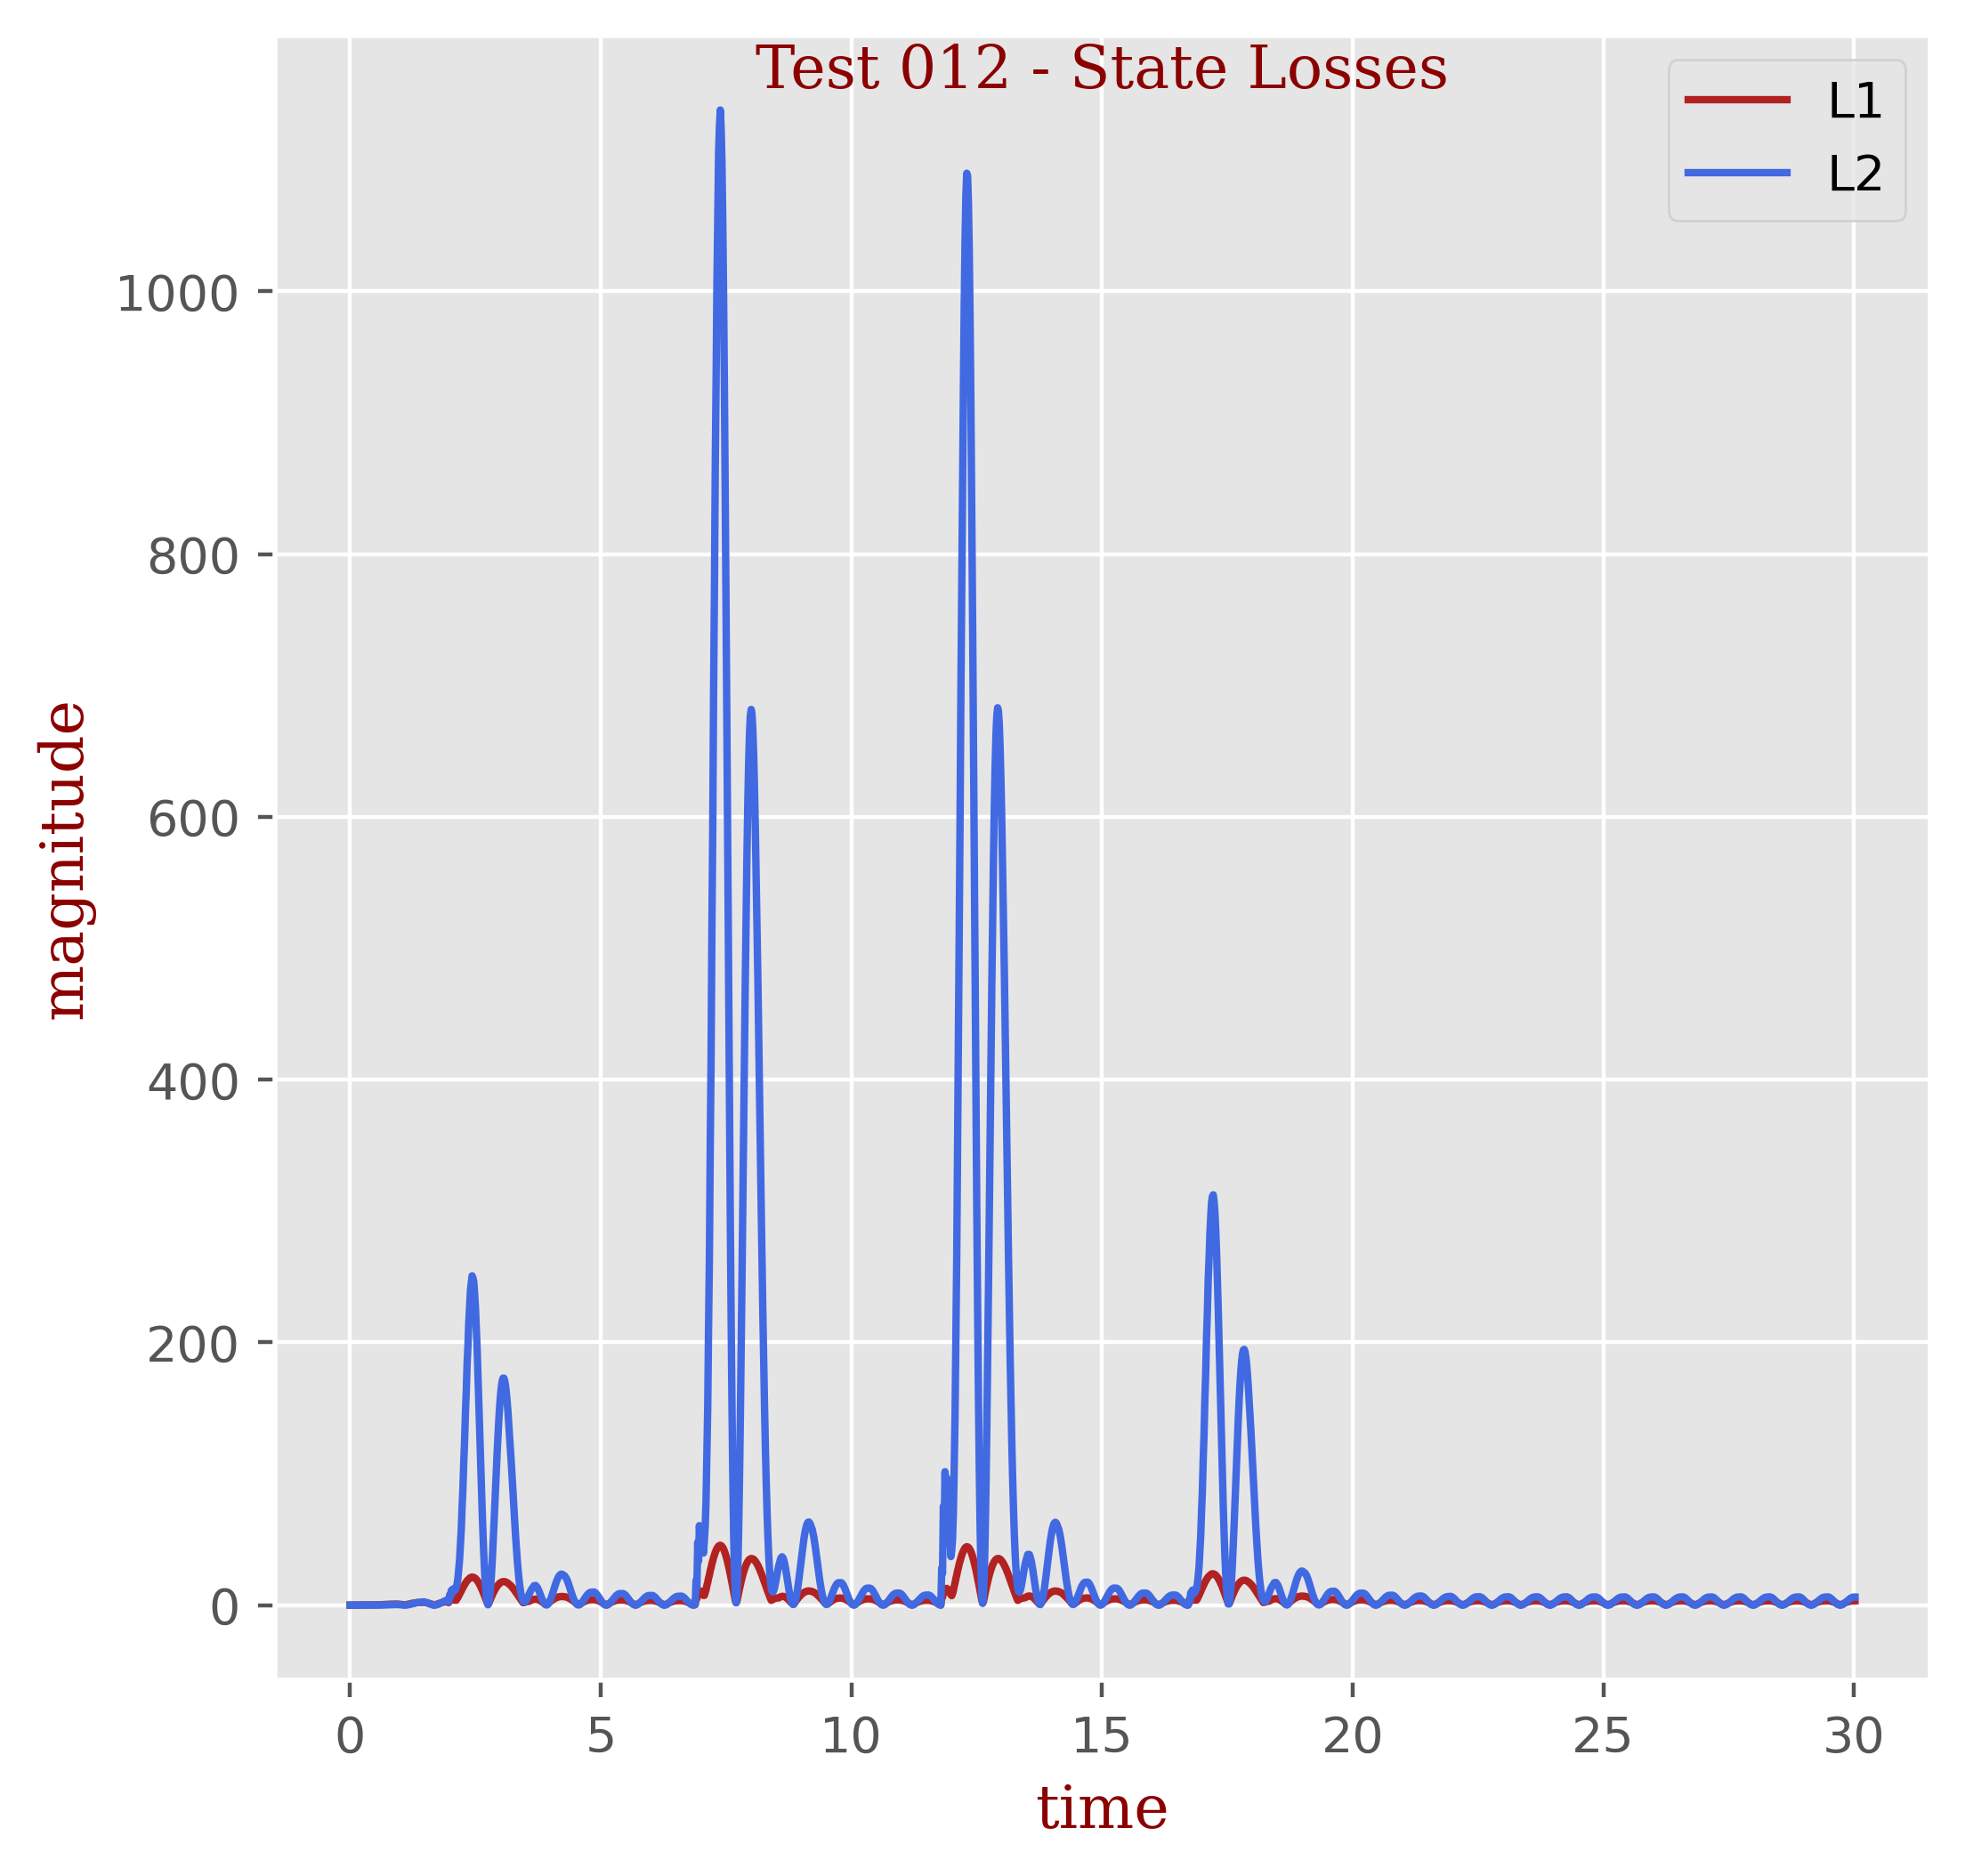
\includegraphics[width=27mm]{Test 012_State_Losses.png}}
                                                       \caption{Test 012}
                                                         \label{fig:t012}
        \end{figure}

\begin{figure}
\centering
      \subfigure[\(q(t)\)]{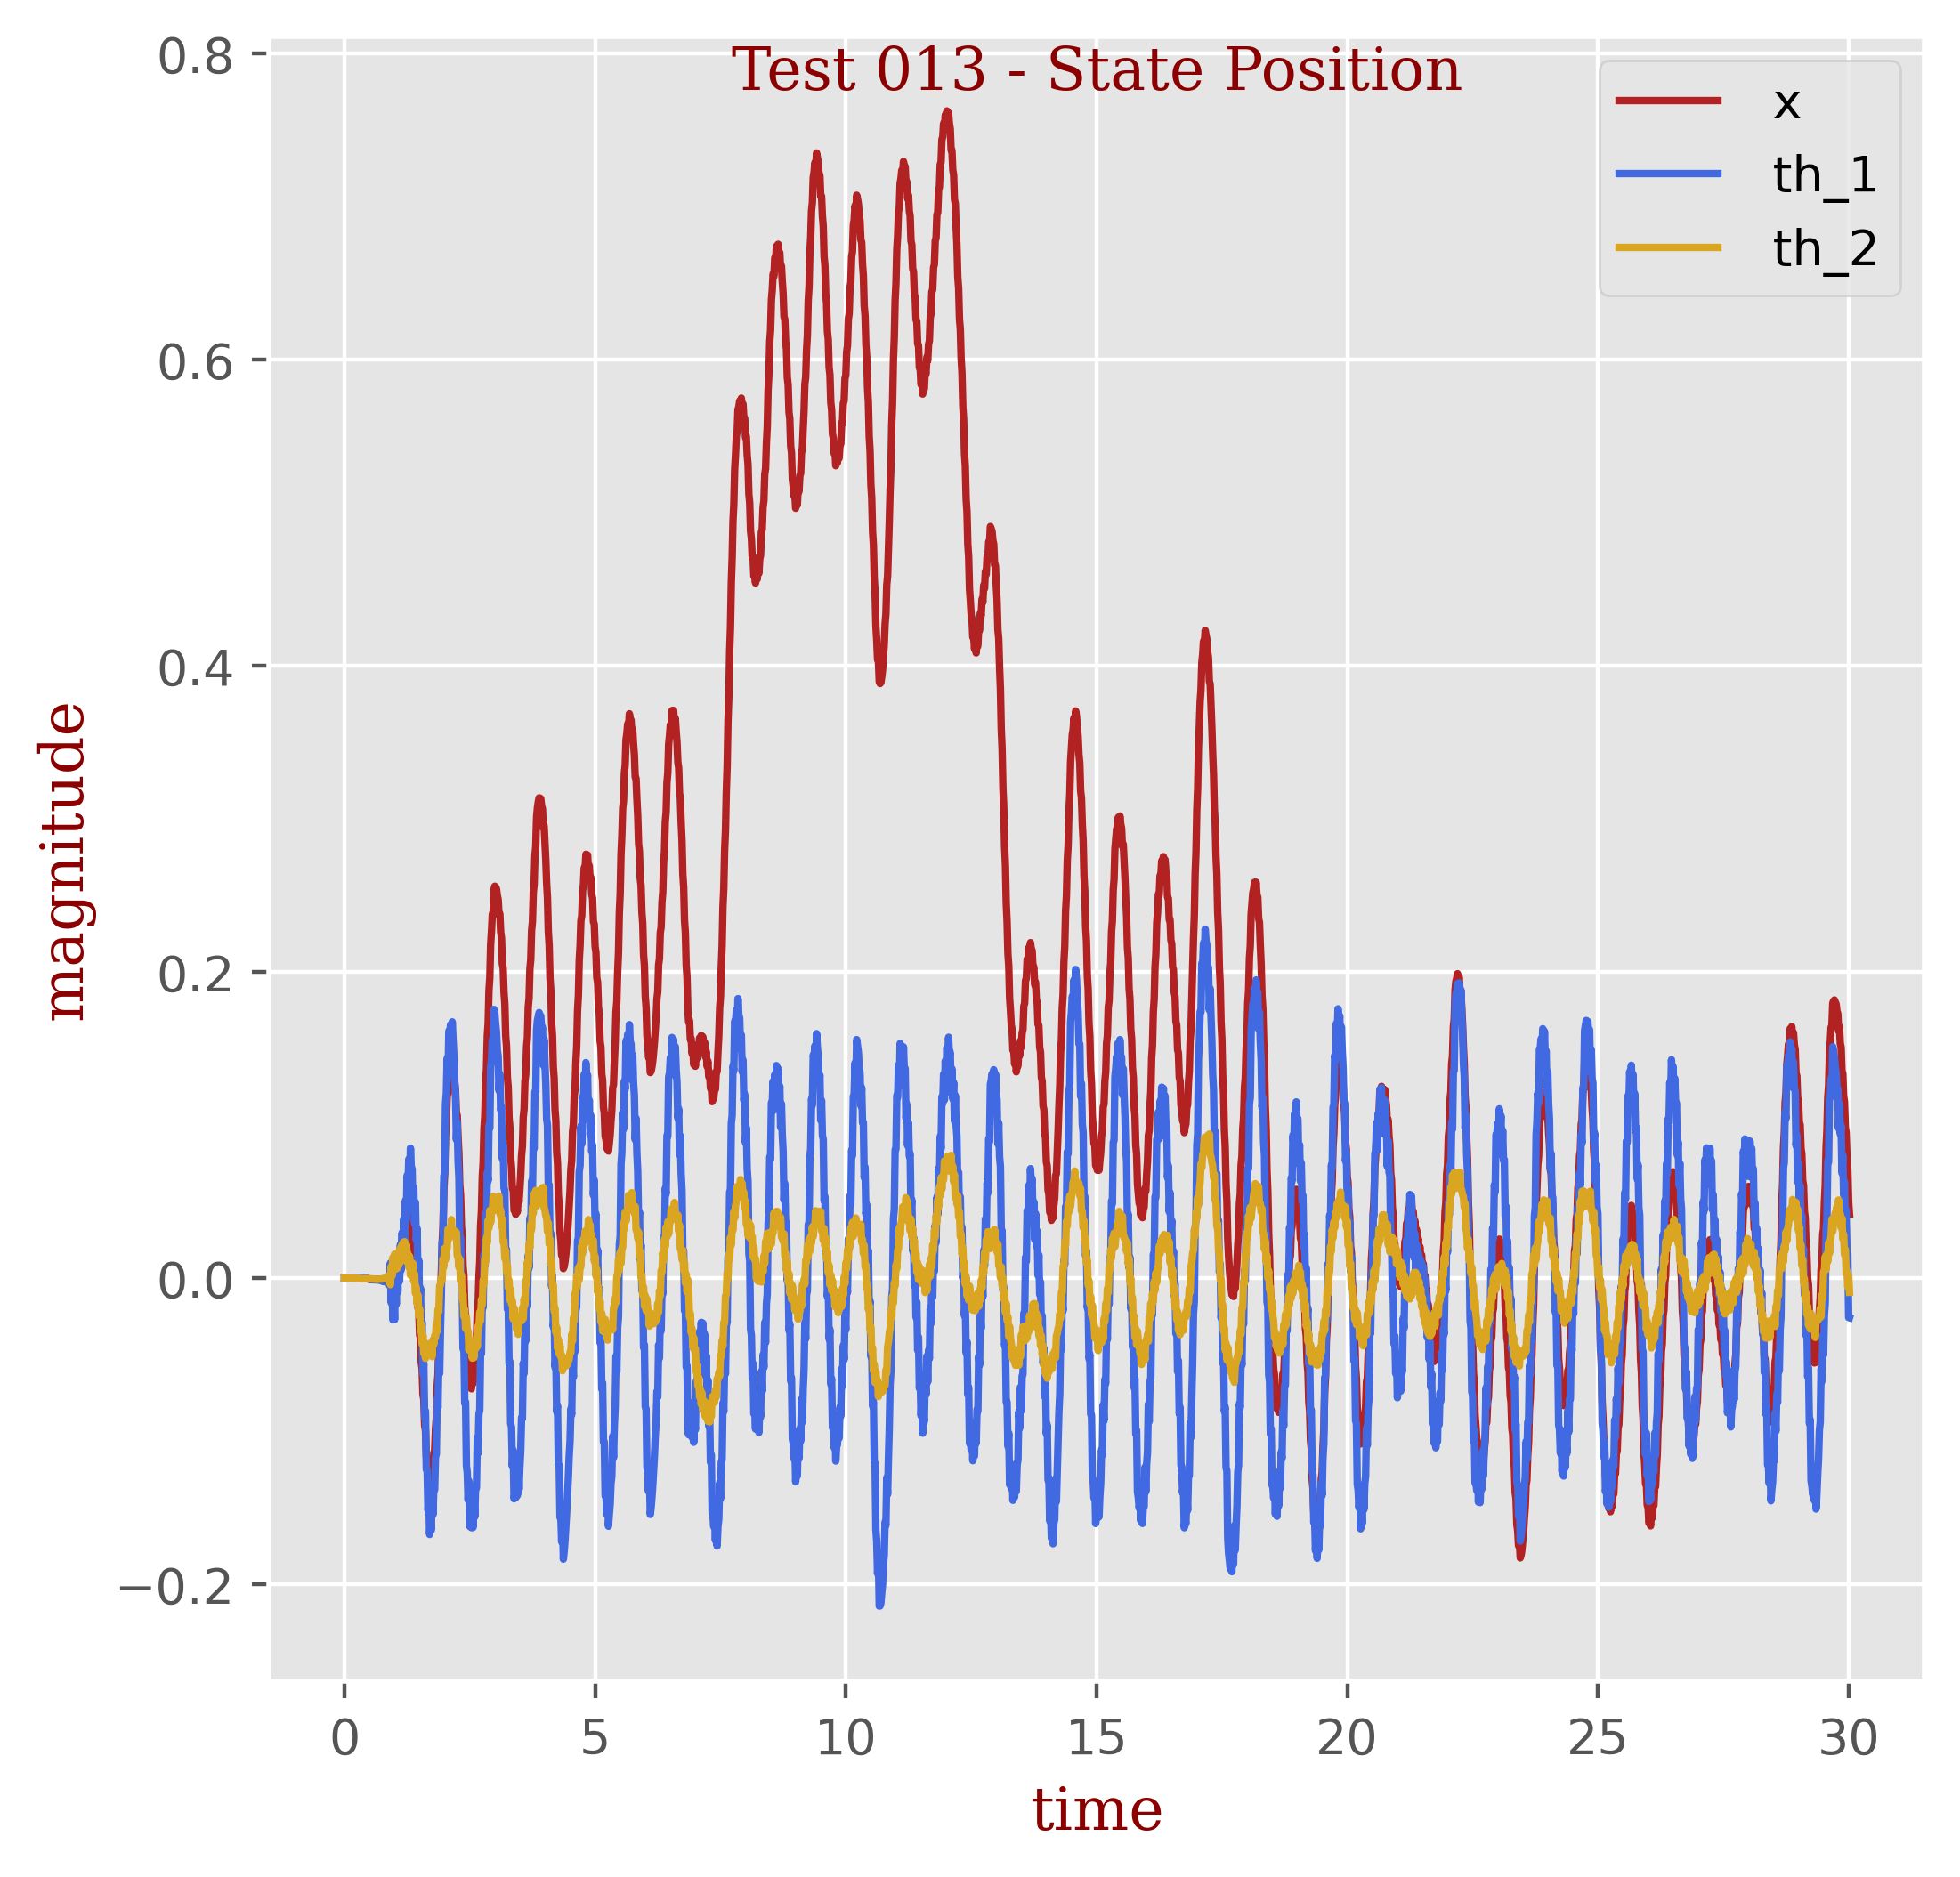
\includegraphics[width=27mm]{Test 013_State_Position.png}}
\subfigure[\(\dot{q}(t)\)]{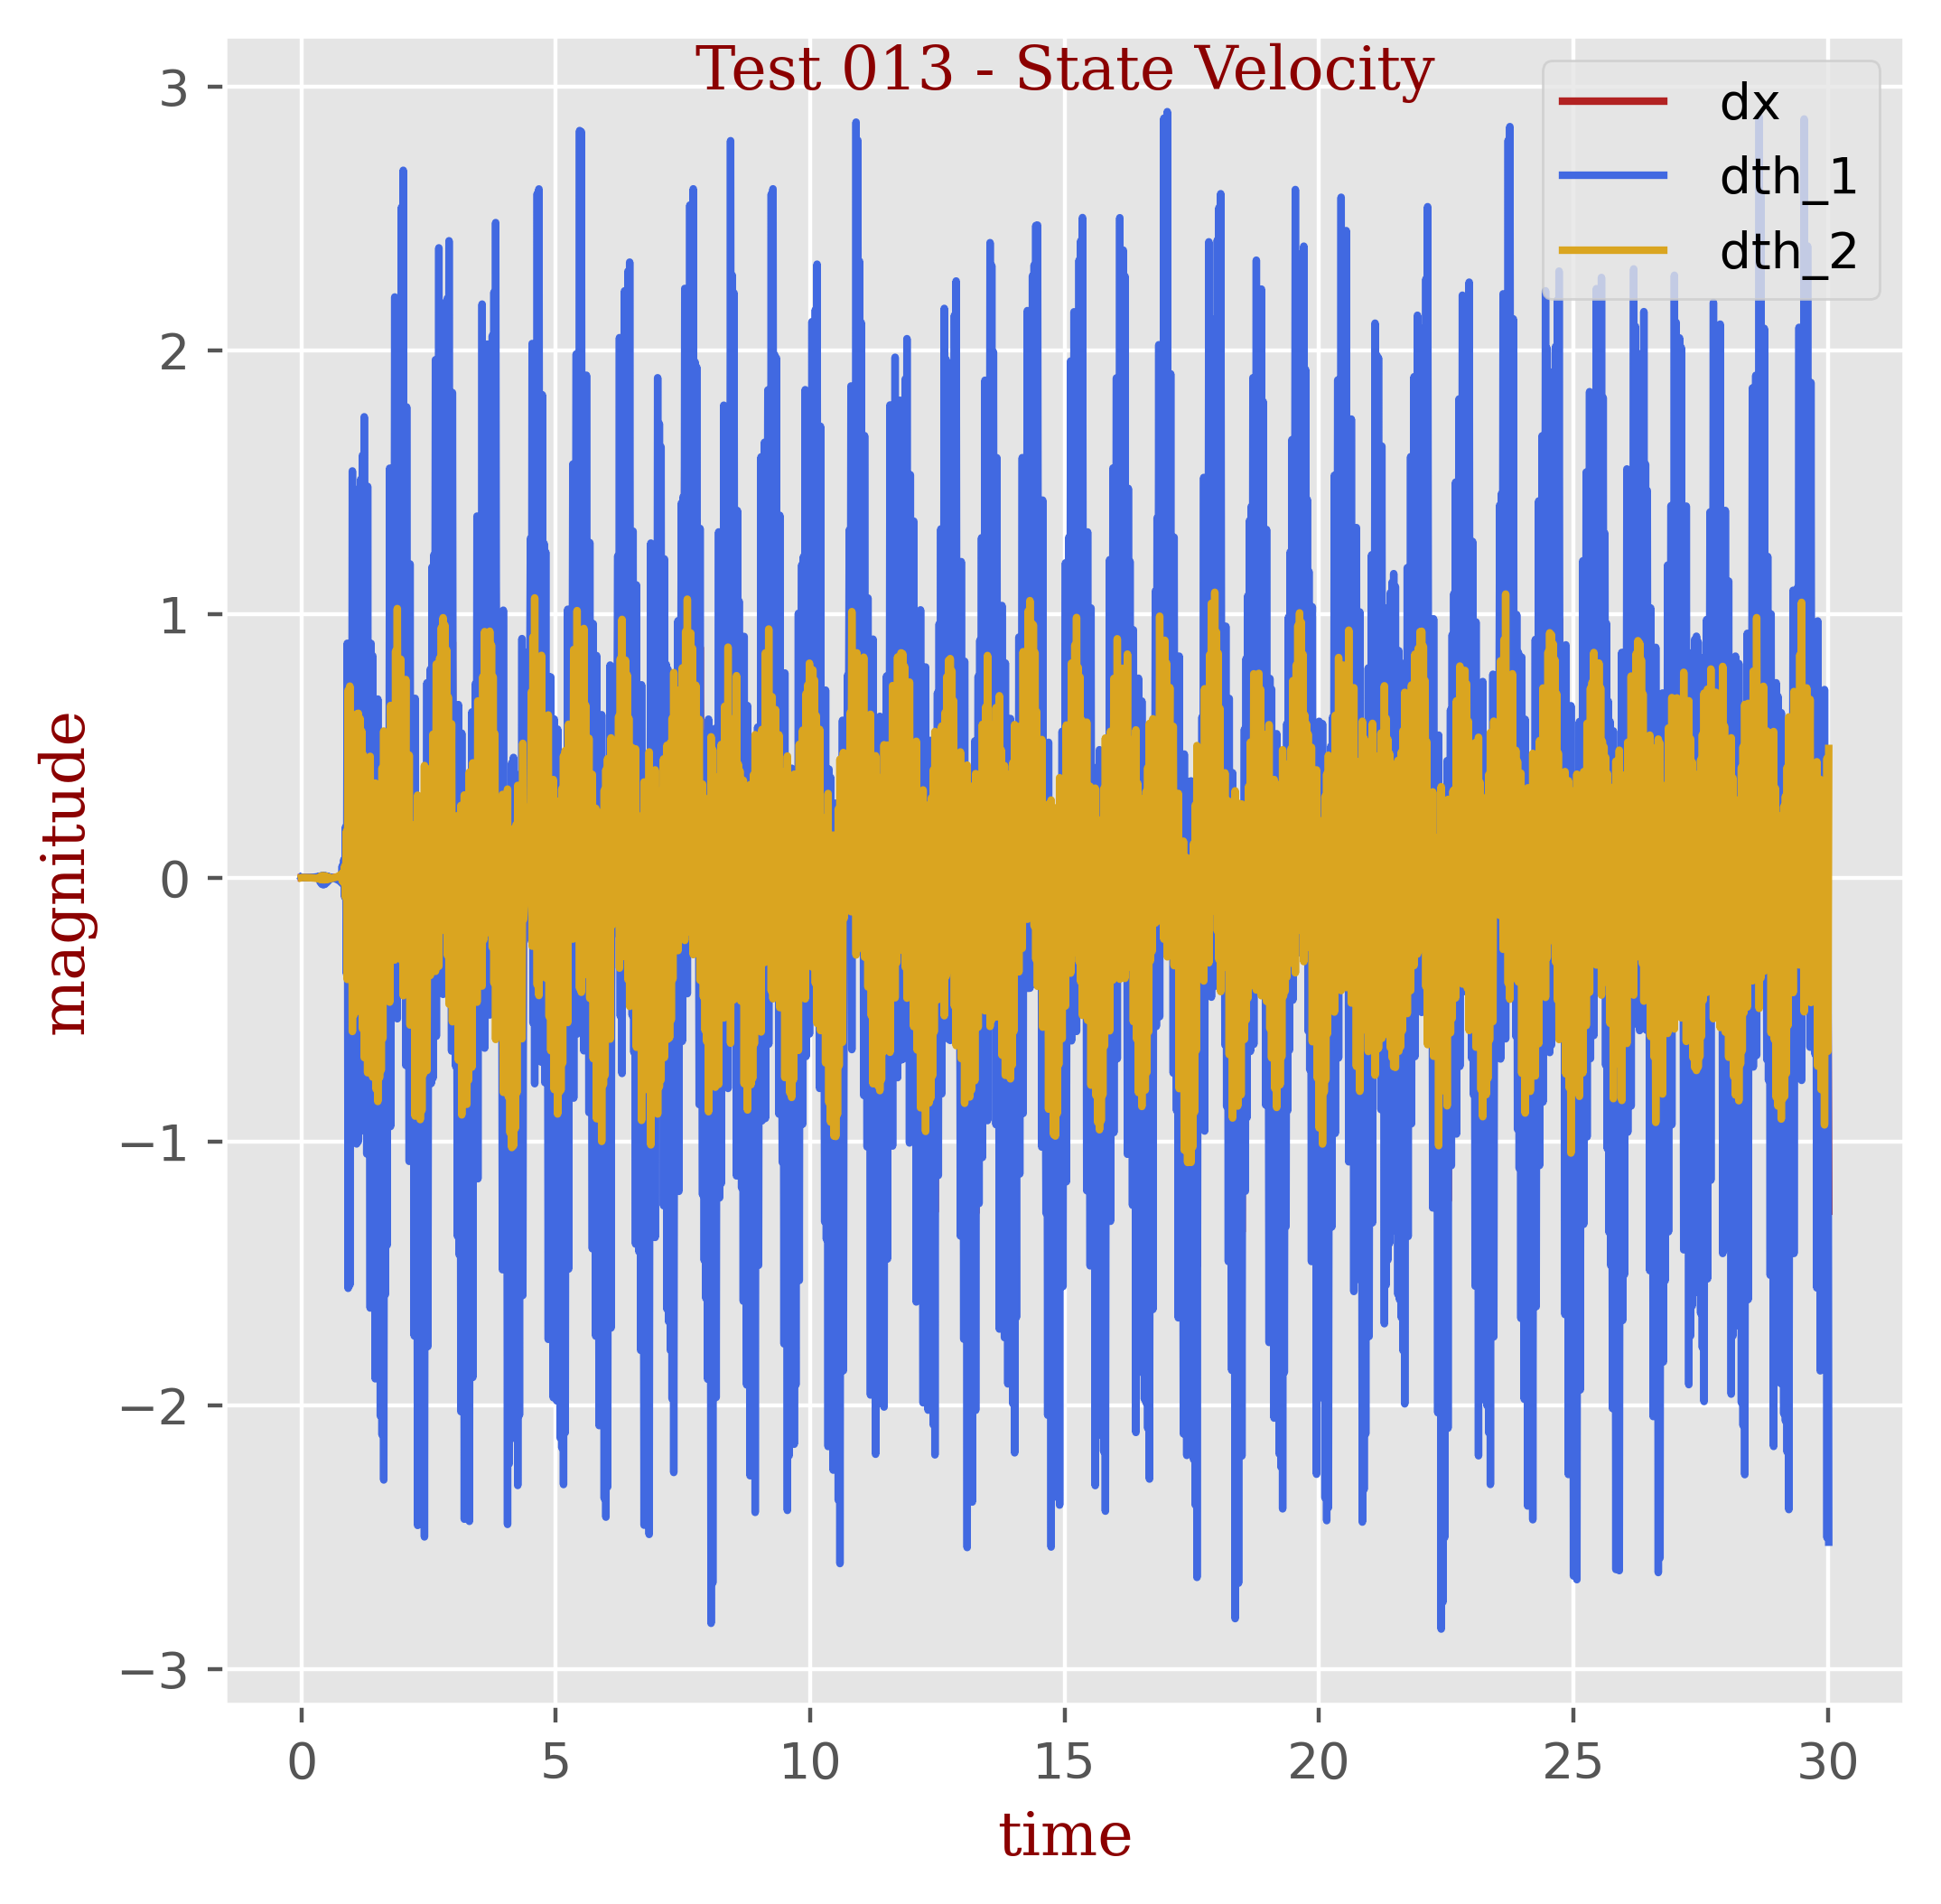
\includegraphics[width=27mm]{Test 013_State_Velocity.png}}
      \subfigure[\(J(t)\)]{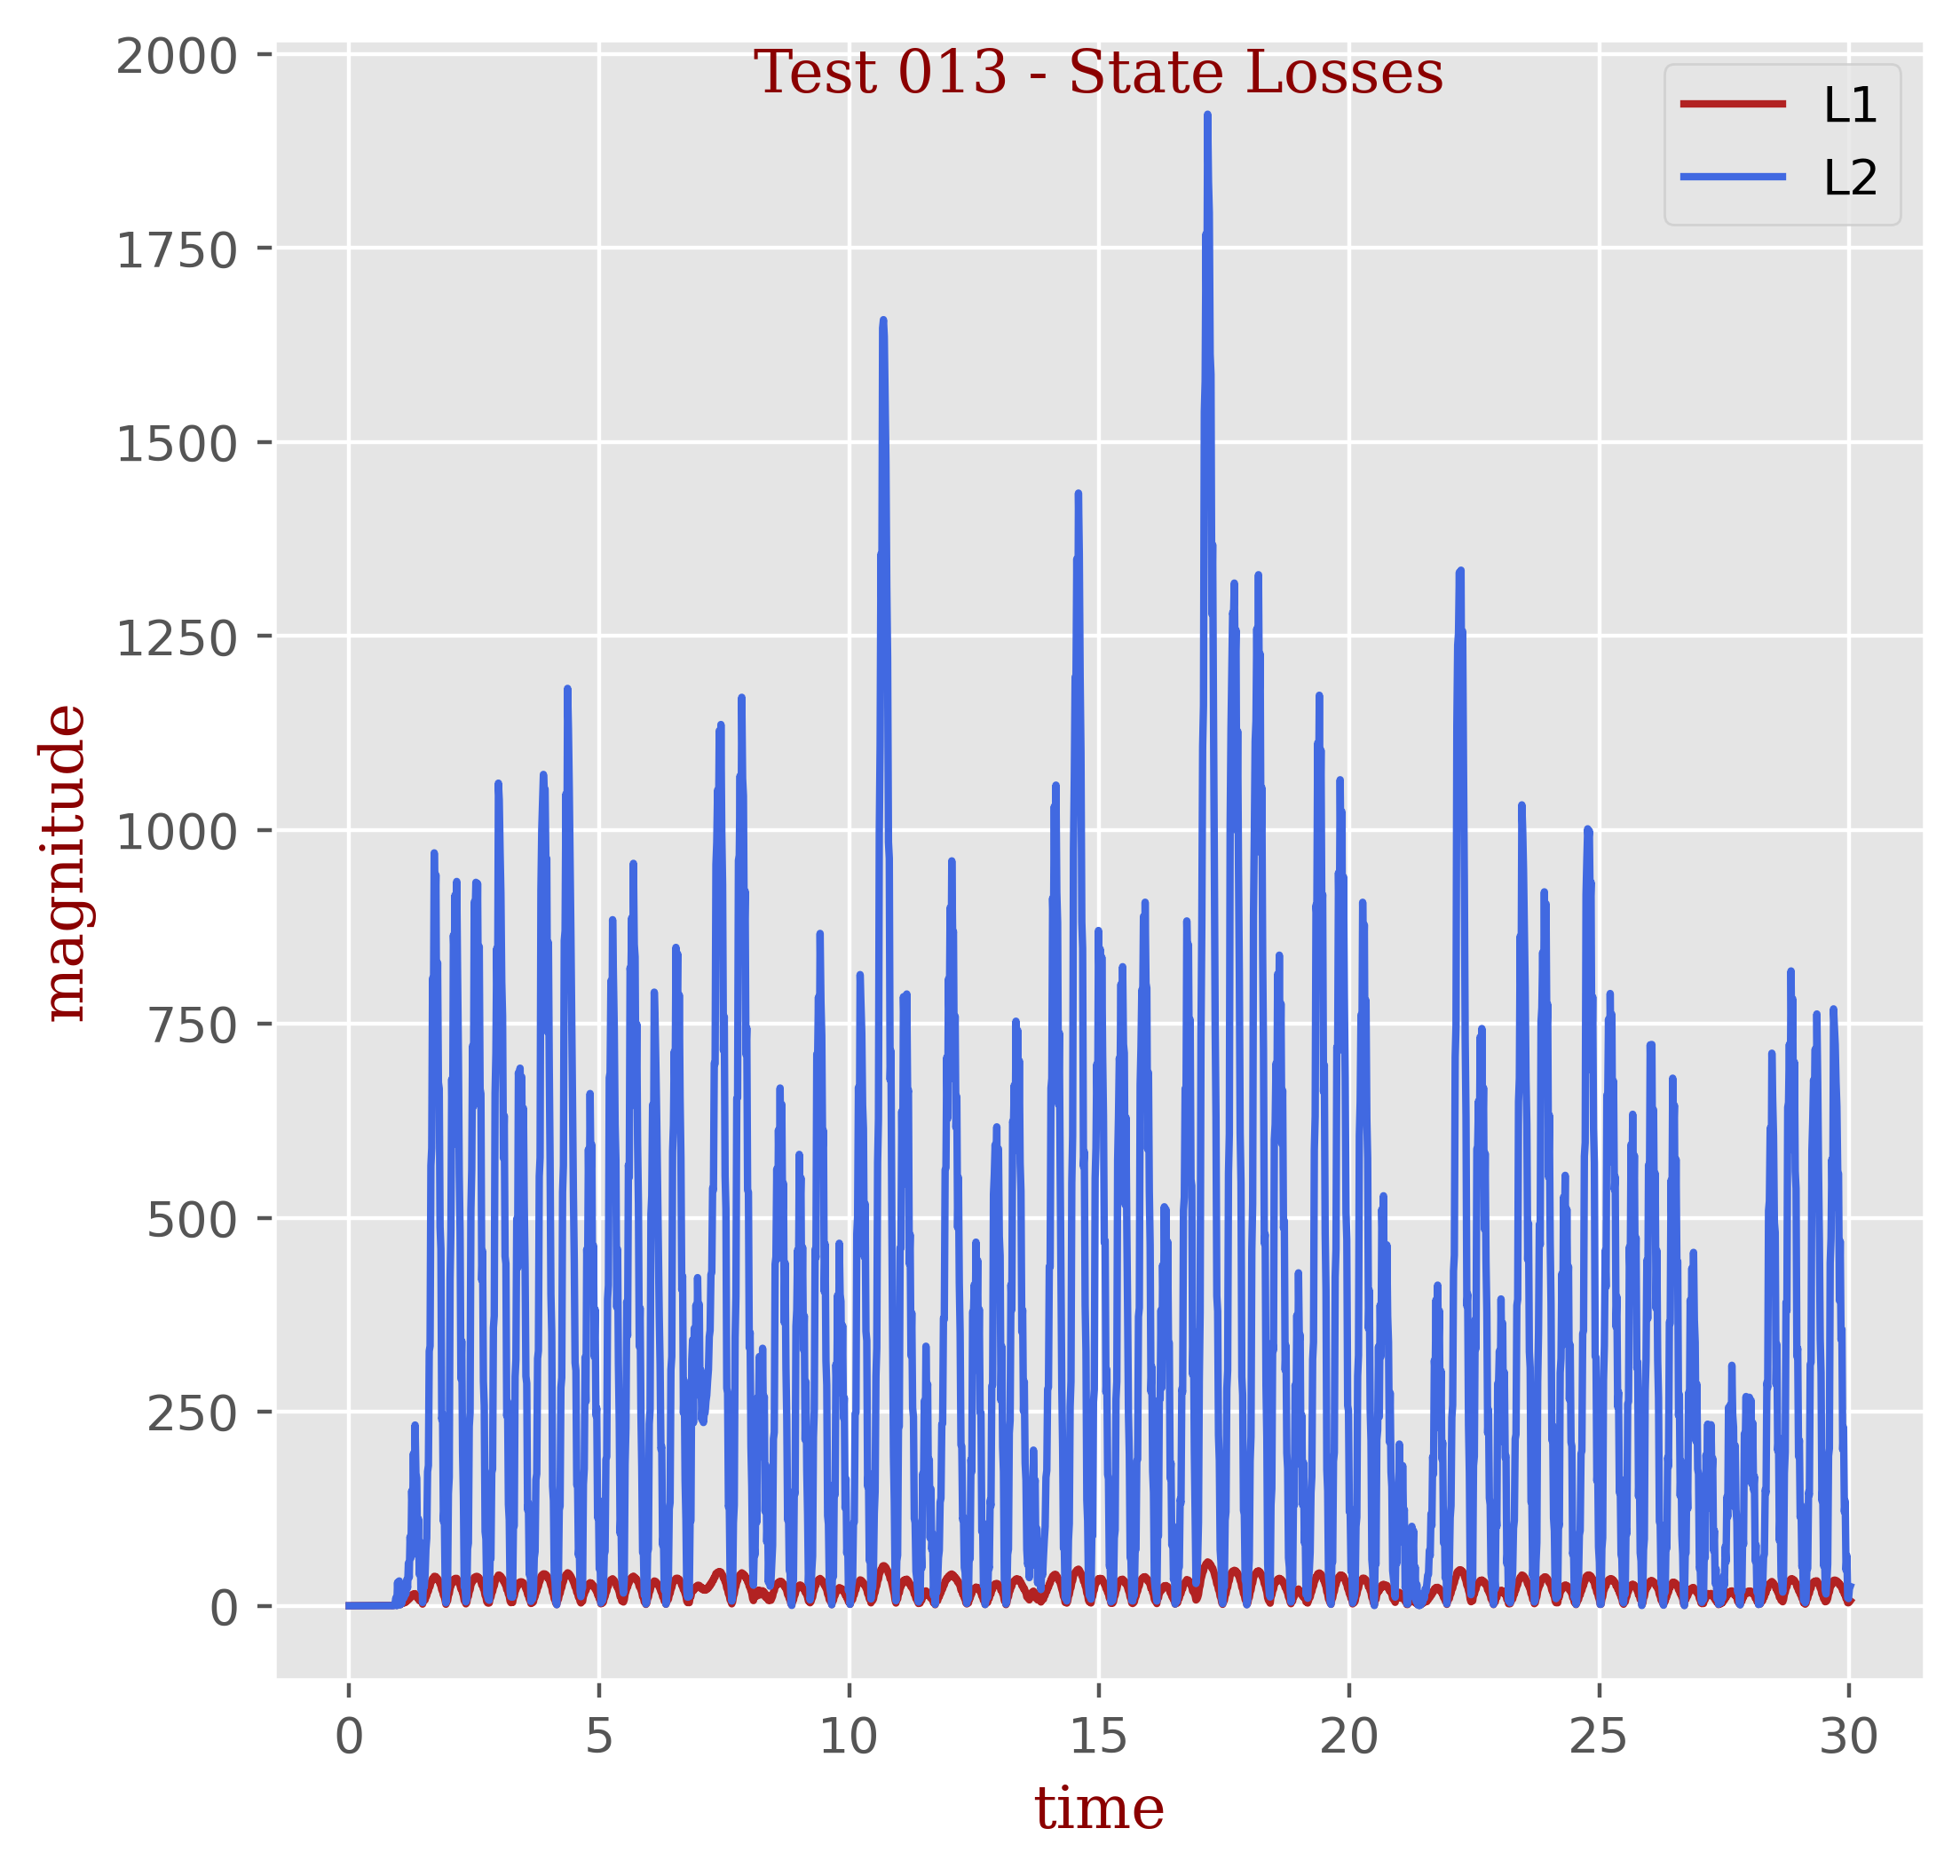
\includegraphics[width=27mm]{Test 013_State_Losses.png}}
                                               \caption{Test 013}
                                                 \label{fig:t013}
\end{figure}


\begin{figure}
    \centering
        \subfigure[\(q(t)\)]{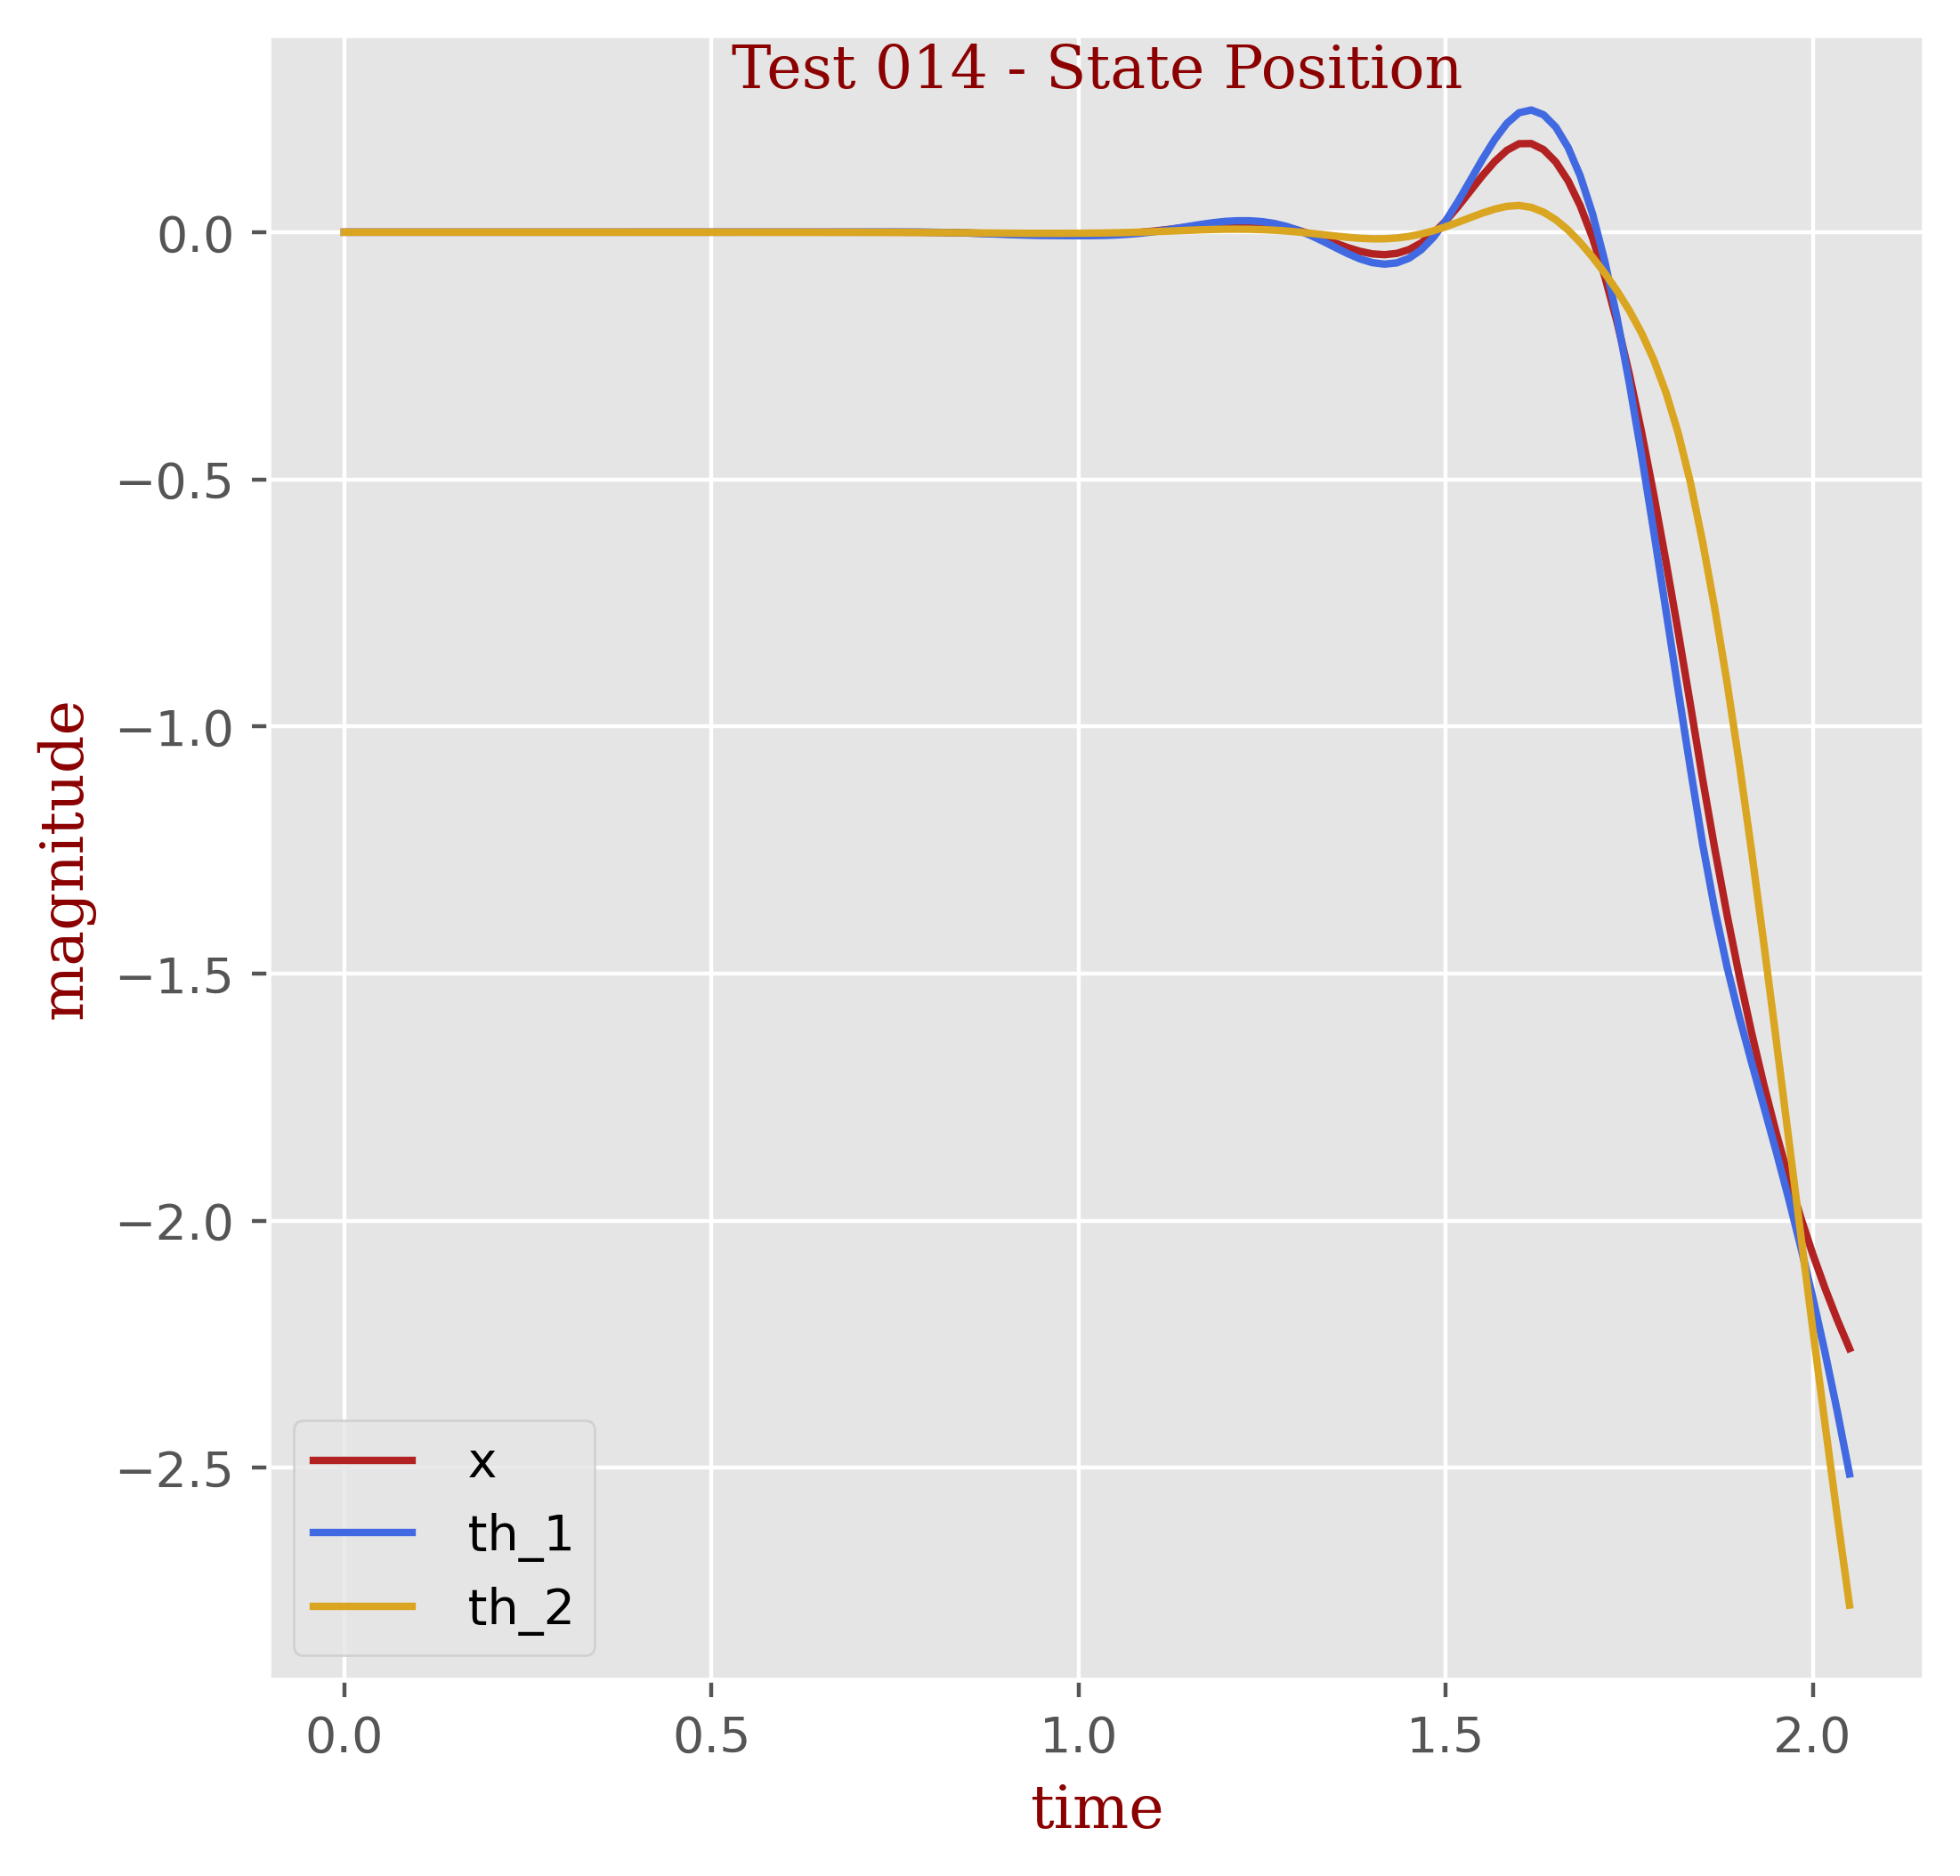
\includegraphics[width=27mm]{Test 014_State_Position.png}}
\subfigure[\(\dot{q}(t)\)]{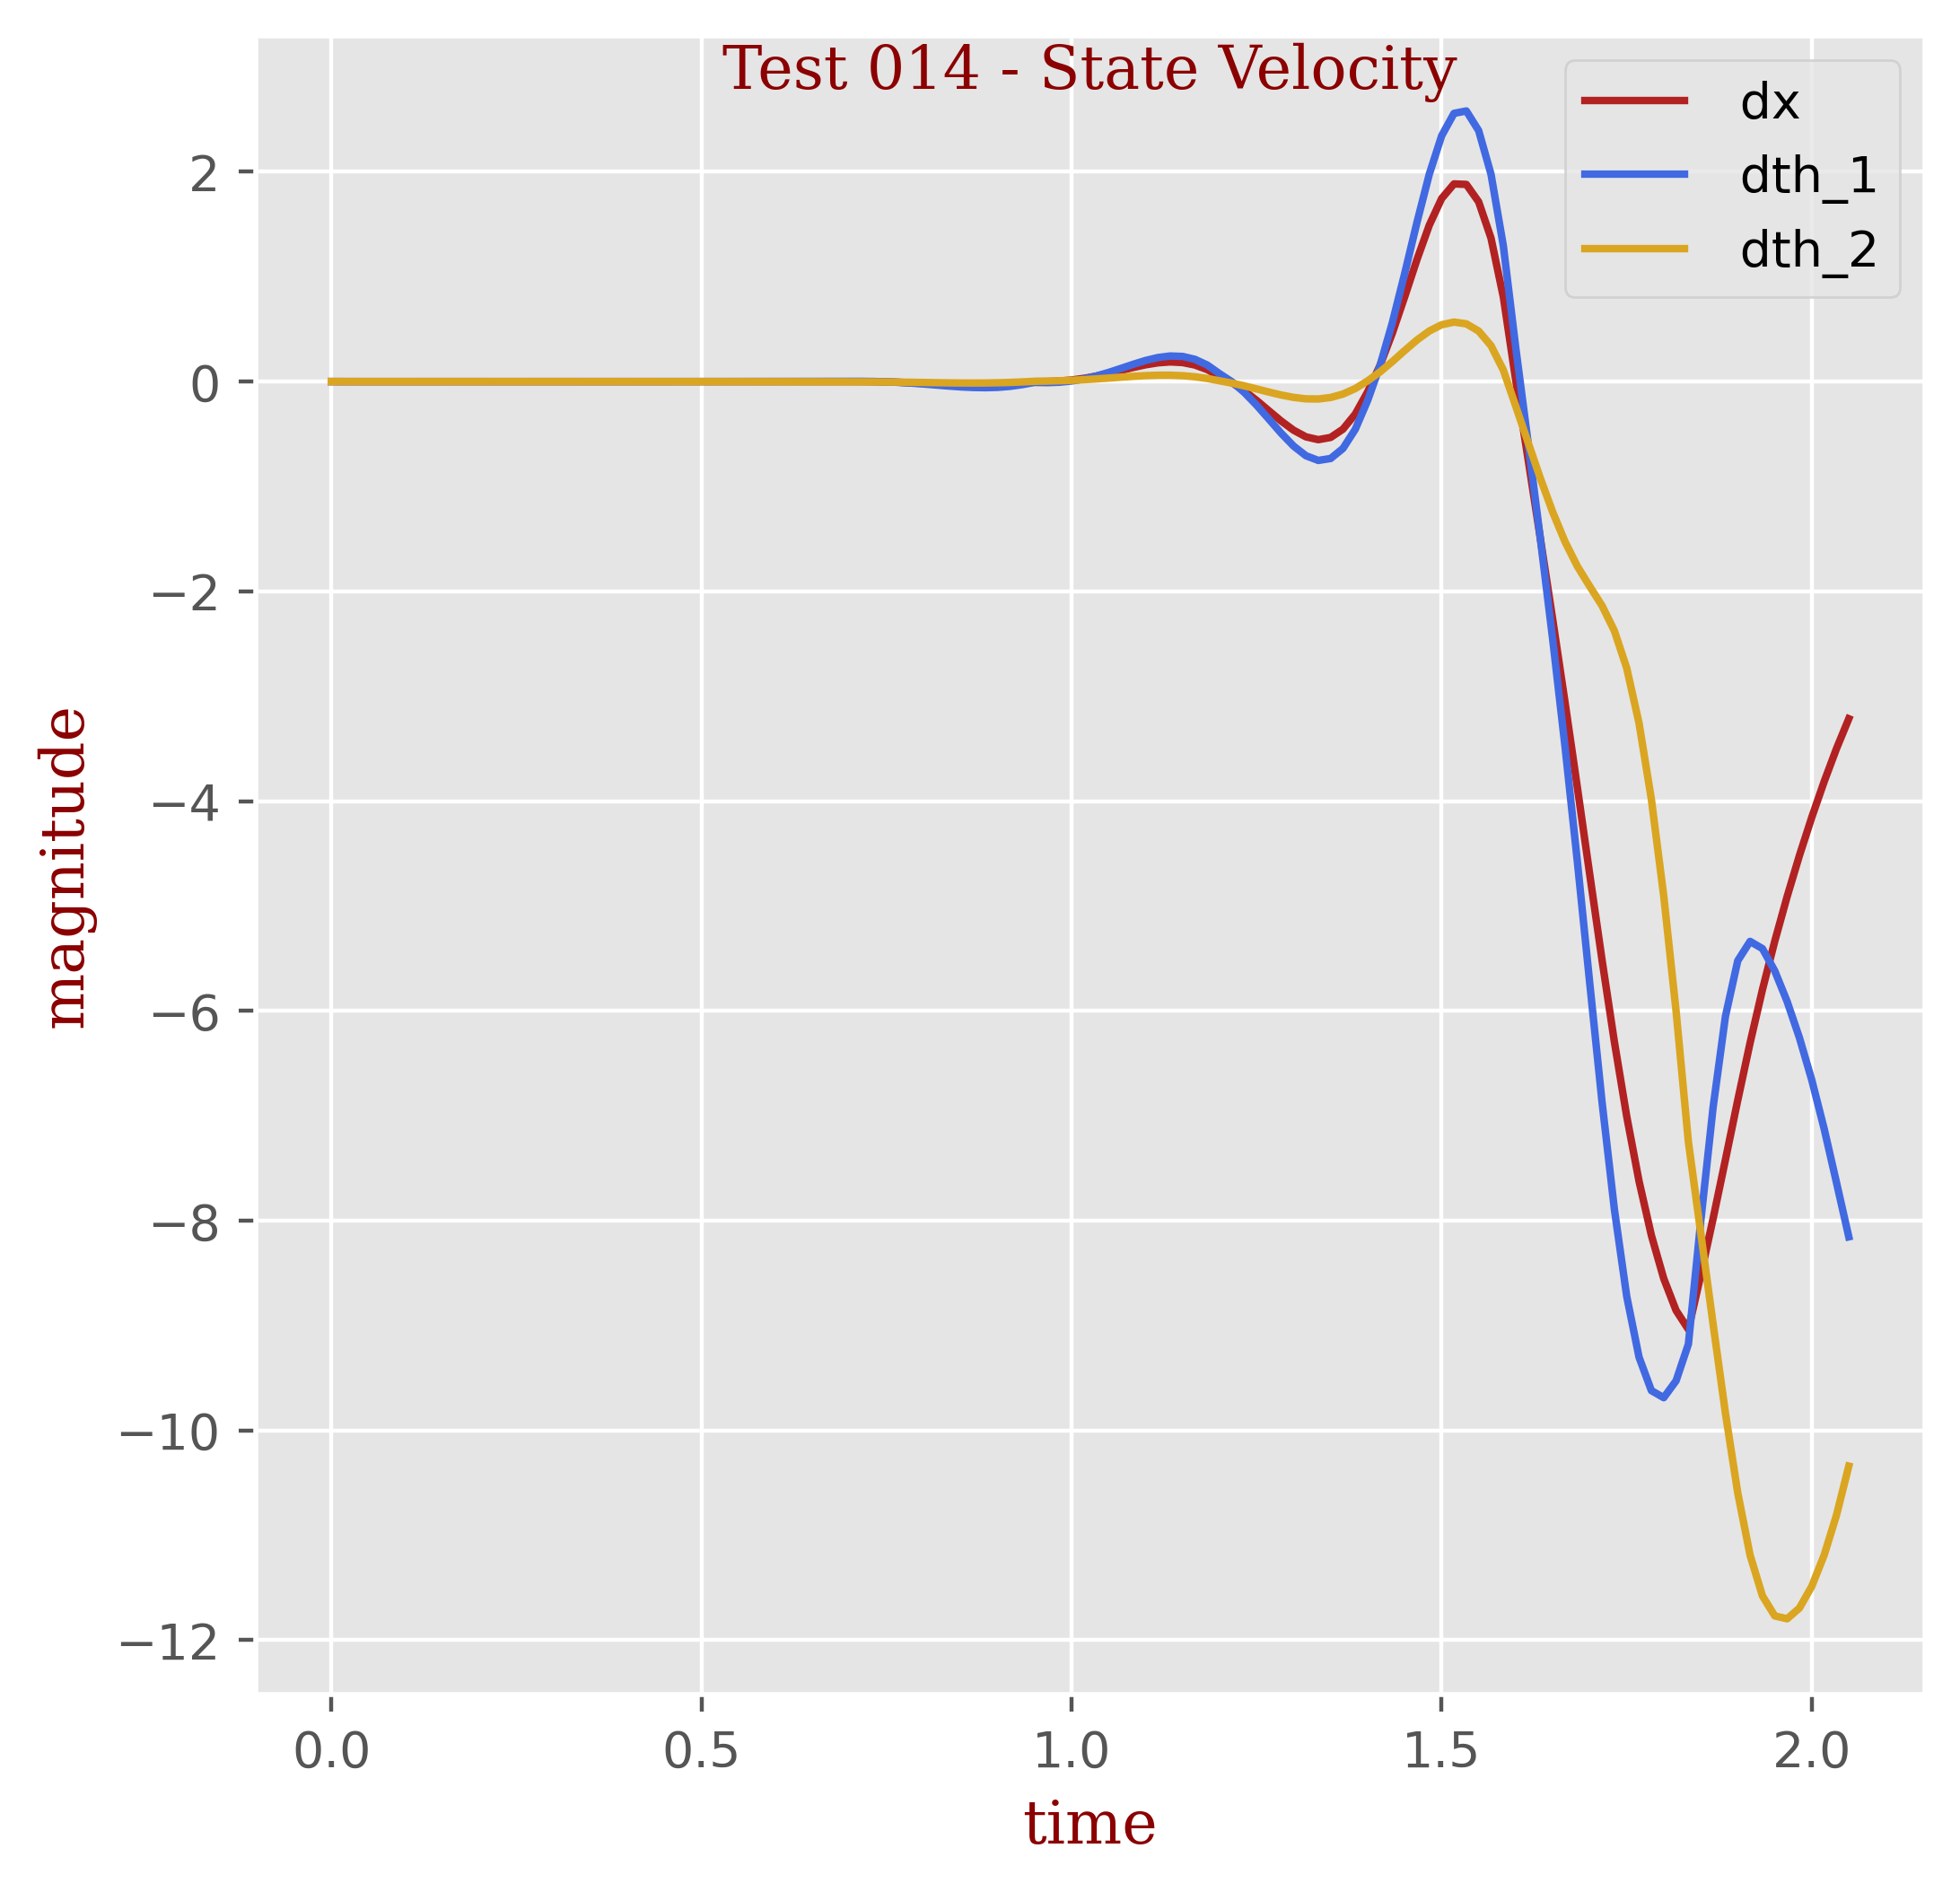
\includegraphics[width=27mm]{Test 014_State_Velocity.png}}
        \subfigure[\(J(t)\)]{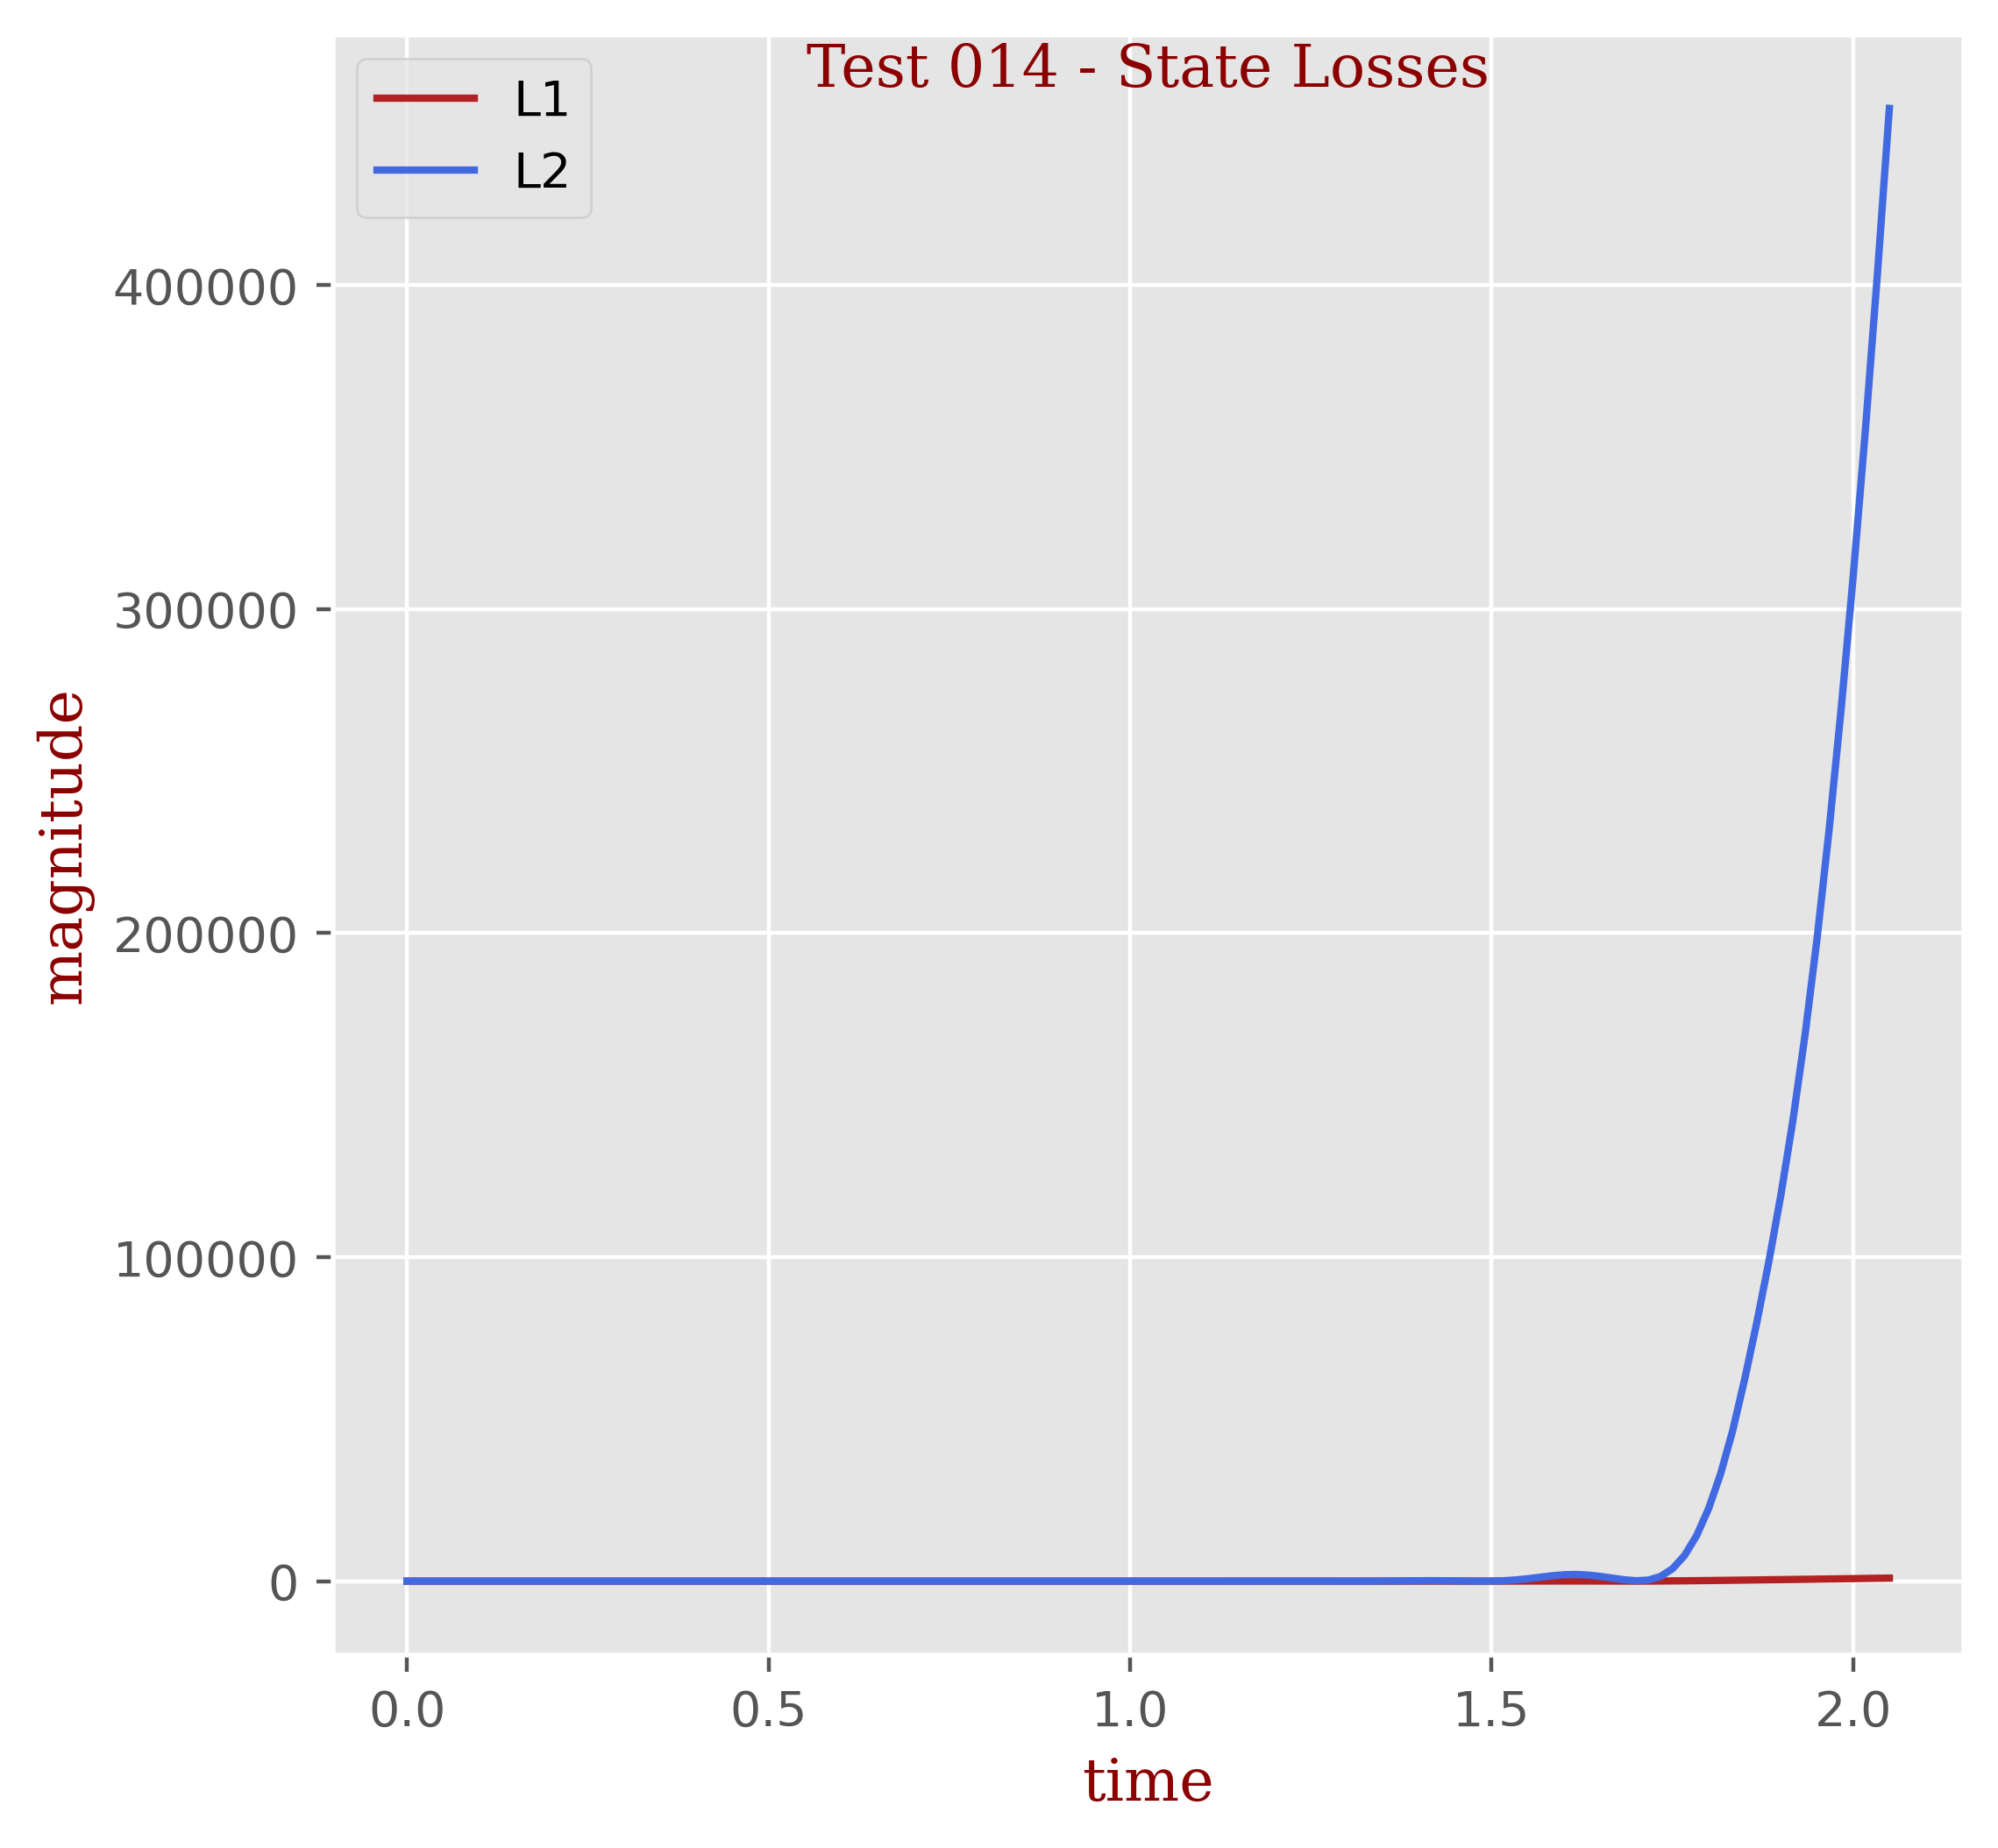
\includegraphics[width=27mm]{Test 014_State_Losses.png}}
                                                \caption{Test 014}
                                                    \label{fig:t014}
    \end{figure}
